%%%%%%%%%%%%%%%%%%%%%%%%%%%%%%%%%%%%%%%%%
% This is the LaTeX template of Jonas Schultheiss. It'll be used for the IPA and VA.
% 
% This template can be downloaded here:
% https://github.com/
% 
% This template is heavily inspired by Marco Roth's template:
% https://github.com/marcoroth
%
% Template license:
% MIT
% https://github.com/jonasschultheiss/LaTeX-Template/blob/master/LICENSE
% ./LICENSE
%%%%%%%%%%%%%%%%%%%%%%%%%%%%%%%%%%%%%%%%%

%%%%%%%%%%%%%%%%%%%%%%
% Document & Variables
%%%%%%%%%%%%%%%%%%%%%%

\newcommand{\version}{0.4.4}
\newcommand{\docdate}{\today}
\newcommand{\docname}{SkyPulse Technologies}
\newcommand{\compiledfilename}{wr-skypulse-technologies.pdf}
\newcommand{\task}{SkyPulse Technologies} % e.g. Modul 152/IPA/...
\newcommand{\taskname}{Creating a startup business plan}
\newcommand{\clientlogopath}{./images/bbzbl.png}
\newcommand{\all}{F. Boni, X. Gautschy, C. Moser, J.Schultheiss}
\newcommand{\fabian}{Fabian Boni}
\newcommand{\xenia}{Xenia Gautschy}
\newcommand{\celine}{Céline Moser}
\newcommand{\jonas}{Jonas Schultheiss}
\newcommand{\expert}{Olga Samuel}
\newcommand{\docauthor}{\all}


%%%%%%%%%%
% Packages
%%%%%%%%%%

\usepackage[
  a4paper,
  left=20mm,
  right=20mm,
  top=35mm,
  bottom=35mm,
  headheight=35mm
]{geometry}
\usepackage[utf8]{inputenc}
\usepackage[babel,english]{csquotes}
\usepackage[english]{babel}
\usepackage[printonlyused]{acronym}
\usepackage[section]{placeins}
\usepackage[Conny]{fncychap}
\usepackage[T1]{fontenc}
\usepackage[T1]{fontenc}
\usepackage[table]{xcolor}
\usepackage{caption}
\usepackage{color}
\usepackage{fancyhdr}
\usepackage{graphics}
\usepackage{graphicx}
\usepackage{helvet}
\usepackage{lastpage}
\usepackage{lipsum}
\usepackage{listings}
\usepackage{multicol}
\usepackage{multirow}
\usepackage{parskip}
\usepackage{pdfpages}
\usepackage{pifont}
\usepackage{tabularx}
\usepackage{longtable}
\usepackage{tocloft}
\usepackage{xurl}
\usepackage{wrapfig}
\usepackage{xcolor}
\usepackage{afterpage}
\usepackage[backend=biber, style=numeric]{biblatex}
\usepackage{suffix}
\usepackage{ragged2e}
\usepackage{float}
\usepackage[
  left = \flqq{},% 
  right = \frqq{},% 
  leftsub = \flq{},% 
  rightsub = \frq{} %
]{dirtytalk}

%%%%%%%%
% Colors
%%%%%%%%

\definecolor{lightgray}{RGB}{224,224,224}
\definecolor{darkgray}{RGB}{192,192,192}

\renewcommand{\listfigurename}{List of figures}


%%%%%%%%%%%%%%%%%%%
% Headers & Footers
%%%%%%%%%%%%%%%%%%%

\pagestyle{fancy}
\renewcommand{\chapterpagestyle}{fancy}
\renewcommand{\partpagestyle}{fancy}
\fancyhead{}
\fancyhead[L]{\fontsize{10}{12}\selectfont\textbf{\task} \\ \fontsize{8}{10} \selectfont \taskname \\ \all}
\fancyhead[R]{\includegraphics[width=6cm]{\clientlogopath}}
\fancyfoot{}
\fancyfoot[L]{\fontsize{10}{11} \selectfont \compiledfilename}
\fancyfoot[C]{\fontsize{9}{11} \docdate}
\fancyfoot[R]{\fontsize{10}{11} \selectfont Page \thepage\space of \computelastpage}

\renewcommand{\headrulewidth}{0pt}

\makeatletter
\newif\if@mainmatter
\renewcommand{\frontmatter}{%
  \clearpage
  \pagenumbering{Roman}
  \edef\computelastpage{%
    \uppercase{\romannumeral\numexpr\getpagerefnumber{LastFrontPage}-1\relax}}}
\renewcommand{\mainmatter}{%
  \clearpage
  \immediate\write\@auxout{\noexpand\newlabel{LastFrontPage}{{}{\arabic{page}}}}%
  \@mainmattertrue
  \pagenumbering{arabic}
  \def\computelastpage{\pageref{LastPage}}}
\makeatother


%%%%%%
% Font
%%%%%%

\renewcommand{\familydefault}{\sfdefault}

%%%%%
% TOC
%%%%%

\renewcommand{\cftchapafterpnum}{\vspace{5pt}}

%%%%%
% LOF
%%%%%

\captionsetup{justification=centering}

%%%%%%%%%%
% Graphics
%%%%%%%%%%

\setcounter{totalnumber}{5}
\ChNumVar{\Huge}
\ChTitleVar{\huge\sffamily}
\ChNameVar{\large\sffamily}
\ChRuleWidth{0.5pt}

%%%%%%%%%%%%%%
% Line spacing
%%%%%%%%%%%%%%

\renewcommand{\baselinestretch}{1,3}

%%%%%%%%%%%%%%%%
% PDF formatting
%%%%%%%%%%%%%%%%

\definecolor{codegray}{gray}{0.9}
\newcommand{\code}[1]{\colorbox{codegray}{\texttt{#1}}}
\usepackage[
  bookmarks=true,           % Lesezeichen erzeugen
  bookmarksopen=true,       % Lesezeichen ausgeklappt
  bookmarksnumbered=true,   % Anzeige der Kapitelzahlen
  breaklinks=true,          % Ermöglicht einen Umbruch von URLs
  colorlinks=true,          % Einfärbung von Links
  linkcolor=black,          % Linkfarbe: schwarz
  anchorcolor=black,        % Ankerfarbe: schwarz
  citecolor=black,          % Literaturlinks: schwarz
  filecolor=black,          % Links zu lokalen Dateien: schwarz
  menucolor=black,          % Acrobat Menü Einträge: schwarz
  urlcolor=black,           % URL-Farbe: schwarz
  pdftitle={\docname},
  pdfauthor={\all},
  pdfsubject={\docname},
  pdfkeywords={Wirtschaft, Recht, law, economics, busniness, BBZ-BL, bbz, bl, bbzbl, \fabian, \xenia, \celine, \jonas}
]{hyperref}

%%%%%%%%%%%%%%
% Reset indent
%%%%%%%%%%%%%%

\setlength{\parindent}{0pt}

%%%%%%%%%
% Columns
%%%%%%%%%

\setlength{\columnseprule}{1pt}
\def\columnseprulecolor{\color{black}}

%%%%%%%%%%%%%
% Titel fonts
%%%%%%%%%%%%%

\newcommand{\titlesize}{\fontsize{25pt}{20pt}\selectfont}
\newcommand{\subtitlesize}{\fontsize{15pt}{10pt}\selectfont}
\newcommand{\subsubtitlesize}{\fontsize{10pt}{5pt}\selectfont}

\newcommand{\amk}[1]{\flqq #1\frqq}
\addbibresource{quellen.bib}
\AtBeginDocument{\addtocontents{toc}{\protect\thispagestyle{fancy}}} 

\begin{document}
  \begin{titlepage}
  \centering
  \titlesize{\textbf{\task}}
  \linebreak
  \linebreak
  \linebreak
  \linebreak
  \linebreak
  \linebreak
  \linebreak
  \linebreak
  \linebreak
  \linebreak
  \linebreak
  \subtitlesize{\textbf{\taskname}}
  \linebreak
  \linebreak
  \linebreak
  \linebreak
  \subtitlesize{\docdate}
  \linebreak
  \linebreak
  \linebreak
  \linebreak
  \linebreak
  \linebreak
  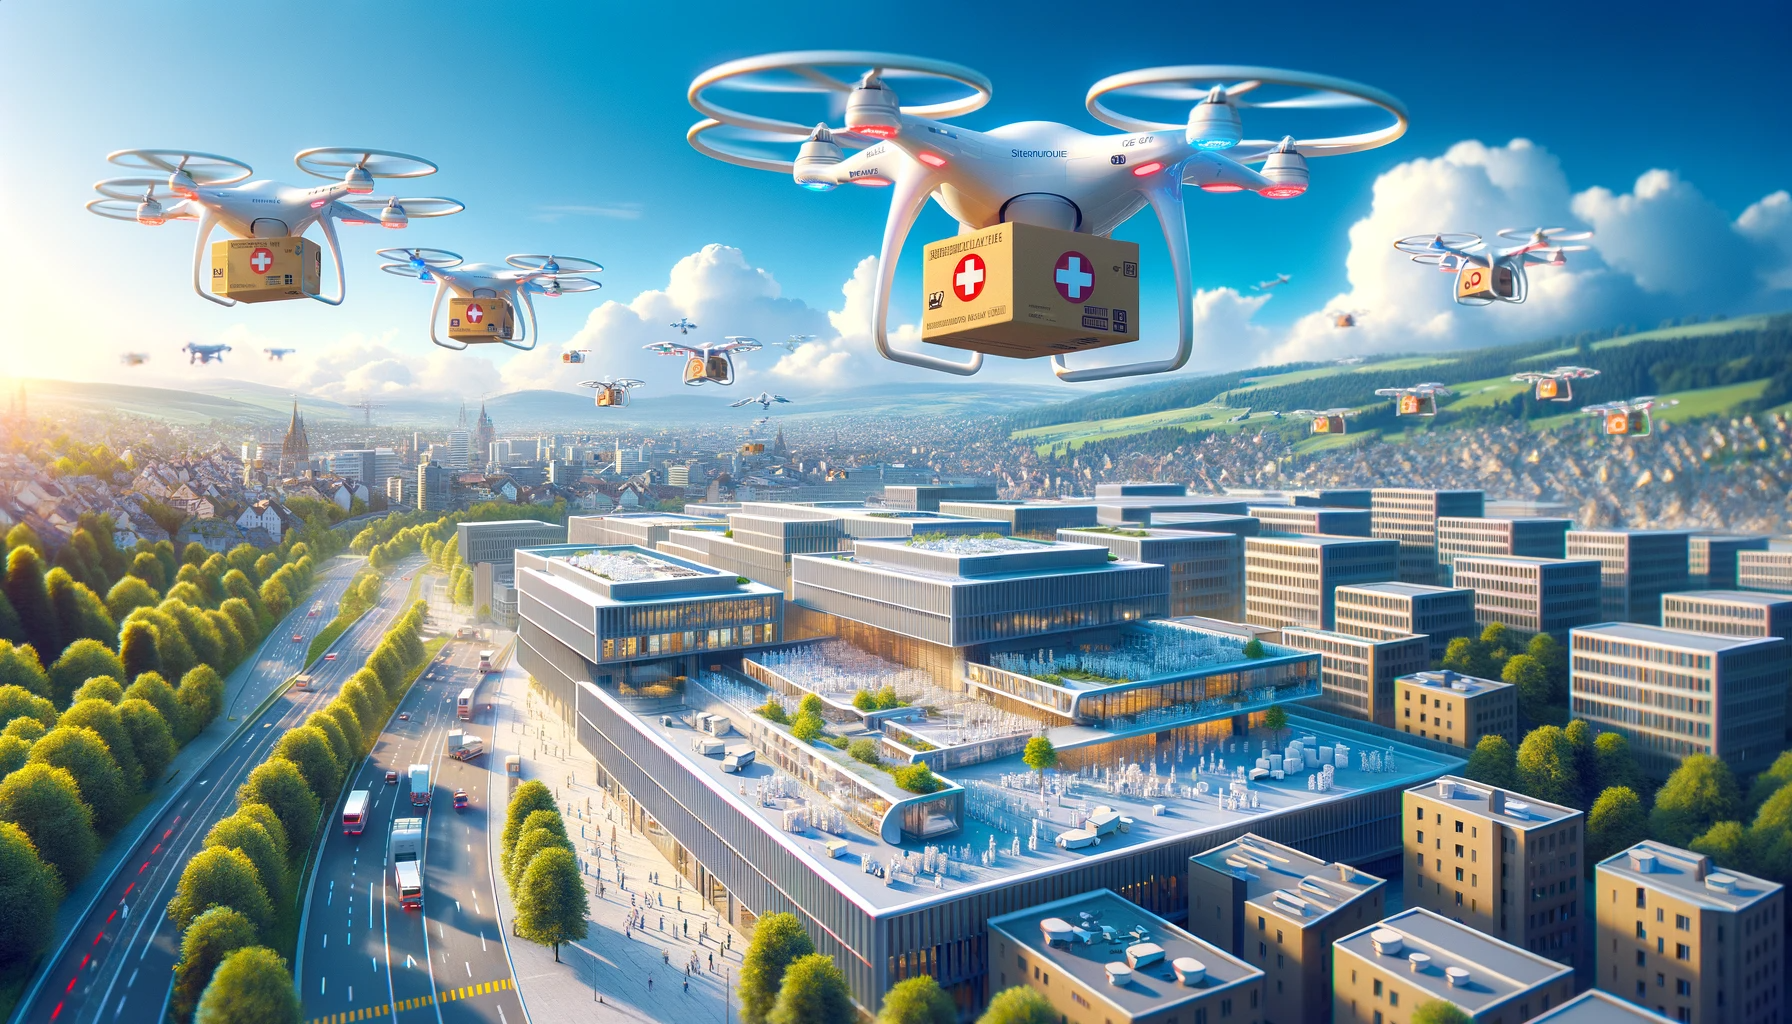
\includegraphics[width=0.85\textwidth]{./images/cover-image.png}
  \linebreak
  \linebreak
  \linebreak
  \linebreak
  \linebreak
  \linebreak
  \linebreak
  \linebreak
  \linebreak
  \linebreak
  \linebreak
  \linebreak
  \linebreak
  \linebreak
  \linebreak
  \linebreak
  \linebreak
  \linebreak
  \linebreak
  \linebreak
  \linebreak
  \linebreak
  \subsubtitlesize{\textbf{Version: \version}}
  \linebreak
  \linebreak
  \subsubtitlesize{\textbf{Execution period:} 13.12.2023 - 20.03.2024}
  \linebreak
  \begin{multicols}{2}
    \noindent\begin{minipage}[t][.3\textheight][t]{\columnwidth}
      \begin{flushright}
        \subsubtitlesize{\textbf{Responsible expert}}\hspace*{1cm}
        \linebreak
        \subsubtitlesize{\expert}\hspace*{1cm}
        \linebreak
        \subsubtitlesize{olga.samuel@sbl.ch}\hspace*{1cm}
        \linebreak
        \linebreak
        \subsubtitlesize{\textbf{Student}}\hspace*{1cm}
        \linebreak
        \subsubtitlesize{\fabian}\hspace*{1cm}
        \linebreak
        \subsubtitlesize{e036696@edu.sbl.ch}\hspace*{1cm}
        \linebreak
        \linebreak
        \subsubtitlesize{\textbf{Student}}\hspace*{1cm}
        \linebreak
        \subsubtitlesize{\xenia}\hspace*{1cm}
        \linebreak
        \subsubtitlesize{e036176@edu.sbl.ch}\hspace*{1cm}
      \end{flushright}
    \end{minipage}

    \columnbreak

    \noindent\begin{minipage}[t][.3\textheight][t]{\columnwidth}
      \begin{flushleft}
        \hspace*{1cm}\subsubtitlesize{\textbf{Student}}
        \linebreak
        \hspace*{1cm}\subsubtitlesize{\celine}
        \linebreak
        \hspace*{1cm}\subsubtitlesize{e036180@edu.sbl.ch}
        \linebreak
        \linebreak
        \hspace*{1cm}\subsubtitlesize{\textbf{Student}}
        \linebreak
        \hspace*{1cm}\subsubtitlesize{\jonas}
        \linebreak
        \hspace*{1cm}\subsubtitlesize{e036708@edu.sbl.ch}
      \end{flushleft}
    \end{minipage}
  \end{multicols}
\end{titlepage}

  \frontmatter
  \pagenumbering{Roman}
  \setcounter{page}{1}
\chapter*{Dokumentmanagement}
\vspace{-3cm}
\begin{table}[htp]
  \begin{tabularx}{\textwidth}{l X}
  Autor: & Jonas Schultheiss \\
  Version: & \version \\
  Datum: & \docdate \\
  Status: & Done \\
  Dateiname: & \compiledfilename \\
  \end{tabularx}
\end{table}

\begin{table}[htp]
  \begin{tabularx}{\textwidth}{l l X}\hline \\
  \textbf{Version} & \textbf{Datum} & \textbf{Änderung} \\ \\\hline \\
  0.0.1 & 29.03.2021 & Initialisierung des Dokuments \\
  0.0.2 & 29.03.2021 & Projektmanagementmethode beschrieben \\
  0.0.3 & 29.03.2021 & Systembeschreibung abgeschlossen \\
  0.0.4 & 30.03.2021 & Ist/Soll-Vergleich \\
  0.0.5 & 30.03.2021 & Namenskonzept \\
  0.0.6 & 30.03.2021 & Personas, Versionsverwaltungs- und Backupkonzept \\
  0.0.7 & 31.03.2021 & OAuth2 Strategie erstellt \\
  0.1.0 & 31.03.2021 & Analyse abgeschlossen \\
  0.1.1 & 31.03.2021 & Systementwurf begonnen \\
  0.1.2 & 01.04.2021 & Diagramme und Arbeitsjournale \\
  0.1.3 & 01.04.2021 & Systementwurf abgeschlossen \\
  0.1.4 & 01.04.2021 & Mockups erstellt und dokumentiert \\
  0.1.5 & 06.04.2021 & Testkonzept erarbeitet \\
  0.2.0 & 07.04.2021 & Entwurf finalisiert und Analyse korigiert  \\
  0.2.1 & 09.04.2021 & Implementation begonnen  \\
  \\\hline
  \end{tabularx}
\end{table}
\pagebreak
\begin{table}[htp]
  \begin{tabularx}{\textwidth}{l l X}\hline \\
  \textbf{Version} & \textbf{Datum} & \textbf{Änderung} \\ \\\hline \\
  0.3.0 & 13.04.2021 & Implementation fertiggestellt  \\
  0.3.1 & 13.04.2021 & Testing begonnen  \\
  0.4.0 & 13.04.2021 & Testing abgeschlossen  \\
  0.5.0 & 13.04.2021 & Abschluss erstellt  \\
  0.5.1 & 14.04.2021 & Glossar erstellt  \\
  0.5.2 & 14.04.2021 & Korrekturen einarbeitung begonnen\\
  1.0.0 & 14.04.2021 & Dokument fertiggestellt \\
  \\\hline
  \end{tabularx}
\end{table}

  \chapter*{Danksagung}
\vspace{-3cm}
Zunächst möchte ich Markus Strittmatter und Endress+Hauser für diese Ausbildung danken. Nur durch Sie konnte ich in den letzten vier Jahren meine Leidenschaft und mein Können für das Programmieren weiterentwickeln. Dafür bin ich froh, da ich nun weiss, dass Informatik das Richtige für mich ist. Es ist auch nicht selbstverständlich, einen Lehrling die Fachrichtung wechseln zu lassen. Dies erlaubte mir mich auch in der Schule voll und ganz auf das Programmieren zu fokussieren.
\newline
\newline
Gerne würde ich mich auch bei Valentino Rusconi und Marco Roth bedanken. Konnte ich etwas nicht alleine bewältigen, nahmen Sie sich die Zeit, um mir komplexe Konzepte zu erklären oder bei schwierigen Fehlern zu helfen.
\newline
\newline
Abschliessend möchte ich mich auch recht herzlich bei Lisa Marie Hüglin, Robert Kölblin und Simon Jäggi für das Korrekturlesen bedanken.
  \chapter*{Kurzfassung}
\vspace{-3.5cm}
\section*{Kurze Ausgangssituation}
\vspace{-0.2cm}
Die Endress+Hauser Gruppe verwendet Austellungsmodelle, um verschiedene Messgeräte aus dem eigenen Produktportfolio an Messen oder anderen offiziellen Anlässen vorzustellen. Die Messdaten der an den Modellen gezeigten Geräte können von den Kunden mittels dem IIoT Angebot \amk{Netilion} angezeigt und ausgewertet werden.
Ergänzend zu den durch Endress+Hauser angebotenen Standart Services, können Kunden zusätzlich eine Netilion Connect Subscription abschliessen. Eine solche Subscription erlaubt es dem Kunden auf die REST API der Netilion Cloud zuzugreifen, wodurch eigene Applikationen mit den Daten der Messgeräte erstellt werden können.
Um den Kunden die Möglichkeiten der Netilion Connect Subscription zu zeigen, wurde das \amk{OSE-Dashboard} erstellt. Dieses zeigt eine 3D Ansicht eines Austellungsmodells, das mittels Kameraführung betrachtet werden kann. Um zusätzliche Informationen über das dargestellte Modell zu zeigen, kann man mit den einzelnen Messgeräten interagieren, um beispielsweise deren aktuellen Status anzuzeigen.
Dieses Dashboard wurde statisch für ein bestimmtes Austellungsmodell in Reinach aufgebaut und ist nicht für andere Austellungsmodelle benutzbar. Damit entsteht die Problematik, dass bei Messen mit anderen Austellungsmodellen das Dashboard nicht gezeigt werden kann.

\vspace{-0.3cm}
\section*{Umsetzung}
\vspace{-0.2cm}

Um das Dashboard für alle weltweit verteilten Ausstellungsmodelle verwenden zu können, wurde mittels NextJS im Frontend und NestJS im Backend die Webapplikation erweitert. Zuerst wurden neue Entitäten in NestJS erstellt und bereits vorhandene angepasst. Anschliessend wurden die passenden Controller und Services erstellt, um dem Frontend eine Schnittstelle anbieten zu können. Dieses fragt Daten davon ab und visualisiert sie. Dadurch wurde eine Weltkarte, die Registrierung, das Konfigurationsmenü und die dynamische Darstellung des 3D Modells möglich.

\vspace{-0.3cm}
\section*{Ergebnis}
\vspace{-0.2cm}

Das Ergebnis ist ein erweitertes OSE Dashboard. Modellbetreiber auf der ganzen Welt können sich mittels OAuth2 anmelden und die eigenen Austellungsmodelle und deren Messgeräte erfassen. Somit kann das Dashboard dynamisch für alle Messen der Endress+Hauser Gruppe verwendet werden.
  \tableofcontents
  \mainmatter
  \pagestyle{fancy}
  \part{Obligatorische Kapitel}
  \chapter{Obligatorische Dokumentation}
\section{Ausgangslage}

In der Endress+Hauser Gruppe gibt es ein Messemodell mit dem Namen One Story Exhibit (OSE Modell). Dieses OSE Modell gibt es mehrfach in der gleichen Ausführung. Diese Modelle sind weltweit in den Endress+Hauser Sales Center verteilt. Dieses Modell bietet einen interaktiven Einblick in das Produkt Portfolio von Endress+Hauser Digital Solutions. Der Kunde kann unter anderem unser IIOT Angebot Netilion interaktiv erleben. Aktuell werden dafür unsere Netilion Standard Services wie z.B. Analytics, Health und Value verwendet. Dabei werden die Daten der Messgeräte via Edge Device in unserer IIOT Cloud gespeichert. Via Netilion Standard Web Applikationen kann man z.B. den aktuellen Health Status der Messgeräte sowie den aktuellen Messwert sehen.
\newline
\newline
Die Web Applikation „OSE Dashboard“ soll dem Kunden ein Beispiel für die Verwendung der Netilion Connect Subscription zeigen. Mit einer Netilion Connect Subscription erhält der Kunde Zugriff auf die REST API unserer Netilion Cloud und kann somit eigene IIOT Anwendungen entwickeln oder die Daten aus Netilion in seine eigene Cloud importieren. Die Applikation „OSE Dashboard“ zeigt das OSE Modell in einer 3D Ansicht. Man kann über eine Kameraführung an die Messgeräte heran zoomen und den Health Status des Messgerätes anzeigen lassen. Aktuell ist die Applikation nur mit dem OSE Modell in Reinach nutzbar, weil die Applikation nur mit den Daten der Messgeräte dieses Modells in Netilion verlinkt ist.
\newline
Mit dieser IPA soll die Web Applikation „OSE Dashboard“ so erweitert werden, dass sie für andere OSE Modelle mit gleichem Aufbau verwendet werden kann.
\section{Detaillierte Aufgabenstellung}

Die bestehende Web Anwendung „OSE Dashboard“ zeigt das One Story Exhibit Model (OSE Modell), welches in Reinach steht, in einer 3D Ansicht an. Darin werden die Daten der Messgeräte aus der Netilion Cloud gelesen und ebenfalls dargestellt.
\newline
Das Ziel dieses Projekts ist, dass die Web Anwendung auch für andere OSE Modelle, welche dem gleichen Aufbau haben, verwendet werden kann, ohne dass zukünftig eine Änderung an der Applikation notwendig ist.
\newline
Die bestehende Anwendung muss dafür so erweitert werden, dass Verlinkung des 3D Modells mit den Daten der Messgeräte nicht mehr im Source Code hinterlegt ist. Es muss ein Weg gefunden werden, diese Verlinkung für alle bestehenden und zukünftigen OSE Modelle zu speichern.
\newline
Laut Autraggeber haben alle OSE Modelle den gleichen Aufbau mit Messgeräten vom gleichen Typ. Auch die Bezeichnung der Messgeräte sollte bei allen Modellen gleich sein. Wird die Anwendung das erste mal für ein OSE Modell verwendet, muss für alle Geräte aus diesem OSE Modell die Verlinkung mit dem 3D Modell der Anwendung automatisch erfolgen und gespeichert werden. Sollte es aber Messgeräte geben, die nicht vom gleichen Typ sind, weil sie z.B. durch eine neuere Version ersetzt wurden, dann soll der Anwender die Möglichkeit haben über ein Konfigurationsmenü die Verlinkung vorzunehmen.
\newline
Änderungen an der Konfiguration dürfen nicht von jedem User vorgenommen werden. Das Konfigurationsmenü darf nur von Usern geöffnet werden, welche die entsprechende Berechtigung haben. Dafür soll in Netilion eine User Gruppe erstellt werden. Alle User dieser Gruppe dürfen dann die Konfiguration ändern.
\newline
Die Anwendung selber soll aber weiterhin ohne Login aufrufbar sein. Der Anwender soll als Datenquelle für das 3D Modell zwischen den verschiedenen integrierten Standorten wählen können. Da jedes OSE Modell einen eigenen User hat, müssen die User Credentials der einzelnen OSE Modelle ebenfalls in der Applikation gespeichert werden. Dabei muss darauf geachtet werden, dass diese Daten sicher gespeichert werden und der Anwender keinen Zugriff darauf hat.
\newline
Die Methoden mit der Logik für die automatische Verlinkung der Messgeräte mit dem 3D Modell soll automatisiert getestet werden.
\newline
Für den Test der kompletten Applikation sind manuelle Tests ausreichend. Dabei sind folgende Testsfälle zu beachten:
\begin{itemize}
  \item Konfigurationsmenu nur mit entsprechender Berechtigung aufrufbar
  \item Alle Messgeräte werden automatisch verlinkt.
  \item Messgeräte können nicht automatisch verlinkt werden .
  \item User kann ohne Login zwischen integrierten OSE Modellen wechseln.
  \item Credentials der OSE Modelle sind sicher gespeichert
\end{itemize}
Die Tests sollen zuerst an dem OSE Modell in Reinach durchgeführt werden. Bei diesem Modell können auch für Tests die Daten in Netilion mal abgeändert werden.
Zum Abschluss sollen 2 weitere OSE Modelle integriert werden um die funktionalität der Anwendung mit mehreren OSE Modellen zu testen.

\pagebreak
\section{Mittel und Methoden}
Anbei werden Mittel und Methoden aufgelistet, welche von diese IPA gefordert werden:
\begin{itemize}
  \item HTML \& CSS
  \item JavaScript
  \item Node.js JavaScript Runtime Environment für Desktop und Server
  \item React Eine von FaceBook entwickelte JavaScript Bibliothek, welche die Strukturierung von Komponenten basierten Benutzeroberflächen erleichtert.
  \item JSX Ein Syntax welcher das übliche JavaScript erweitert. Es ermöglicht das Vermischen von HTML mit JavaScript und wird
  von React verwendet
  \item Three JavaScript Bibliothek, welche es ermöglicht 3D Modelle in einem HTML Canvas darzustellen
  \item react-three-fiber JavaScript Bibliothek, welche auf Three aufbaut und das ganze in React verfügbar macht
  \item GLTF Dateiformat für 3D Modelle, welches sich am besten für das Web eignet
\end{itemize}

Hosting der Web Applikation
\begin{itemize}
  \item Heroku
  \item Vercel
\end{itemize}

Entwicklungsumgebung
\begin{itemize}
  \item Macbook Pro 2018 mit Dockingstation und 2 externen Monitoren. (Ersatzweise steht ein Windows Laptop zur Verfügung)
  \item MacOS Big Sur
  \item Visual Studio Code
  \item GitHub
\end{itemize}

\section{Vorkenntnisse}
Alle Tools und Techniken sind dem Lernenden schon bekannt. Er hat alle Tools, Programmiersprachen und Techniken schon in mehreren Projekten während der Ausbildung angewendet.

\section{Vorarbeiten}
Die Version 1 des OSE Dashboards wurde als Vorarbeit zu dieser IPA vom Lernenden entwickelt.

\section{Neue Lerninhalte}
In dieser IPA gibt es keine neuen Lerninhalte.

\section{Arbeiten in den letzten sechs Monaten}
Entwickeln einer Webanwendung, welche Daten aus der Endress+Hauser IIOT Plattform Netilion darstellt. Diese Anwendung zeigt den Wasserverbrauch der Kaffeemaschinen in der Pausenzone an und berechnet die Anzahl der konsumierten Tassen. Diese Anwendung dient dazu, unseren Kunden das Angebot Netilion Connect zu erklären.
\newline
Entwickeln einer weiteren Webanwendung, welche in Verbindung mit Netilion Connect Daten aus der Endress+Hauser IIOT Plattform darstellt. Dies ist die erste Version des OSE Dashboards, welches ein Messemodell in 3D darstellt und den „Gesundheitszustand“ der Messgeräte anzeigt. Diese Webanwendung wird im Rahmen dieser IPA erweitert.
\section{Projektaufbauorganisation}

\begin{figure}[!ht]
  \centering
  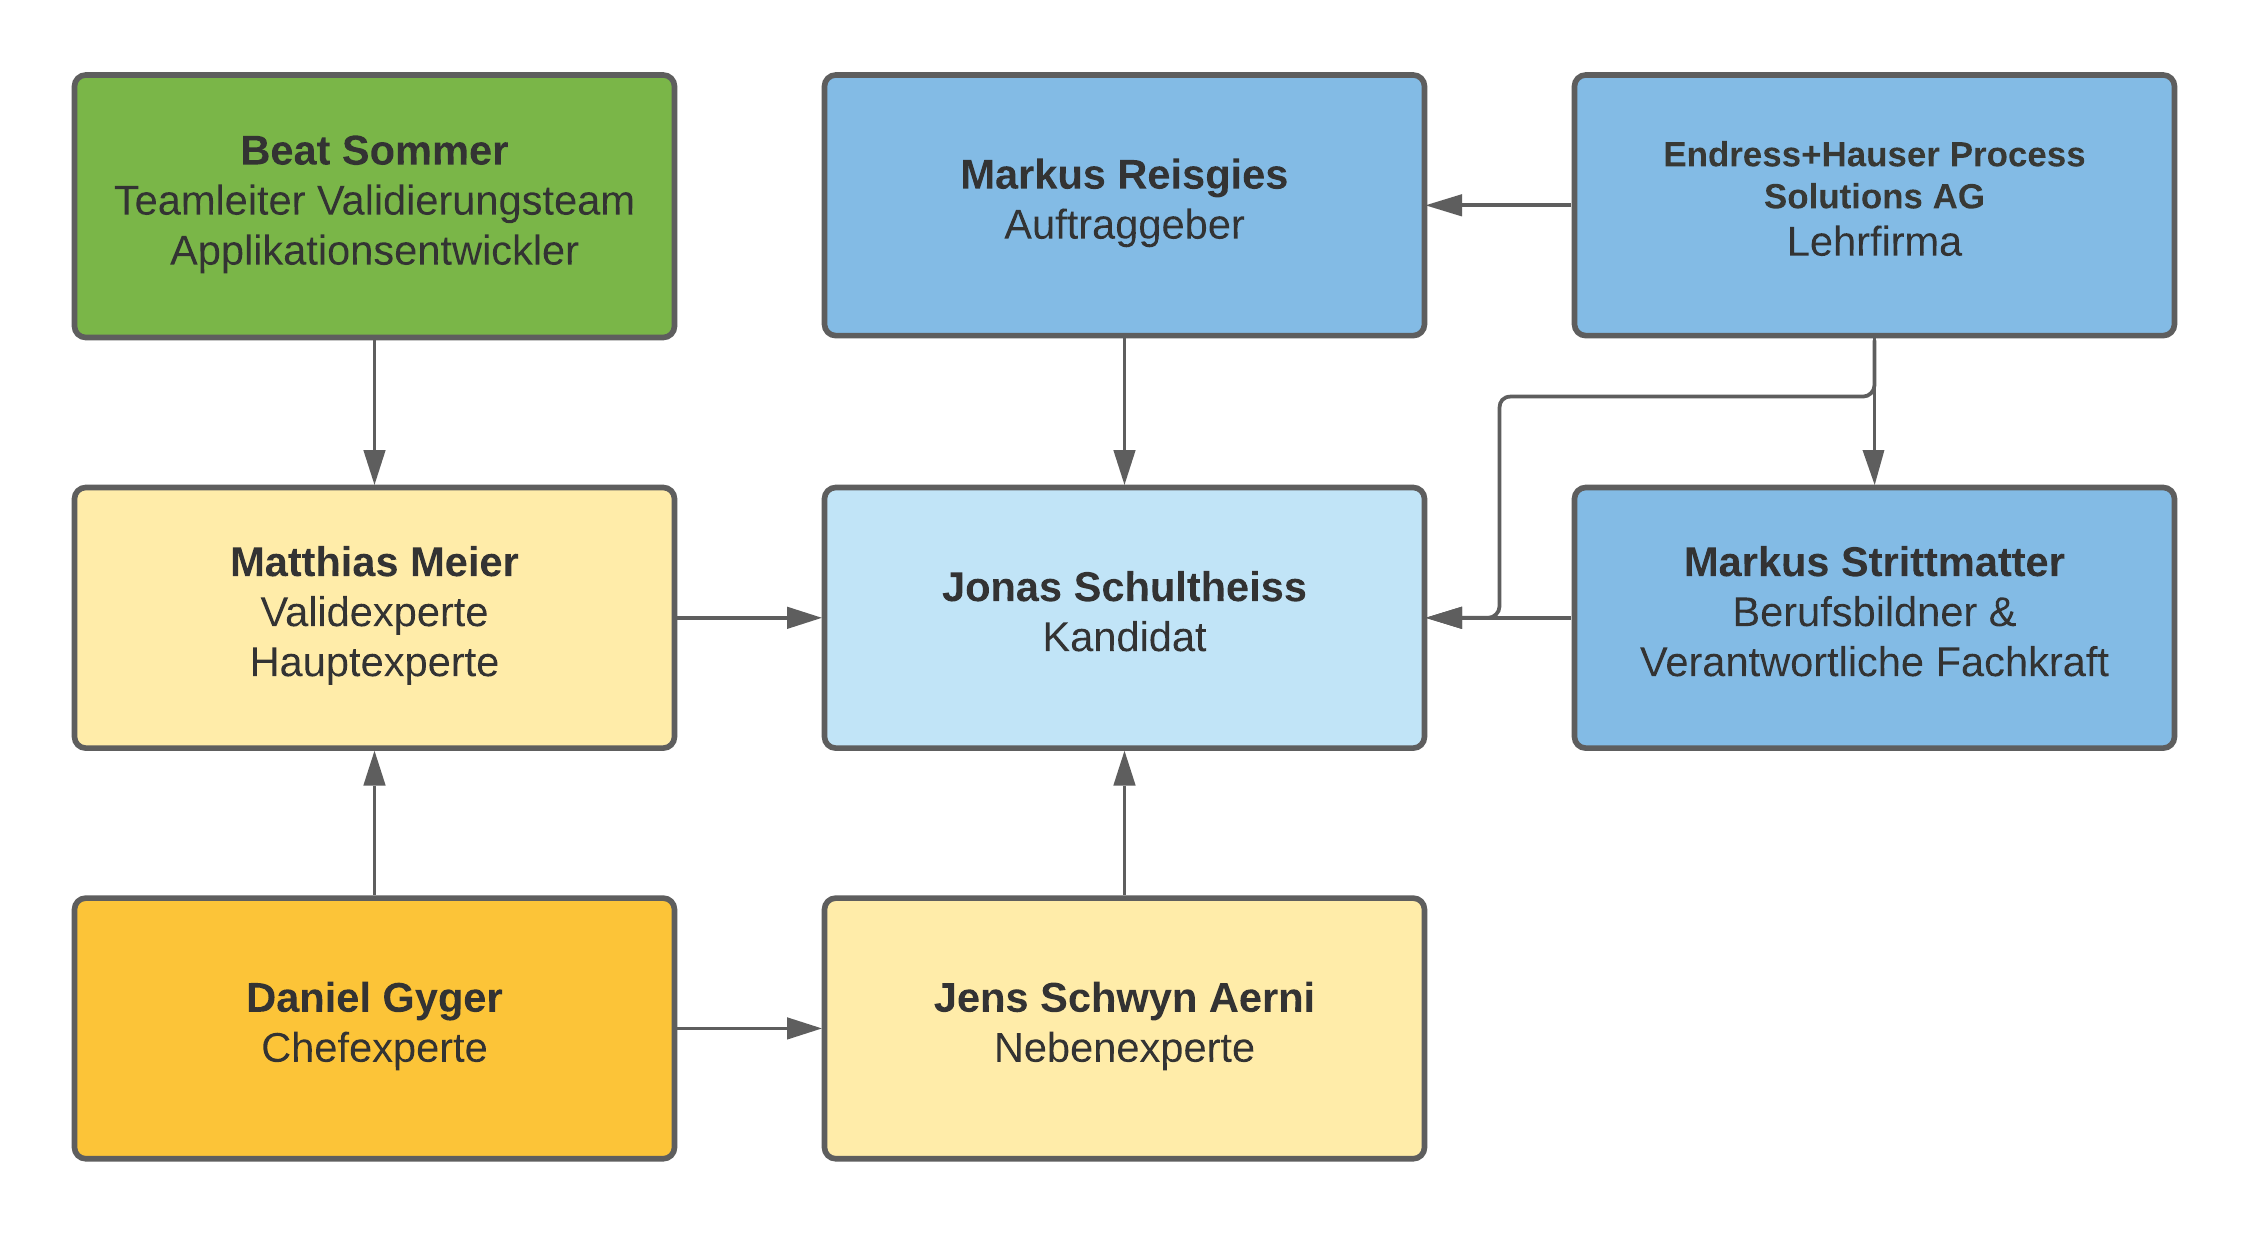
\includegraphics[width=.95\linewidth]{./images/Projektaufbauorganisation.png}
  \caption[Diagram der Projektaufbauorganisation]{Diagram der Projektaufbauorganisation}
  \label{fig:projektaufbauorganisation}
\end{figure}
\pagebreak
\section{Durchführungsblock}

\begin{table}[htp]
  \begin{tabularx}{\textwidth}{l X}
    Startblock 2: & 29.03.2021 – 16.04.2021\\
    PA-Durchführung: & 29.03.2021 – 14.05.2021 \\
    Einreichung bis: & 31.01.2021 \\
  \end{tabularx}
\end{table}

\section{IPA-Termine}

\begin{table}[htp]
  \begin{tabularx}{\textwidth}{l X}
    Antrittsgespräch: & 23.03.2021 08:30 \\
    Erster Zwischenbesuch: & 01.04.2021 09:00 \\
    Zweiter Zwischenbesuch: & 08.04.2021 09:45 \\
    Endbesuch: & 28.04.2021 09:00 \\
  \end{tabularx}
\end{table}
\newpage
\section{Projektplan}
\pdfpagewidth= 2\paperwidth
\begin{addmargin}[0pt]{-\paperwidth}
    \begin{figure}[!h]
          \centering
        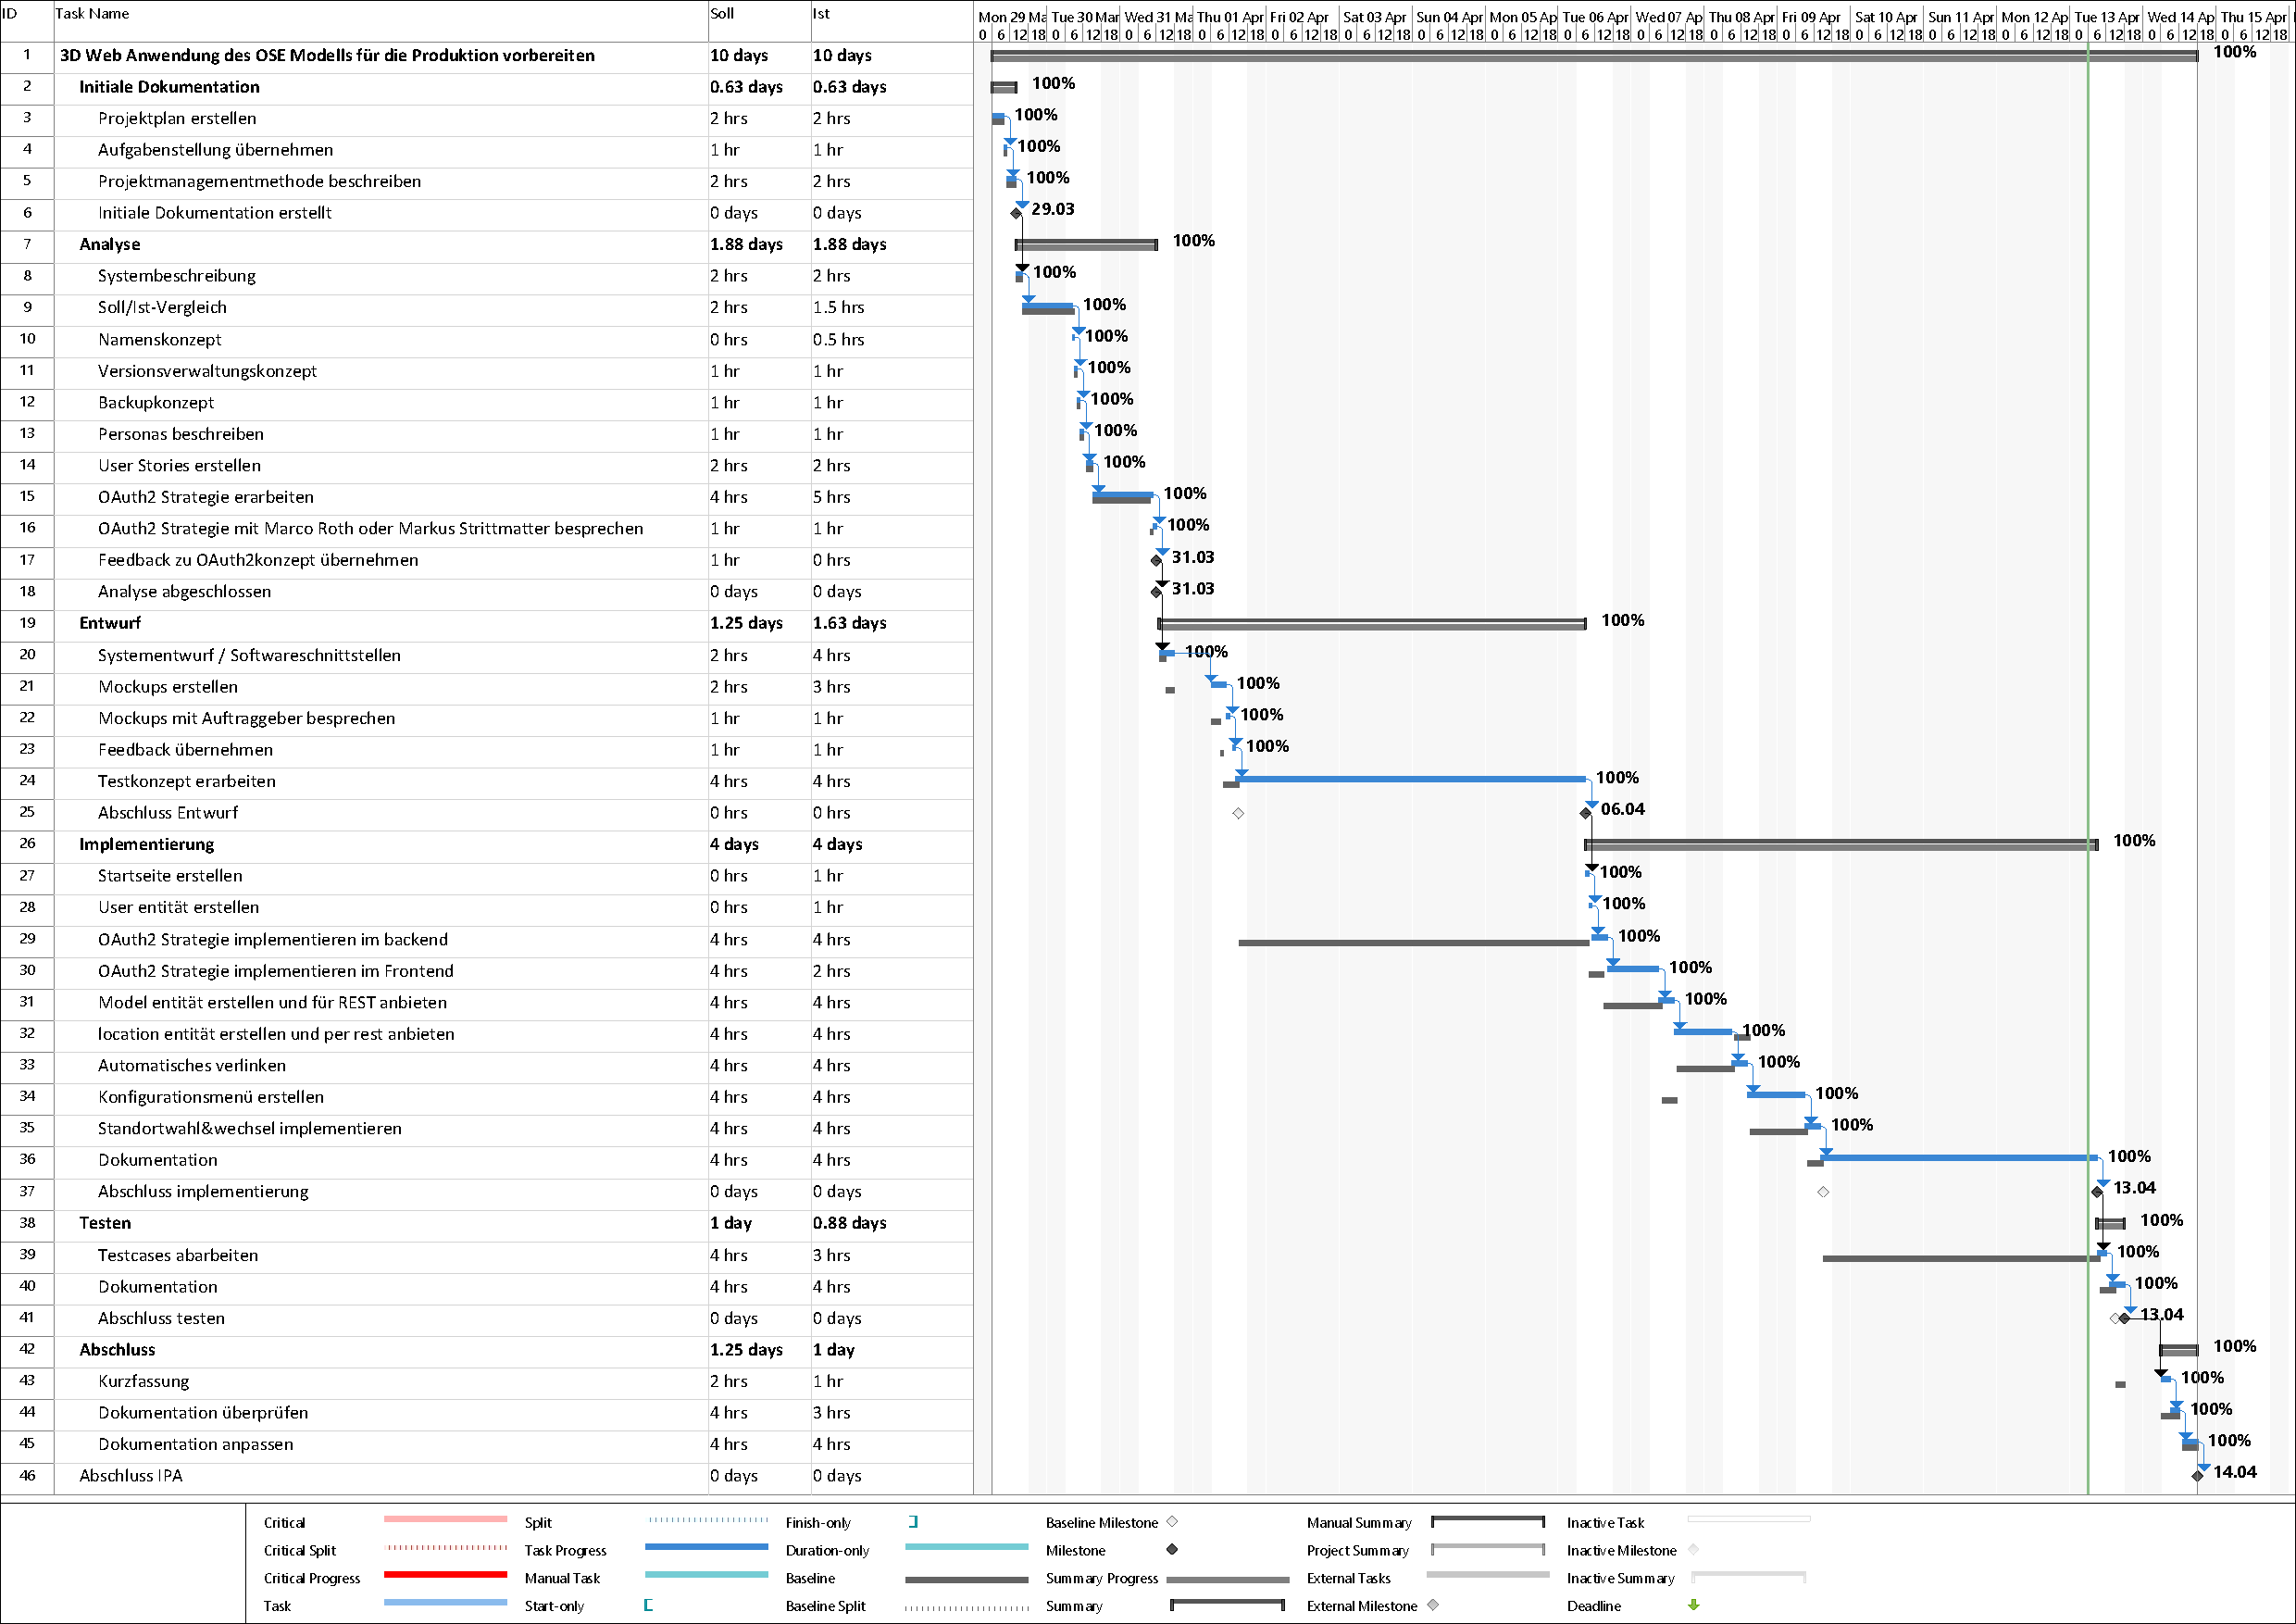
\includegraphics[height=0.85\textheight]{./projektplan/projektplan_ipa_a3.pdf}
        \caption[{Projektplan, erstellt mit Microsoft Projekts}]{Projektplan, erstellt mit Microsoft Projekts}
    \end{figure}
\end{addmargin}
\newpage
\pdfpagewidth= \paperwidth
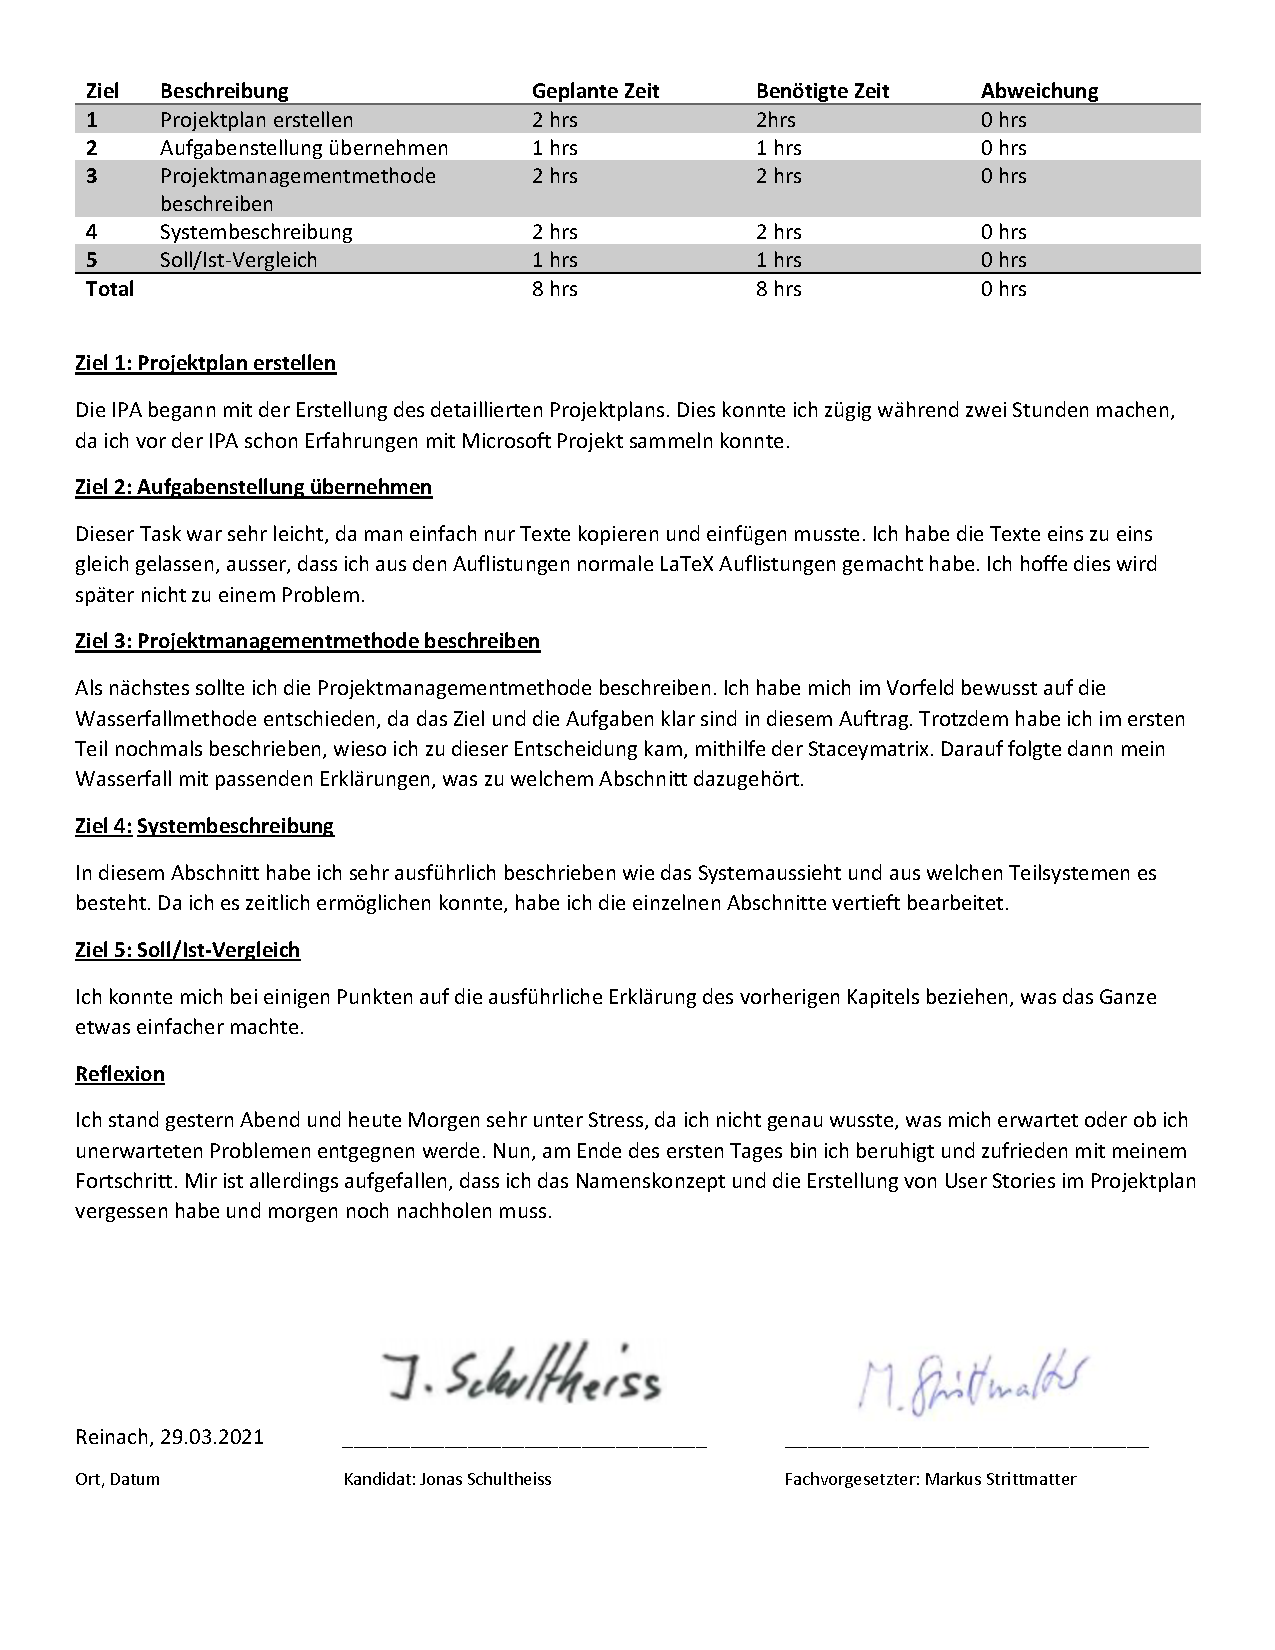
\includepdf[pages={1},pagecommand=\section{Arbeitsjournale}\subsection{Arbeitsjournal vom 29.03.2021},width=\textwidth, scale=0.9]{./arbeitsjournal/Arbeitsjournale.pdf}
\includepdf[pages={2},pagecommand=\subsection{Arbeitsjournal vom 30.03.2021},width=\textwidth, scale=0.9]{./arbeitsjournal/Arbeitsjournale.pdf}
\includepdf[pages={3},pagecommand=\subsection{Arbeitsjournal vom 31.03.2021},width=\textwidth, scale=0.9]{./arbeitsjournal/Arbeitsjournale.pdf}
\includepdf[pages={4},pagecommand=\subsection{Arbeitsjournal vom 01.04.2021},width=\textwidth, scale=0.9]{./arbeitsjournal/Arbeitsjournale.pdf}
\includepdf[pages={5},pagecommand=\subsection{Arbeitsjournal vom 06.04.2021},width=\textwidth, scale=0.9]{./arbeitsjournal/Arbeitsjournale.pdf}
\includepdf[pages={6},pagecommand=\subsection{Arbeitsjournal vom 07.04.2021},width=\textwidth, scale=0.9]{./arbeitsjournal/Arbeitsjournale.pdf}
\includepdf[pages={7},pagecommand=\subsection{Arbeitsjournal vom 08.04.2021},width=\textwidth, scale=0.9]{./arbeitsjournal/Arbeitsjournale.pdf}
\includepdf[pages={8},pagecommand=\subsection{Arbeitsjournal vom 09.04.2021},width=\textwidth, scale=0.9]{./arbeitsjournal/Arbeitsjournale.pdf}
\includepdf[pages={9},pagecommand=\subsection{Arbeitsjournal vom 13.04.2021},width=\textwidth, scale=0.9]{./arbeitsjournal/Arbeitsjournale.pdf}
\includepdf[pages={10},pagecommand=\subsection{Arbeitsjournal vom 14.04.2021},width=\textwidth, scale=0.9]{./arbeitsjournal/Arbeitsjournale.pdf}
  \part{Dokumentation}
  \chapter{Projektmanagement}
\section{Entscheidung}
Die Entscheidung der Projektmanagementmethode ist sehr wichtig und sollte sorgfältig gemacht werden. Sollte eine Methode falsch angewandt werden, kann sie das Team verlangsamen und bei der Arbeit hindern. Bei dieser Entscheidung hilft die Stacey Matrix.

\begin{wrapfigure}[15]{r}[0pt]{0.5\textwidth}
  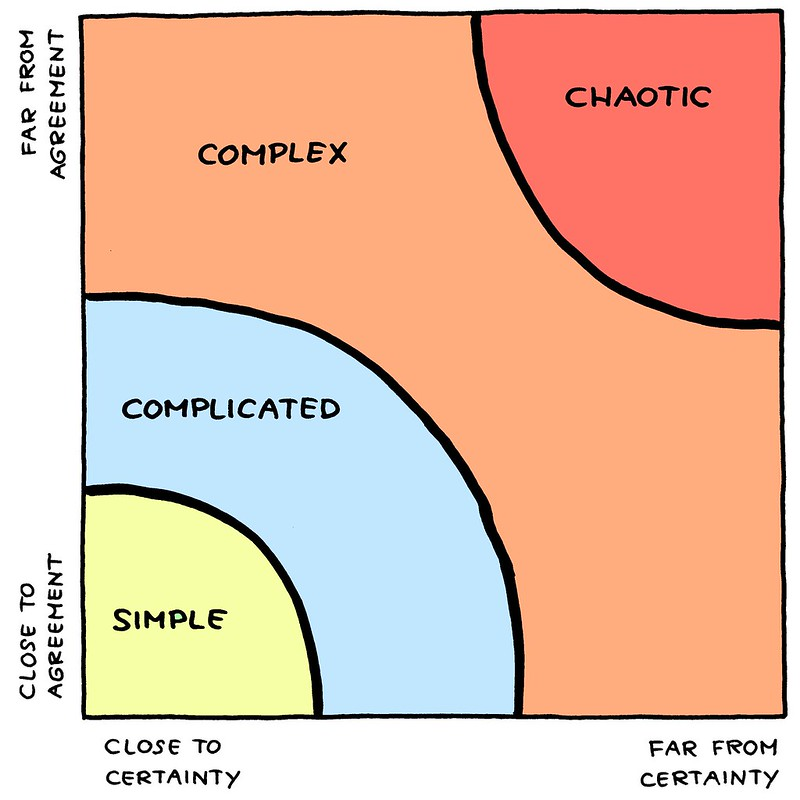
\includegraphics[width=0.9\linewidth]{./images/stacey_matrix}
  \caption[\href{https://blog.ordix.de/welches-vorgehen-eignet-sich-fuer-mein-projekt}{Stacey Matrix Grafik von Jurgen Appello.}]{Stacey Matrix}
  \label{fig:stacey}
\end{wrapfigure}\leavevmode

Die x-Achse beschreibt die Verständlichkeit des Auftrags. Das heisst, ob alle Anforderungen gegeben sind oder noch welche zu einem späteren Zeitpunkt dazu kommen können. Die y-Achse beschreibt dagegen, wie deutlich der Weg zu diesen Anforderungen ist. Dabei fragt sich zum Beispiel, wie man den Auftrag mit dieser Programmiersprache lösen kann.
\newline
Die ganze Auswertung beruht auf Schätzungen. Diese subjektiven Beobachtungen werden allerdings präziser, je mehr Berufserfahrung man sammelt.
\newline
In der Abbildung \ref*{fig:stacey} gibt es vier Abschnitte. Je Kategorie sollte man eine andere Projektmanagementmethode anwenden.
\newpage
\begin{itemize}
  \item \textbf{Simpel} - Das Ziel und der Weg sind klar. In diesem Fall sollte das Wasserfallmodell oder eine ähnliche Methode gewählt werden.
  \item \textbf{Kompliziert} - Sollte entweder das Ziel oder noch nicht ganz klar sein, sollte man Kanban anwenden.
  \item \textbf{Komplex} - Sind beide Achsen unklar oder ändern sich Kriterien, sollte etwas Agiles wie Scrum gewählt werden. Eine Methode wie diese  eignet sich für wechselnde Anforderungen.
  \item \textbf{Chaotisch} - Das Ziel und der Weg sind unklar. In diesem Fall sollte das Projekt noch nicht gestartet werden. Stattdessen sollte für mehr Klarheit bezüglich Weg und Ziel geschaffen werden. 
\end{itemize}

\section{Wasserfallmodell}

\begin{figure}[!ht]
  \centering
  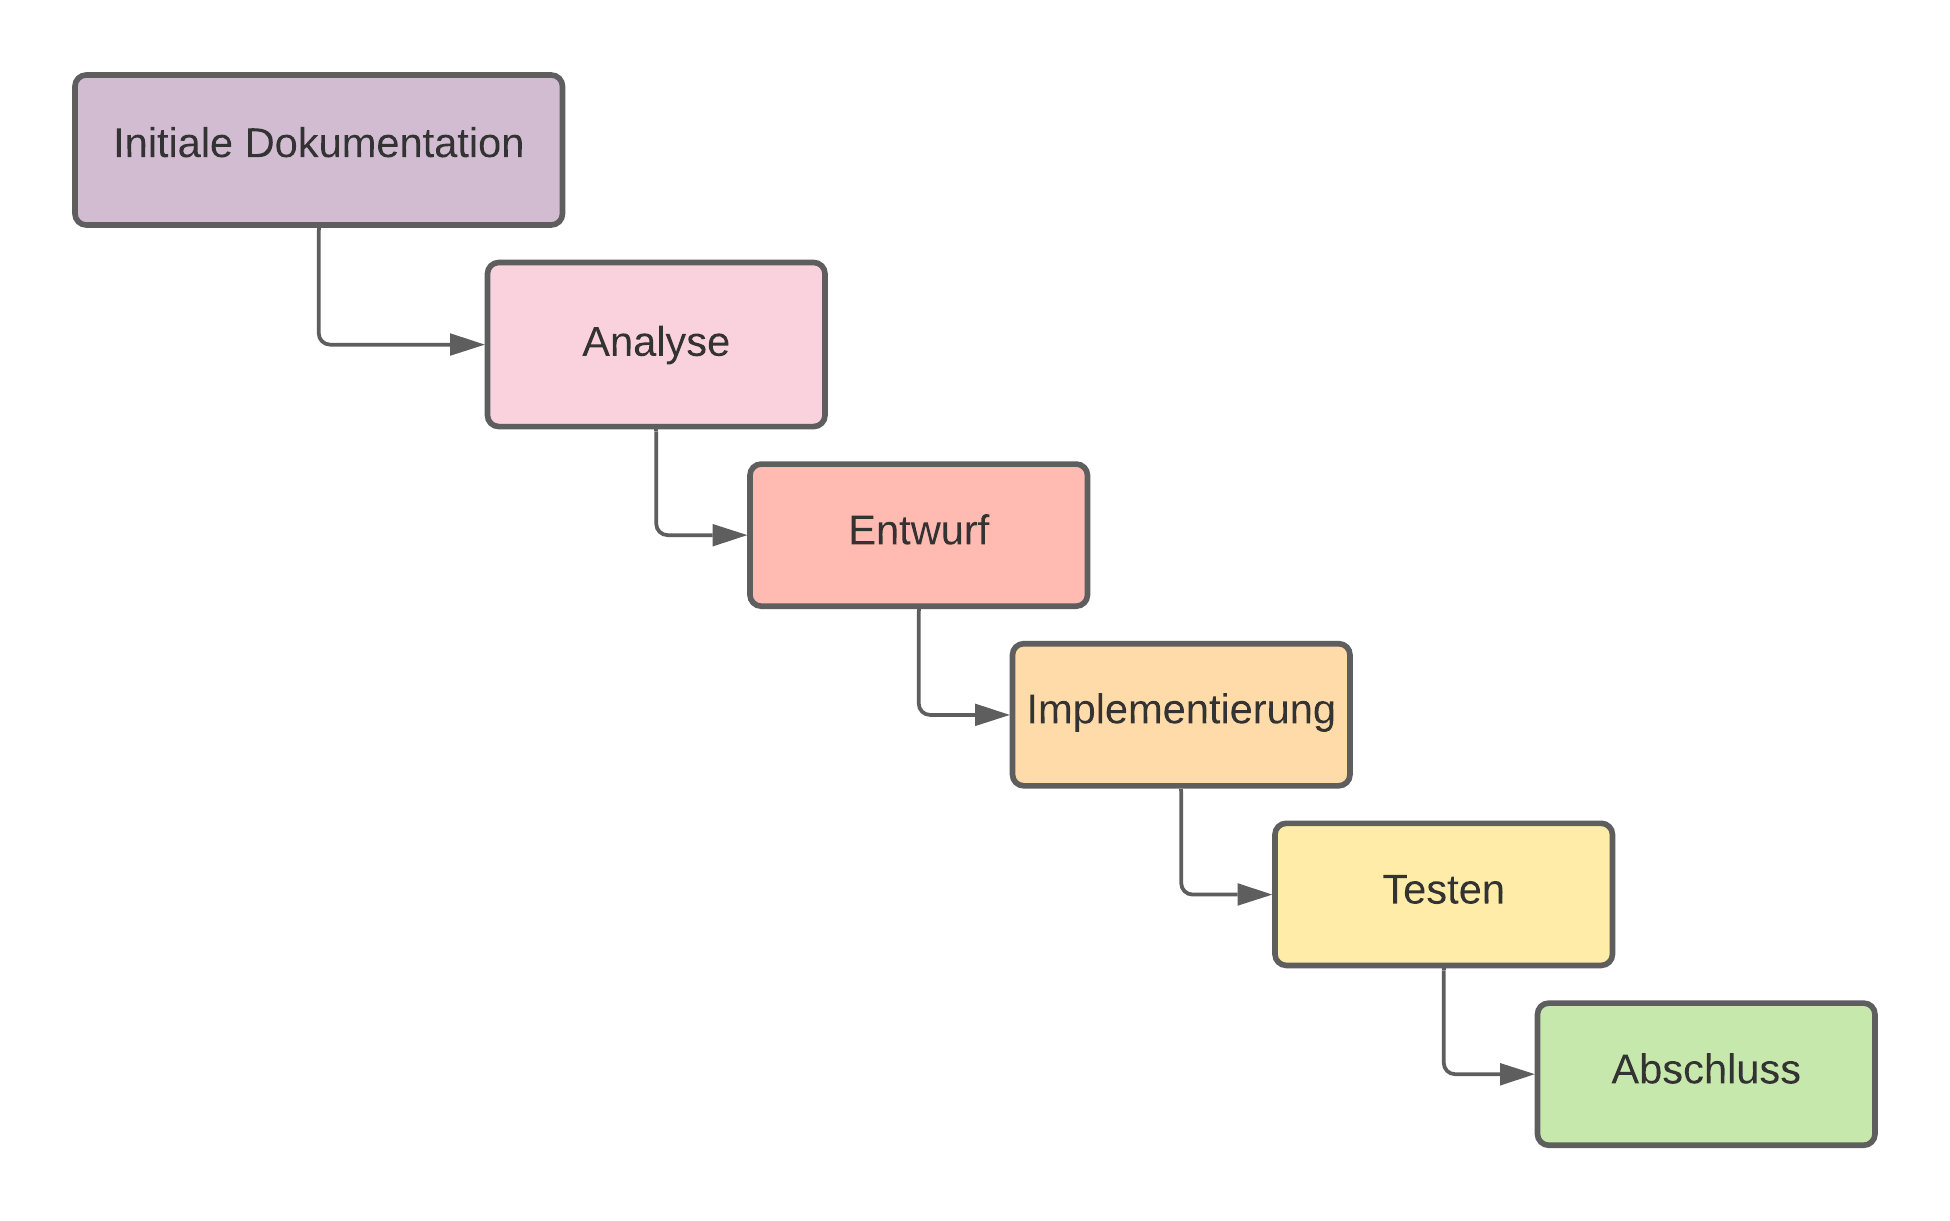
\includegraphics[width=.95\linewidth]{./images/OSEDashboard_Wasserfall.png}
  \caption[Ein von mir mit Lucidchart erstelltes Wasserfallmodell]{Wasserfall Modell}
  \label{fig:wasserfall}
\end{figure}

Das Wasserfallmodell ist eine Abfolge sequenzieller Phase, wobei man erst mit der nächsten Stufe beginnt, wenn die davorliegende abgeschlossen ist. Dies erfordert, dass das Ziel und der Weg klar sein muss. Ein streng geregelter Arbeitsablauf mit Meilensteinen kann dadurch ermöglicht werden, was vorallem für kleine Projekte sehr nützlich ist. Dies ist auch der Grund, weshalb man sich bei dieser Arbeit für das Wasserfallmodel entschieden hat.

\subsection{Initialisierung des Dokuments}

Als Erstes soll das Dokument für die kommenden Arbeitstage so vorbereitet werden, damit zukünftige zeitaufwendige Anpassungen vermeiden werden können. Zuerst soll die LaTeX-Vorlage nochmals angesehen werden, um sicherzugehen, dass alles stimmt und richtig konfiguriert ist. Danach sollten essenzielle Bestandteile wie der detaillierte Zeitplan, das Arbeitsjournal und der obligatorische Teil erstellt werden.

\subsection{Analyse}

Nachdem die Initialisierung komplett abgeschlossen ist, geht es an die Analyse. Diese beinhaltet unter Anderem eine Systembeschreibung, ein Ist/Soll-Vergleich, Konzepte wie die Arbeitsergebnisse gesichert werden und die OAuth2-Strategie. Ersteres beschreibt, wie genau unser Netilion-Ökosystem funktioniert und wie dieses Projekt integriert werden soll. Der Ist/Soll-Vergleich zeigt nochmals die zu erarbeitende Lösung auf und wie sie sich von dem bereits existierenden Produkt differenziert. Die OAuth2-Strategie soll genau beschreiben, wie der Anmeldeprozess abläuft und was ihn sicher macht.
\newline
Ausserdem enthalten sind Personas und detaillierte User-Stories. Diese werden gebildet, indem die Anforderung des Auftraggebers unterteilt werden, damit sich der Entwickler auf einzelne Entwicklungsabschnitte konzentrieren kann und der Fortschritt messbarer ist.

\subsubsection{User-Stories}

Die User Story beschreibt in kurzer Form eine Anforderung einer Anspruchsgruppe an die Software. Dabei soll geklärt werden, \textbf{wer} welche \textbf{Funktionalität} aus welchem \textbf{Grund} implementiert haben möchte\cite{atlassian_2021_user}. Ohne dabei zu sehr in technische Details zu gehen, beschreibt sie, was genau von der Software gefordert ist. Dadurch wird die Absprache mit den Anspruchsgruppen erleichter. Wie die Anforderungen implementiert werden, liegt im Ermessen des Entwicklers. Sehr oft wird diese kurze Beschreibung als Titel für eine Story im Projektmanagementtool angegeben.

\textbf{Beispiel einer User Story:}
\newline
\textbf{Aufbau:} Als \textit{<Anspruchsgruppe>} möchte ich \textit{<Feature>}, damit \textit{<Anwendungsfall>} erreicht wird.
\linebreak
\textbf{Beispiel:} Als \textit{Nutzer} möchte ich, dass \textit{die ne107 Werte grafisch dargestellt werden} , damit \textit{ich die Status der Messgeräte direkt sehen kann}.

\subsection{Entwurf}

In der Entwurfsphase wird der genaue Lösungsweg ermittelt. Der Entwickler beschreibt, wie er mit welchen technischen Mitteln die zuvor definierten Ziele erreichen kann. Dazu gehören Schnittstellen, Bibliotheken, Datenbank und Weiteres. Das Ergebnis dieser Phase ist ein ausgearbeitetes User Interface/User Experience Design, genaue Pläne, wie die Software aufgebaut werden soll und das Testkonzept.

\subsection{Implementierung}

In diesem Abschnitt gilt es, die dokumentierten Anforderungen mit den gewählten Technologien umzusetzen. Dabei sollen die User-Stories und Testfälle der vorherigen Kapiteln berüclsichtigt werden.
\newline
Nachdem eine Story abgeschlossen ist, wird die Änderung auf einen Branch gepusht und automatisch deployed. So können die Anspruchsgruppen dem Entwickler zeitnahe Rückmeldungen geben. Das Produkt der späteren Implementierungsphase ist die fertige Software.


\subsection{Testen}

In dieser Phase wird nochmals sorgfältig durchgegangen, ob alle Kriterien erfüllt wurden und ob die Tests wie gewünscht ablaufen. Stimmt das Ergebnis mit den gesetzten Erwartungen, gilt die Software als fertiggestellt.

\subsection{Abschluss}

Nachdem alle Ziele erreicht und mit dem Testprotokoll verifiziert wurden, wird die verbleibende Zeit für die Überarbeitung der Dokumentation eingesetzt werden. Anschliesend soll die IPA am 14.04.2021 abgegeben werden.

\chapter{Analyse}
\section{Systembeschreibung}
\subsection{Systemarchitektur}
\begin{figure}[!ht]
  \centering
  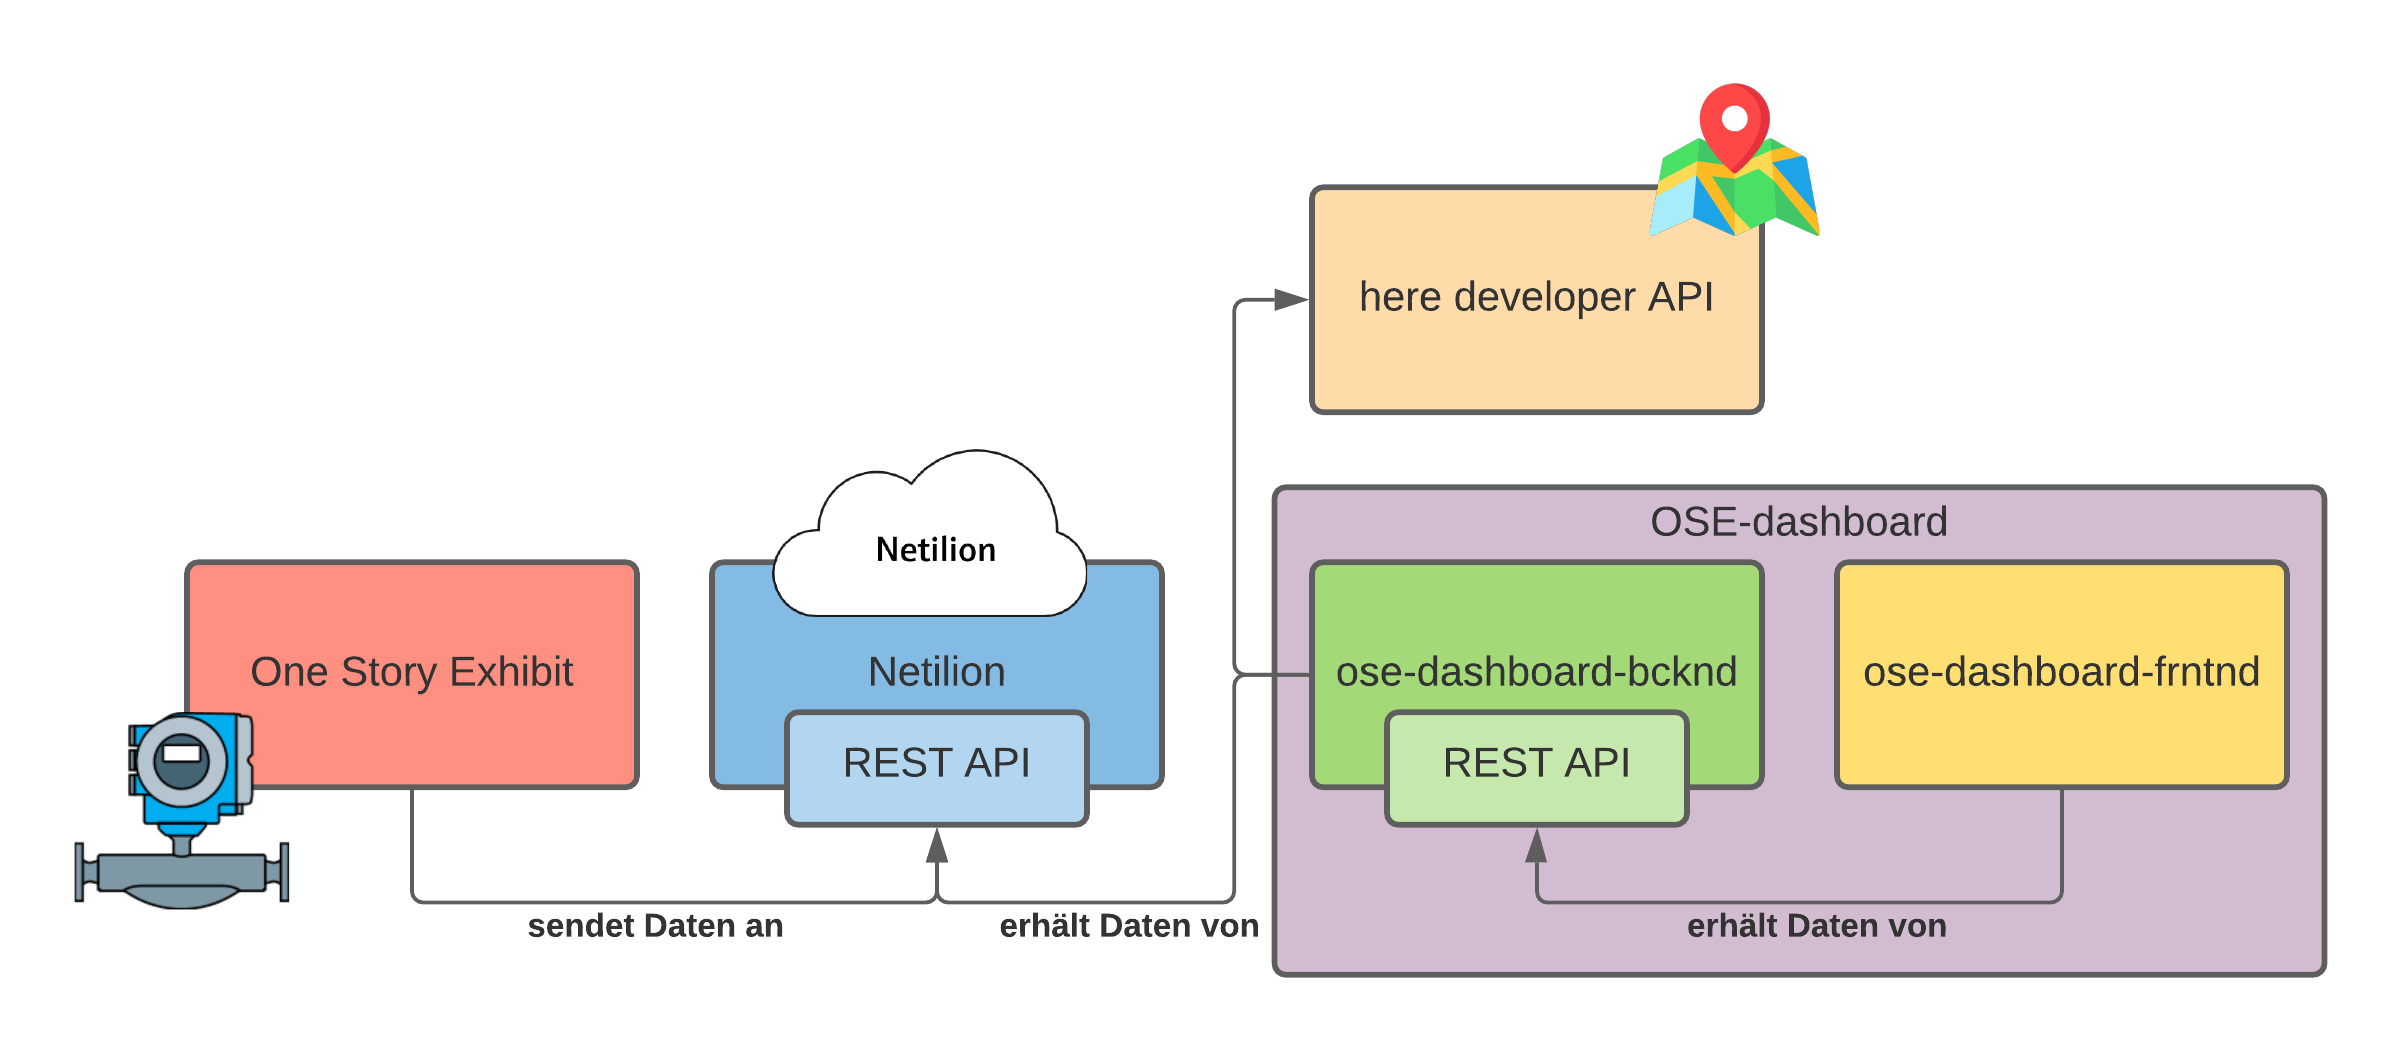
\includegraphics[width=1\linewidth]{./images/system.png}
  \caption[Eine von mir mit Lucidchart erstellte grobe Systemarchitektur]{Grobe Systemarchitektur}
  \label{fig:systemarchitektur}
\end{figure}
\cite{flaticon}
Das System des OSE-Dashboards besteht aktuell aus fünf essenziellen Teilen. Die Systemteile werden in den nachfolgenden Kapiteln \ref{arch-ose} bis \ref{arch-frontend} erläutert.
\subsection{One Story Exhibit} \label{arch-ose}
In diesem Projekt sollen die Anlagedaten der Endress+Hauser Ausstellungsmodelle von der Applikation ausgewertet werden. Endress+Hauser verwendet diese Modelle an Messen oder lokalen Vertriebsorganisationen, um den Kunden das umfassende Portfolio an Messgeräten näher zu bringen. Diese Applikation soll unterstützend demonstrieren, was mit dem IIoT Service \amk{Netilion} für Kunden möglich ist.
\subsection{Netilion} \label{arch-netilion}
\begin{figure}[!ht]
  \centering
  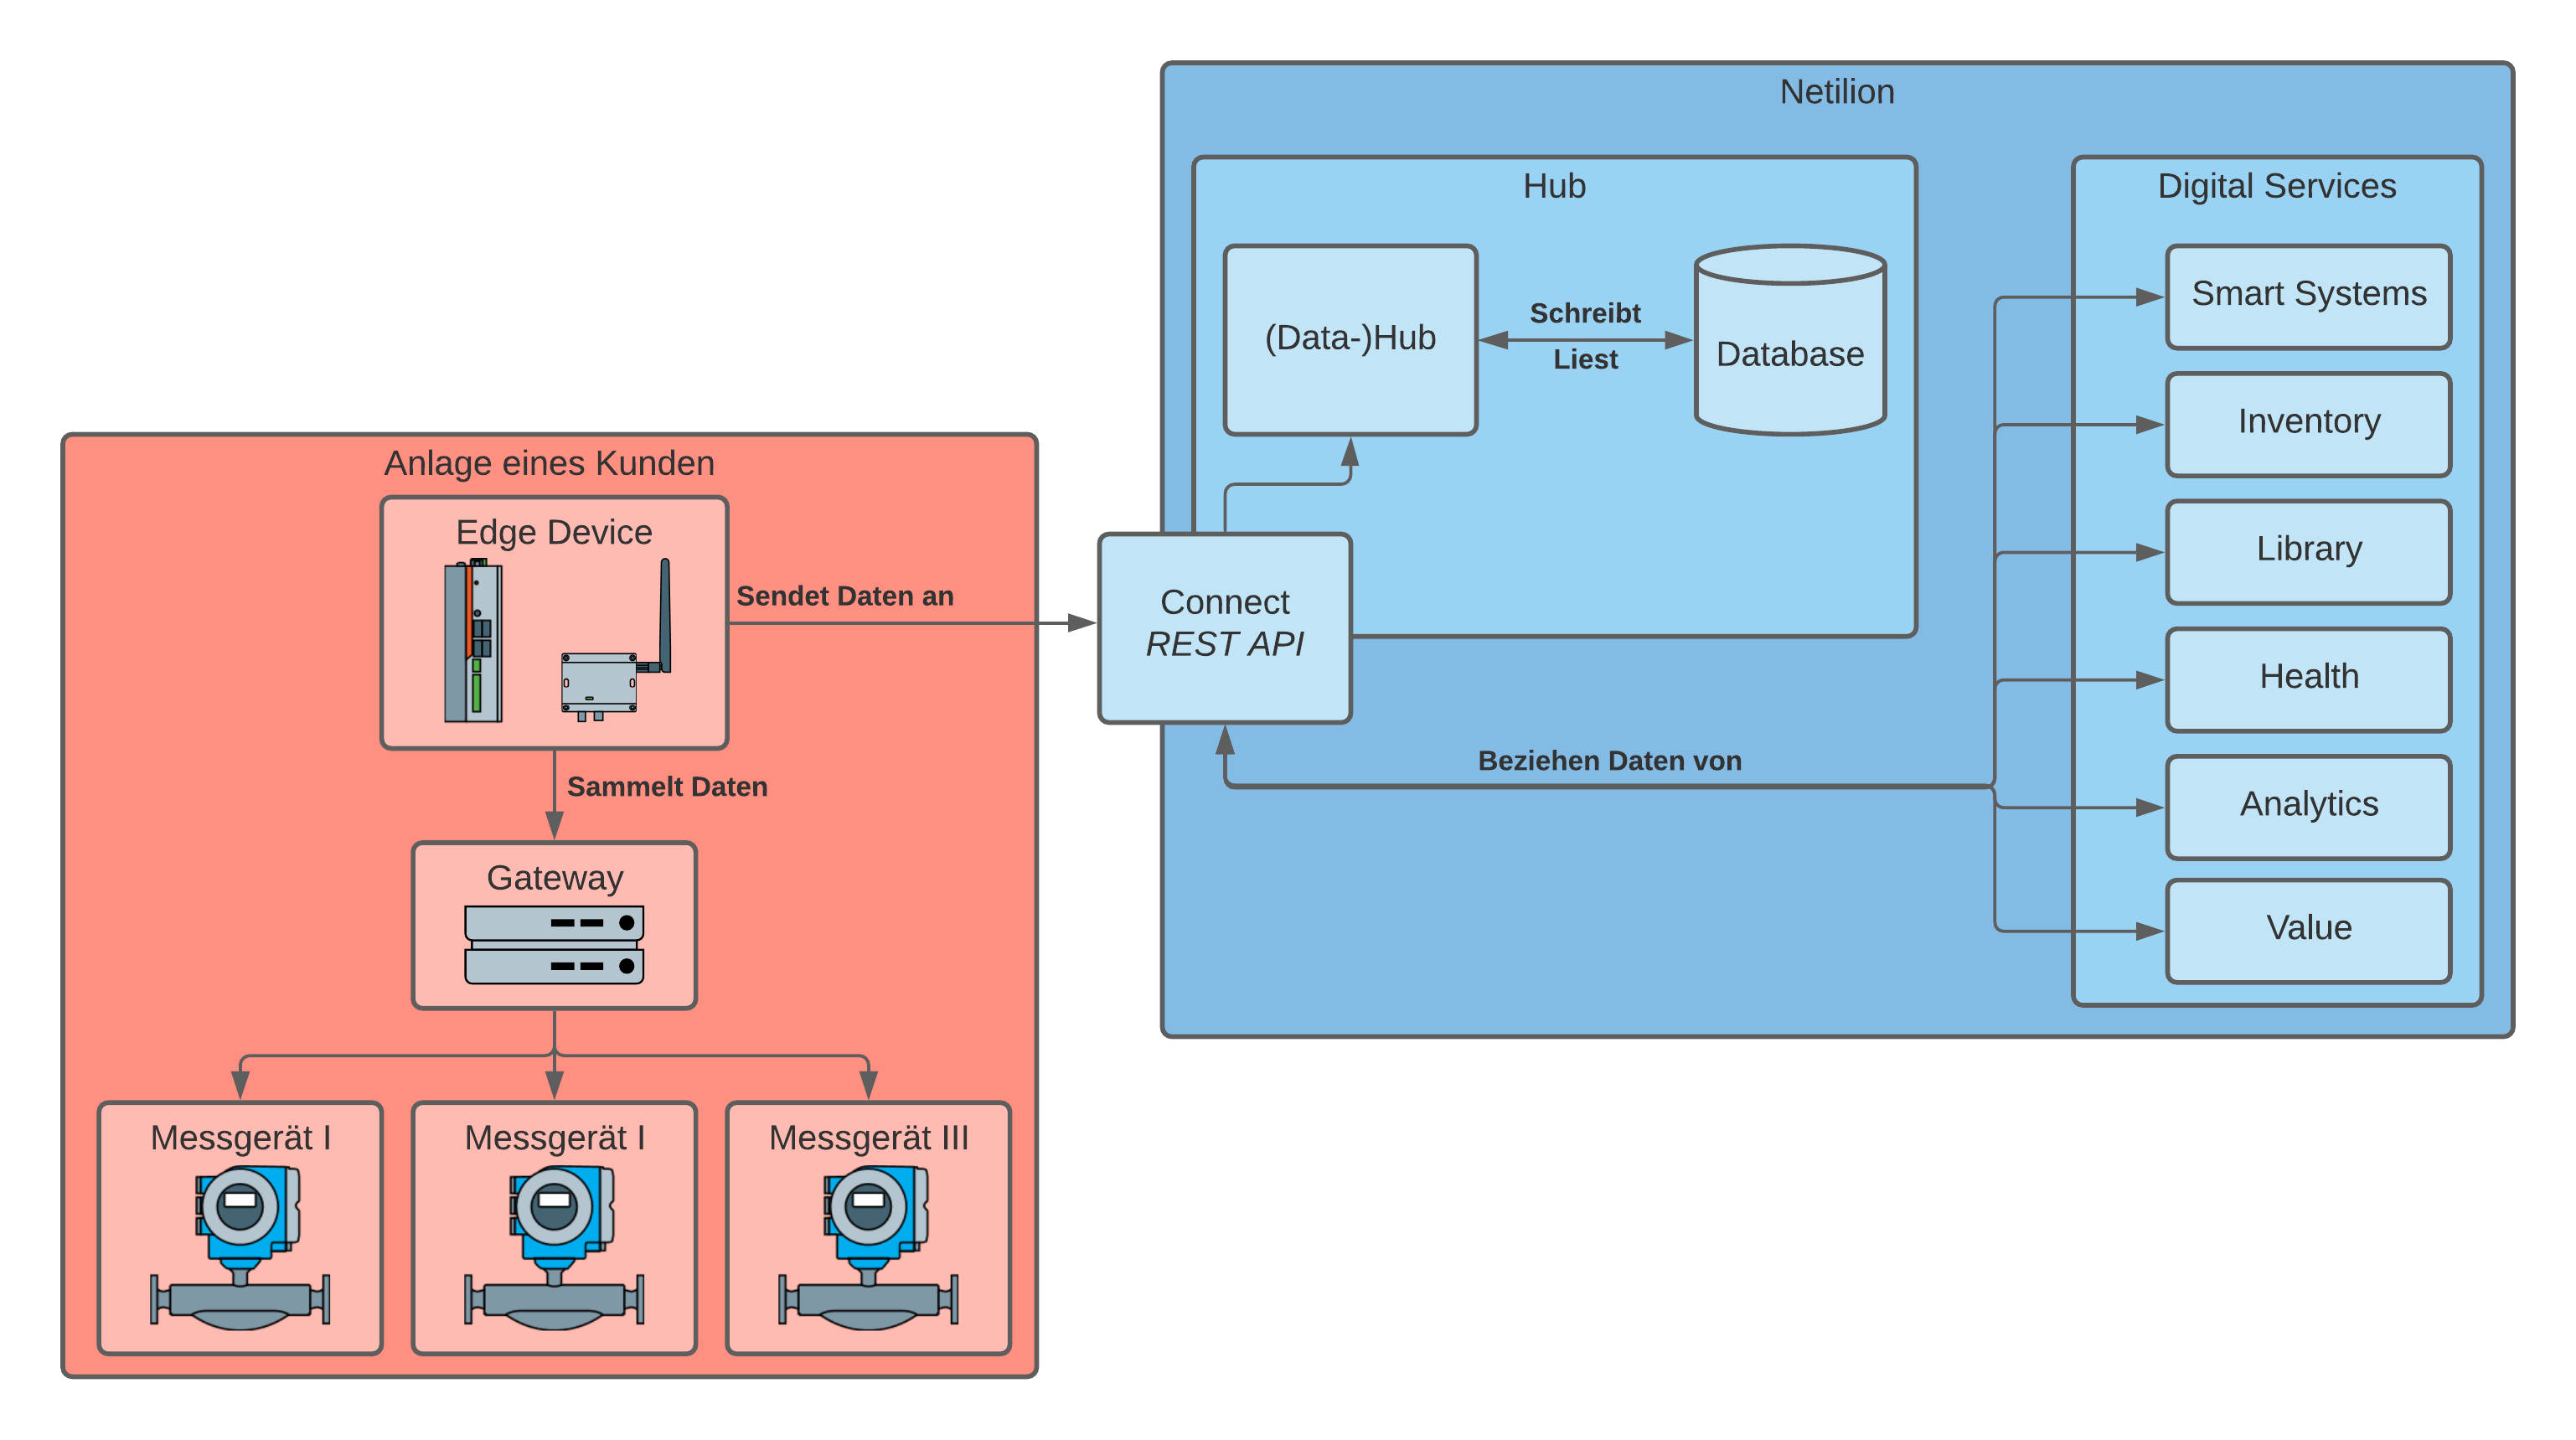
\includegraphics[width=.95\linewidth]{./images/Netilion.png}
  \caption[{Diagramm Netilion Ökosystem von Jonas Schultheiss}]{Netilion Ökosystem}
  \label{fig:netilion}
\end{figure}
Netilion ist das IIoT Ökosystem welches vor einigen Jahren von der Endress+Hauser Digital Solutions ins Leben gerufen wurde. Zuvor hatten Kunden keinen direkten Einblick in die Daten der Messgeräte. Techniker mussten regelmässig vorbei kommen und die Geräte prüfen, auch wenn diese funktionierten. Wenn die Anlage des Kunden an das Internet angebunden ist, erschlissen sich neue Informationsmöglichkeiten über die eingebauten Messgeräte. Genau das ist der Punkt, an dem Netilion mit seinen digitalen Services für den Kunden Mehrwerte liefert.
\newline
Die Daten der Messgeräte werden mithilfe eines Edge Devices ausgelesen und zuerst lokal gespeichert, bevor sie dann in regelmässigen Intervallen an die REST-API von Netilion gesendet werden. Dort werden sie vom Hub empfangen, validiert und serialisiert. Anschliessend kann der Kunde eine der digitalen Services nutzen und die verarbeiteten Daten grafisch aufbereitet ansehen.
\subsubsection{Hub}
Der Hub ist das zentrale Lager aller Daten, welche im Ökosystem verwendet werden. Er bietet die REST-API an, validiert Daten, regelt das Benutzer- und Zugriffssystem und speichert alles in einer Datenbank.
\subsubsection{Digitalen Services}
Die Digitalen Services sind Webapplikationen, welche die Daten der Anlage entgegennehmen, aufbereiten und mit anderen Daten integrieren. So zeigt zum Beispiel die Applikation \amk{Health} die NE107 Status der einzelnen Geräte an. \amk{Value} hingegen stellt unter anderem die Messwerte der Geräte dar. Daneben gibt es noch weitere Services wie in Abbildung \ref{fig:netilion} genannt.


Ziel ist es mit den digitalen Services den Kunden zu helfen Ihre Anlagenverfügbarkeit zu erhöhen, Prozesse zu verinfachen und damit Kosten zu sparen.
\subsubsection{Connect}
Netilion Connect ist ein neues Angebot des Ökosystems. Grosse Kunden wollen entweder eigene eingekaufte oder von Ihren Entwickler hergestellte Systeme verwenden. Deshalb sollten sie auch ausserhalb unserer Applikation an ihre Daten kommen können. So ergibt sich zum Beispiel die Möglichkeit, ein Dashboard mit den Firmen Guidelines zu erstellen.
\subsection{HERE Developer API}
Als Vorarbeit dieser Arbeit wurde recherchiert, wie die Ortung der Modelle implementiert werden kann. Die erste option war Google Maps. Dies stellte sich allerdings als zu aufwändig heraus. Daher wurde nach alternativen gesucht. Mit der \amk{HERE Developer API} wurde diese schlussendlich gefunden.
\newline
Die Ortungsdaten sollen im Backend mit den Daten der Messgeräte von Netilion integriert.
\subsection{OSE-Dashboard: Backend} \label{arch-backend}
\begin{figure}[H]
  \centering
  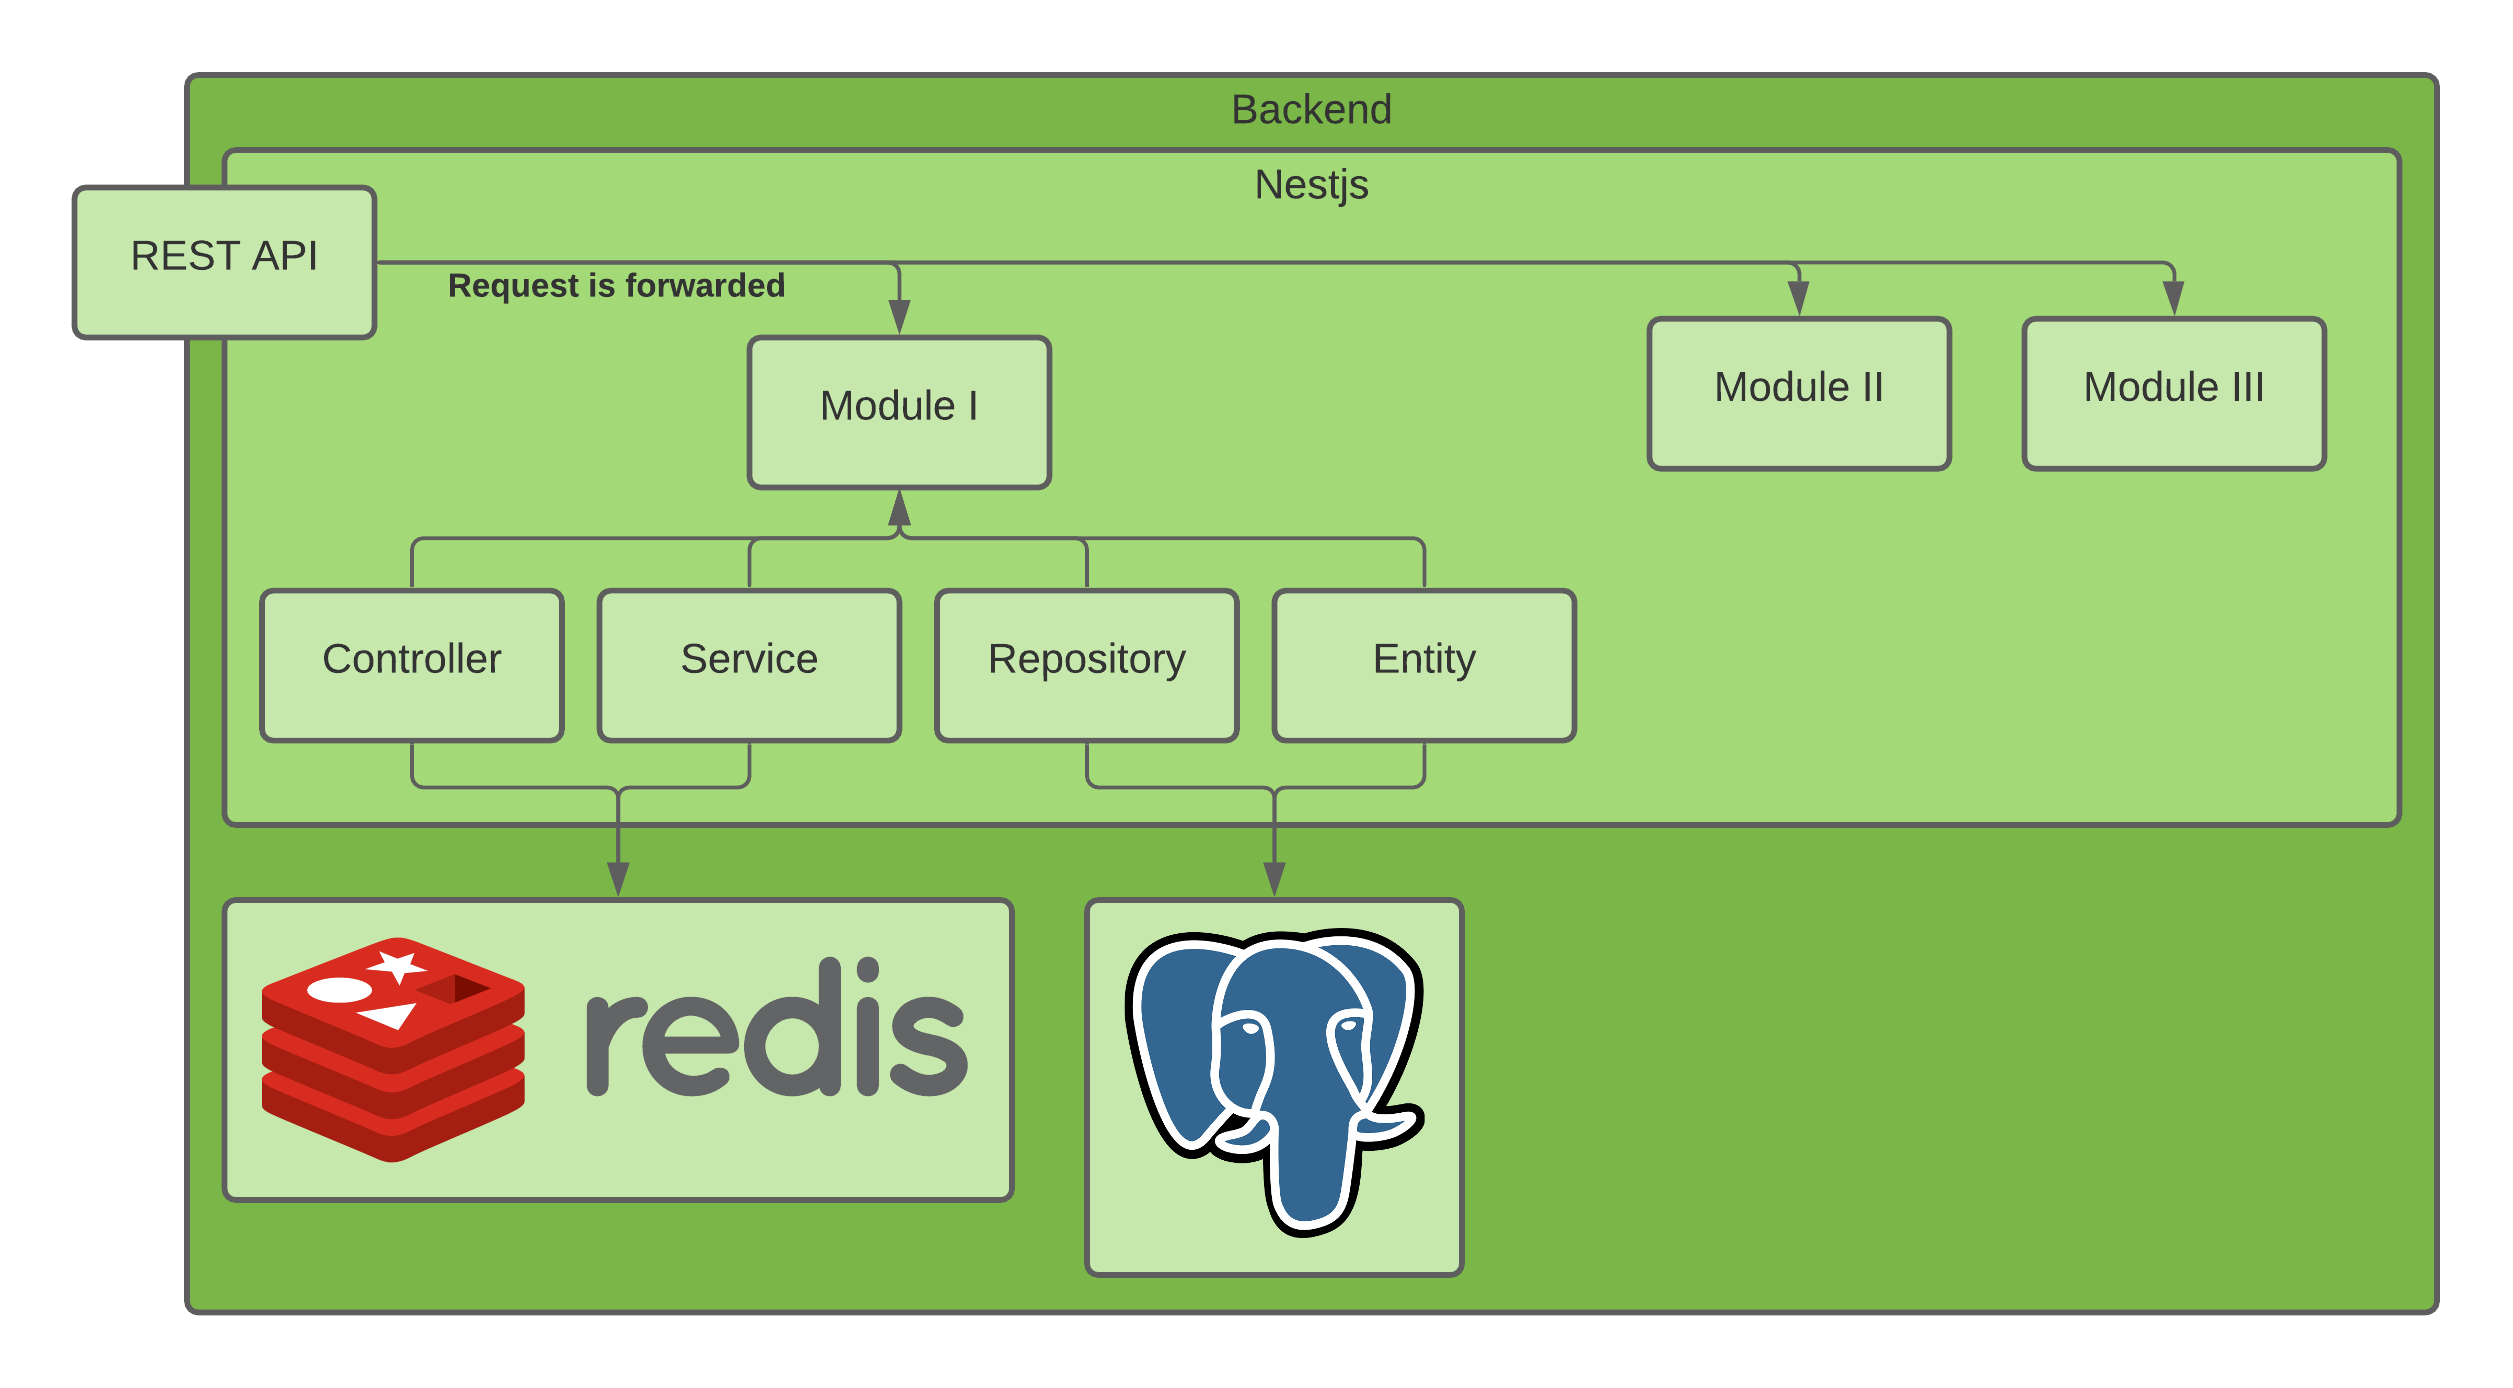
\includegraphics[width=.95\linewidth]{./images/backend.png}
  \caption[{Diagramm OSE-Dashboard Backend von Jonas Schultheiss}]{OSE-Dashboard Backend}
  \label{fig:backend}
\end{figure}
Die Aufgabe des Backends war primär das Cachen der Daten. Ohne Caching würde jede Instanz des Frontends direkt Anfragen an Netilion gesendet. Auch wenn ein Client nur alle 30 Minuten die Daten aktualisiert, wir wissen trotzdem nicht, auf wie vielen Clients unser Frontend gerade aktiv ist. Das Abonnement der REST-API besitzt eine maximale Zahl an Anfragen, welche gemacht werden können, bevor auf die nächste teurere Stufe aufgerüstet werden muss. Diese Nummer nicht zu über- schreiten war ein Kriterium des Product-Owners. Da dies schwierig abzuschätzen oder auszurechnen ist mit einer unbekannten Zahl, wurde das Backend erstellt.


Ein eigenes Backend zu erstellen hat den Vorteil, dass wir zusätzliche Daten anfordern können und diese direkt mit den Netilion-Daten verlinken/integrieren können.


Kurz vor der IPA hat das Team, welches hinter der Entwicklung von Netilion steht, angekündigt, dass Webhooks nun in der Produktion verfügbar sind. Mithilfe von Webhooks kann ein Client einzelne Events abonnieren und erhält direkt Bescheid, wenn sich ein Wert ändert. Mit diesen Webhooks müsste ich keine Intervalle/Cron-Jobs verwenden müssen, wodurch die Anzahl der Anfragen deutlich vermindert werden würde.
\newline
Auch wenn ein Lösungsansatz mit Webhooks optimaler wäre, habe ich mich dagegen entschieden, es an dieser IPA so zu lösen. Das Feature wurde kurz vor der IPA angekündigt und ich habe bisher keine theoretische oder praktische Erfahrung mit Webhooks. Gerne werde ich es nach dem Abschluss der IPA angehen.
\subsubsection{Nestjs}
Seit dem zweiten Lehrjahr arbeite ich mit Javascript. Die Sprache hat mich von Anfang an angesprochen. Der Hauptgrund war, dass man mit Javascript nicht nur ein Frontend erstellen kann, sondern mittlerweile dank Node.js auch Backends/Servers und sogar Apps fürs Smartphone. Wenn ein Produkt im ganzen Stack Javascript verwendet, müssen Entwickler nicht mehrere Sprachen lernen, sondern können sich ganz auf eine Fokussieren, Stücke vom Quellcode können ausgetauscht werden und so weiter.
\newline
Ich habe Erfahrungen mit praktisch allen populären Node.js-Backendframeworks, konnte mich allerdings nie ganz mit einem anfreunden. Die meisten Frameworks sind unopinionated. Dies gefällt mir im Backend nicht, da nach einer kurzen Zeit ein Durcheinander entsteht, welches man dann selber aufräumen kann. Sobald man einen passenden Platz für alles gefunden hat, kann man das gleiche nochmals beim nächsten Projekt wiederholen.
\newline
NestJS geht komplett in eine andere Richtung. Es ist sehr inspiriert von Java Spring und Angular, ist extrem opinionated und das meiste kommt out of the box, ohne das man selber viele Konfigurationen machen muss.
\subsubsection{Inspiration}
Wie in Java Spring Boot gibt es Controller, Services, Repositories und Entitäten. Diese werden jeweils nur für eine Ressource erstellt. Mögliche Ressourcen sind zum Beispiel \amk{Users} oder \amk{Assets}. Wie in Angular werden sie zu einem Modul gebündelt.
\subsubsection{Komponenten einer Nestjs Applikation}
Nestjs ist highly opinionated. Dabei ist vordefiniert, wie der Code struckturiert ist. Entwickler sollten folgendem Schema folgen:
\begin{table}[H]
  \begin{tabularx}{\textwidth}{l X }
  \textbf{Komponente} & \textbf{Beschreibung} \\ \\\hline \\
  Entity & Enthält die Entität, welche vom ORM verwendet wird und als Basisklasse dient\\
  Repository & Erledigt alle direkten Interaktionen mit den Entitäten \\
  Service & Handhabt die Geschäftslogik \\
  Controller & Dient dazu, Anfragen entgegenzunehmen, validieren und den verantwortlichen Service aufzurufen \\
  Module & Bündelt die Komponenten einer Funktion oder Resource, reguliert Imports von anderen Services und Exports von eigenen Services \\
  \\\hline
  \end{tabularx}
\end{table}
\subsubsection{Redis \& Postgresql}
Ich habe mich bei temporärem Caching für Redis entschieden, da ich keine Alternative dazu kenne und da es auch sonst intern verwendet wird. PostgreSQL habe ich genommen, da Netilion und das dahinterstehende Team dies nutzt
\subsubsection{Hosting}
Das Backend wird auf Heroku gehostet. Gründe dafür sind folgende:
\begin{itemize}
  \item Praktische Erfahrung seit dem zweiten Lehrjahr.
  \item Wird intern und bei Netilion verwendet.
  \item Bietet gratis Redis \& PostgreSQL Instanz an, welche für diesen Use-Case komplett ausreichen.
\end{itemize}
\subsection{OSE-Dashboard: Frontend} \label{arch-frontend}
\begin{figure}[!ht]
  \centering
  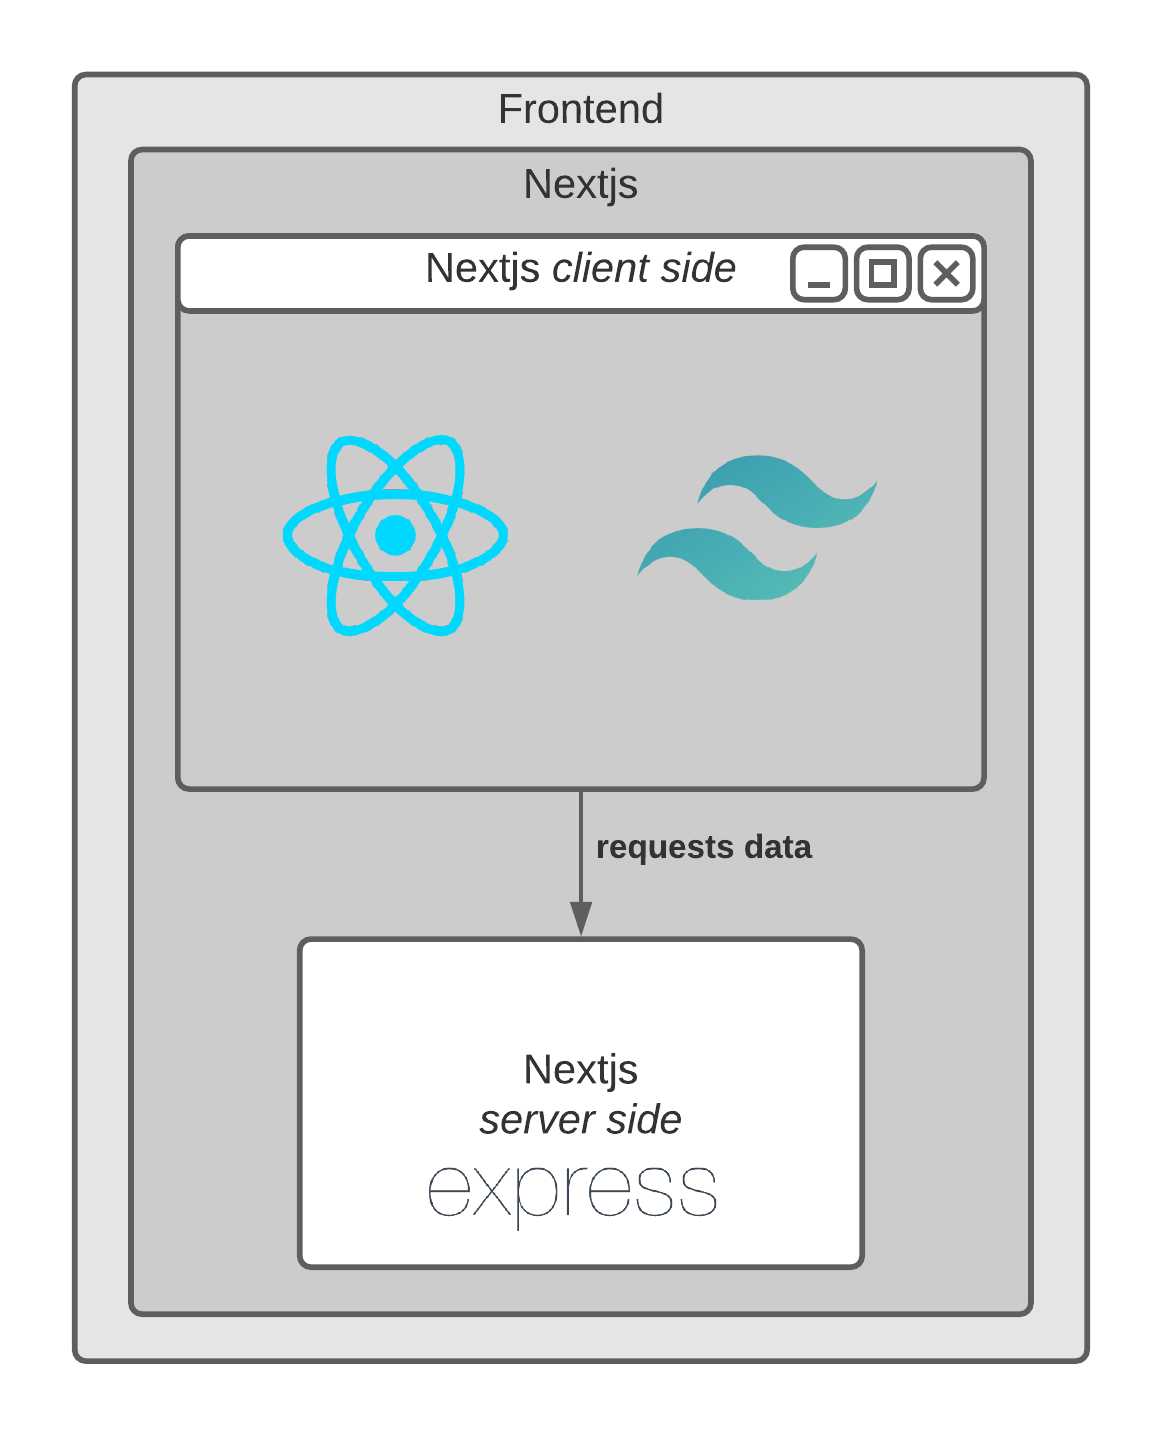
\includegraphics[width=.4\linewidth]{./images/frontend.png}
  \caption[{Diagramm OSE-Dashboard Frontend von Jonas Schultheiss}]{OSE-Dashboard Frontend}
  \label{fig:frontend}
\end{figure}
\subsubsection{Hosting}
Das Hosting wird mit Vercel gemacht. Vercel ist eine amerikanische Firma, die sich auf den JAM-Stack fokussiert. Seit 2016 bietet sie eine sehr vereinfachte Möglichkeit, moderne Javascript Frontends zu builden und deployen. Zeitgleich arbeiten sie auch an Next.js, welches kurze Zeit später veröffentlicht wurde. Next.js ist ein Frontend Framework, welches Routing, Server-side-rendering und viele weitere Features mit React verbindet. Next.js ist für das Hosting auf Vercel optimiert. So ist das Deployment noch einfacher als bei vergleichbaren Frameworks, und es können tiefere Analysewerte gemessen werden.
\subsubsection{Server-side-rendering}
Eines der Features, welches Next.js ausmacht, ist das Server-side-rendering, welches es out of the box anbietet. Dadurch kann man beim Entwickeln angeben, welche Seiten statisch und welche dynamisch sein sollen. So wird nicht nur die Erfahrung des Users besser, man steigert auch das SEO Ranking. Das Framework baut auf express auf. Dies ermöglicht es einem, ein minimales backend in das Frontend einzubauen. Die Vorteile davon sind, dass sensible Daten so nicht beim Benutzer landen.
\section{Ist/Soll-Vergleich}
Ein meiner Meinung nach wichtiger Teil der IPA ist der Vergleich zwischen dem momentan vorhandenen Stand und wie das fertige Produkt aussehen sollte. In den folgenden Kapiteln \ref{ist-zustand} und \ref{soll-zustand} gehe ich auf diese beiden Themen ein.
\subsection{Ist Zustand} \label{ist-zustand}
\subsubsection{Modell}
Bei der Erstellung der Vorarbeit war die Verwendung von mehreren Modellen nie ein Thema. Es sollte extra für Reinach angefertigt werden. Zu diesem Zeitpunkt wusste ich nicht einmal, dass die Endress+Hauser Gruppe noch mehr von ihnen besass, geschweige den, dass sie intern standardisiert wurde. Das heisst, dass immer die gleichen Messgeräte auf den Modellen sind.
\newline
Da es sich nur um ein einziges Modell handelte, habe ich die IDs der digitalen Zwillinge der Messgeräte per Hand herausgesucht und dann statisch in den Quellcode geschrieben. Dies war der einfachste Weg, um das Projekt wie gewünscht umzusetzen. Es gab mir zu diesem Zeitpunkt auch keinen Sinn, das Ganze dynamisch zu gestalten.
\subsubsection{Credentials}
Damit ich die Daten der Messgeräte erhalten konnte, musste ich geheime Zugangsdaten verwenden. Dies wurde von Anfang mit Environmentvariablen gelöst, da ich leider in der Vergangenheit schon einmal erfahren musste, was es heisst, die geheimen Zugangsdaten auf GitHub zu pushen. Anfangs wurde dies mit BasicAuth im Server-Side Teil von Nextjs erledigt. Später habe ich es dann allerdings ins Backend verschoben. Momentan verwendet das Projekt noch diesen statischen Lösungsweg mit BasicAuth.
\subsubsection{Konfiguration}
Da es sich nur um ein Modell handelte, habe ich gewünschte Konfigurationen entweder in Environmentvariablen gespeichert oder direkt in den Sourcecode geschrieben. Da es nun mehrere Modelle sind, muss ein Konfigurationsmenü her.
\subsection{Soll Zustand} \label{soll-zustand}
\subsubsection{Modelle}
Es sollen nun mehrere Modelle eingebunden werden können und ein User soll zwischen den Standorten wechseln können. Dafür müssen neue Entitäten im Backend und neue Tabellen in der Datenbank angelegt werden. Einerseits soll eine \flqq models\frqq Tabelle her, welche die \flqq assets\frqq , also Messgeräte, bündelt. Andererseits muss auch der Standort des Modells abrufbar sein können, weswegen auch eine \flqq locations\frqq Tabelle erstellt werden sollte.
\subsubsection{OAuth2}
In dieser Erweiterung ist es notwendig, dass sich mehrere Netilion-Accounts sicher anmelden können. Ich habe mich in der Vergangenheit sehr intensiv mit OAuth2 beschäftigt und finde, dass ich es optimal für diesen Use-Case umsetzten kann. Sprechen wir allerdings über die Entscheidung, wieso OAuth2 verwendet werden sollte und nicht einfach das bestehende BasicAuth Konstrukt erweitert werden sollte.
\begin{itemize}
  \item BasicAuth wird in der nahen Zukunft nicht mehr unterstützt
  \item OAuth2 verbessert wie User Experience, da ein Nutzer nurnoch seinen Log-in braucht
  \item OAuth2 vermindert den administrativen Aufwand
  \item Die Lösung ist optimaler und schöner
\end{itemize}
\subsubsection{Konfigurationsmenü}
Damit der Verantwortliche eines OSE-Modells Einstellungen vornehmen kann, muss ein Konfigurationsmenü her. Ein Teil der IPA ist es, die digitalen Zwillinge automatisch mit den Meshes des 3D-Modells zu verlinken. Sollte dies aus irgendeinem Grund nicht möglich sein, soll der User dies selbst manuell verlinken können. Damit diese wichtige Einstellung aber nicht von jedem User vorgenommen werden kann, darf nur dies nur ein eingeloggter User, welcher sich in einer Usergroup befindet, vornehmen.
\section{Namenskonzept}
\subsection{User-Stories}
\begin{table}[H]
  \begin{tabularx}{\textwidth}{l l X}\hline \\
  \textbf{Segment} & \textbf{Abkürzung} & \textbf{Beschreibung} \\ \\\hline \\
  1 & US & Abkürzung für User-Story \\
  2 & - & Trennzeichen \\
  3 & 01 & Fortlaufende Kennzahl \\
  \\\hline
  \end{tabularx}
\end{table}
\subsection{Akzeptanzkriterien}
\begin{table}[H]
  \begin{tabularx}{\textwidth}{l l X}\hline \\
    \textbf{Segment} & \textbf{Abkürzung} & \textbf{Beschreibung} \\ \\\hline \\
    1 & AK & Abkürzung für Akzeptanzkriterium \\
    2 & - & Trennzeichen \\
    3 & 01 & Fortlaufende Kennzahl \\
    \\\hline
  \end{tabularx}
\end{table}
\section{Versionskontrolle}
Ich werde Git mit GitHub verwenden, da ich nun drei Jahre damit gearbeitet habe und mein Lehrbetrieb die gleiche Strategie verfolgt. Dabei werde ich immer nach Abschluss eines Abschnittes einen Commit erstellen. Wichtig ist, dass der Master Branch immer problemlos läuft und deployed werden kann.
\newline
\newline
Diese IPA ist in drei Teile aufgebrochen: das Frontend, das Backend und die Dokumentation. Für alle drei Teile verwende ich Git \& GitHub. Hier ist eine auflistung aller Repositories:
\begin{table}[htp]
  \begin{tabularx}{\textwidth}{l X}
  Frontend: & \href{https://github.com/EndressHauser-ProcessSolutions/ose-dashboard-frntnd}{EndressHauser-ProcessSolutions/ose-dashboard-frntnd} \\
  Backend: & \href{https://github.com/EndressHauser-ProcessSolutions/ose-dashboard-bcknd}{EndressHauser-ProcessSolutions/ose-dashboard-bcknd} \\
  Dokumentation & \href{https://github.com/EndressHauser-ProcessSolutions/ose-dashboard-docs}{EndressHauser-ProcessSolutions/ose-dashboard-docs} \\
  \end{tabularx}
\end{table}
\subsection{Git Flow}
\begin{figure}[!ht]
  \centering
  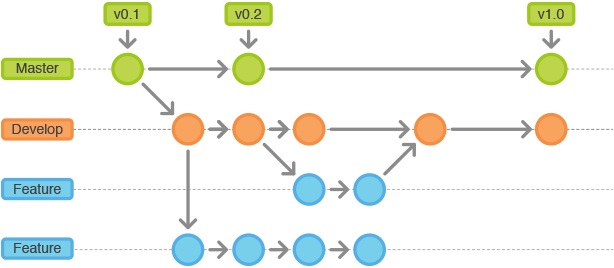
\includegraphics[width=0.8\linewidth]{./images/Gitflow-Workflow-2.png}
  \caption[\href{https://blog.ordix.de/welches-vorgehen-eignet-sich-fuer-mein-projekt}{Grafik, welche den Git Flow Arbeitsablauf visualisiert}]{Git Flow visualisiert}
  \label{fig:git-flow}
\end{figure}
Mit dem Git Flow definiert ein Team oder ein Entwickler, wie sie/er die Versionskontrolle in Git handhabt. Es gibt drei Arten von Branches:
\begin{itemize}
  \item \textbf{Master} - Enthält immer die lauffähige und stabile Version, welche gerade deployed ist.
  \item \textbf{Develop} - Dies ist der Branch, auf dem entwickelt wird. Er soll immer lauffähig sein, damit neue Features getestet werden können, bevor er mit dem Master zusammengeführt wird.
  \item \textbf{Feature} - Die Einzelnen Stories und Tasks werden in einem Feature Branch entwickelt. Sobald das Feature fertig ist, kann es in den Develop Branch gemerged werden.
\end{itemize}
Diese Strategie bietet einige Vorteile:
\begin{itemize}
  \item Der Master Branch kann mithilfe von CI/CD automatisch deployed werden. So erreichen neue Features schneller den Kunden
  \item Der Develop Branch kann auch mit CI/CD automatisch deployed werden, damit Features intern einfacher und schneller besprochen werden können.
  \item Durch die klare Abtrennung dieser Branches erhöht sich die Stabilität der Software, was die Kundenzufriedenheit erhöht.
  \item Features können abgekapselt entwickelt werden.
  \begin{itemize}
    \item Develop Branch bleibt dadurch immer lauffähig
    \item Mehrere Features können gleichzeitig entwickelt werden, ohne sich in die Quere zu kommen
    \item Bietet bessere Übersicht auf GitHub
  \end{itemize}
\end{itemize}
\subsection{Pipelines zu Vercel und Heroku}
Vercel und Heroku bieten Build-Pipelines an. Mit diesen kann ein Branch mit Vercel oder Heroku verbunden werden. Wird ein neuer Commit gepusht, triggert dies den Buildprozess von Vercel oder Heroku, woraufhin man kurze Zeit später eine live Version hat.
\newline
\newline
Ich werde jeweils zwei Pipelines einrichten. Einmal die Produktionsumgebung mit dem Master Branch und einmal die Testumgebung mit dem Develop Branch.
\subsection{Dokumentation}
Die Dokumentation ist in LaTeX geschrieben und wird regelmässig auf GitHub in ein separates Repository gepusht. Im GitHub habe ich ausserdem ein GitHub Action eingerichtet, welche nach jedem push getriggert wird, das Dokument als PDF rendert und zum Download zur Verfügung stellt.
\newline
\newline
Bei der Versionierung dieses Dokumentes orientiere ich mich an meiner Einschätzung verbunden mit folgendem System:
\begin{table}[htp]
  \begin{tabularx}{\textwidth}{l l X}\hline \\
  \textbf{Versionsartefakt} & \textbf{Beispiel} & \textbf{Beschreibung} \\ \\\hline \\
  1 & 0 & \textbf{Major} Grosse Abschlüsse des Dokumentes \\
  2 & . & Trennzeichen \\
  3 & 1 & \textbf{Minor} Eine Änderung wie z.B. ein neues Kapitel \\
  4 & . & Trennzeichen \\
  5 & 3 & \textbf{Patch} Kleine Änderung / Neue Texte in einem Kapitel \\
  \\\hline
  \end{tabularx}
\end{table}
\newline
Wichtig zu beachten ist, dass ich bei der Dokumentation \textbf{nicht GitFlow einsetzte}, da es keinen Vorteil für den Aufwand bietet.
\section{Backupkonzept}
Die ganze Dokumentation und jeglicher Code wird mindestens einmal täglich auf GitHub gepusht. Optimal ist, wenn der Code im Falle vom Front- und Backend nach jedem Feature gepusht wird und bei der Dokumentation nach der fertigstellung eines Unterkapitels. Sollte was verloren gehen kann man so also immer mindestens auf den letzten Stand des Vorabends zurückzuspringen.
\newline
\newline
Das MacBook wird mithilfe vom vorinstallierten Tool \flqq Time Machine\frqq ständig inkrementell auf einer externen SSD gesichert. Time Machine speichert dabei Folgendes \cite{apple_2021_mit}:
\begin{itemize}
  \item Lokale Schnappschüsse, solange Speicherplatz vorhanden ist
  \item Stündliche Backups der letzten 24 Stunden
  \item Tägliche Backups des letzten Monats
  \item Wöchentliche Backups aller vorherigen Monate
\end{itemize}
Somit ist eine schnelle Weiterarbeit trotz Hardwareproblemen möglich.
\subsection{Sicherheit der Daten}
Die Repositories befinden sich auf dem GitHub Team der Firma. Dieses Team ist so sicher eingerichtet, wie es GitHub erlaubt. Meine Accounts verwenden beide sichere Passwörter und Two-Way-Authentificator.
\newline
Die interne SSD des MacBooks \cite{a2021_hardware} und die externe SSD \cite{a2021_keep} sind verschlüsselt.
\section{Personas}
\begin{figure}[!ht]
  \centering
  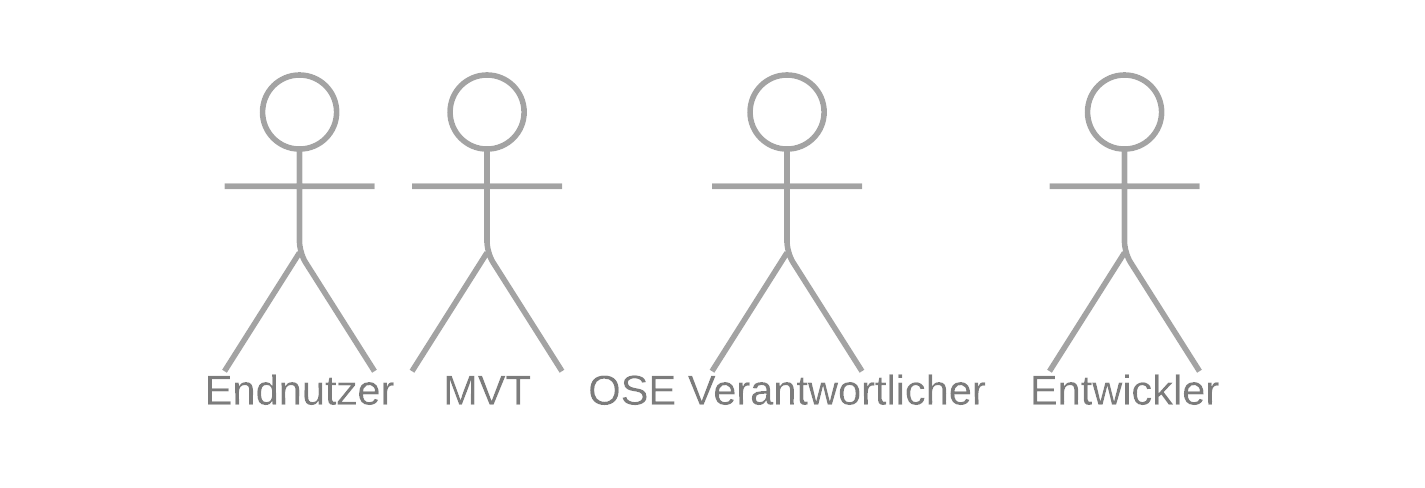
\includegraphics[width=0.6\linewidth]{./images/Personas.png}
  \caption[Personas]{Personas}
  \label{fig:personas}
\end{figure}
\subsection{Endnutzer}
Der Endnutzer ist schlussendlich der Besucher, welcher am Fernseher mit dem Dashboard interagiert. Er möchte möglich einfach die Daten des OSE-Modells ansehen können, ohne sich dabei einloggen zu müssen.
\subsection{MVT}
Das MVT Team ist für interne und externe Trainings unseres Portfolios zuständig. Markus Reisgis von MVT war der originale Auftraggeber. Für sie ist wichtig, dass alle gewünschten Daten korrekt angezeigt werden und das der Endnutzer eine gute Erfahrung macht.
\subsection{OSE Verantwortlicher}
Der OSE Verantwortliche ist die Person, welche für ein Modell verantwortlich ist. Dies ist zum Beispiel MVT in Reinach. Es gibt einige Weitere in Deutschland, Frankreich und so weiter. Für sie ist wichtig, dass sie wenig Mehraufwand haben. Im optimalen Fall sollte Log-in und die eventuelle Konfiguration möglichts einfach und fehlerfrei ablaufen.
\subsection{Entwickler}
Der Entwickler bin ich. Mir ist es wichtig, alle gewünschten Features kompetent und wie gewünscht umzusetzen, und dabei den Fortschritt korrekt zu dokumentieren.
\section{User Stories}
\subsection{US-01}
Als OSE Verantwortlicher möchte ich mich einloggen können, damit ich mein Modell registrieren kann.
\begin{itemize}
  \item AK-01 Log-in möglich
  \item AK-02 Log-in Daten sind geschützt und nicht von einem Benutzer auslesbar
  \item AK-03 Bei einem Fehlversuch wird eine passende Fehlermeldung angezeigt
\end{itemize}
\subsection{US-02}
Als OSE Verantwortlicher möchte ich, dass die digitalen Zwillinge der Messgeräte automatisch verlinkt werden, ohne das ich etwas machen muss, solange sie standardisiert sind.
\begin{itemize}
  \item AK-01 Automatische Verlinkung bei Registrierung funktioniert, solange die Assets nach dem Standard benannt sind
  \item AK-02 Methode, welche die Verlinkung vornimmt, ist mit automatischen Tests abgedeckt
\end{itemize}
\subsection{US-03}
Als OSE Verantwortlicher möchte ich ein Konfigurationsmenü, mit welchem ich die V§erlinkung manuell ändern kann, sollte ich ein Gerät austauschen.
\begin{itemize}
  \item AK-01 Konfigurationsmenü ist aufrufbar
  \item AK-02 Verlinkungen sind manuell veränderbar
\end{itemize}
\subsection{US-04}
Als OSE Verantwortlicher möchte ich sicher sein, dass kein Endnutzer die Verlinkung ändern kann.
\begin{itemize}
  \item AK-01 Konfigurationsmenü ist nur aufrufbar, solange der OSE Verantwortliche eingeloggt ist
  \item AK-02 Konfigurationsmenü ist nur aufrufbar, solange sich der Account in einer spezifischen User Gruppe befindet
\end{itemize}
\subsection{US-05}
Als Endnutzer möchte ich die Applikation nutzen können, ohne mich einloggen zu müssen.
\begin{itemize}
  \item AK-01 Applikation ist weiterhin ohne Log-in nutzbar
\end{itemize}
\subsection{US-06}
Als Endnutzer möchte ich die Datenquelle des OSE-Dashboards aus den verfügbaren Standorten auswählen können, damit ich auch Daten anderer Modelle sehen kann.
\begin{itemize}
  \item AK-01 Standort kann geändert werden
  \item AK-02 Übersicht über alle verfügbaren Standorte ist implementiert
\end{itemize}
\section{OAuth2 Strategie}\label{oauth2-strat}
\subsection{Was ist OAuth2?}
OAuth2 wurde ins Leben gerufen, um einen spezifischen Use-Case zu decken. Eine Applikation eines Drittanbieters möchte zum Beispiel Daten des Users von Spotify abrufen. Vor OAuth2 musste der User seine Log-in-Daten an den Drittanbieter senden, welcher diese dann in Klartextformat abspeichern musste, damit er später selber die Daten abrufen kann.
\newline
Der User hatte so keine Kontrolle über die Aufbewahrung der Log-in-Daten und wusste schon gar nicht was der Drittanbieter alles mit den Log-in-Daten anstellt. Zusammengefasst war der ganze Prozess sehr unsicher und der User übergab immer alle Rechte des Accounts.
\newline
\newline
Mit OAuth2 konnte dieser Prozess nun sicher gestaltet werden. Der User wird auf die Anmeldeseite des OAuth2-Providers weitergeleitet und meldet sich dort an. So kommt die Applikation des Drittanbieters zu keinem Zeitpunkt an die Log-in-Daten. Als nächstes wird dem User gezeigt, auf was für Daten der Drittanbieter zugriff haben möchte. Akzeptiert der User, wird er wieder zurück an den Drittanbieter weitergeleitet, welcher mit diesem Schritt einen Zugriffstoken erhält. Dieser ist nur von dieser Applikation und auf diesen User nutzbar, um die Daten, die der User freigegeben hat, anzufragen.
\pagebreak
\subsection{Anwendung im OSE-Dashboard}
\begin{figure}[!ht]
  \centering
  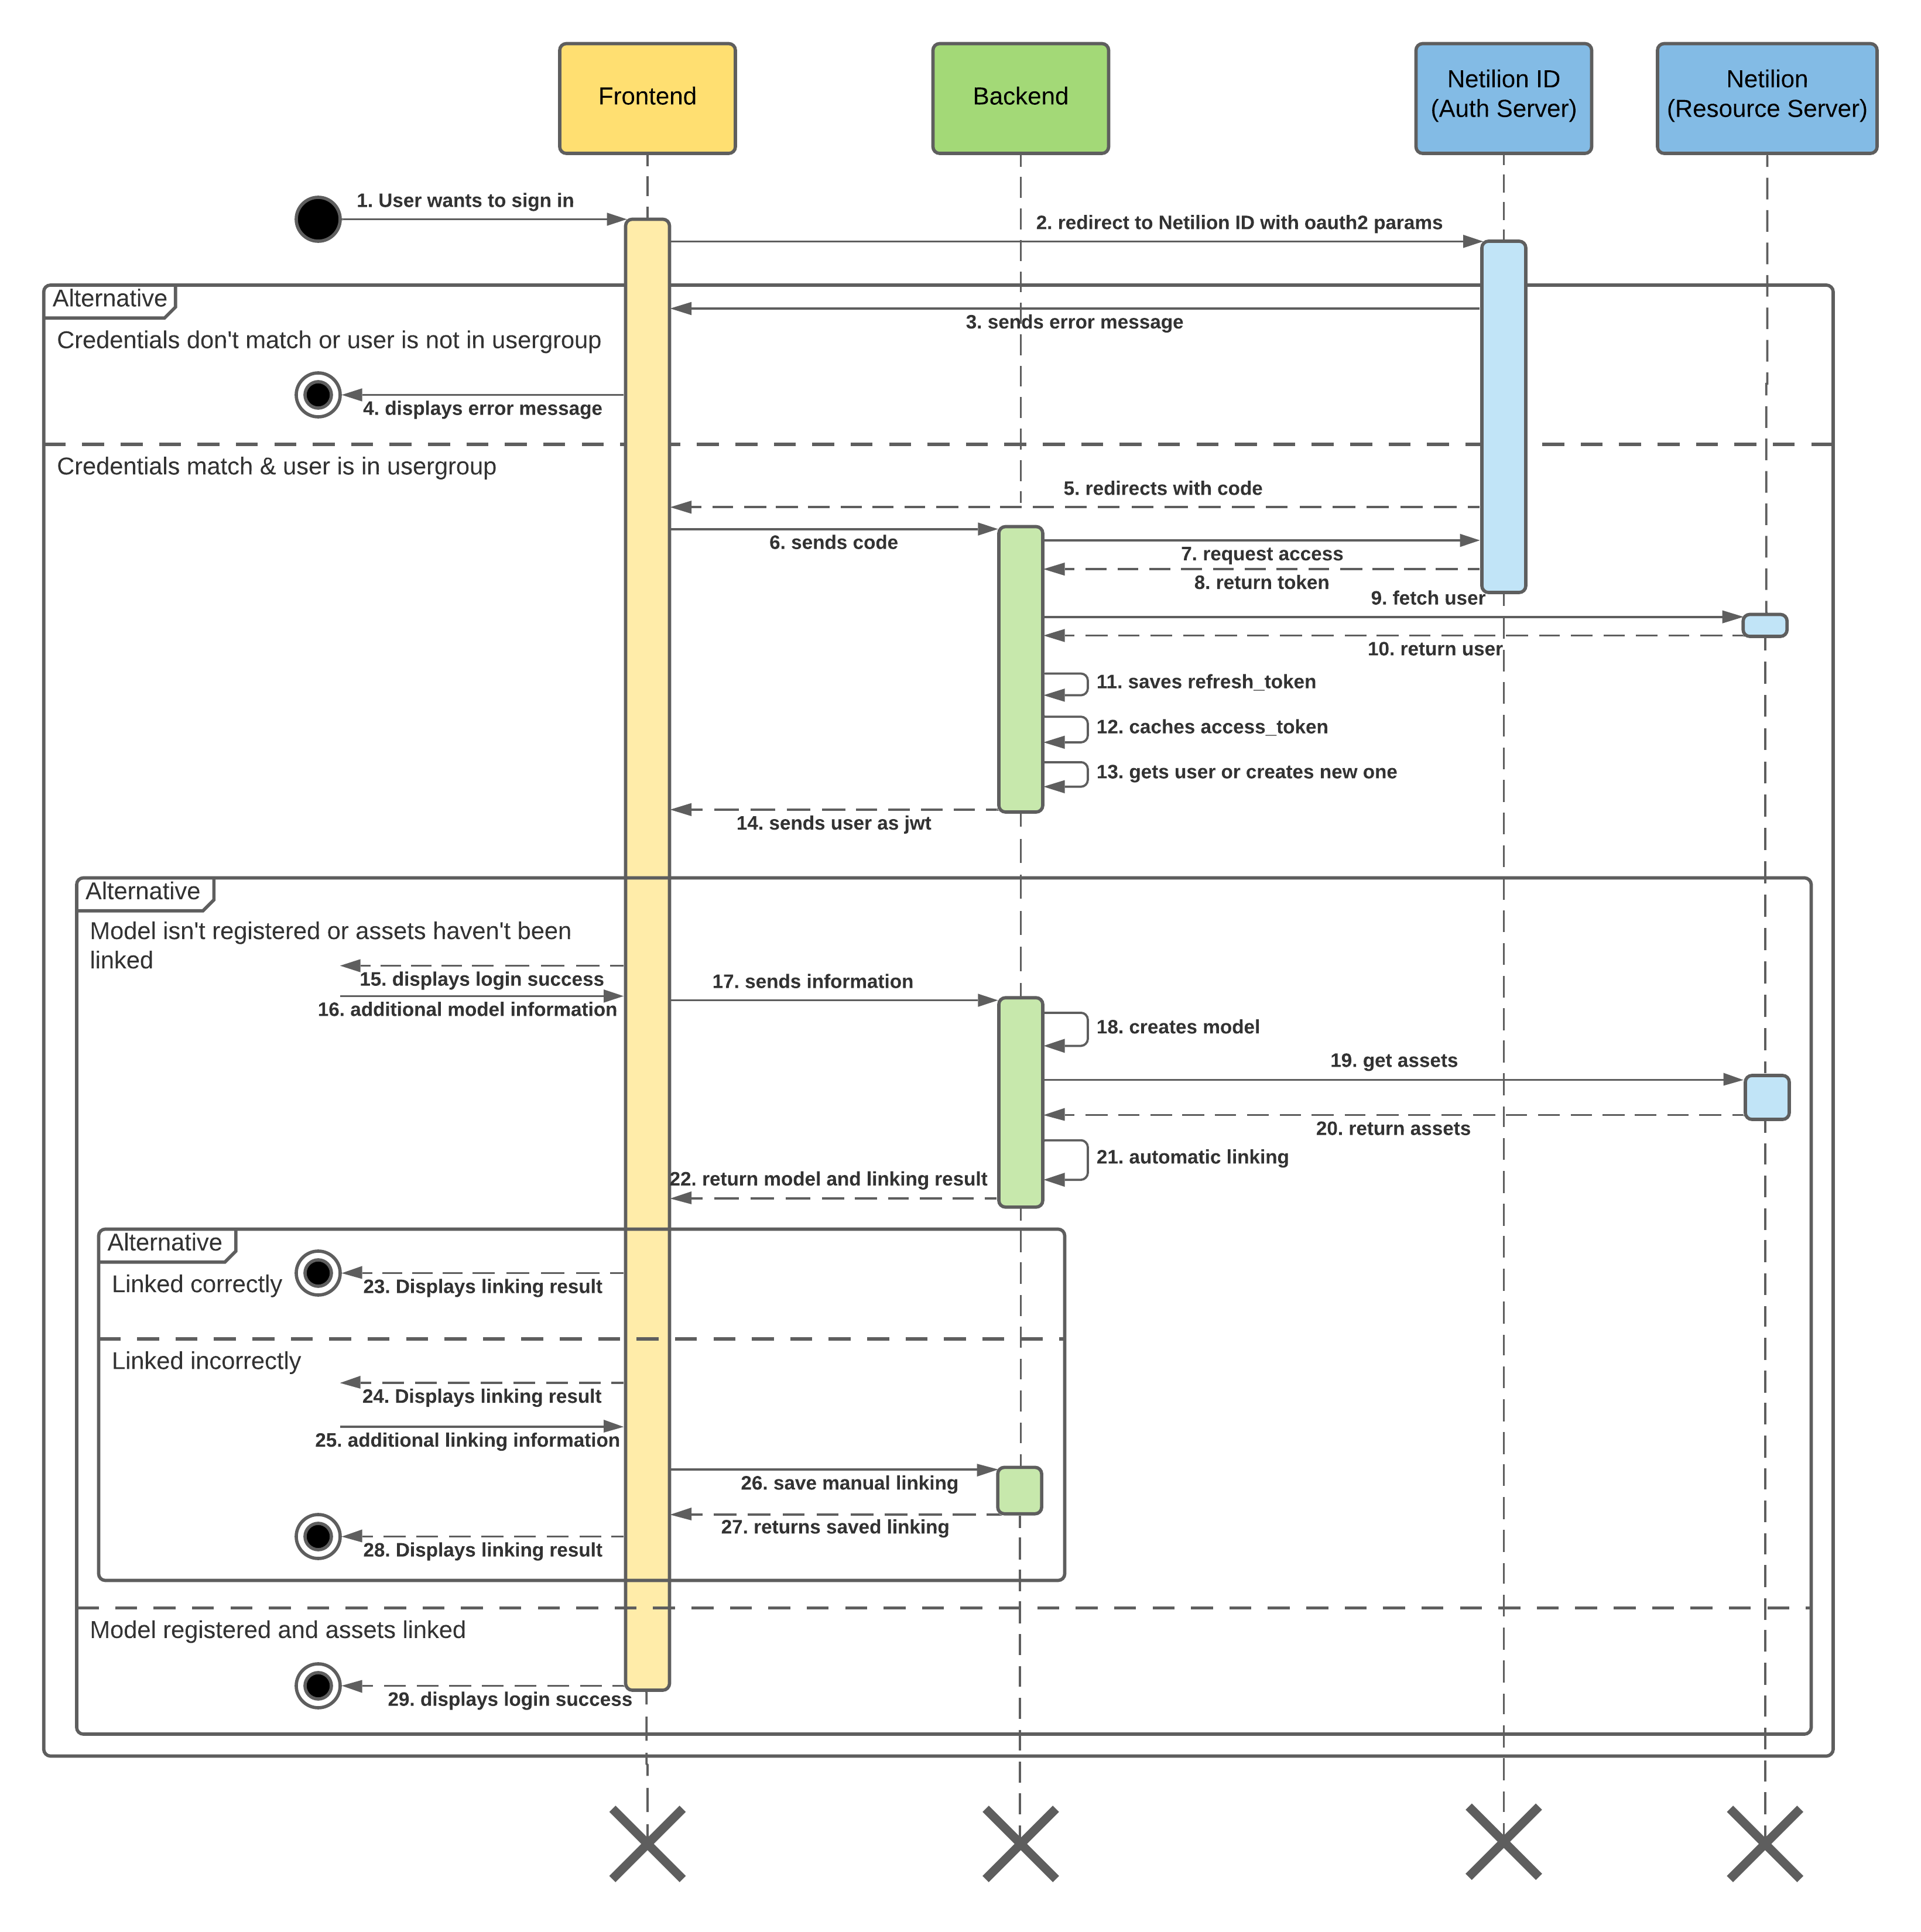
\includegraphics[width=1\linewidth]{./images/OAuth2.png}
  \caption[OAuth2 visualisiert durch ein Sequenzdiagramm]{OAuth2 visualisiert durch ein Sequenzdiagramm}
  \label{fig:oauth2}
\end{figure}
Folgend ist eine Auflistung der einzelnen Schritte, welche in der Abbildung \ref{fig:oauth2} dargestellt sind.
\begin{enumerate}
  \item Der User will sich einloggen und klickt auf ein \code{<a></a>} tag.
  \item Daraufhin wird er zu Netilion ID weitergeleitet. Die URL enthält dabei die \code{client\_id} und \newline\code{redirect\_uri}. Dadurch weiss Netilion, welche Applikation die Anfrage macht und wohin der User nach der Anmeldung weitergeleitet werden möchte.
  \item Gibt es ein Problem mit dem Log-in, erhält die \code{redirect uri}, also das Frontend, eine Fehlermeldung.
  \item Das Frontend nimmt die Fehlermeldung entgegen und stellt sie für den User dar.
  \item Wenn alles korrekt ablauft, wird der Client mit einem code wieder an unser Frontend weitergeleitet.
  \item Dieser Code wird direkt an das Backend gesendet.
  \item Mit diesem Code kann das Backend dann einen Zugriffstoken anfordern.
  \item Dieser wird von Netilion ID an unser Backend geschickt.
  \item Mit diesem Zugriffstoken ist es dann möglich, Daten von Netilion abzufragen, in diesem Fall der User.
  \item Die Daten des Users werden anschliessend zurückgeschickt.
  \item Der \code{refresh\_token} wird verschlüsselt und in der Datenbank gespeichert.
  \item Der \code{access\_token} wird in redis gecached.
  \item Existiert der User, wird dieser aus der Datenbank gelesen. Existiert er nicht, wird ein neuer erstellt.
  \item Der User wird als JWT zurück ans Frontend geschickt.
  \item Das Frontend zeigt an, dass die Anmeldung erfolgreich verlief.
  \item Wenn das Modell noch nicht registriert wurde oder die Messgeräte noch nicht verlinkt wurden, wird der User nach zusätzlichen Daten wie dem Standort gefragt.
  \item Das Frontend schickt diese Daten mit dem JWT an das Backend.
  \item Das Backend erstellt ein neues Modell mit den Daten des Users.
  \item Anschliessend fragt es bei Netilion nach allen Messgeräten nach.
  \item Netilion antwortet mit allen Messgeräten des Users.
  \item Daraufhin erfolgt die automatische Verlinkung.
  \item Das Modell mitsamt verlinkten Messgeräten wird ans Frontend weitergeleitet.
  \item Stimmt die Verlinkung ist der Nutzer zufrieden und der Prozess beendet.
  \item Stimmt die Verlinkung nicht, da der Nutzer nicht die standardisierten Geräte oder benennungen verwendet, wird ihm das Resultat angezeigt.
  \item Daraufhin verlinkt der User selbst die Geräte.
  \item Dies wird ans Backend gesendet, damit die Änderungen gespeichert werden können.
  \item Die gespeicherten Änderungen werden an das Frontend geschickt.
  \item Der User wird benachrichtigt, dass seine Änderungen übernommen wurden. Der User ist zufrieden und der Prozess beendet.
  \item Ist das Modell bereits registriert und die Messgeräte verlinkt, ist der Prozess beendet.
\end{enumerate}


\chapter{Entwurf}
\section{Generelles Abfragen von Daten} \label{data-fetching}
Dieses Abschnitt baut auf das Kapitel \ref{oauth2-strat} auf.
\begin{figure}[!ht]
  \centering
  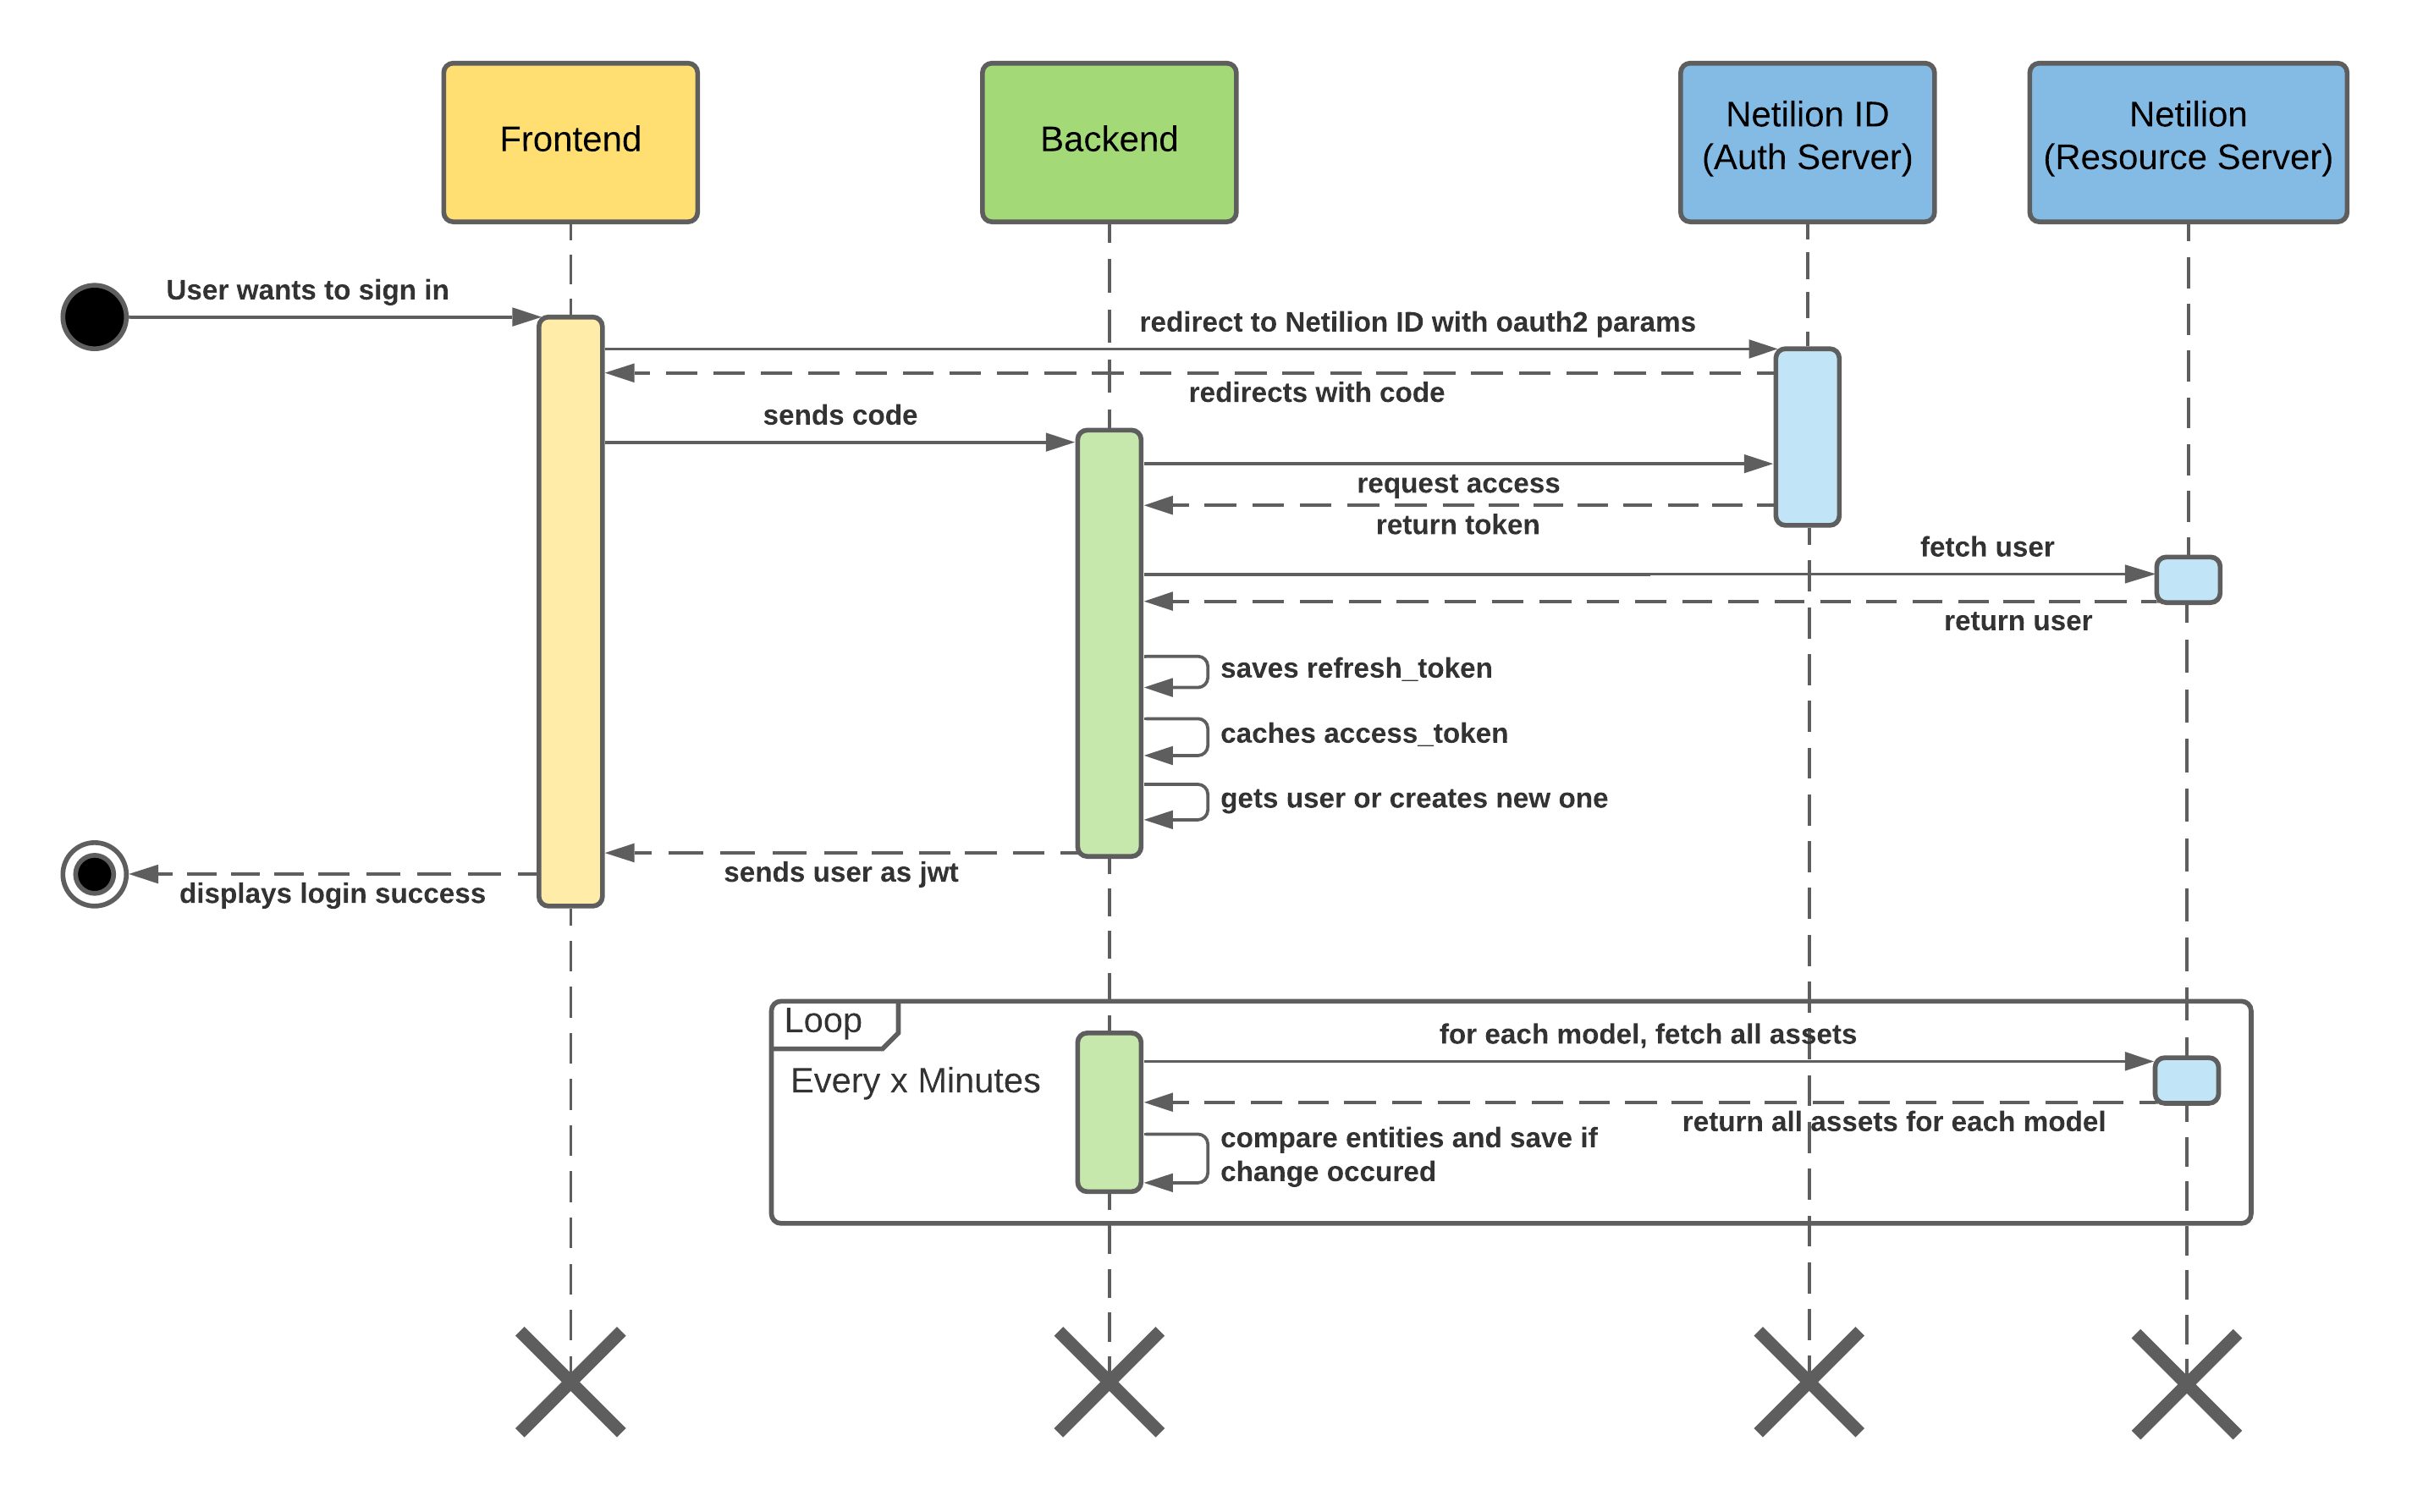
\includegraphics[width=.95\linewidth]{./images/datafetching.png}
  \caption[{Sequenzdiagram, welches das automatische fetching Erklärt}]{Data fetching in Intervallen}
  \label{fig:data-fetching}
\end{figure}
Nachdem sich ein OSE Verantwortlicher das erste mal eingeloggt hat, wird der \code{access\_token} in Redis gecached und der \code{refresh\_token} in der Datenbank gespeichert. Die Funktion soll entweder den gecachten Token nehmen und direkt zurückgeben oder mit dem \code{refresh\_token} einen neuen Anfordern, welcher wiederum gecached und zurückgegeben werden soll. Damit ist es dann möglich, dass das Backend selbst die Daten auffrischen kann. Dafür werde ich das Task-Scheduling\cite{a2021_documentation} feature von Nestjs verwenden. Damit ist es möglich eine Funktion wiederholt laufen zu lassen.
\newline
Bevor ich allerdings das ganze automatisieren kann, brauche ich eine Helferfunktion. Denn jede Anfrage an Netilion braucht einen validen \code{access\_token} und er muss auch dem Netilion Benutzer gehören, unter welchem die Messgeräte registriert sind. Mit dieser Function wird es möglich sein das ganze zu vollautomatisieren. Wenn nun ein Benutzer des OSE-Dashboards sich die Daten nun ansehen möchte, kann er dies machen, ohne den Login des jeweiligen OSE Verantwortlichen wissen zu müssen.
\pagebreak
\section{Zugriffskontrolle}
\subsection{OSE Verantwortlicher}
\begin{figure}[H]
  \centering
  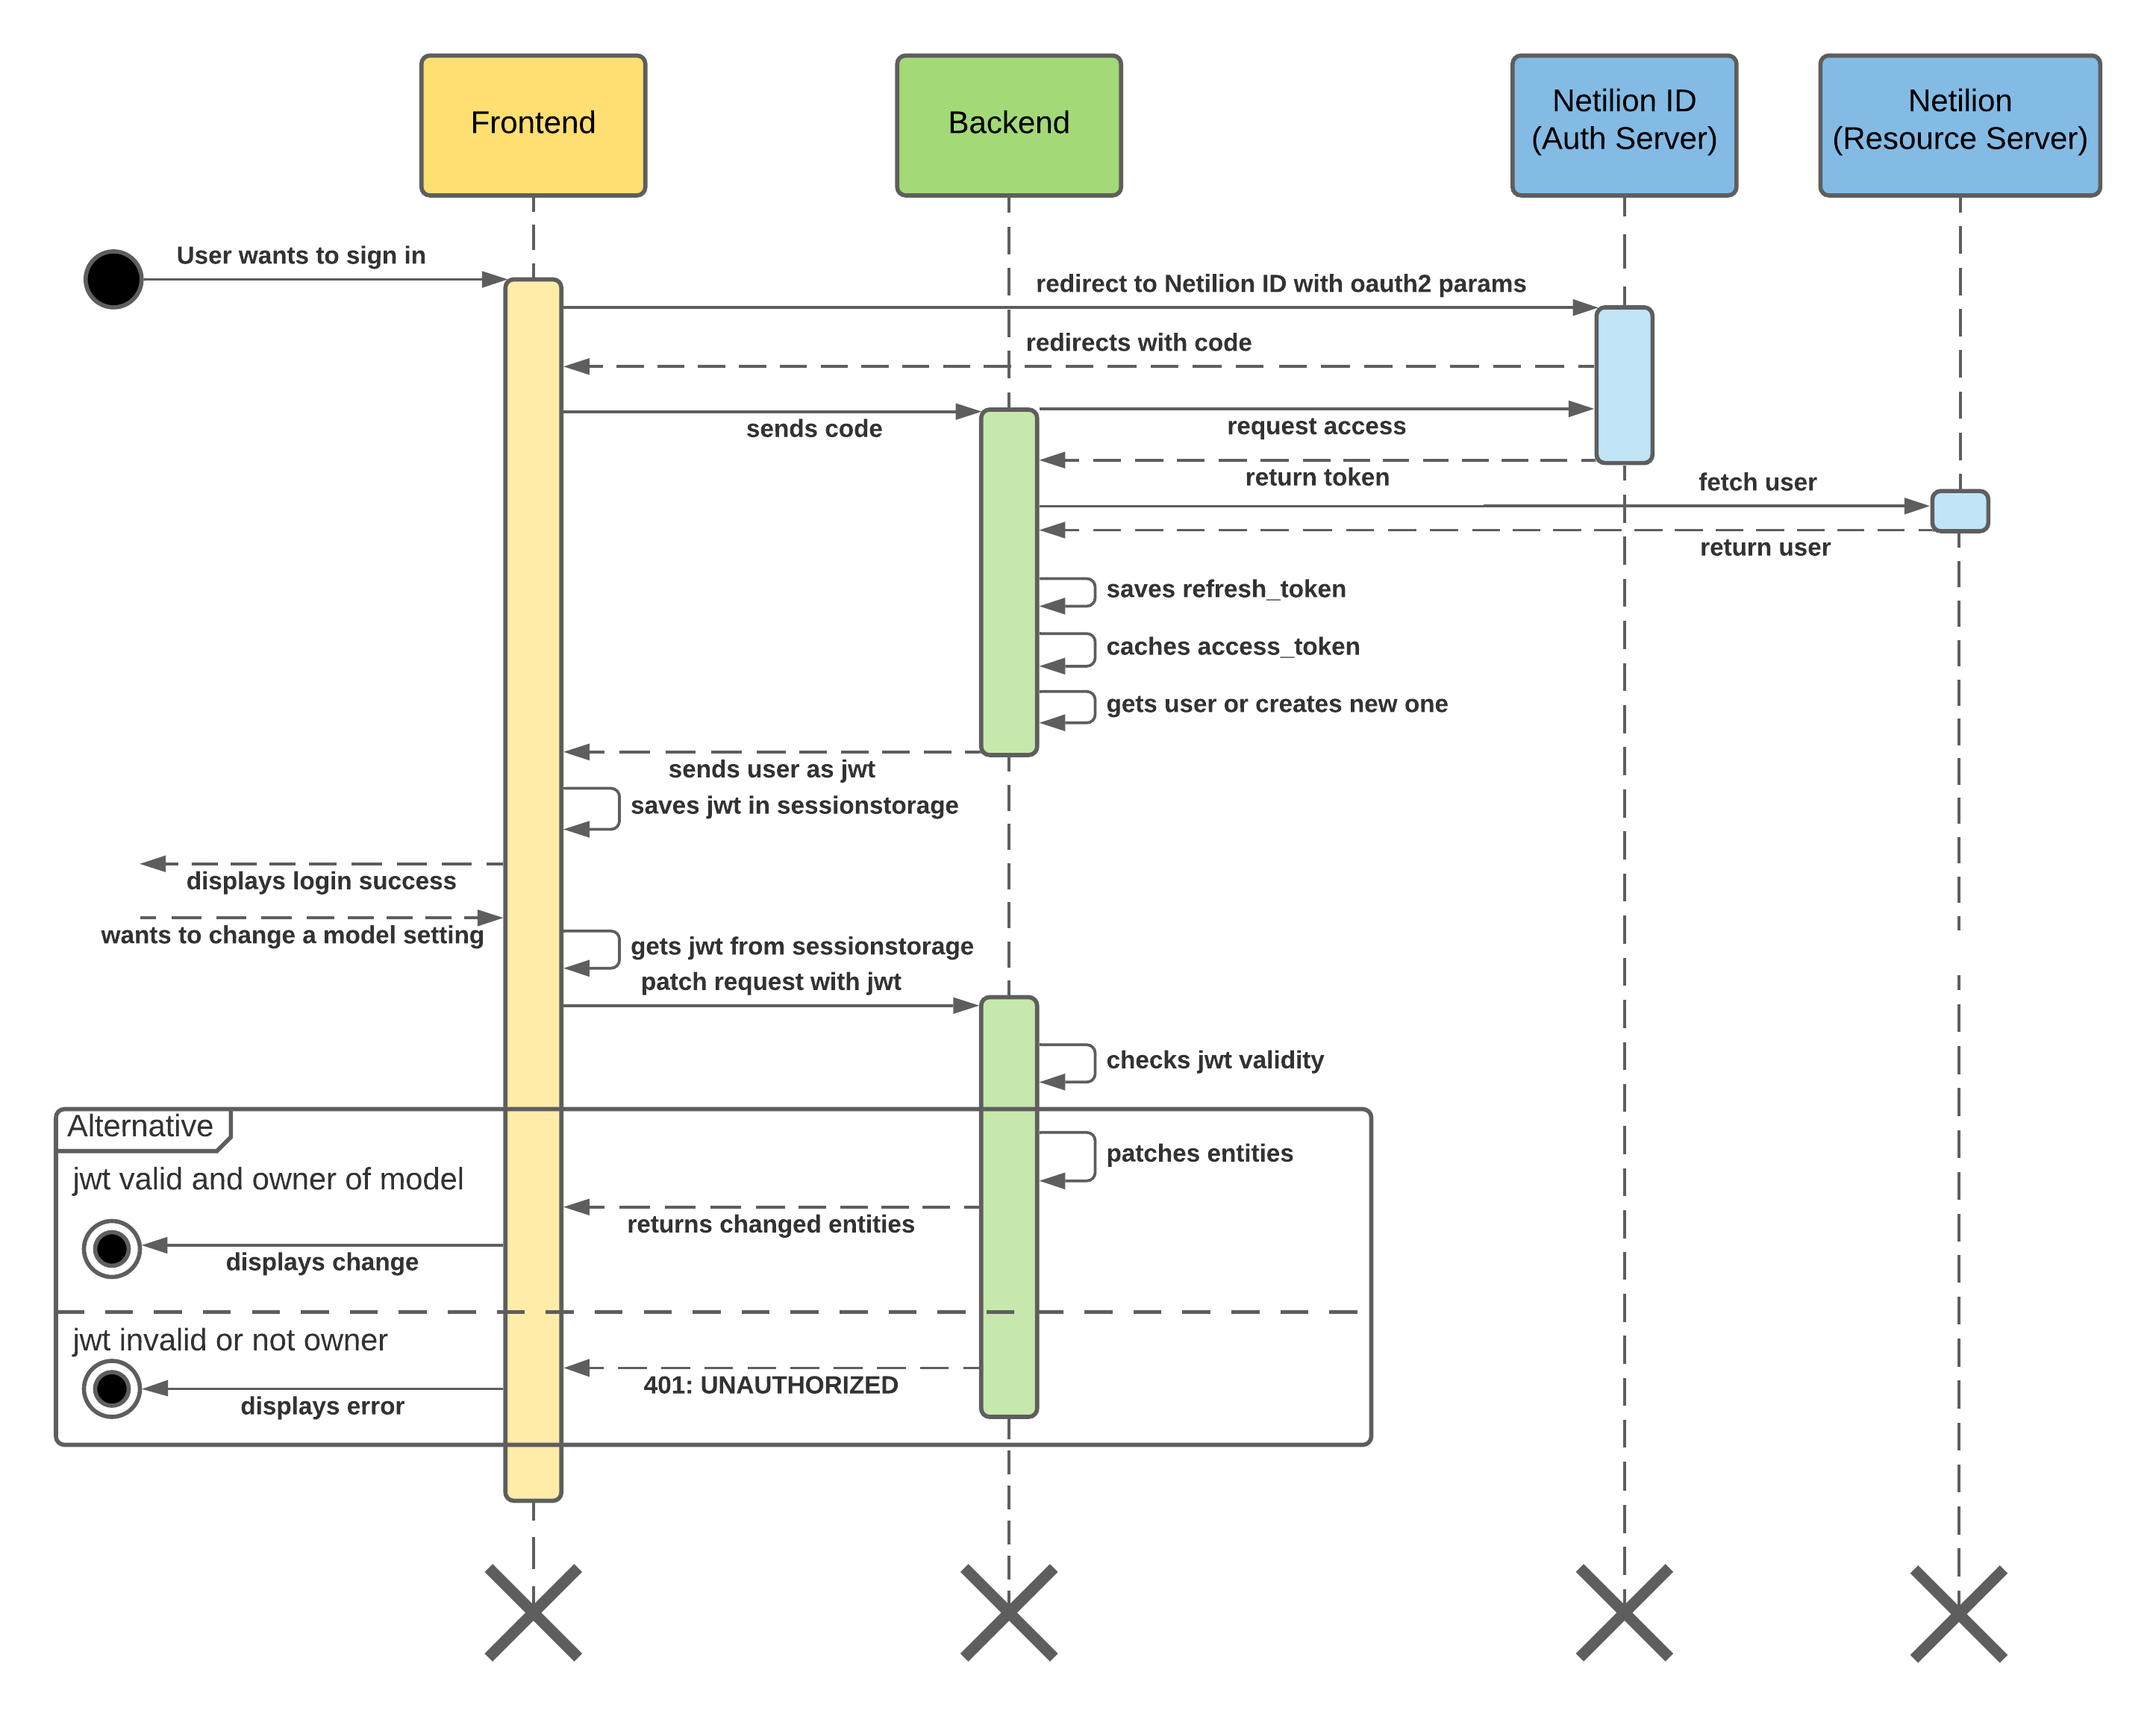
\includegraphics[width=.95\linewidth]{./images/zugriffskontrolle.png}
  \caption[{Sequenzdiagram, welches die Zugriffskontrolle für den OSE Verantwortlichen beschreibt}]{Zugriffskontrolle OSE Verantwortlicher}
  \label{fig:zugriffskontrolle}
\end{figure}
Ein OSE Verantwortlicher soll das Konfigurationsmenü seines Modells öffnen können. Verantwortlicher anderer Modelle oder normale User sollen dies nicht können.
Das ganze sollte folgenderweise gelöst werden:
\newline
Das Frontend erhält nach dem erfolgreichen Login einen JWT. Dieser wird zuerst benötigt, um den Link zum Konfigurationsmenü überhaupt erst im Frontend anzuzeigen. Ausserdem wird er als Authentifizierungsmethode zum Backend verwendet. Der REST Endpoint vom Backend wird durch eine Nestjs Guard\cite{nest_guards} geschützt. Daraufhin wird direkt geprüft werden, ob das Modell auch wirklich dem User gehört. Sollte dies nicht der Fall sein, wird die Anfrage als unauthorized zurückgeschickt.
\subsection{OSE-Dashboard Nutzer}
\begin{figure}[H]
  \centering
  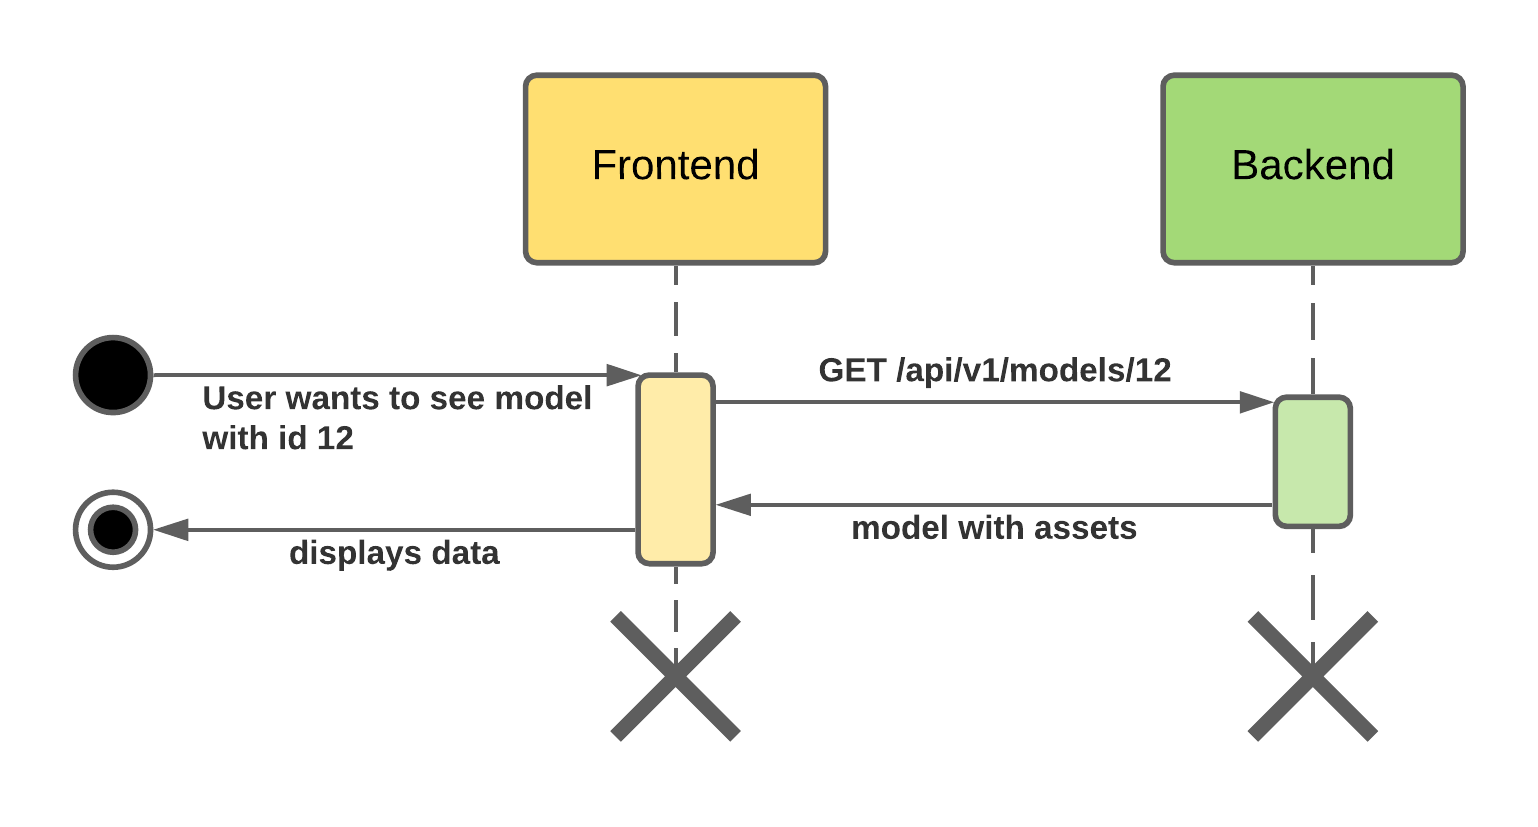
\includegraphics[width=.6\linewidth]{./images/zugriffskontrolle2.png}
  \caption[{Sequenzdiagram, welches die Zugriffskontrolle für den OSE-Dashboard Nutzer beschreibt}]{Zugriffskontrolle OSE-Dashboard Nutzer}
  \label{fig:zugriffskontrolle2}
\end{figure}
Der OSE-Dashboard möchte sich alle OSE-Modelle ansehen können, ohne sich dabei einloggen zu müssen.
Das ganze sollte folgenderweise gelöst werden:
\newline
Wie in Kapitel \ref{data-fetching} angesprochen, sind die aktuellen Daten im Backend verfügbar. So ist es also gar nicht nötig Netilion direkt anzufragen. Das Backend soll stattdessen die Daten mit einem public Endpoint verfügbar machen. Auf diesem Weg umgehen wir auch die maximale Anfragen an Netilion, welche in Kapitel \ref{arch-backend} beschrieben wurde.
\newline
So kann das Frontend beliebig oft die Daten abfragen, ohne das sich ein User einloggen muss oder das wir die Grenze der Connect Subscription übertreten.
\section{Softwareschnittstellen}
Die zu erweiterbare Webapplikation ist in mehrere logische Schichten unterteilt. Jede Schicht ist für einen konkreten Teil der kompletten Lösung verandwortlich. Eine vereinfachte Darstellung der Lösung ist bereits in der Abbildung \ref{fig:systemarchitektur} dargestellt. Folgend sind alle Schichten und deren Zuständigkeit zusammengefasst:
\begin{table}[H]
  \begin{tabularx}{\textwidth}{l X}\hline \\
  \textbf{Schicht} & \textbf{Zuständigkeit}  \\ \\\hline \\
  OSE & Daten der Messgeräte in der Anlage werden von einem Edge Device gesammelts und an Netilion gesendet \\
  Netilion & IIoT-Service von Endress+Hauser \\
  Backend & Backend des OSE Dashboards \\
  HERE Developer API & API Eines Drittanbieters. Wird verwendet für das Abfragen von Koordinaten oder Addressen und für die Darstellung der Karte. \\
  Frontend & Frontend des OSE Dashboards \\
  \\\hline
  \end{tabularx}
\end{table}
\subsection{Schnittstellen im OSE}
Wie und welche Daten das OSE Modell an Netilion schickt ist für diese Arbeit nicht relevant und wird daher nicht dokumentiert. Allerdings ist es wichtig zu wissen, dass die Daten gesammelt und in Intervallen an Netilion gesendet werden.
\subsection{Netilion}
Folgend sind die verwendeten Schnittstellen von Netilion aufgelisted. Von den angeforderten Entitäten werden nur die verwendeten Attribute vermerkt und beschrieben. Um zusätzliche Informationen über die Entitäten zu erhalten, sollten die offizielle \href{https://api.iiot.endress.com/doc/v1/}{Netilion API Dokumentation} aufgesucht werden.
\subsubsection{API Routes}
\begin{table}[H]
  \begin{tabularx}{\textwidth}{l X X}\hline \\
  \textbf{Anfrage} & \textbf{Pfad} & \textbf{Antwort}  \\ \\\hline \\
  HTTP:GET & \code{/users/current} & NetilionUser \\
  HTTP:GET & \code{/assets} & Array of Asset \\
  \\\hline
  \end{tabularx}
\end{table}
\subsubsection{NetilionUser}
\begin{table}[H]
  \begin{tabularx}{\textwidth}{l l X}\hline \\
  \textbf{Attribut} & \textbf{Datentyp} & \textbf{Beschreibung}  \\ \\\hline \\
  id & number & Primary Key \\
  email & string & Email mit der sich der Nutzer auf Netilion registriert hat \\
  \\\hline
  \end{tabularx}
\end{table}
\subsubsection{Asset}
\begin{table}[H]
  \begin{tabularx}{\textwidth}{l l X}\hline \\
  \textbf{Attribut} & \textbf{Datentyp} & \textbf{Beschreibung}  \\ \\\hline \\
  id & number & Primary Key \\
  serial\_number & string & Seriennummer des Messgerätes \\
  description & string & Beschreibung des Messgerätes \\
  production\_date & string & Produktionsdatum des Messgerätes \\
  last\_seen\_at & string & Wann sich das Messgerät zuletz bei Netilion gemeldet hat \\
  product & number & Foreign Key\\
  status & number & Foreign Key \\
  instrumentations & number & Foreign Key \\
  \\\hline
  \end{tabularx}
\end{table}
\subsubsection{Status}
Der Health-Status des Messgerätes. Zeigt zum Beispiel an, ob das Gerät gewartet werden muss.
\begin{table}[H]
  \begin{tabularx}{\textwidth}{l l X}\hline \\
    \textbf{Attribut} & \textbf{Datentyp} & \textbf{Beschreibung}  \\ \\\hline \\
    id & number & Primary Key \\
    code & string & Standartisierter Status Code \\
    description & string & Beschreibung des Status \\
    name & string & Name des standartisierten Status Codes \\
    \\\hline
  \end{tabularx}
\end{table}
\subsubsection{Instrumentations}
Instrumentations ist der interne Begriff für die Messstelle, an der sich das Messgerät befindet. Wird auch Tag genannt.
\begin{table}[H]
  \begin{tabularx}{\textwidth}{l l X}\hline \\
    \textbf{Attribut} & \textbf{Datentyp} & \textbf{Beschreibung}  \\ \\\hline \\
    id & number & Primary Key \\
    tag & string & Bezeichnung der Messstelle \\
    description & string & Beschreibung der Messstelle \\
    criticality & string & Kritikalität der Messstelle \\
    accessibility & string & Erreichbarkeit der Messstelle \\
    \\\hline
  \end{tabularx}
\end{table}
\subsubsection{Product}
Ein Product ist ein Typ von Messgerät. Product bildet dabei das allgemeine Produkt ab, während dem Asset ein Zwilling eines hergestellten Messgerätes vom Typ Product ist.
\begin{table}[H]
  \begin{tabularx}{\textwidth}{l l X}\hline \\
  \textbf{Attribut} & \textbf{Datentyp} & \textbf{Beschreibung}  \\ \\\hline \\
  id & number & Primary Key \\
  product\_code & string & Code des Produktes \\
  name & string & Name des Produktes \\
  description & string & Beschreibung des Produktes \\
  manufacturer & number & Foreign Key \\
  \\\hline
  \end{tabularx}
\end{table}
\subsubsection{Manufacturer}
Der Manufacturer ist der Hersteller eines Messgerätes.
\begin{table}[H]
  \begin{tabularx}{\textwidth}{l l X}\hline \\
  \textbf{Attribut} & \textbf{Datentyp} & \textbf{Beschreibung}  \\ \\\hline \\
  id & number & Primary Key \\
  name& string & Name des Herstellers \\
  \\\hline
  \end{tabularx}
\end{table}
\pagebreak
\subsection{Backend}
Folgend sind die verwendeten Schnittstellen von \code{ose-dashboard-bcknd} aufgelisted.
\subsubsection{API Routes}
\begin{table}[H]
  \begin{tabularx}{\textwidth}{l X X}\hline \\
  \textbf{Anfrage} & \textbf{Pfad} & \textbf{Antwort}  \\ \\\hline \\
  \textbf{Models} & & \\
  HTTP:POST & \code{/models/:modelId/assets/:assetId} & Void \\
  HTTP:POST & \code{/models/:id/autolink} & Void \\
  HTTP:POST & \code{/register} & Model \\
  HTTP:GET & \code{/models} & Array of Models \\
  HTTP:GET & \code{/models/:id} & Model \\
  HTTP:GET & \code{/models/:id/location} & Location \\
  HTTP:GET & \code{/models/:id/assets} & Array of Asset \\
  HTTP:PUT & \code{/models/:id/location} & Location \\
  HTTP:PATCH & \code{/models/:id} & Model \\
  \textbf{Assets} & & \\
  HTTP:GET & \code{/assets} & Array of Assets \\
  HTTP:GET & \code{/assets/:id} & Asset \\
  \textbf{Users} & & \\
  HTTP:GET & \code{/users/current} & Array of Assets \\
  HTTP:GET & \code{/users/:id/model} & Model \\
  HTTP:PATCH & \code{/users/:id/finished-setup} & Void \\
  \textbf{Location} & & \\
  HTTP:GET & \code{/mapview} & \code{image/jpeg; charset=UTF-8} \\
  HTTP:GET & \code{/geolocation} & Array of Locations \\
  \textbf{Authentication} & & \\
  HTTP:POST & \code{/auth/login} & Void \\
  \\\hline
  \end{tabularx}
\end{table}
\subsubsection{Model}
Digitale Abbildung eines OSE Modelles
\begin{table}[H]
  \begin{tabularx}{\textwidth}{l l X}\hline \\
  \textbf{Attribut} & \textbf{Datentyp} & \textbf{Beschreibung}  \\ \\\hline \\
  id & number & Primary Key \\
  name & string & Name des Modelles \\
  description & string & Beschreibung des Modelles \\
  location & string & Id der Addresse des Modelles \\
  owner & number & Foreign Key \\
  assets & number & Foreign Key \\
  \\\hline
  \end{tabularx}
\end{table}
\subsection{HERE Developer API}
Diese API ermöglicht die Ortung der Modelle in diesem Projekt. Sie ermöglicht das Abfragen von Addressen und das rendern von Satelitenkarten. Um diese Daten abzufragen, wird allerdings ein ApiKey benötigt. Diese API soll nicht im Frontend abgefragt werden, da ansonsten dieser Key abgegriffen werden kann. Die beiden folgend beschriebenen API-Routen sollen daher über das Backend proxied werden, wo der APIKey im nachhinein der Anfrage beigefügt wird.
\subsubsection{API Routes}
\begin{table}[H]
  \begin{tabularx}{\textwidth}{l X X}\hline \\
  \textbf{Anfrage} & \textbf{Pfad} & \textbf{Antwort}  \\ \\\hline \\
  HTTP:GET & \code{/v1/geocode} & Array of Locations \\
  HTTP:GET & \code{/mia/1.6/mapview} & \code{image/jpeg; charset=UTF-8} \\
  \\\hline
  \end{tabularx}
\end{table}
\subsubsection{Location}
\begin{table}[H]
  \begin{tabularx}{\textwidth}{l l X}\hline \\
  \textbf{Attribut} & \textbf{Datentyp} & \textbf{Beschreibung}  \\ \\\hline \\
  id & string & Eindeutige Identifikationsnummer \\
  title & string & Ausgeschriebene Adresse \\
  position & object & Objekt, welches den Längengrad und Breitengrad enthält \\
  \\\hline
  \end{tabularx}
\end{table}
\subsection{Frontend}
Das Frontend ist mit Nextjs gemacht und baut auf React auf. Es konsumiert Daten des Backends und stellt diese passend dar. Vorhandene Schnittstellen dienen nicht für andere Software, sondern für die Interaktion mit Kunden.
\begin{table}[H]
  \begin{tabularx}{\textwidth}{l l X}\hline \\
  \textbf{Geschützt?} & \textbf{Pfad} & \textbf{Funktionalität}  \\ \\\hline \\
  Nein & \code{/} & Zeigt die Startseite an \\
  Nein & \code{/models/:id} & Zeigt selektierte 3D Model an \\
  Nein & \code{/register} & Zeigt selektierte 3D Model an \\
  Nein & \code{/register/error} & Zeigt Fehlermeldung an und leited Benutzer nach 15 Sekunden weiter an die Startseite \\
  Nein & \code{/register/unauthorized} & Zeigt Fehlermeldung an und leited Benutzer nach 15 Sekunden weiter an die Startseite \\
  Ja & \code{/settings} & Leitet weiter auf \code{/settings/model} \\
  Ja & \code{/settings/model} & Zeigt Einstellungsmenü des Modelles an \\
  Ja & \code{/settings/location} & Zeigt Einstellungsmenü des Standortes an \\
  Ja & \code{/settings/assets} & Zeigt Einstellungsmenü der Verlinkungen an \\
  \\\hline
  \end{tabularx}
\end{table}
\section{Mockups}
Mockups dienen zur Planung der Darstellung des Frontends. Es ist viel sinnvoller das Layout und den Inhalt der Website im Vorfeld zu skizzieren und damit herumzuspielen, als während dem Implementieren. Weiss man während der Implementierungsphase noch nicht wie das Produkt grob aussehen sollte verschwendet man meist wertvolle Zeit.
\newline
Oft wird vor der Erstellung der Website ein UX-Design erstellt. Dieses gibt grob das Layout und den Inhalt. Ein UI-Design wird angewand wenn das detaillierte Design der Website wichtig ist. Dabei werden die ganzen Komponenten der Website bis ins Detail im Vorfeld designed, sodass dies den Anspruchsgruppen und den Programmieren klar ist.
\newline
Bei dieser Arbeit ist nur die Erarbeitung eines UX-Designs wichtig. Dies wurde soweit erstellt und ist nachfolgend in den Kapiteln dokumentiert.
\pagebreak
\subsection{Index Page} \label{mck:index} 
Momentan ist die Index Page des OSE-Dashboards das Reinacher Modell selbst. Dies soll sich nun ändern. Die rote Linie markiert die initiale Sicht des User. Diese enthält den Titel und eine Beschreibung der Webapplikationen, gefolgt von der Auswahlmöglichkeit der ganzen Modelle. Unter der initialen Sicht ist ein Abschnitt, welcher den User fragt, ob er für ein OSE-Modell zuständig ist. Sollte dies der Fall sein, könne er sich einloggen und so die Daten für das Dashboard zur verfügung stellen.
\begin{figure}[H]
  \centering
  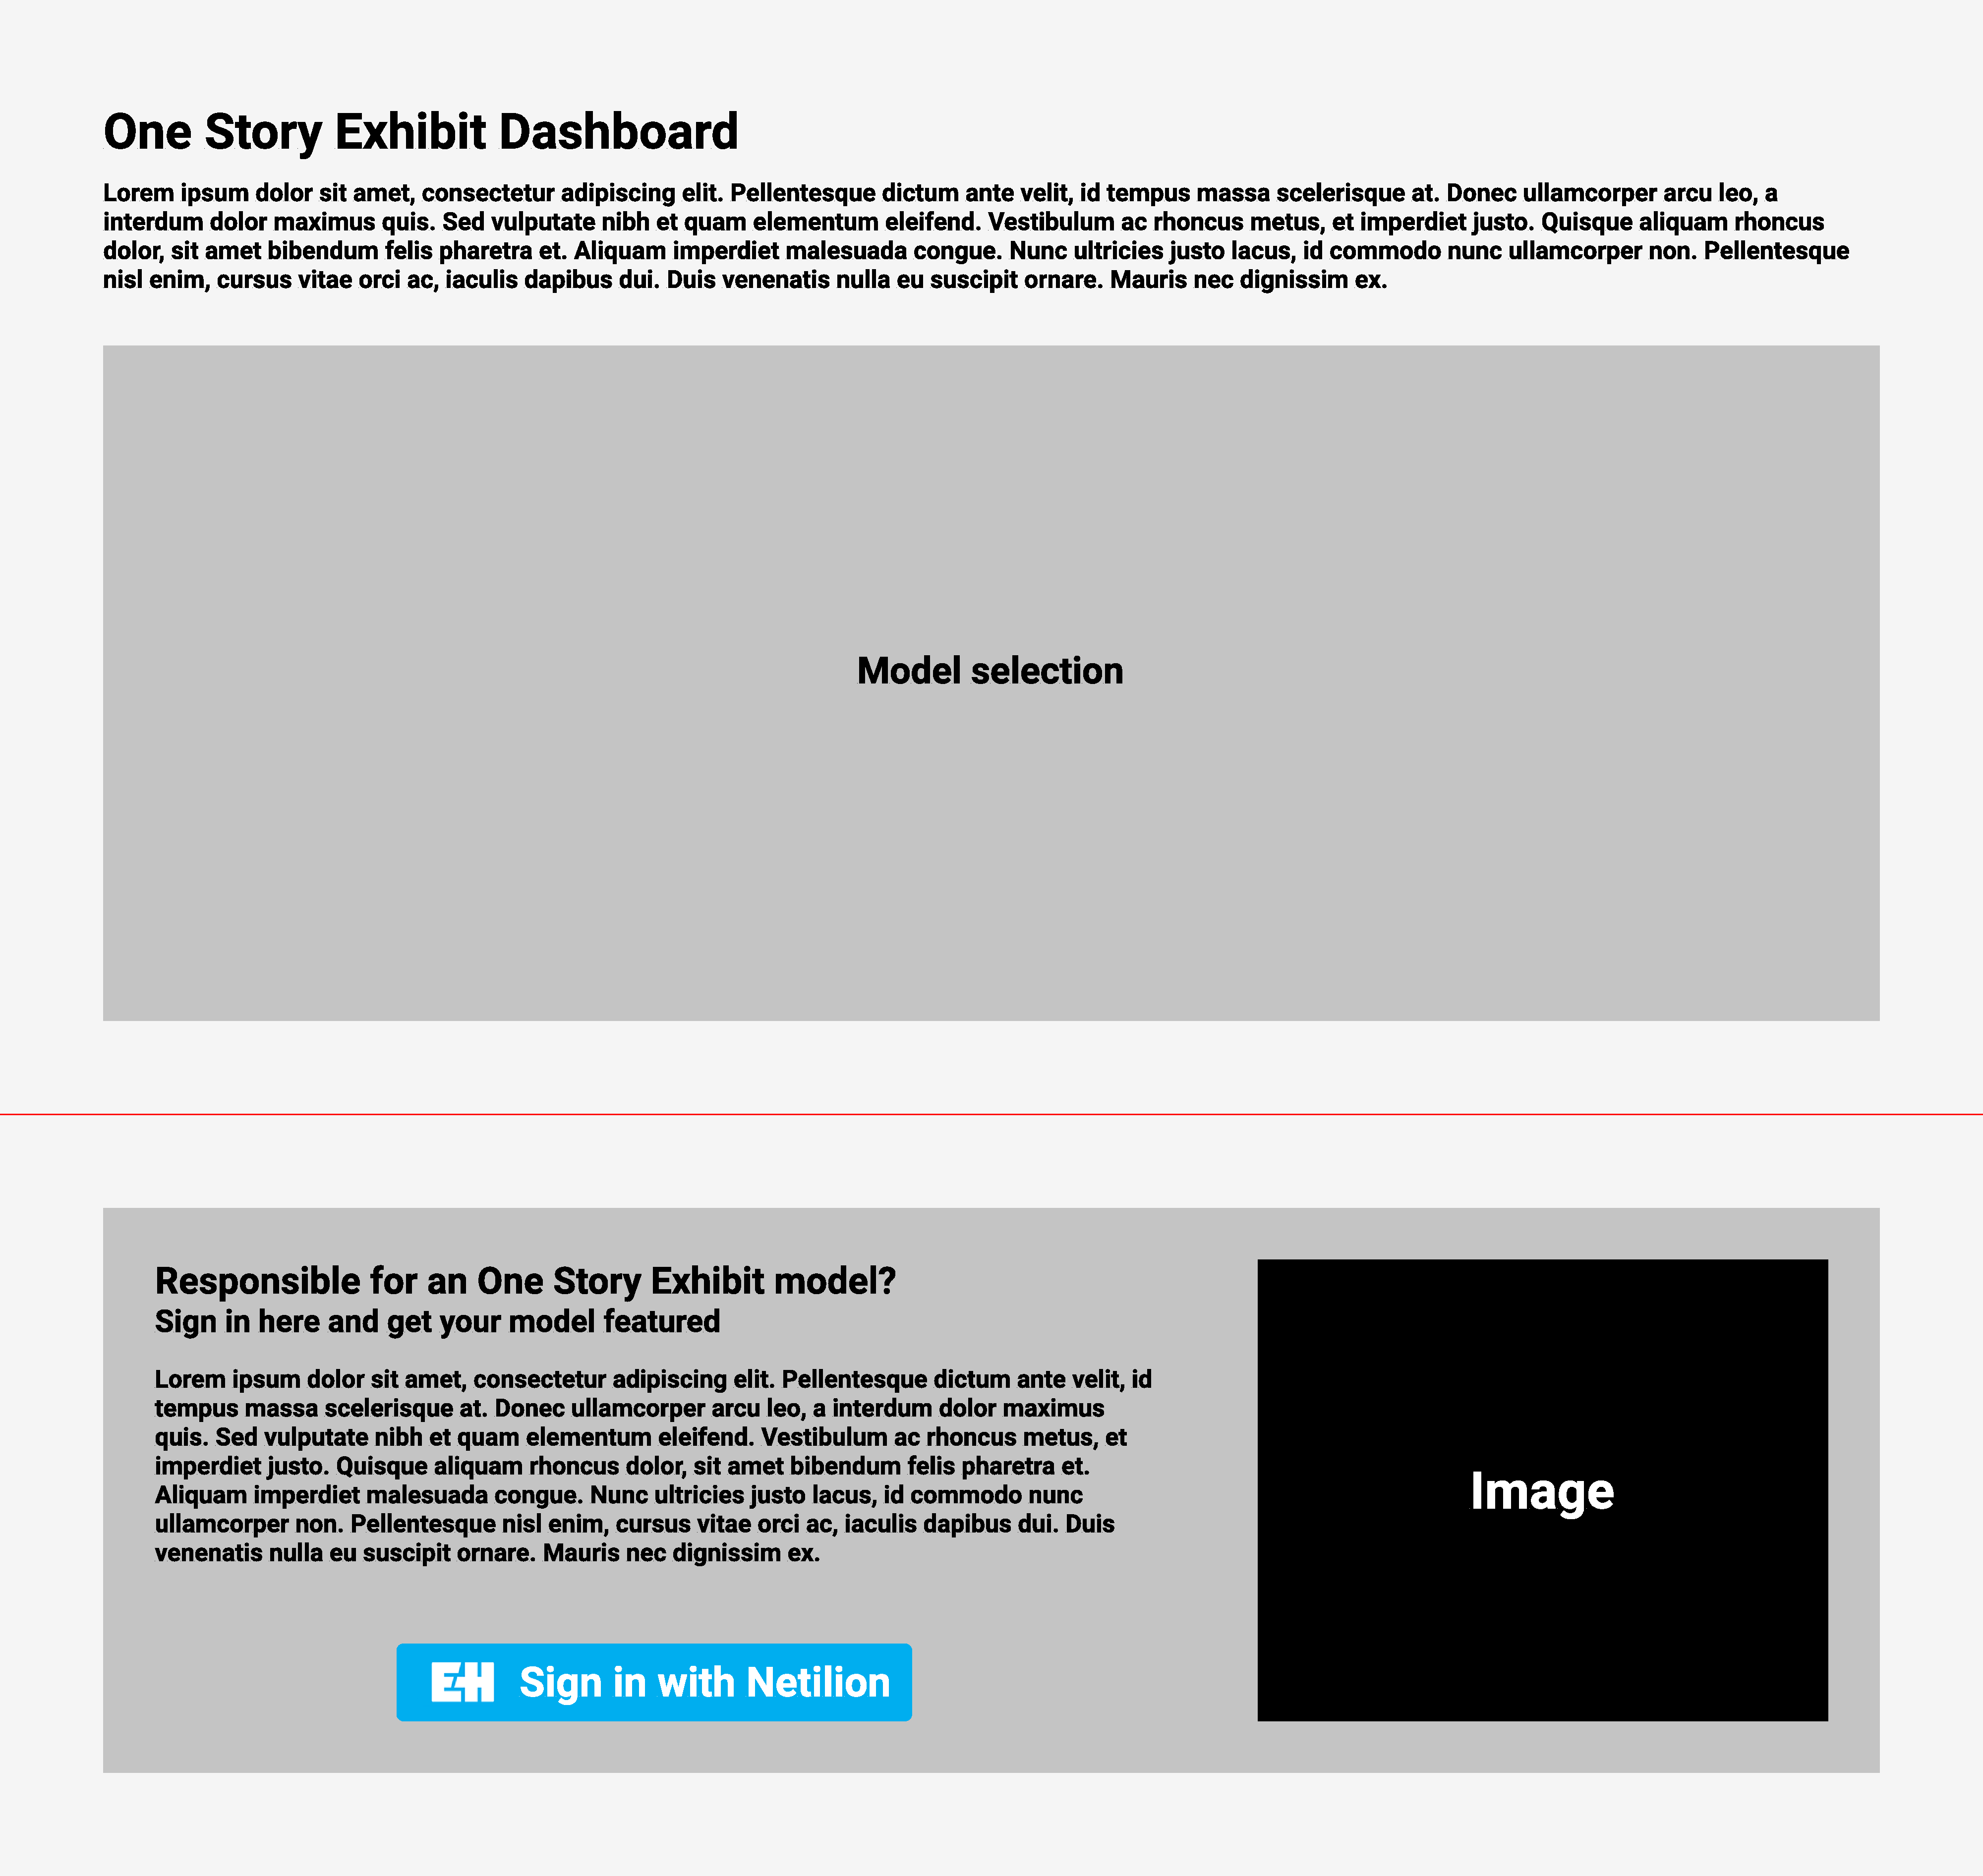
\includegraphics[width=1\textwidth]{./mockups/index/not_signed_in.pdf}
  \caption[{Mockup der Index Page}]{Mockup der Index Page}
  \label{fig:mck-index}
\end{figure}
\pagebreak
\subsection{Registration} \label{mck:registration}
\subsubsection{Fehlermeldung}
Sollte beim Loginprozess etwas schiefgehen, wird die unten dargestellte Fehlermeldung angezeigt. Dabei wird erwähnt, dass dieser Fehler sehr wahrscheinlich durch den Kandidaten geschah und nicht durch Netilion. Darunter befindet sich die Meldung, dass der User in x Sekunden wieder auf die Startseite weitergeleited wird.
\begin{figure}[H]
  \centering
  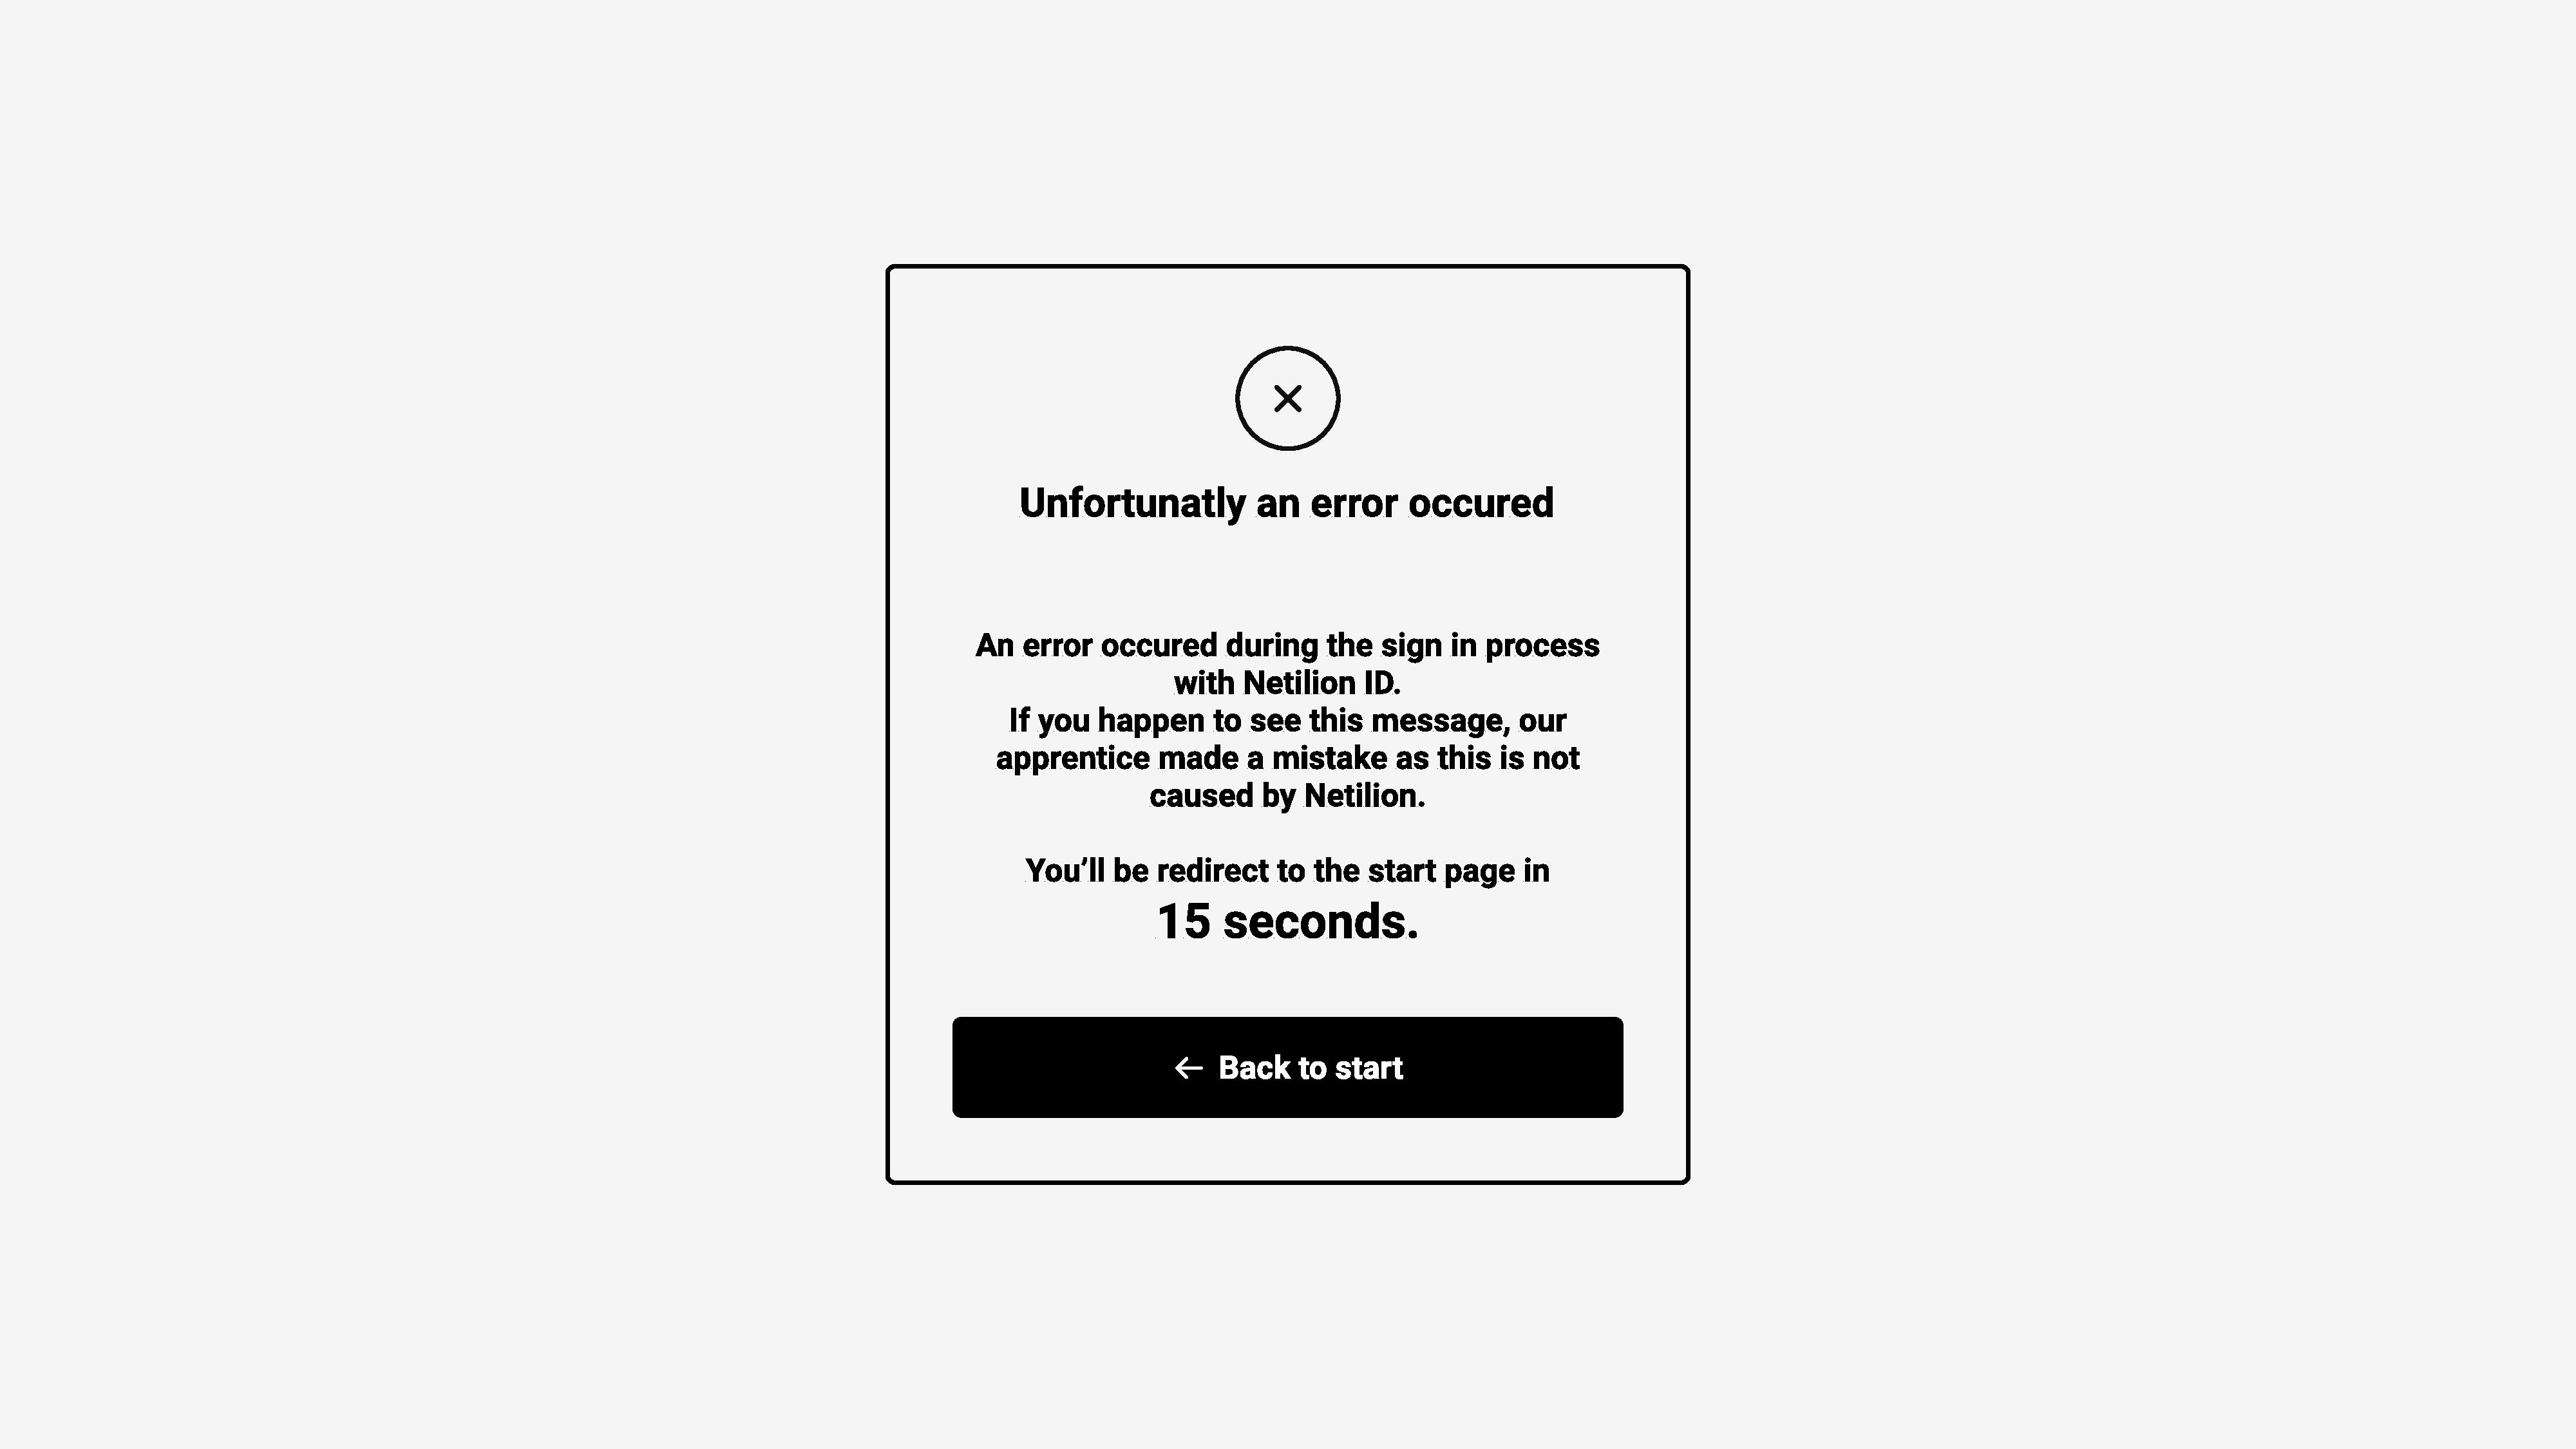
\includegraphics[width=1\textwidth]{./mockups/register/error.pdf}
  \caption[{Mockup einer Fehlermeldung}]{Mockup einer Fehlermeldung}
  \label{fig:mck-error}
\end{figure}
\pagebreak
\subsubsection{Anmeldung erfolgreich}
Diese Ansicht wird angezeigt, wenn der Loginprozess erfolgreich abläuft. Dabei wird im oberen Teil angezeigt, dass dies der Erste der insgesammt drei Schritte ist, welche für die erfolgreiche Registration benötigt werden.
\begin{figure}[H]
  \centering
  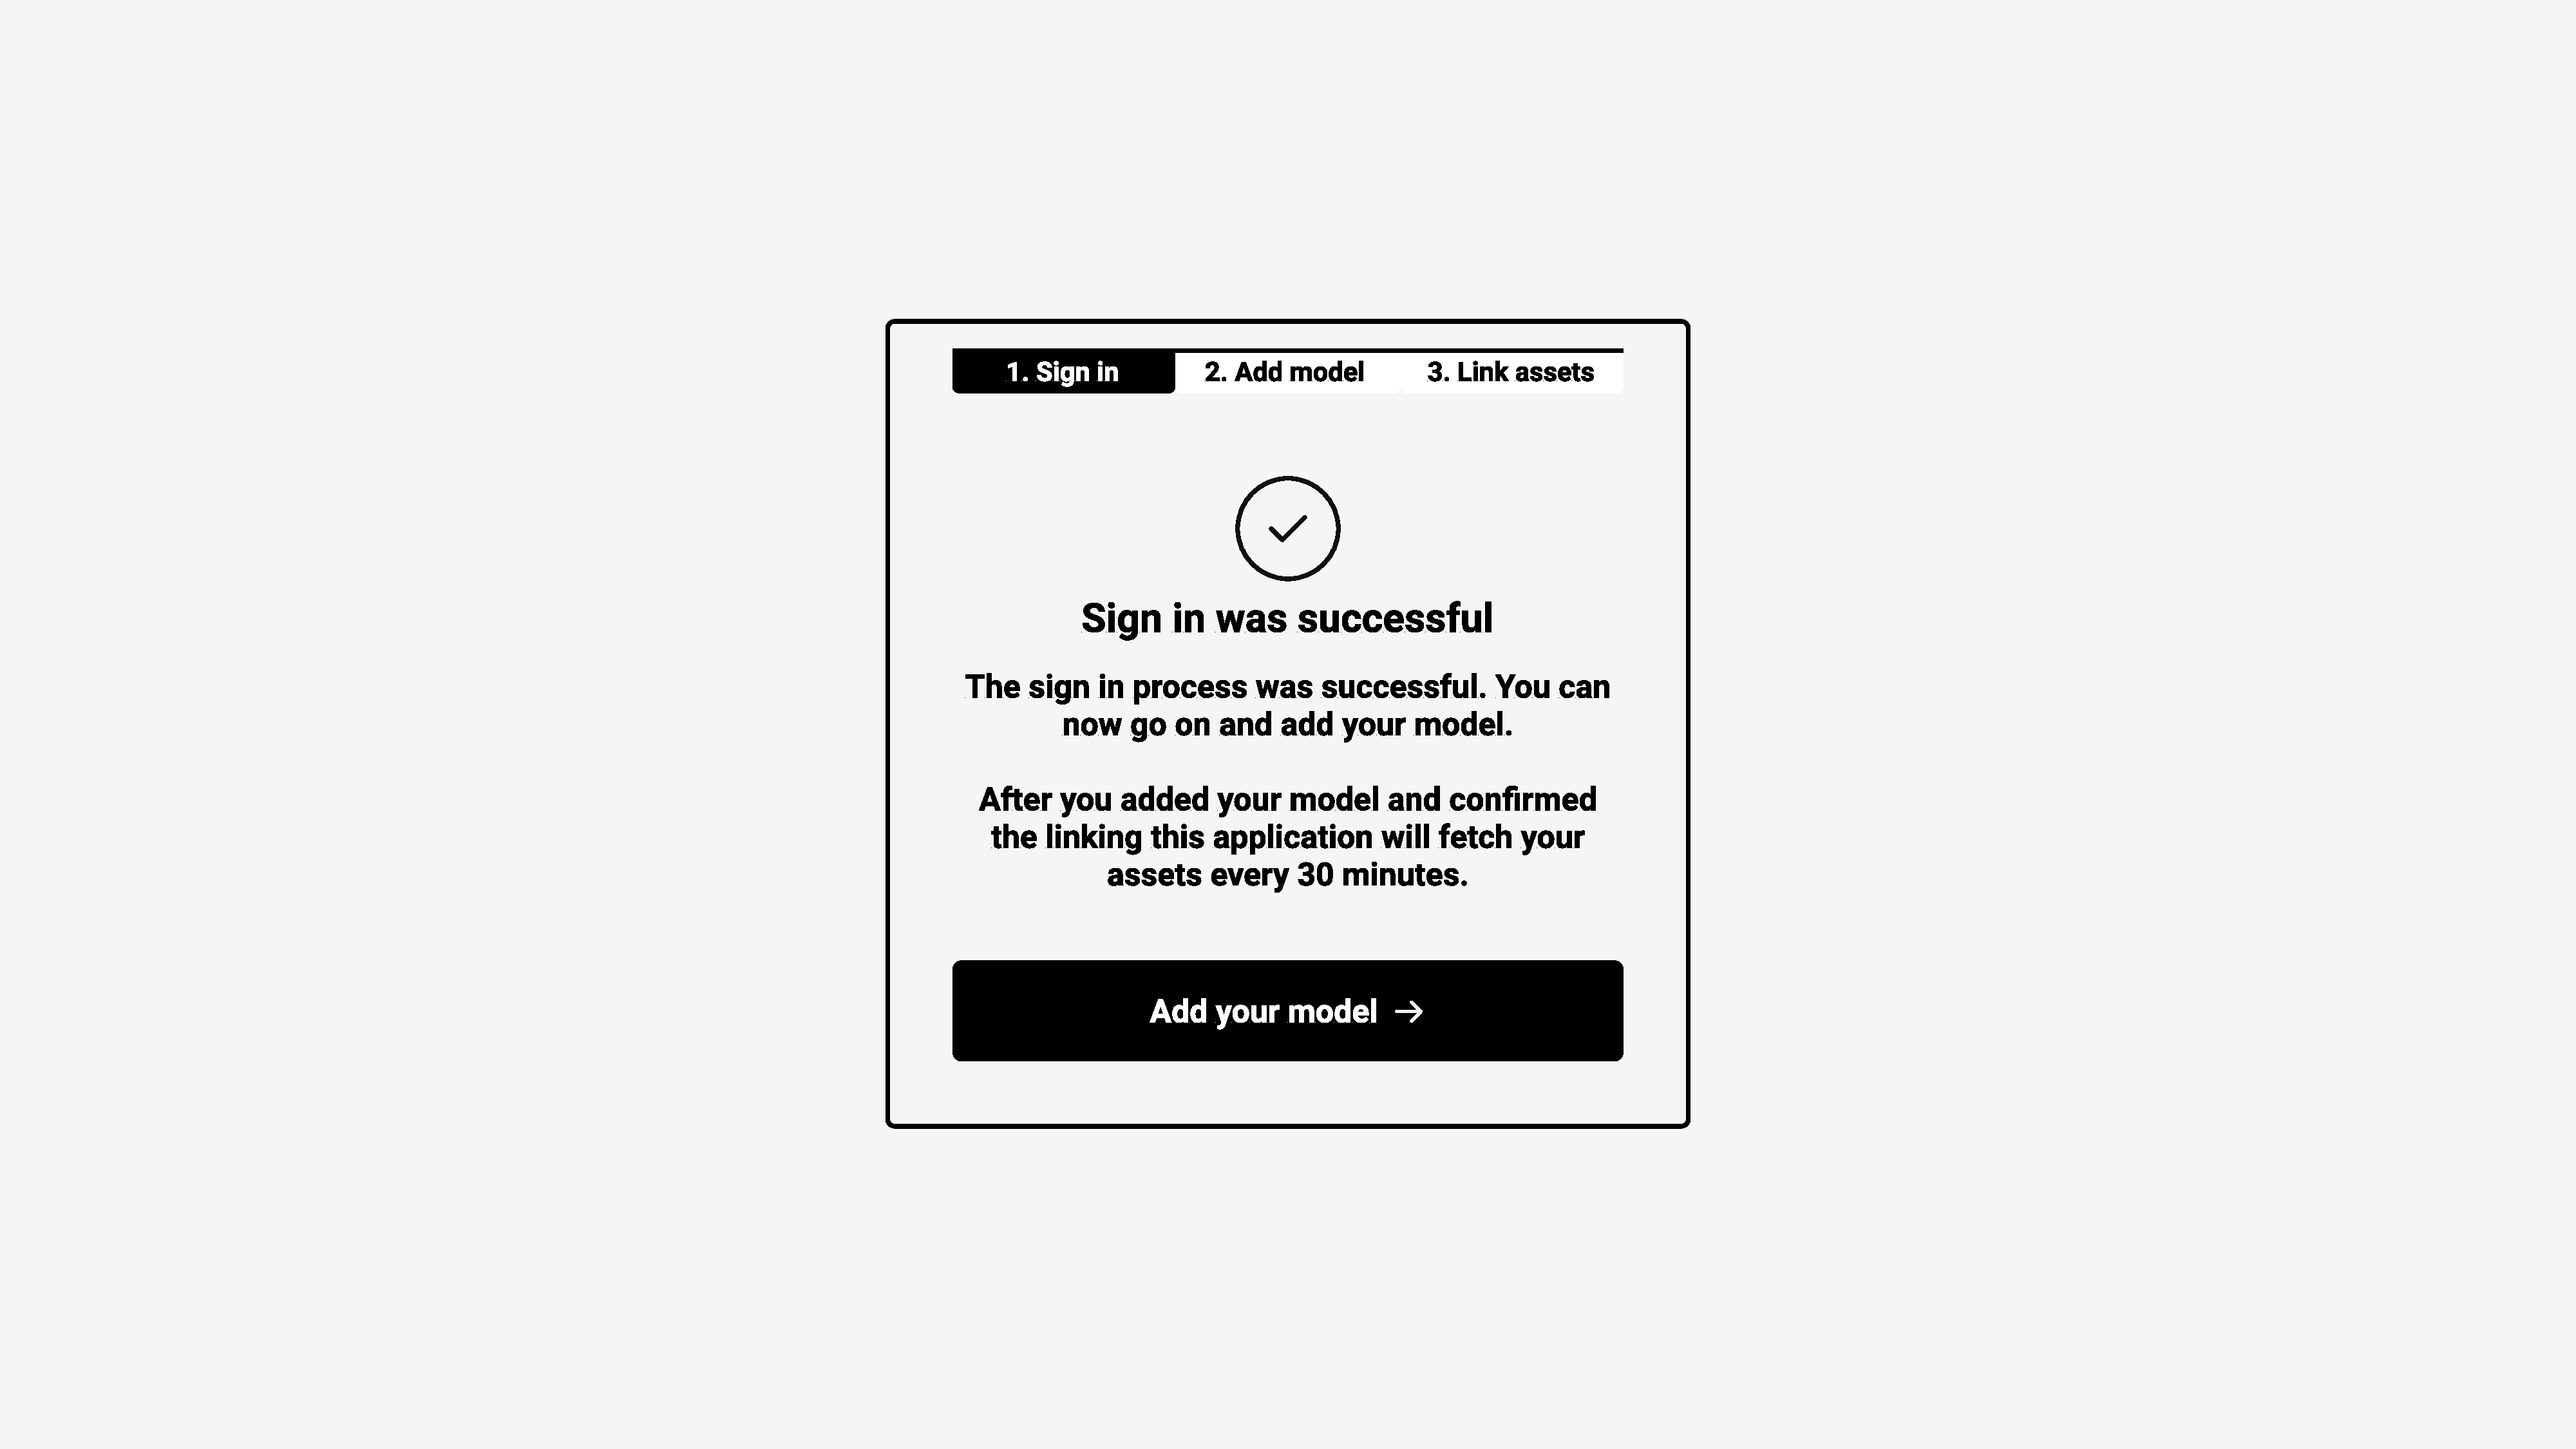
\includegraphics[width=1\textwidth]{./mockups/register/stage_1.pdf}
  \caption[{Mockup einer erfolgreichen Anmeldung}]{Mockup einer erfolgreichen Anmeldung}
  \label{fig:mck-stage_1}
\end{figure}
\pagebreak
\subsubsection{Modell registrieren}
Nun wird der OSE-Verantwortlicher darum gebeten, seinem Modell einen Namen zu geben und den Standort anzugeben, damit die User sein Modell dann über die Index Page finden können.
\begin{figure}[H]
  \centering
  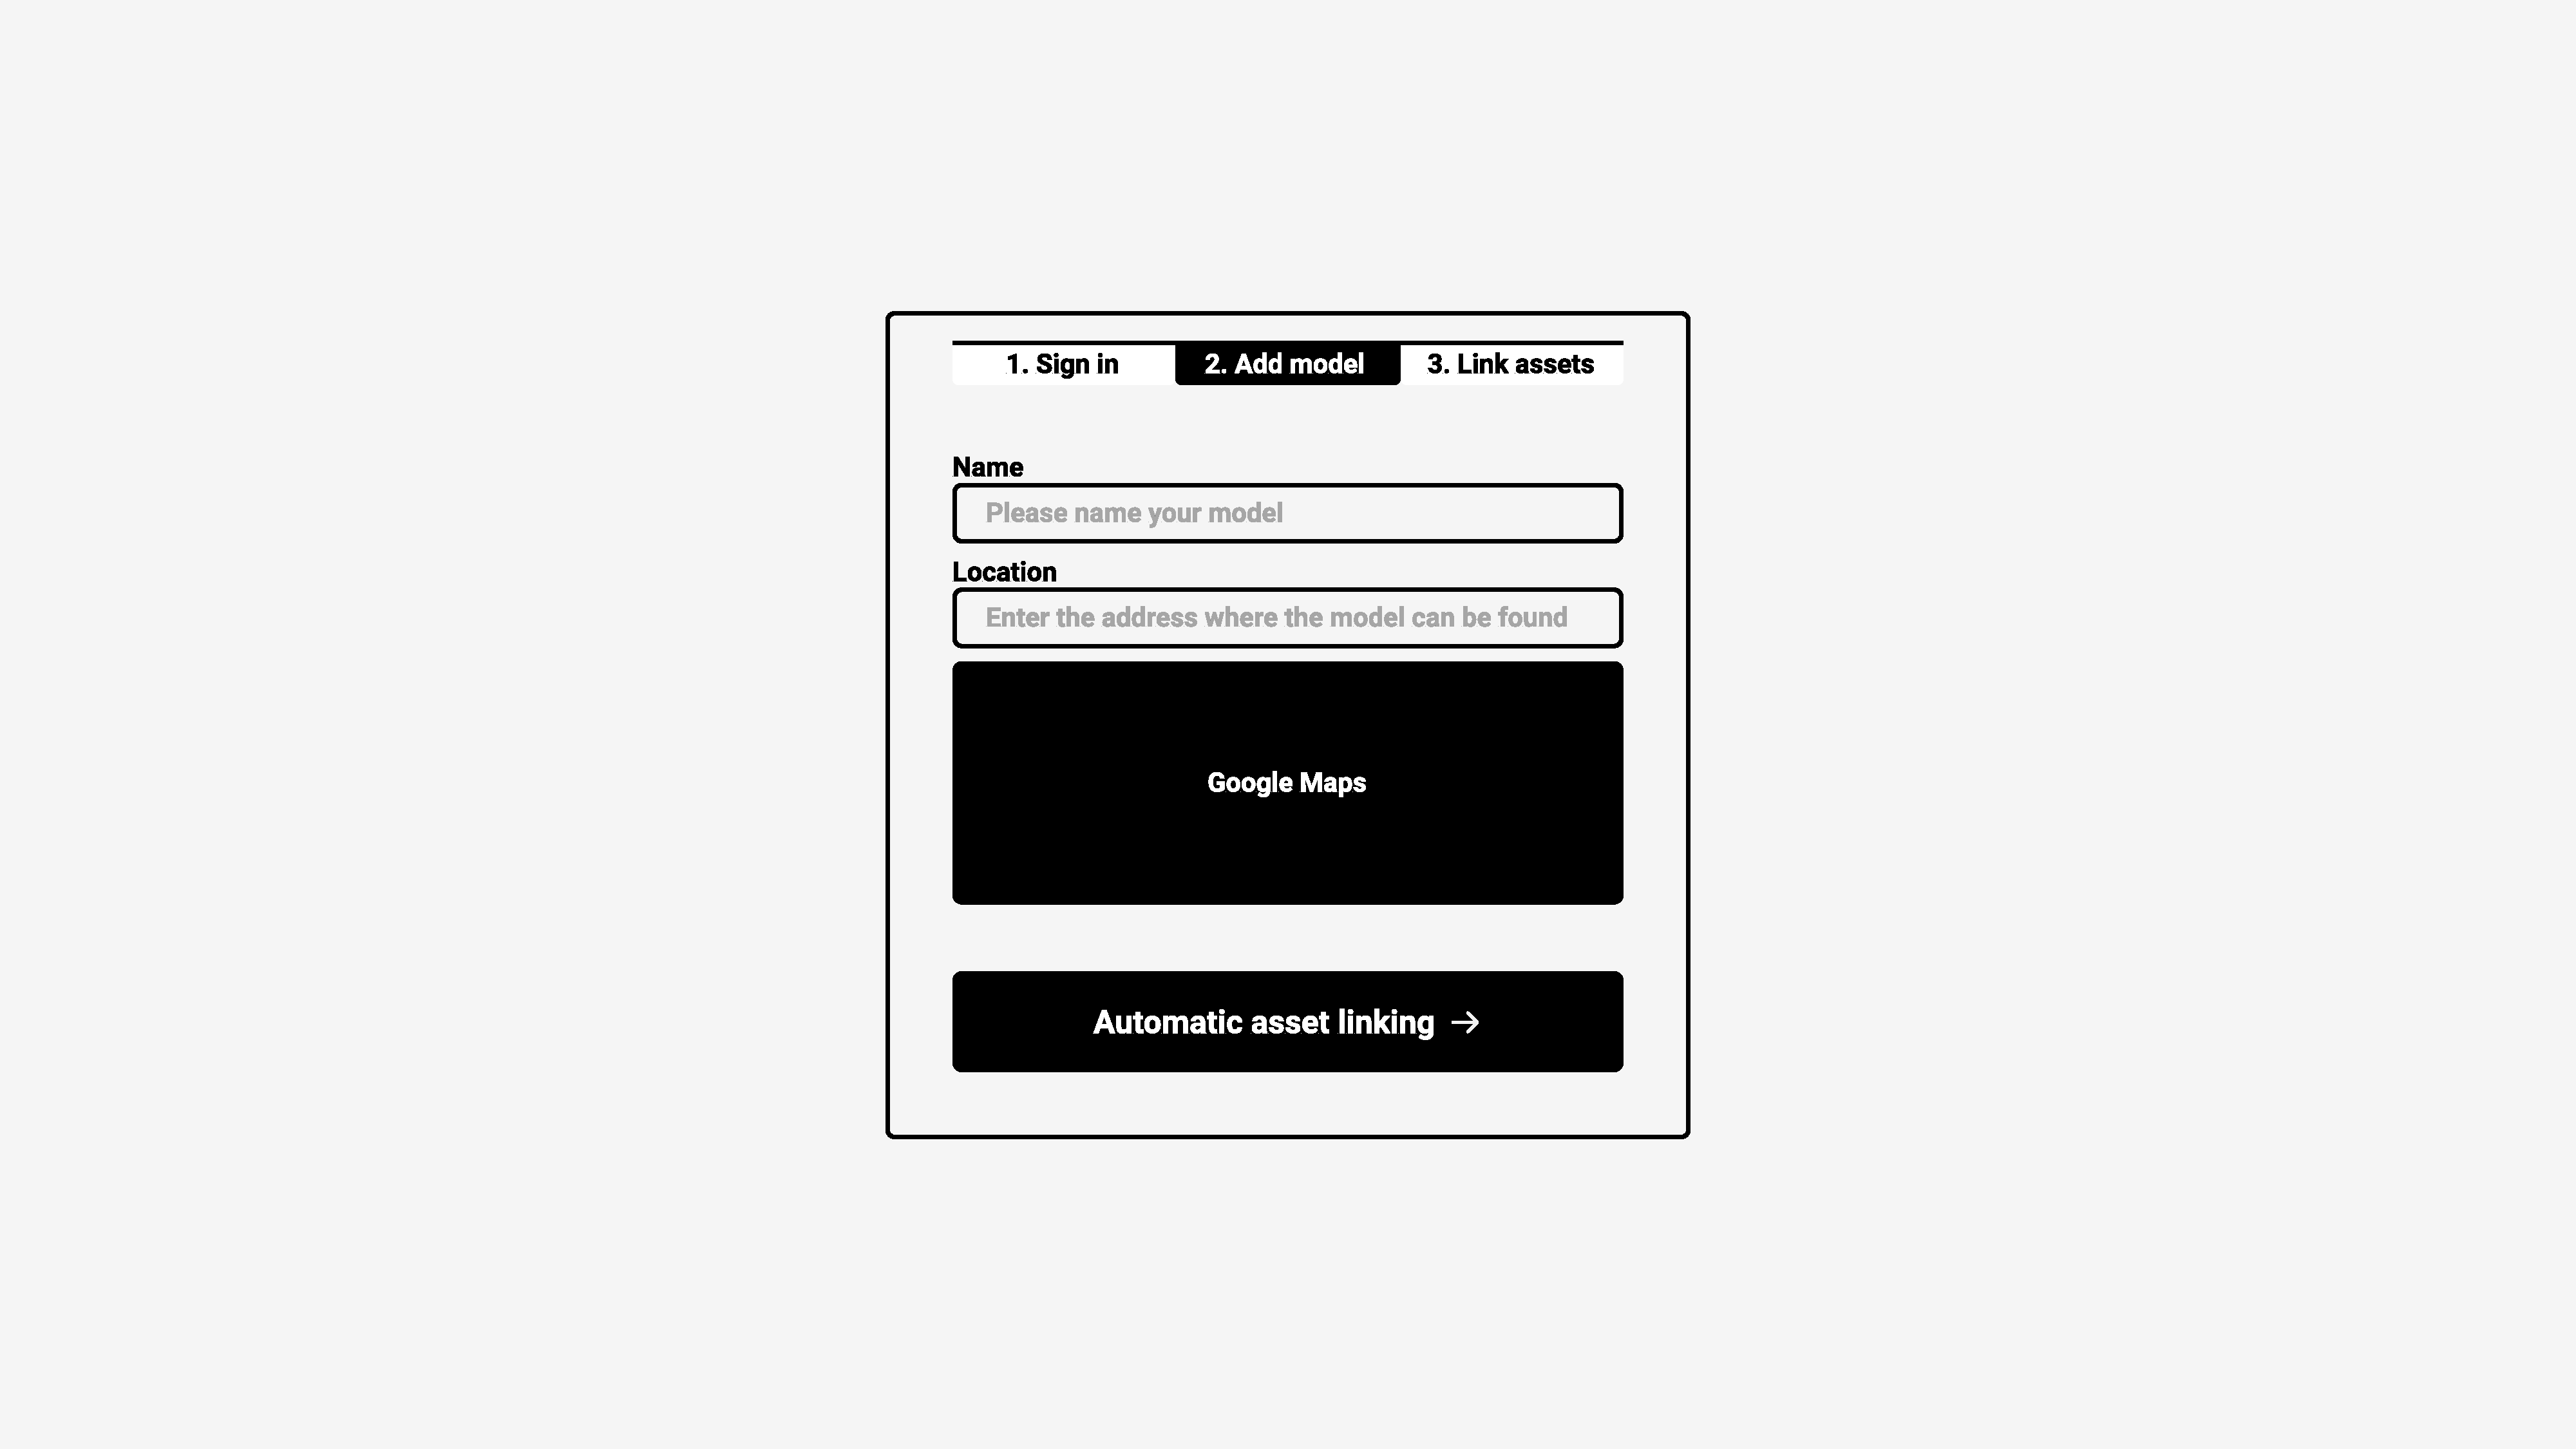
\includegraphics[width=1\textwidth]{./mockups/register/stage_2.pdf}
  \caption[{Mockup der Registration}]{Mockup der Registration}
  \label{fig:mck-stage_2}
\end{figure}
\pagebreak
\subsubsection{Asset verlinkung}
Der letzte Schritt der Registrierung ist das Verlinken der Assets mit den Meshes des 3D Modells. Da dies automatisch geschieht, wird der User an dieser stelle gebeten zu warten, bis der Prozess abgeschlossen ist.
\begin{figure}[H]
  \centering
  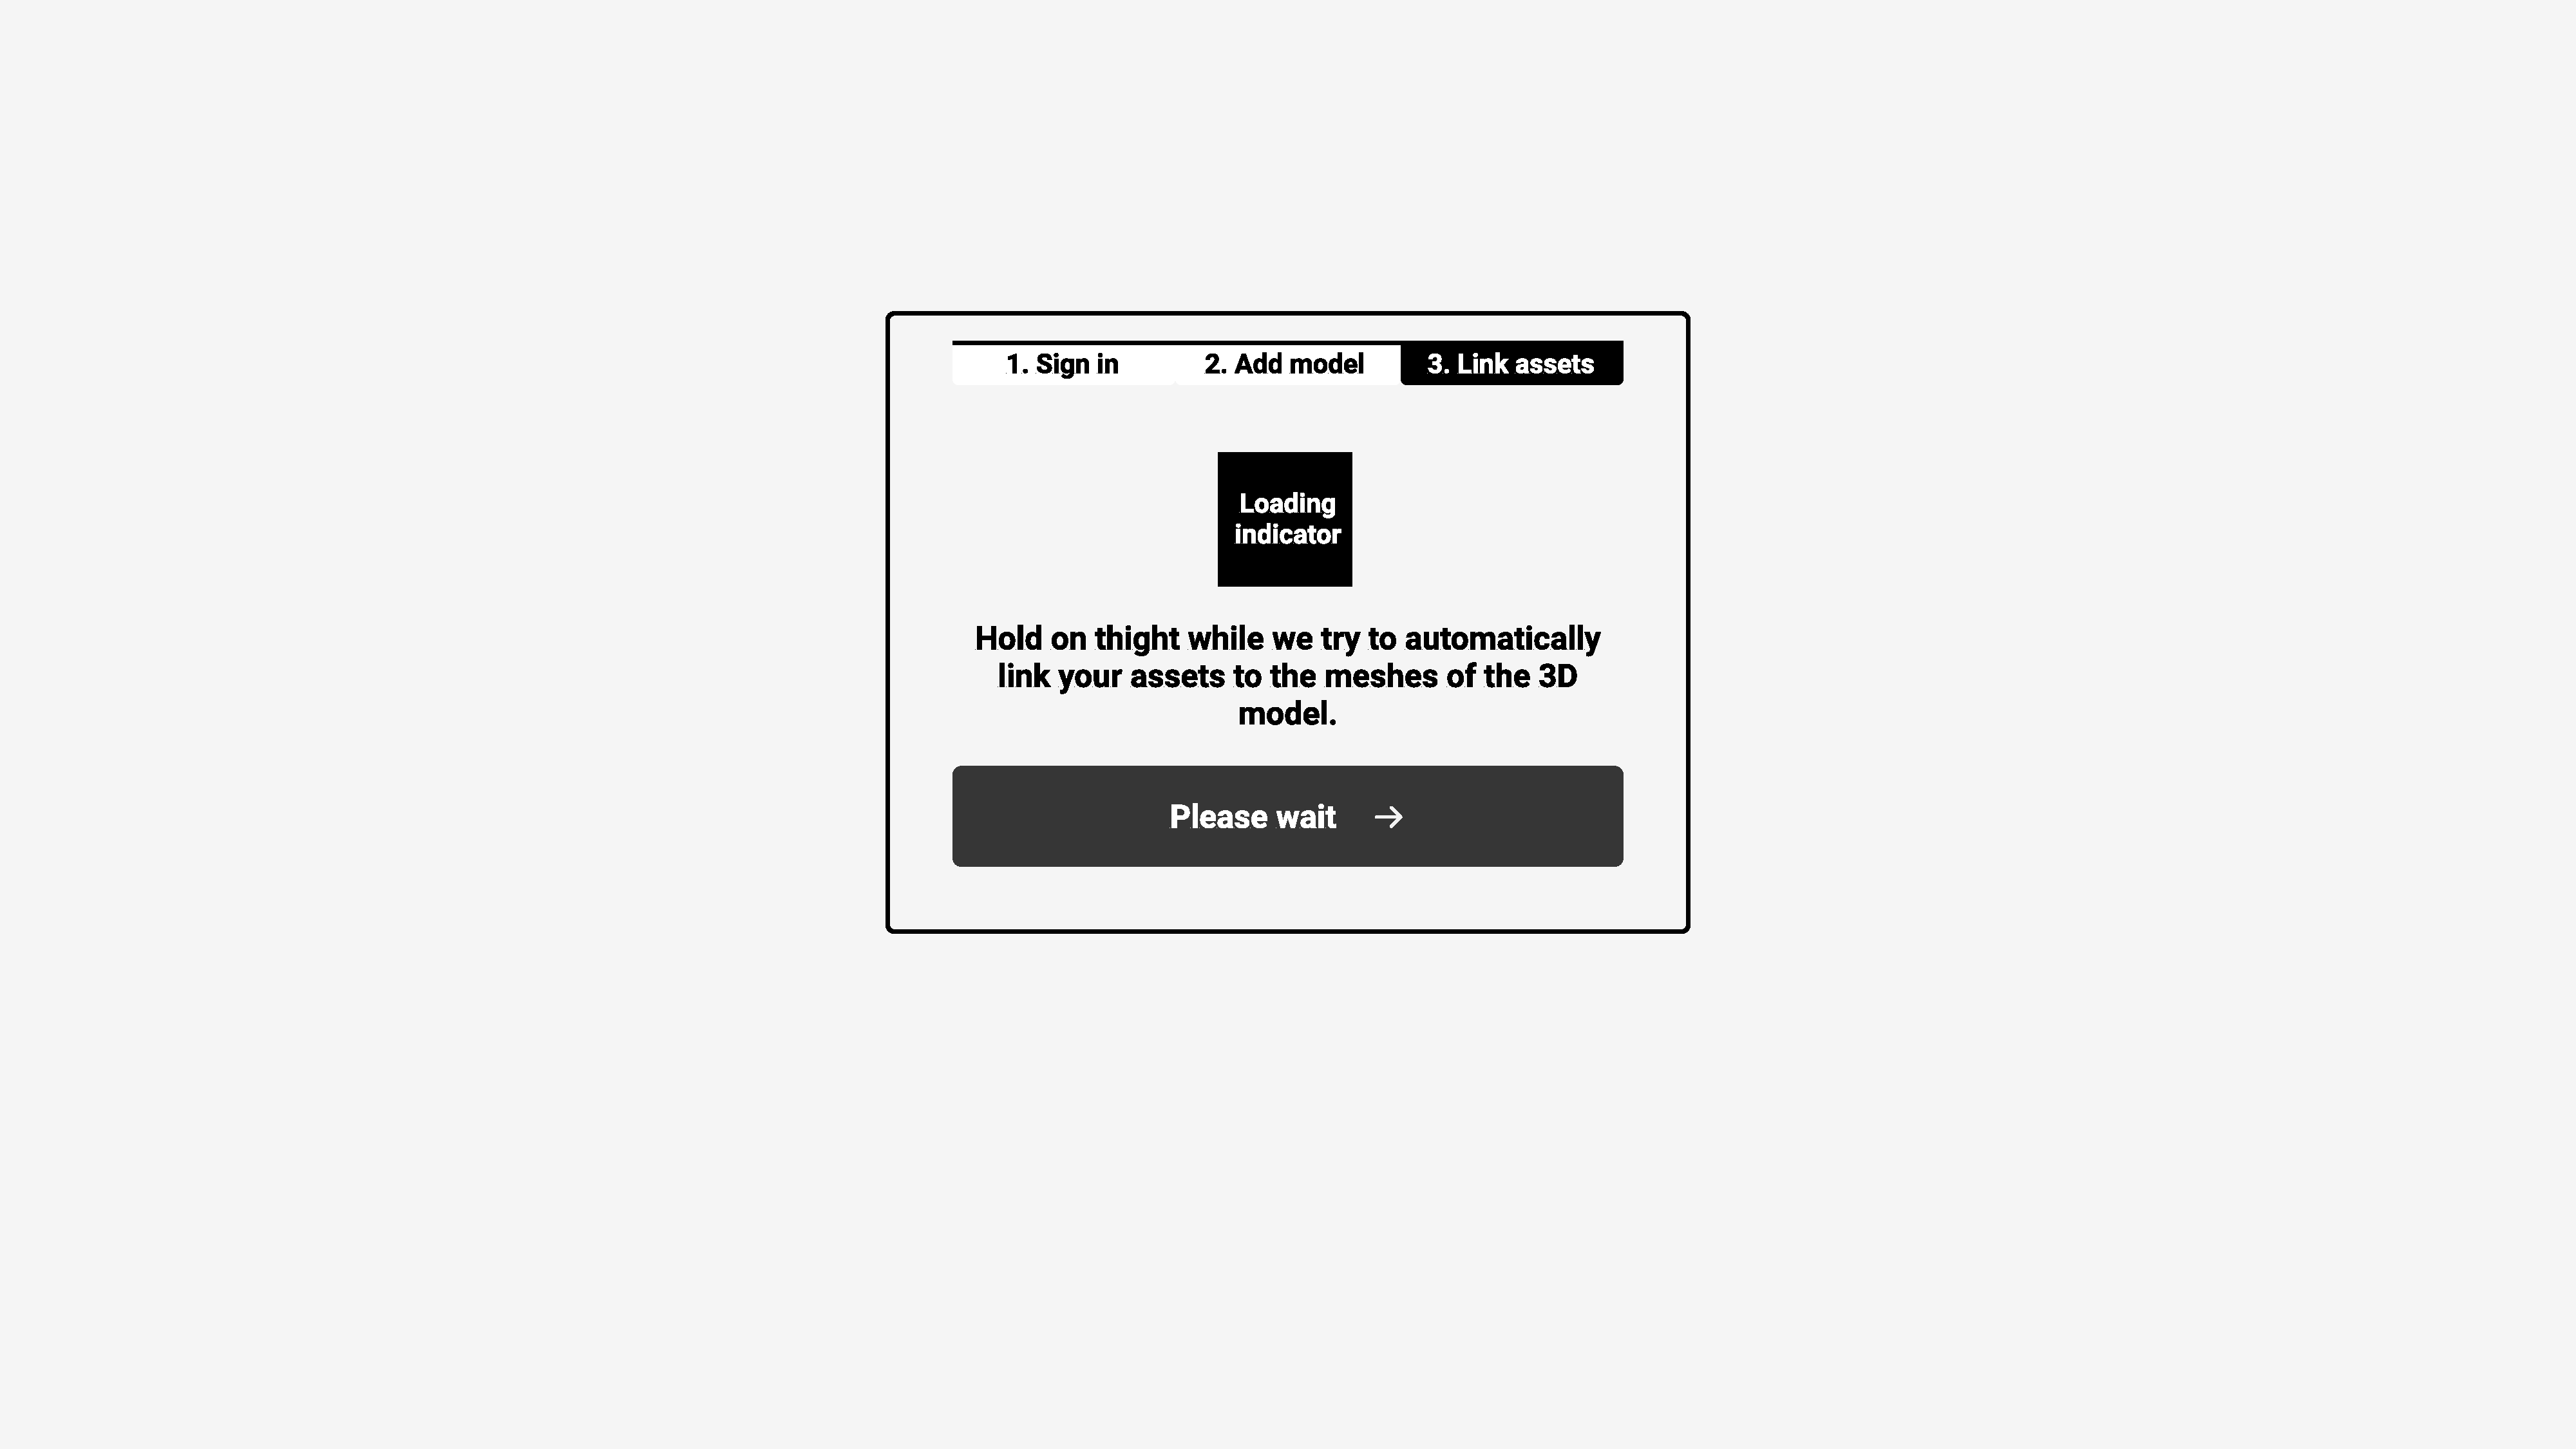
\includegraphics[width=1\textwidth]{./mockups/register/stage_3.pdf}
  \caption[{Mockup der Asset verlinkung}]{Mockup der Asset verlinkung}
  \label{fig:mck-stage_3}
\end{figure}
\pagebreak
\subsubsection{Asset verlinkung fehlgeschlagen}
Konnten nicht alle Assets verlinkt werden, wird dieses Fenster angezeigt. Es erklärt dem User was geschah und das er die Verlinkung im nächsten Schritt manuel anpassen kann.
\begin{figure}[H]
  \centering
  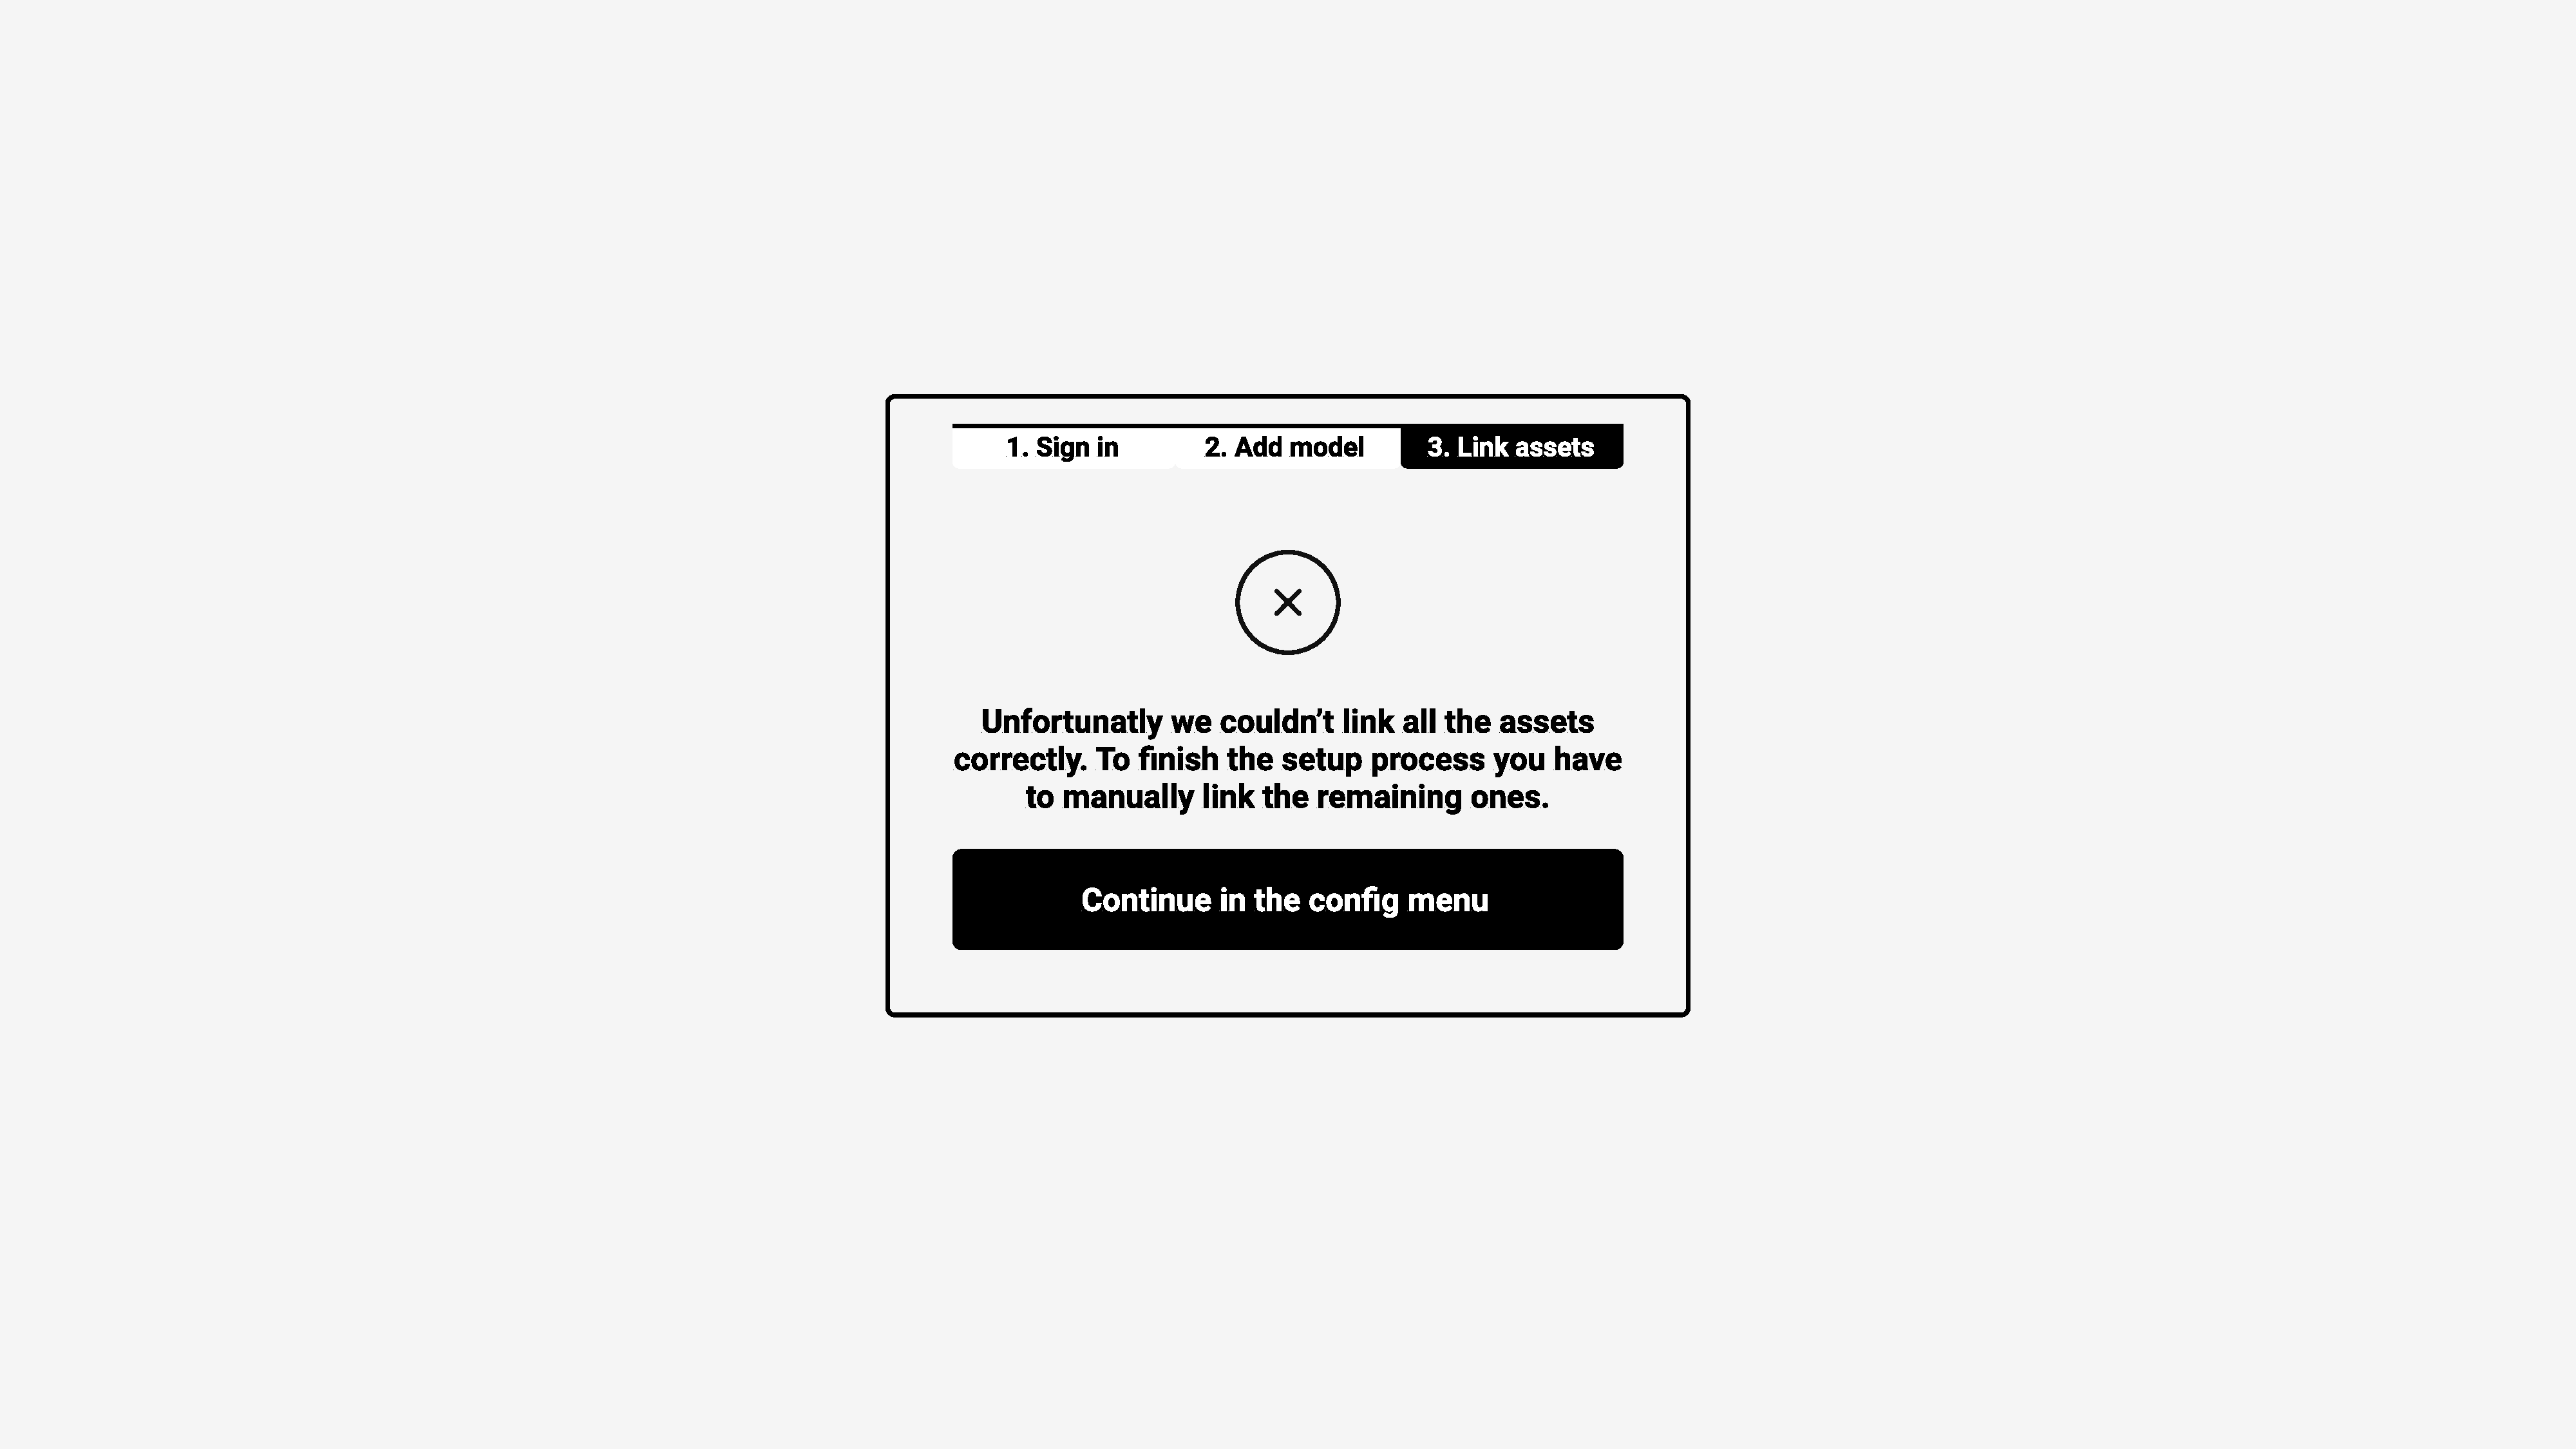
\includegraphics[width=1\textwidth]{./mockups/register/redirect.pdf}
  \caption[{Mockup einer fehlgeschlagenen Verlinkung}]{Mockup einer fehlgeschlagenen Verlinkung}
  \label{fig:mck-redirect}
\end{figure}
\pagebreak
\subsubsection{Asset verlinkung erfolgreich}
Konnten alle Assets verlinkt werden, wird dieses Fenster angezeigt. Es informiert den User, dass der Registrationsprozess hiermit abgeschlossen ist. Mit dem Knopf am unteren Rand wird er ausgeloggt und kehrt zur Startseite zurück.
\begin{figure}[H]
  \centering
  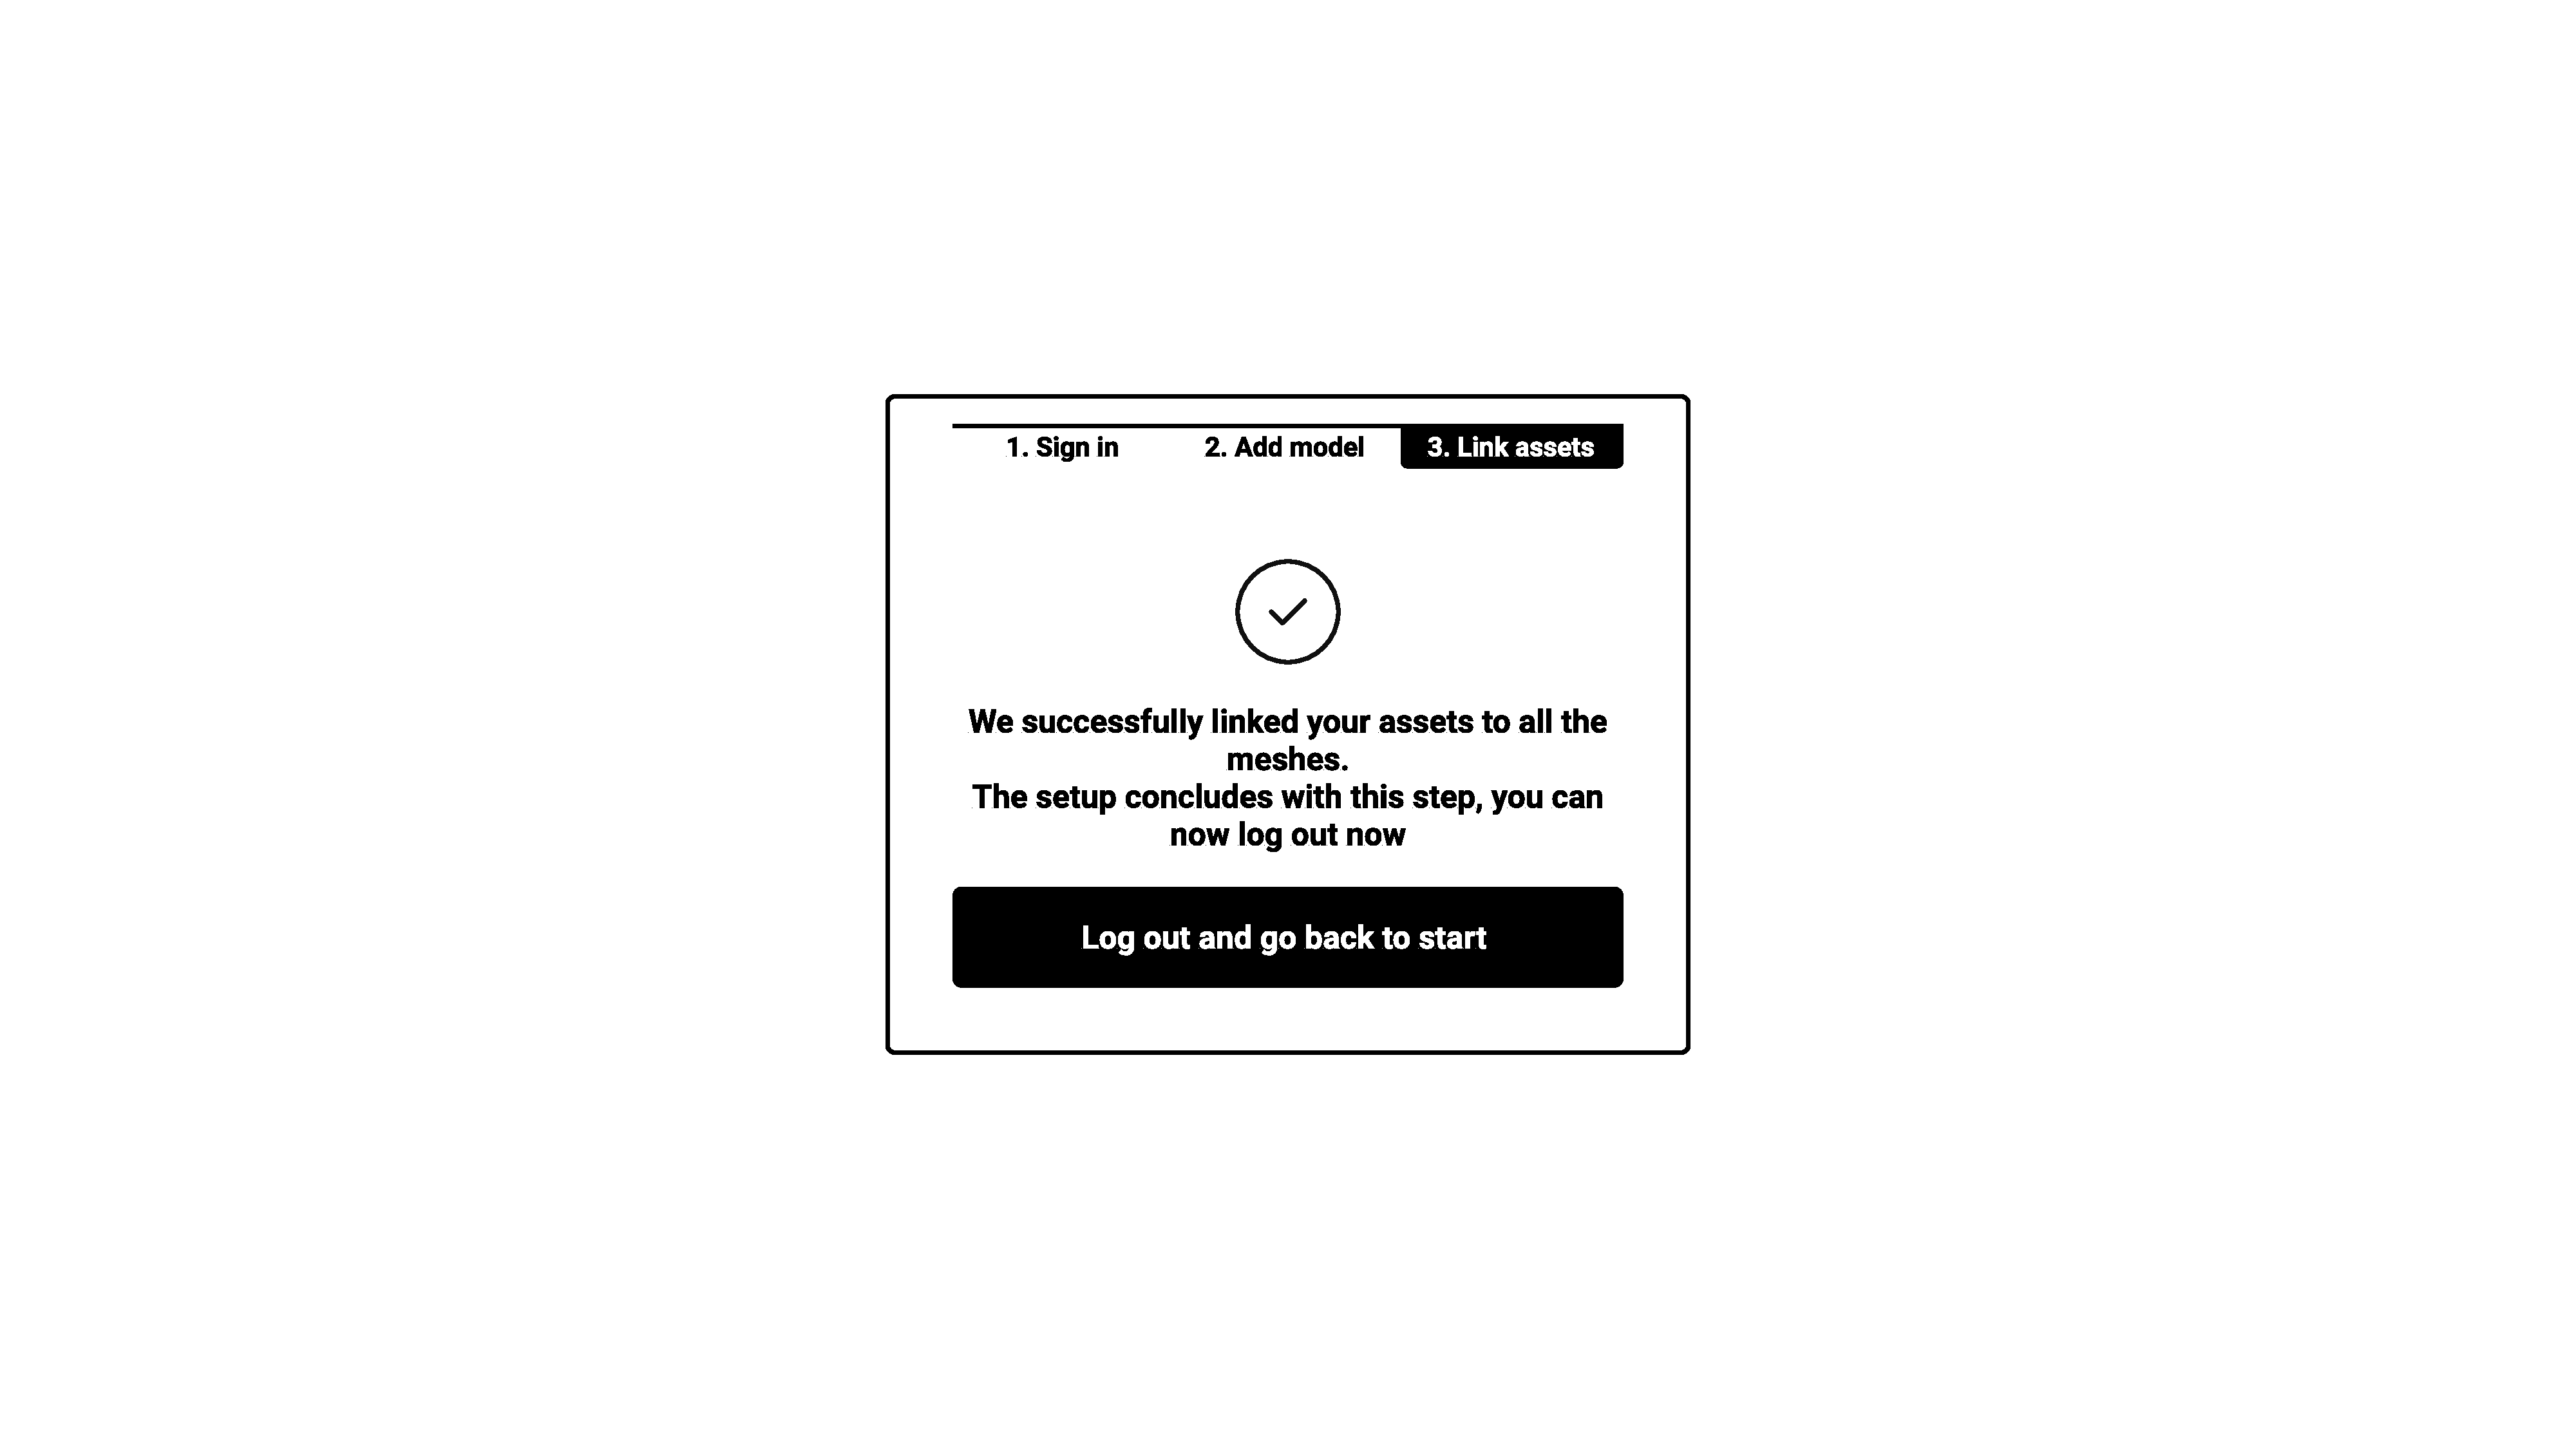
\includegraphics[width=1\textwidth]{./mockups/register/all_success.pdf}
  \caption[{Mockup einer erfolgreichen Verlinkung}]{Mockup einer erfolgreichen Verlinkung}
  \label{fig:mck-all_success}
\end{figure}
\pagebreak
\subsection{Einstellungsmenü}
\subsubsection{Modelleinstellungen}
Nachfolgend ist ein Design für die Modelleinstellungsseite. Hier kann der OSE Verantwortlicher den Namen und die Beschreibung des Modells ändern.
\begin{figure}[H]
  \centering
  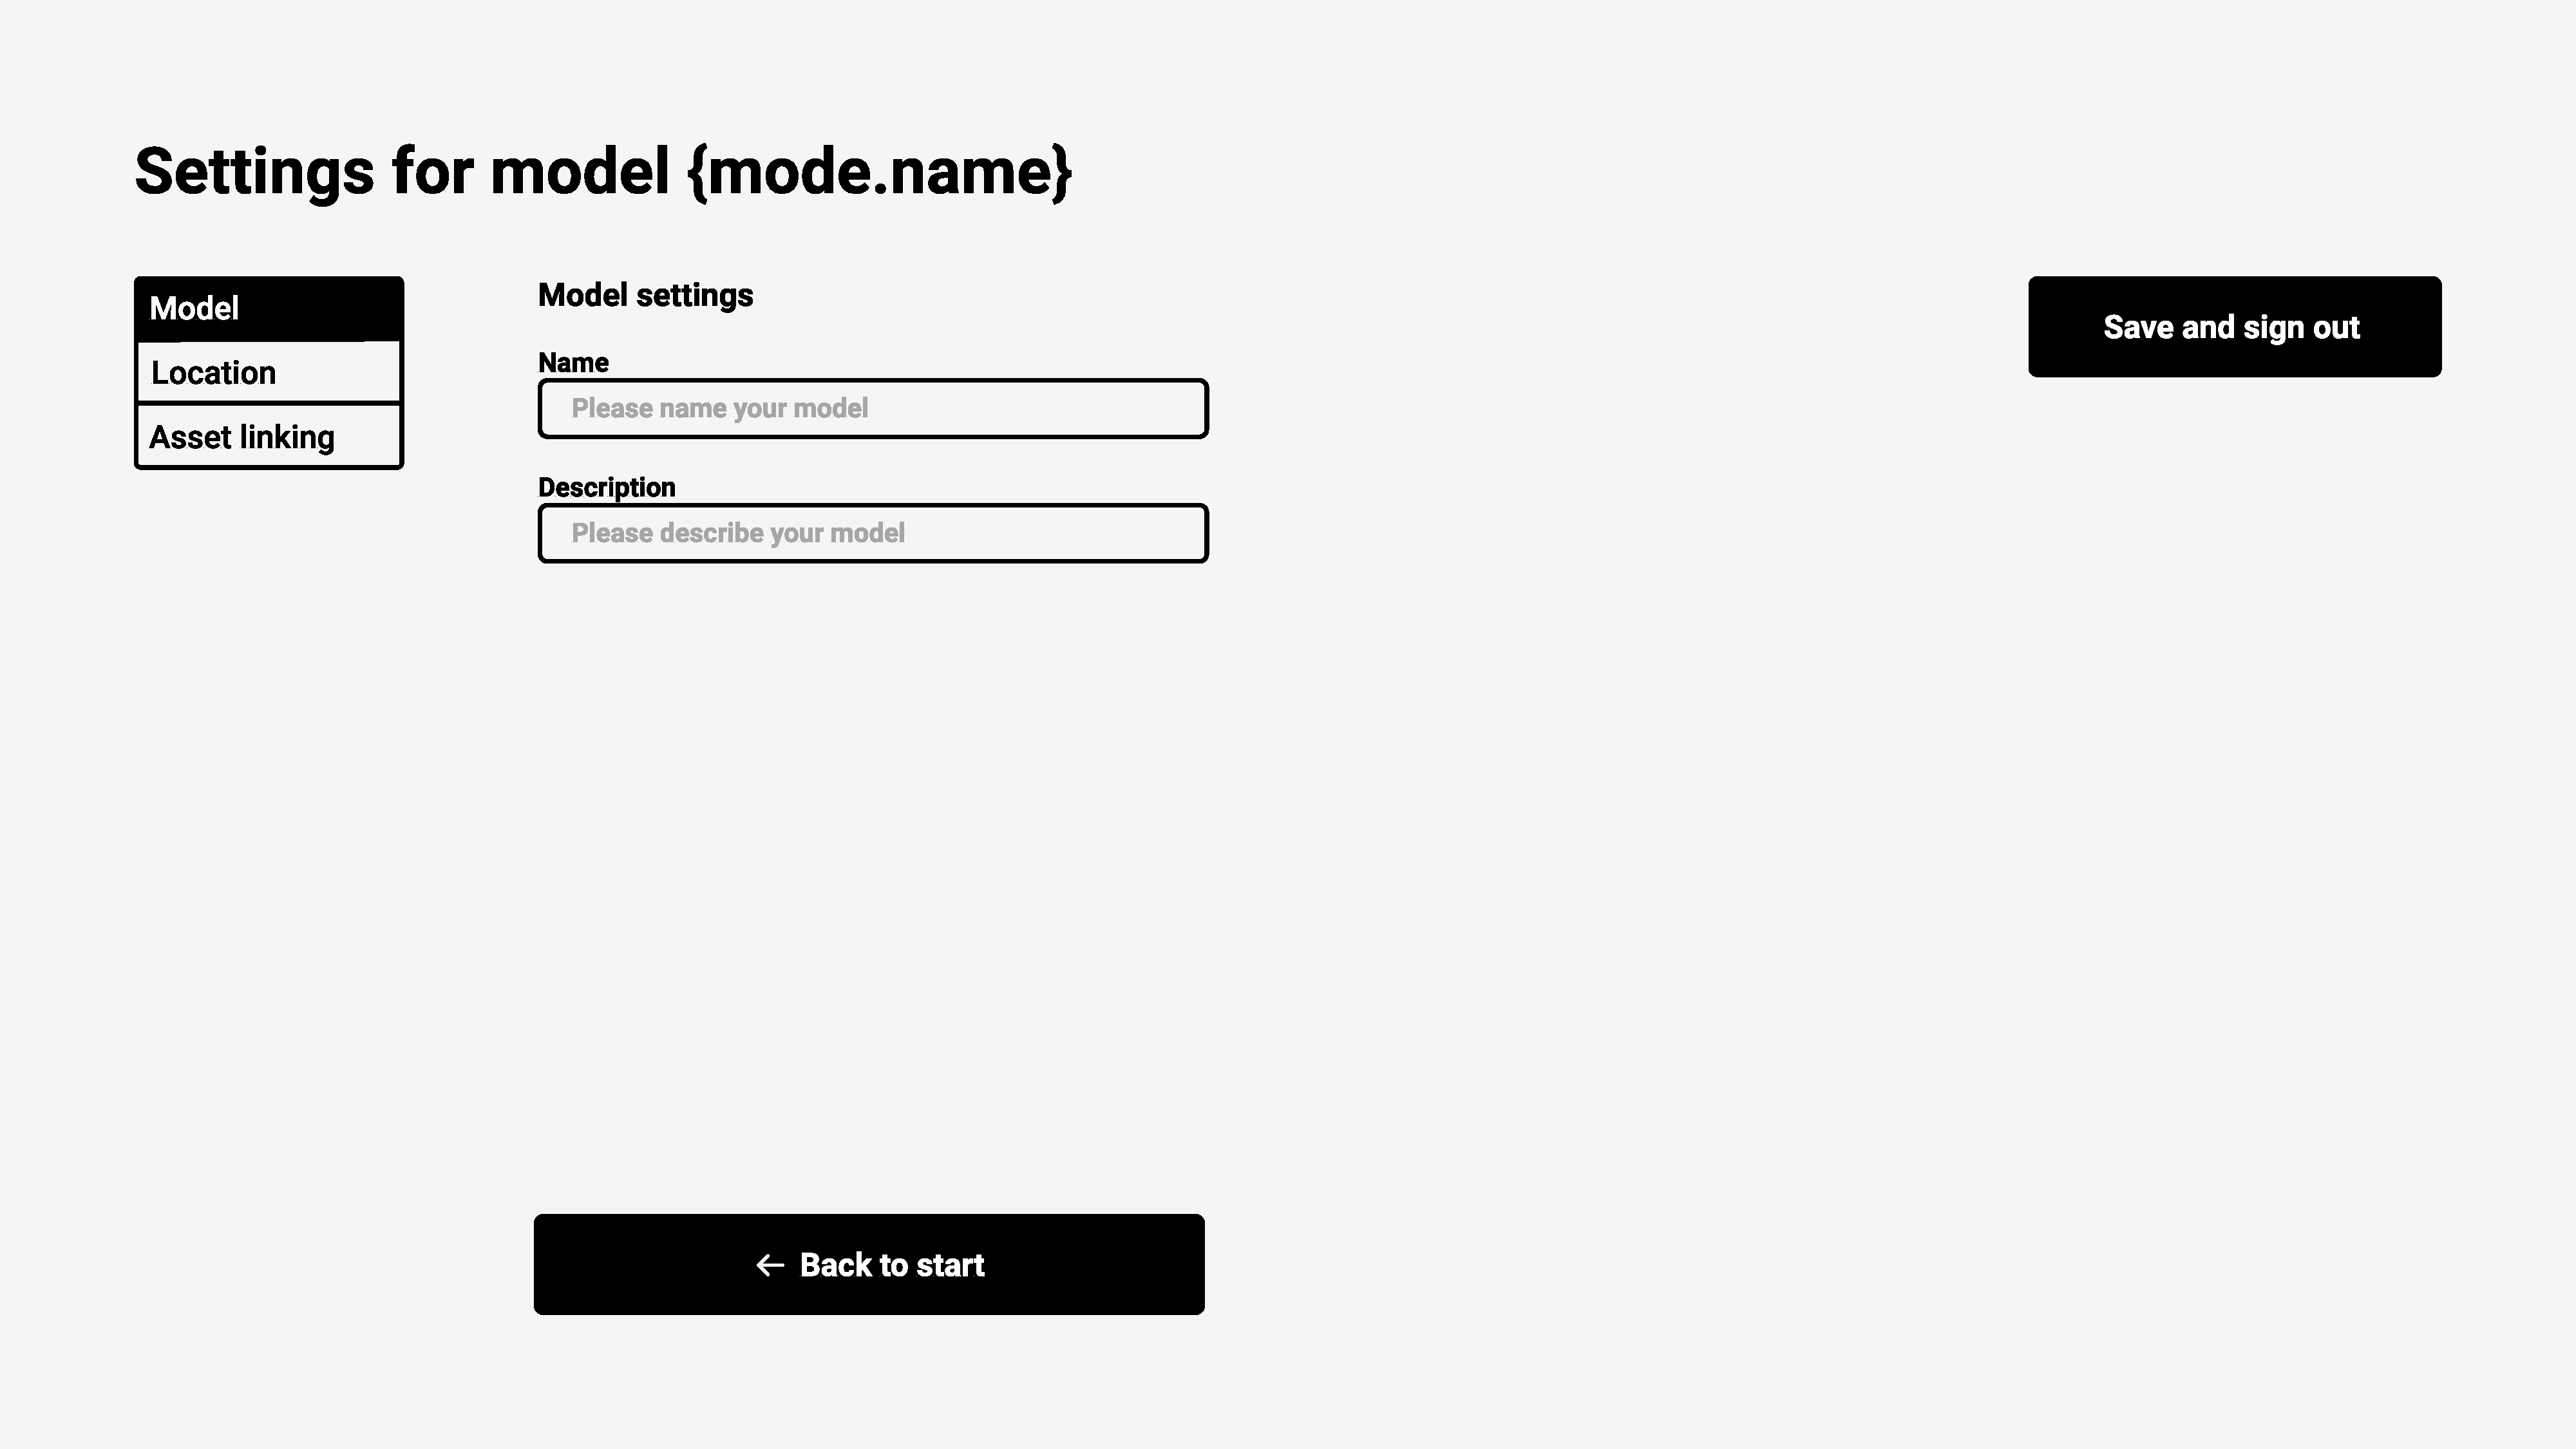
\includegraphics[width=1\textwidth]{./mockups/settings/Model.pdf}
  \caption[{Mockup des Modelleinstellungsmenü}]{Mockup des Modelleinstellungsmenü}
  \label{fig:mck-model}
\end{figure}
\pagebreak
\subsubsection{Standorteinstellungen}
Dies ist das Design für die Standortseinstellungsseite. Hier kann der Standort im nachhinein verändert werden.
\begin{figure}[H]
  \centering
  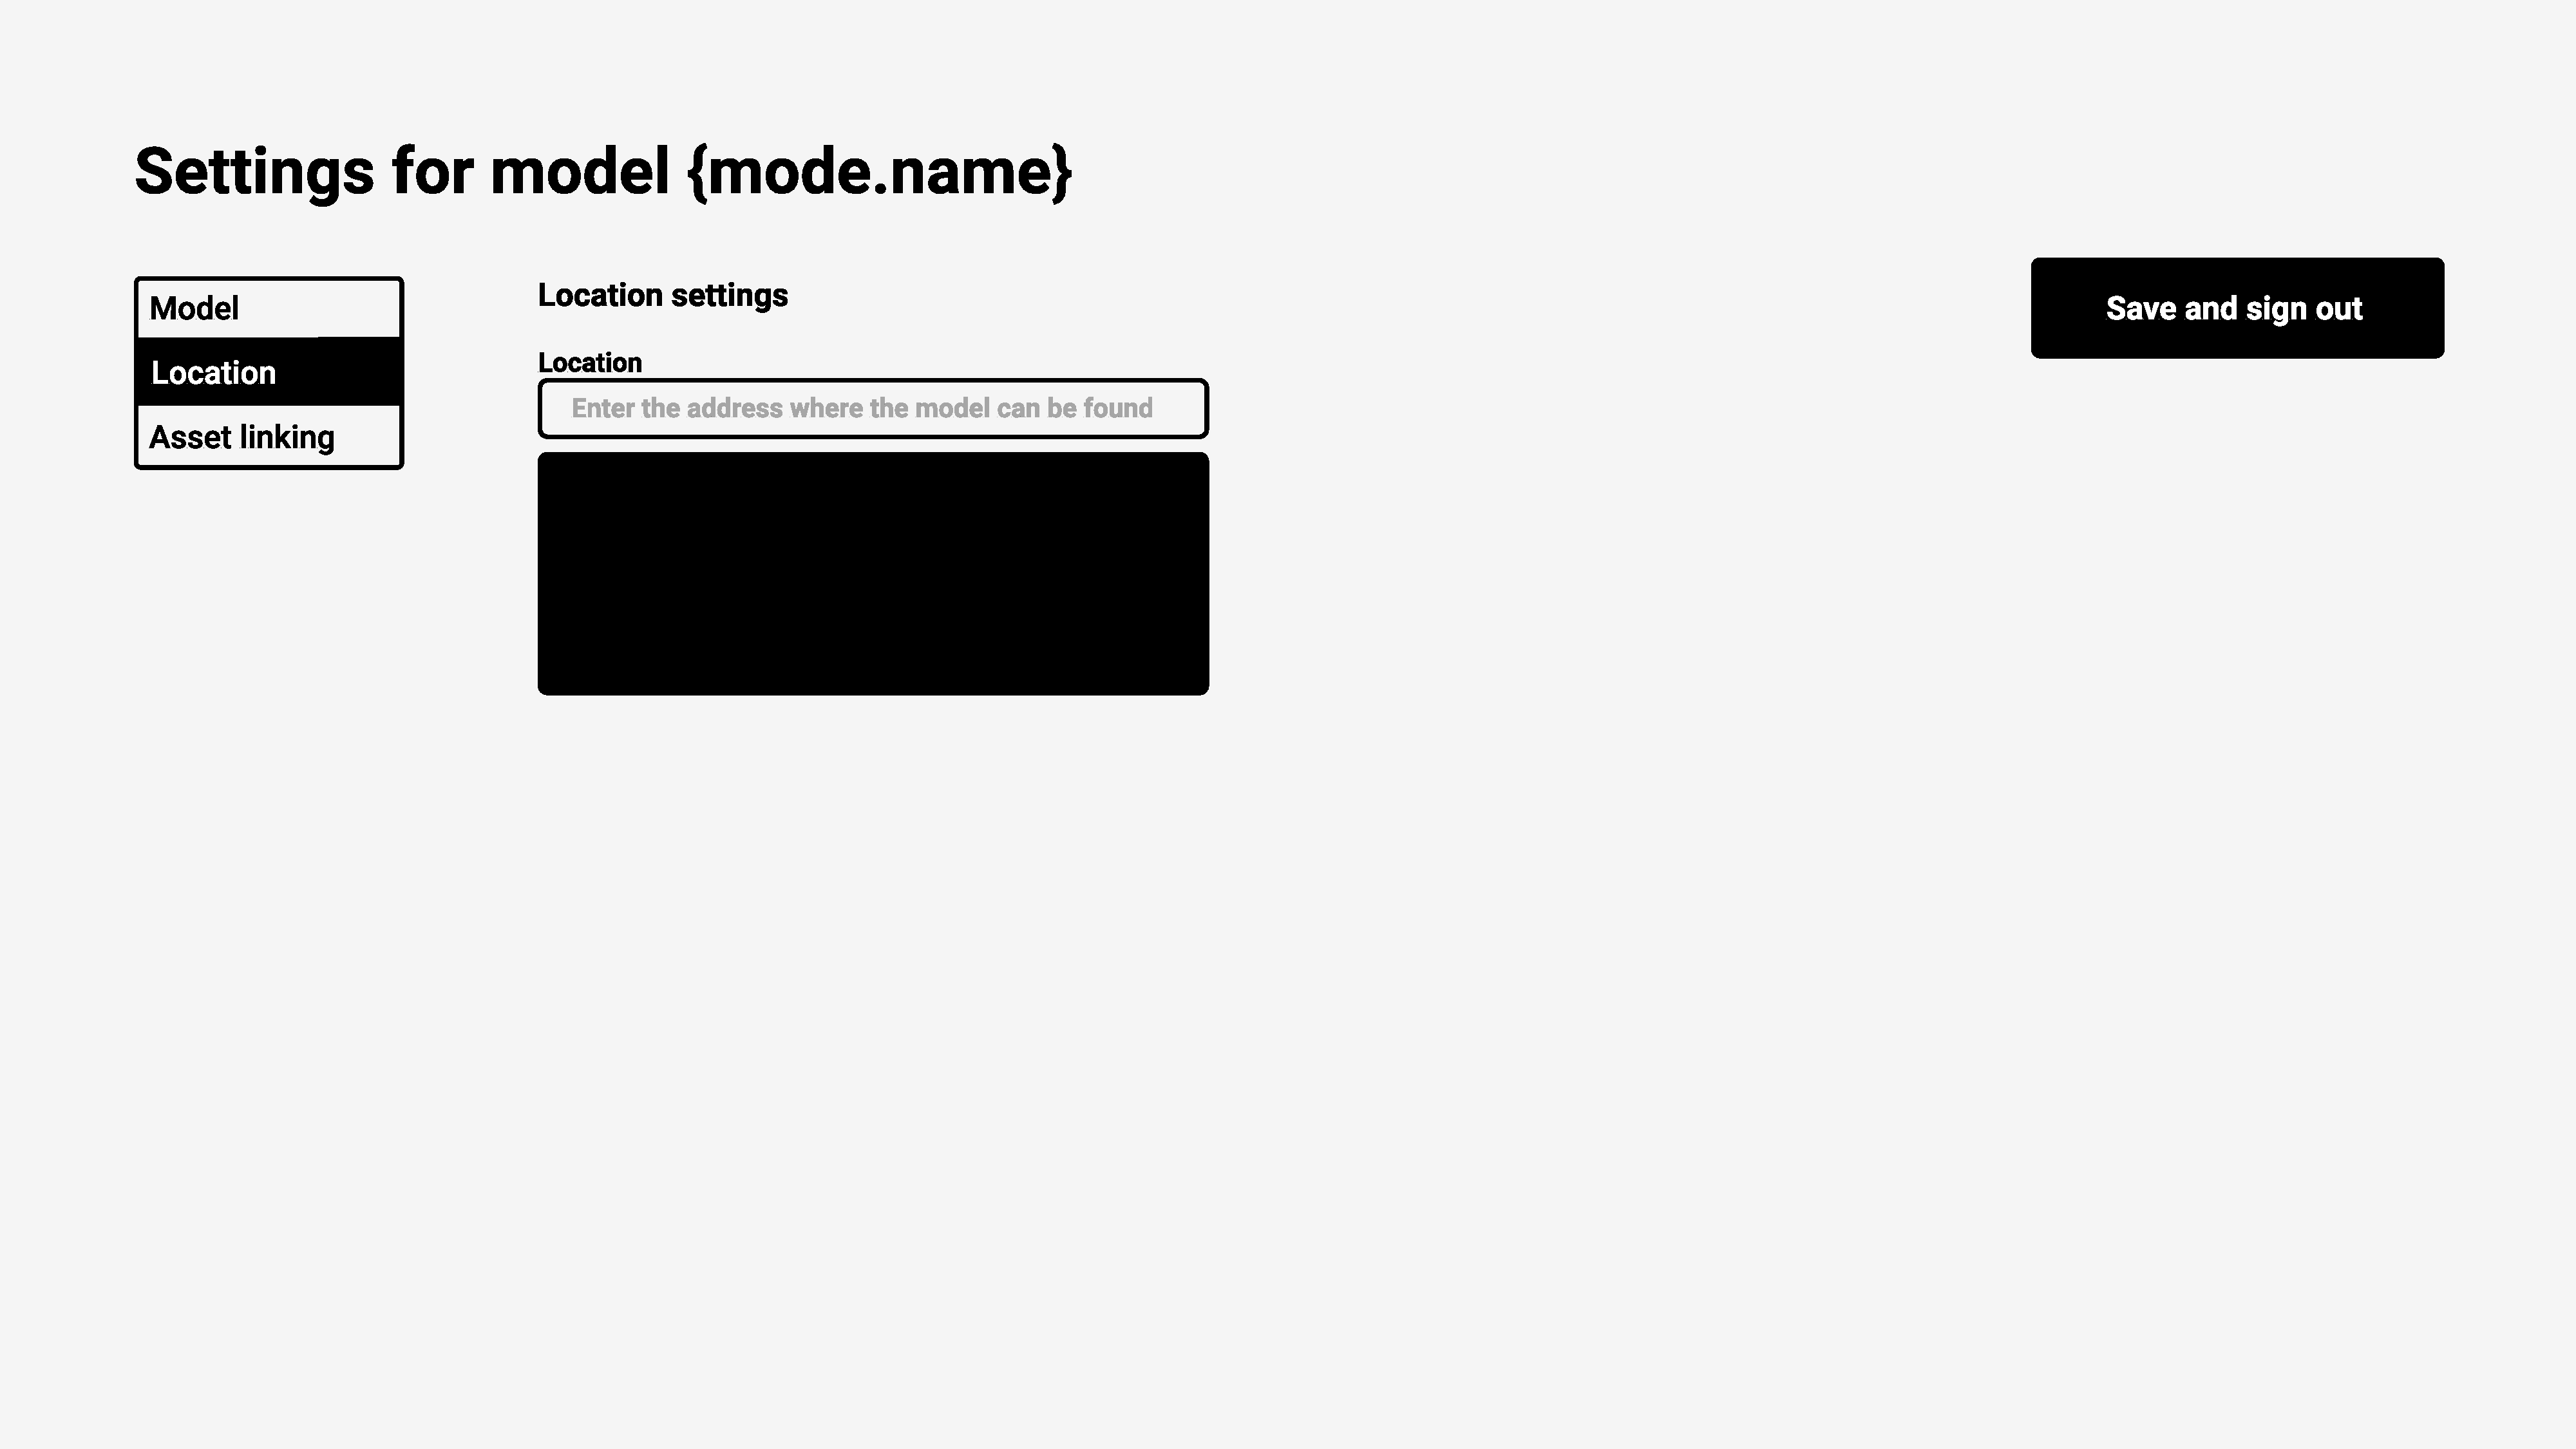
\includegraphics[width=1\textwidth]{./mockups/settings/Model-1.pdf}
  \caption[{Mockup des Standorteinstellungsmenü}]{Mockup des Standorteinstellungsmenü}
  \label{fig:mck-model_1}
\end{figure}
\pagebreak
\subsubsection{Verlinkungseinstellungen}
Nachfolgend ist ein Design für die Verlinkungseinstellungsseite. Hier kann der OSE Verantwortlicher Verlinkung des Modells ändern.
\begin{figure}[H]
  \centering
  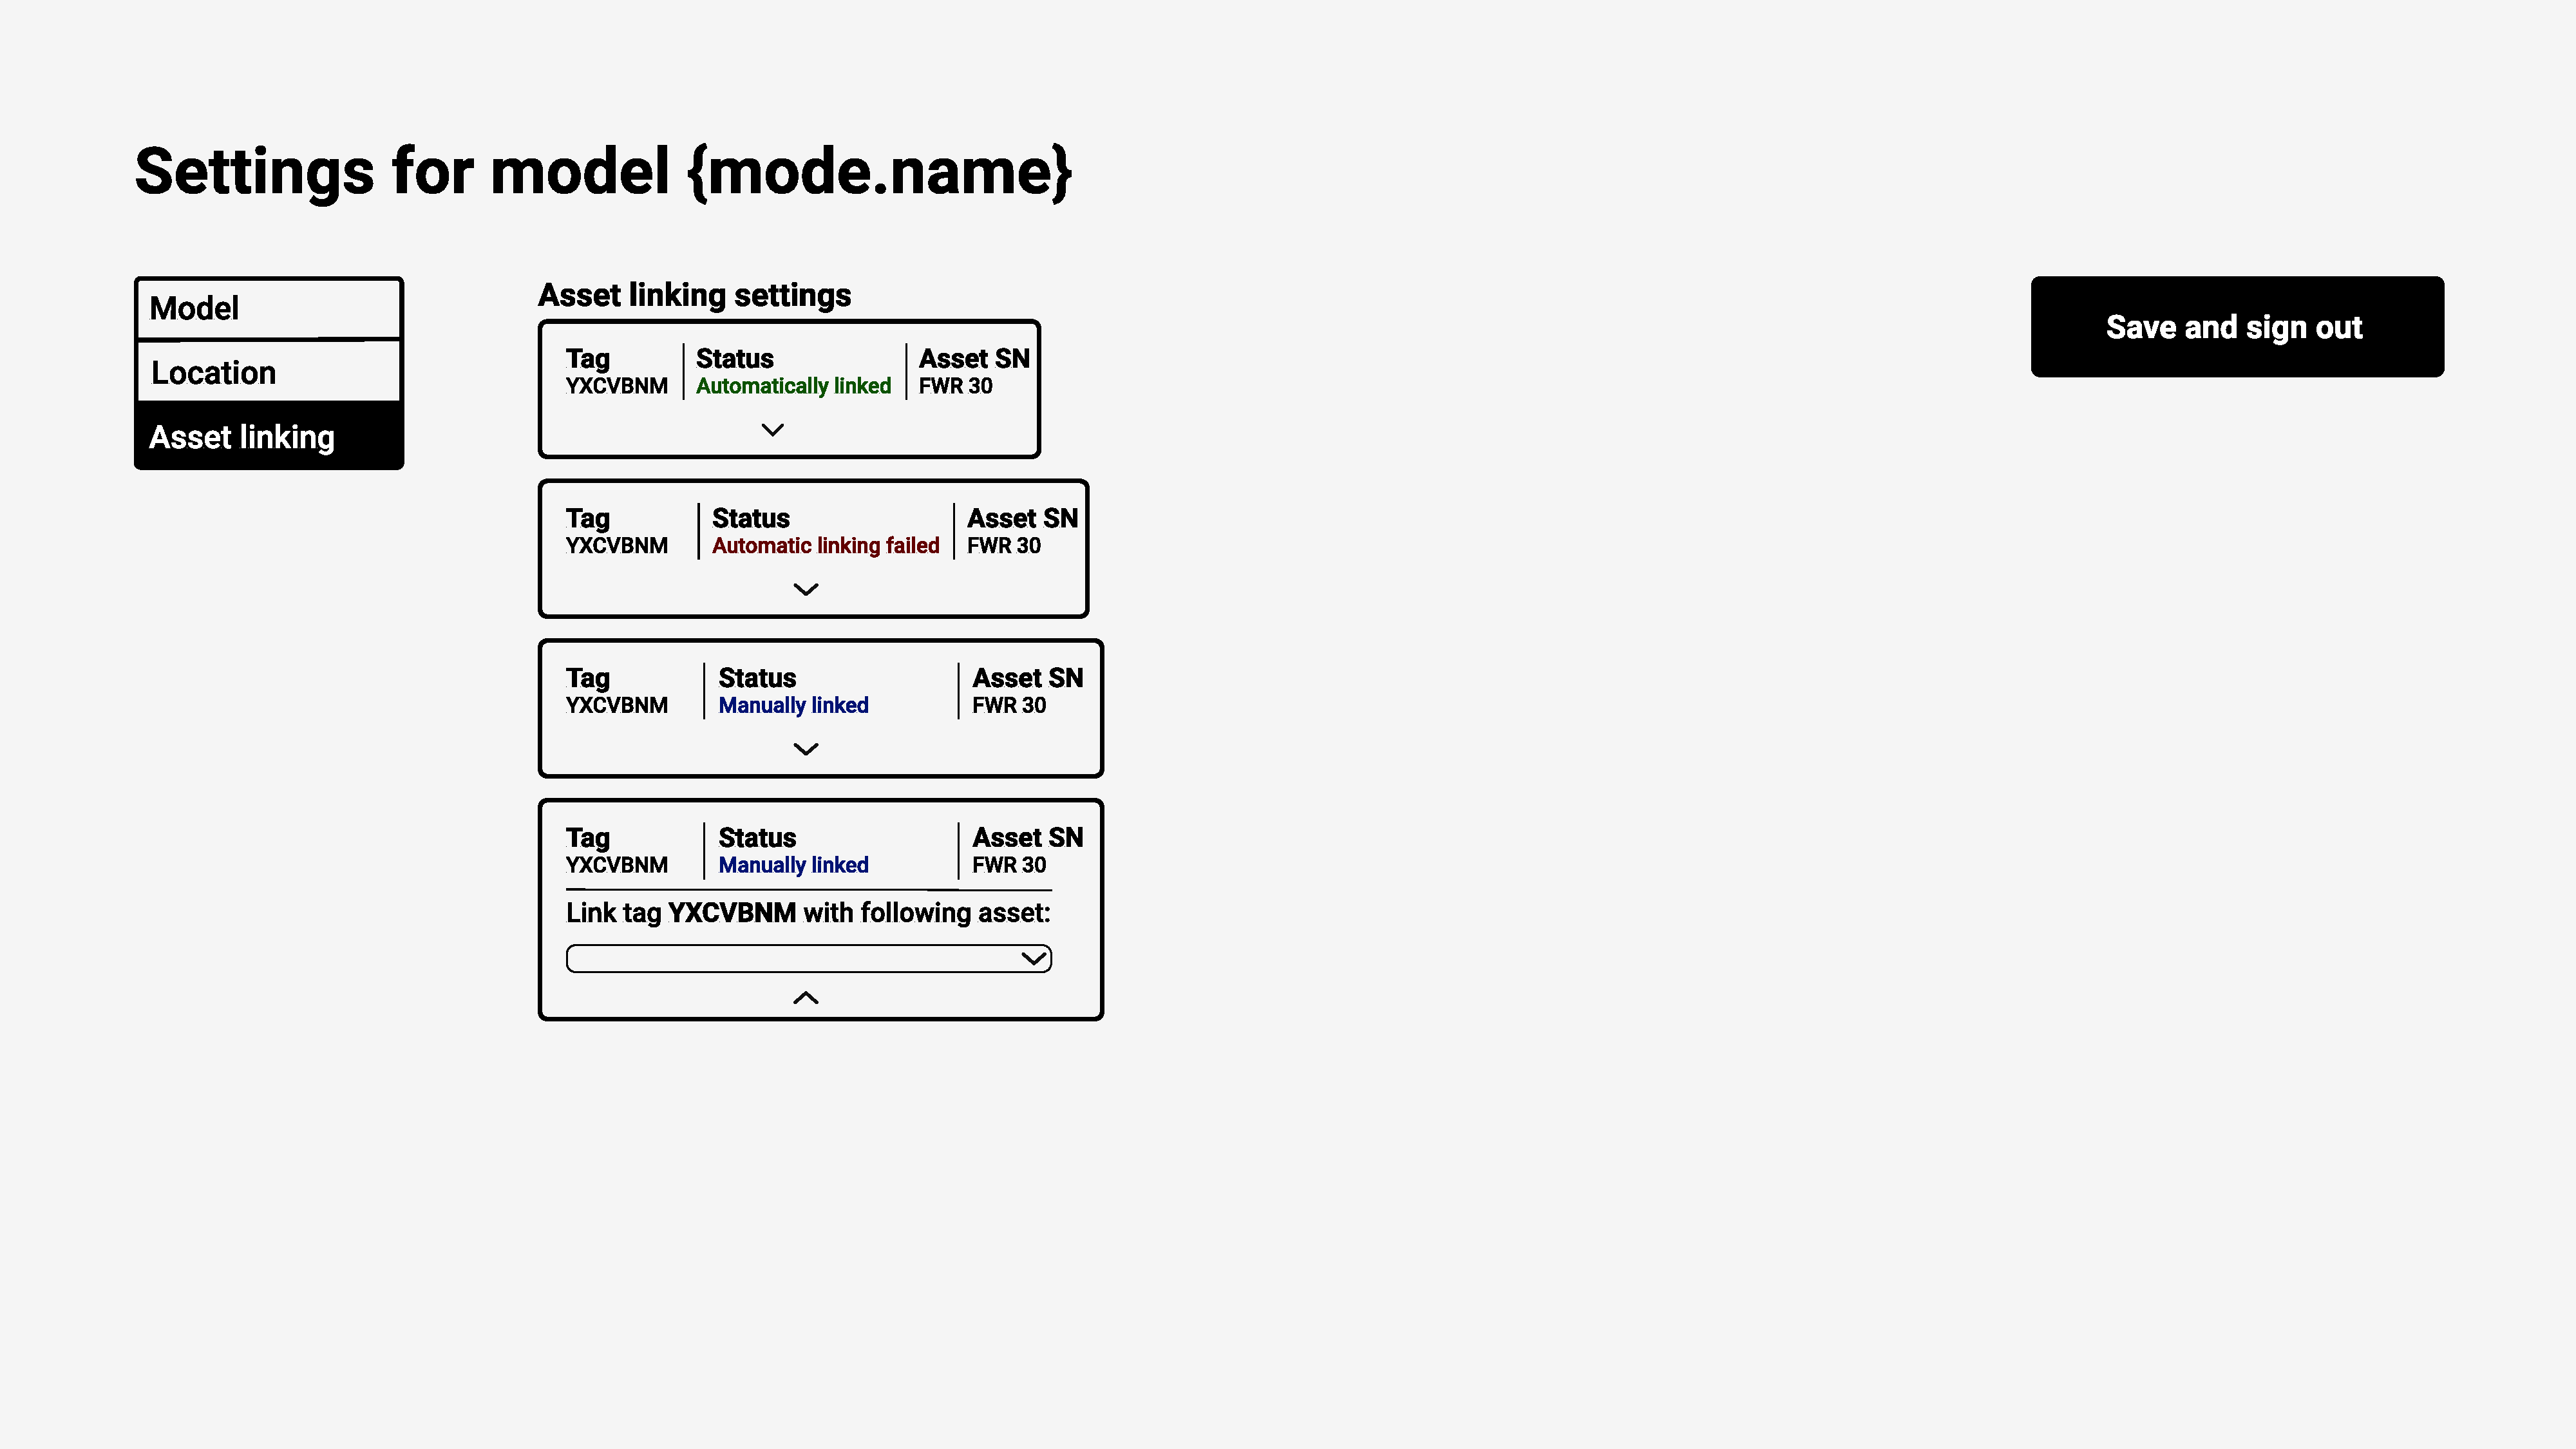
\includegraphics[width=1\textwidth]{./mockups/settings/Model-2.pdf}
  \caption[{Mockup des Verlinkungseinstellungsmenü}]{Mockup des Verlinkungseinstellungsmenü}
  \label{fig:mck-model_2}
\end{figure}
\section{Testkonzept}\label{testkonzept}
Damit sich bei der Abnahme des Projektes sicher gegangen werden kann, dass alles wie gewünscht funktioniert, wird ein Testkonzept erarbeitet. Dieses soll sich auf die bereits erstellten User-Stories stützen und so alle Anforderungen der Anspruchsgruppen abdecken. Nach der Implementierungsphase wird dieses Konzept befolgt und differenzen dokumentiert.
\newline
Einzelne Test-Cases werden wie folgt benannt:
\begin{table}[H]
  \begin{tabularx}{\textwidth}{l l X}\hline \\
  \textbf{Segment} & \textbf{Abkürzung} & \textbf{Beschreibung} \\ \\\hline \\
  1 & TC & Abkürzung für Test Case \\
  2 & - & Trennzeichen \\
  3 & 01 & Fortlaufende Kennzahl \\
  \\\hline
  \end{tabularx}
\end{table}
\subsection{Fehlerklassen}
Damit Testergebnisse nach der Prüfung priorisiert werden können, werden ihnen Fehlerklassen zugewiesen.
Fehlerklassen sind folgenderweise definiert:
\begin{table}[H]
  \begin{tabularx}{\textwidth}{l l X}\hline \\
  \textbf{Fehlerklasse} & \textbf{Beschreibung} \\ \\\hline \\
  0 & Definiertes Resultat stimmt mit dem getesteten Resultat überein \\
  1 & Definiertes Resultat weicht von dem getestet Resultat ab, beeinträchtigt die \\
    & Funktionalität allerdings nicht \\
  2 & Definiertes Resultat weicht von dem getestet Resultat ab und beeinträchtigt \\
    & die Funktionalität \\
  3 & Definiertes Resultat und getestetes Resultat stimmen nicht überein \\
  \\\hline
  \end{tabularx}
\end{table}
\subsection{Test Case Schema}
\begin{table}[H]
  \begin{tabularx}{\textwidth}{l l X}\hline \\
  \textbf{Segment} & \textbf{Beschreibung} \\ \\\hline \\
  Name & Name des Testes, gemäss des Namenskonzeptes \\
  Tester & Name der Person, die den Test durchgeführt hat \\
  Erwartetes Resultat & Vom Nutzer gewünschtes Resultat \\
  Effektives Resultat & Eingetroffenes Resultat \\
  Szenario & In Schritten definiertes Testszenario \\
  Fehlerklasse & Zugewiesene Fehlerklasse nach der Überprüfung \\
  Weiteres Vorgehen & Vorgehensbeschreibung, sollte die Fehlerklasse nicht 0 sein \\
  Status & Zeigt, ob der Test Case geprüft wurde \\
  \\\hline
  \end{tabularx}
\end{table}
\subsection{User-Stories Abdeckung}
\begin{table}[H]
  \begin{tabularx}{\textwidth}{l X l}\hline \\
  \textbf{Test-Case} & \textbf{Beschreibung} & \textbf{Betroffene User-Story} \\\hline \\
  TC-01 & Login möglich und sicher -> OAuth2konzept befolgt & US-01 \\
  TC-02 & Fehlermeldung Login & US-01 \\
  TC-03 & Automatische verlinkung Assets & US-02 \\
  TC-04 & Konfigurationsmenü aufrufbar & US-03 \\
  TC-05 & Verlinkungen manuel änderbar & US-03 \\
  TC-06 & Konfigurationsmenü nur durch eingeloggten User, welcher sich in der Usergruppe befindet, aufrufbar & US-04 \\
  TC-07 & Übersicht aller Standorte & US-06 \\
  TC-08 & Standort änderbar & US-06 \\
  \\\hline
  \end{tabularx}
\end{table}
\pagebreak
\subsection{Test-Cases}
\subsubsection{TC-01: Login}\label{tc-01}
\begin{table}[H]
  \begin{tabularx}{\textwidth}{l X}\hline \\
  Name & TC-01 \\
  Tester & Jonas Schultheiss \\
  Erwartetes Resultat & OSE Verantwortlicher kann sich anmelden \\
  Effektives Resultat & Das effektive Resultat stimmt mit dem erwarteten überein \\
  Fehlerklasse & 0 \\
  Weiteres Vorgehen & Nicht nötig \\
  Status & Durchgeführt am 13.04.2021 \\
  \\\hline
  \end{tabularx}
\end{table}
\begin{table}[H]
  \begin{tabularx}{\textwidth}{l X X}
  \textbf{Schritt} & \textbf{Beschreibung} & \textbf{Erwartetes Resultat}\\ \\\hline \\
  0 & Benutzer befindet sich auf der Startseite & / \\
  1 & Benutzer klickt den Knopf \amk{Sign in with Netilion} an & Client des Benutzers wird an Netilion ID weitergeleited \\
  2 & Benutzer gibt seine Daten an und loggt sich ein & Client des Benutzers wird zurück an das OSE-Dashboard geleited \\
  3 & Benutzer nicht registriert & Benutzer wird zur Registration weitergeleited \\
  Alternative & Benutzer registriert & Benutzer wird zum Konfigurationsmenü weitergeleited \\
  \\\hline
  \end{tabularx}
\end{table}
\pagebreak
\subsubsection{TC-02: Login falsche Logindaten}\label{tc-02}
\begin{table}[H]
  \begin{tabularx}{\textwidth}{l X}\hline \\
  Name & TC-02 \\
  Tester & Jonas Schultheiss \\
  Erwartetes Resultat & Anmeldeprozess läuft schief, aber wird bei Netilion ID direkt behandelt \\
  Effektives Resultat & Das effektive Resultat stimmt mit dem erwarteten überein \\
  Fehlerklasse & 0 \\
  Weiteres Vorgehen & Nicht nötig \\
  Status & Durchgeführt am 13.04.2021 \\
  \\\hline
  \end{tabularx}
\end{table}
\begin{table}[H]
  \begin{tabularx}{\textwidth}{l X X}
  \textbf{Schritt} & \textbf{Beschreibung} & \textbf{Erwartetes Resultat}\\ \\\hline \\
  0 & Benutzer befindet sich auf der Startseite & / \\
  1 & Benutzer klickt den Knopf \amk{Sign in with Netilion} an & Client des Benutzers wird an Netilion ID weitergeleited \\
  2 & Benutzer gibt seine Daten an und probiert sich anzumelden & Netilion ID zeigt Fehlermeldung an \\
  \\\hline
  \end{tabularx}
\end{table}
\pagebreak
\subsubsection{TC-03: Login mit unberechtigtem Account}\label{tc-03}
\begin{table}[H]
  \begin{tabularx}{\textwidth}{l X}\hline \\
  Name & TC-03 \\
  Tester & Jonas Schultheiss \\
  Erwartetes Resultat & Anmeldeprozess funktioniert und Bentzer erhält passende Fehlermeldung \\
  Effektives Resultat & Das effektive Resultat stimmt mit dem erwarteten überein \\
  Fehlerklasse & 0 \\
  Weiteres Vorgehen & Nicht nötig \\
  Status & Durchgeführt am 13.04.2021 \\
  \\\hline
  \end{tabularx}
\end{table}
\begin{table}[H]
  \begin{tabularx}{\textwidth}{l X X}
  \textbf{Schritt} & \textbf{Beschreibung} & \textbf{Erwartetes Resultat}\\ \\\hline \\
  0 & Benutzer befindet sich auf der Startseite & / \\
  1 & Benutzer klickt den Knopf \amk{Sign in with Netilion} an & Client des Benutzers wird an Netilion ID weitergeleited \\
  2 & Benutzer gibt seine Daten an und meldet sich an & Client des Benutzers wird zurück an das OSE-Dashboard geleited, wo eine passende Fehlermeldung angezeigt wird \\
  \\\hline
  \end{tabularx}
\end{table}
\pagebreak
\subsubsection{TC-04: Automatische Verlinkung der Assets}\label{tc-04}
\begin{table}[H]
  \begin{tabularx}{\textwidth}{l X}\hline \\
  Name & TC-04 \\
  Tester & Jonas Schultheiss \\
  Erwartetes Resultat & Assets und Meshes werden automatisch verlinkt \\
  Effektives Resultat & Kann ein Asset nicht mit einem Mesh verlinkt werden, bekommt dies der Nutzer nicht mit \\
  Fehlerklasse & 1 \\
  Weiteres Vorgehen & Wird in Kapitel \ref{abschluss} beschrieben \\
  Status & Durchgeführt am 13.04.2021 \\
  \\\hline
  \end{tabularx}
\end{table}
\begin{table}[H]
  \begin{tabularx}{\textwidth}{l X X}
  \textbf{Schritt} & \textbf{Beschreibung} & \textbf{Erwartetes Resultat}\\ \\\hline \\
  0 & Noch nicht registrierter Benutzer hat sich bereits angemeldet und befindet sich auf dem zweiten Tab der Registration & / \\
  1 & Benutzer geht zum nächsten Tab & Client zeigt an, dass die Verlinkung im Gange ist und Backend verlinkt die Entitäten \\
  2A & Alle Assets verlinkt & Benutzer wird benachrichtigt und kann sich ausloggen \\
  Alternative & Nicht alle Assets verlinkt & Benutzer wird benachrichtigt und kann zum Konfigurationsmenü fortfahren \\
  \\\hline
  \end{tabularx}
\end{table}
\pagebreak
\subsubsection{TC-05: Konfigurationsmenü aufrufbar}\label{tc-05}
\begin{table}[H]
  \begin{tabularx}{\textwidth}{l X}\hline \\
  Name & TC-05 \\
  Tester & Jonas Schultheiss \\
  Erwartetes Resultat & Konfigurationsmenü ist aufrufbar \\
  Effektives Resultat & Das effektive Resultat stimmt mit dem erwarteten überein \\
  Fehlerklasse & 0 \\
  Weiteres Vorgehen & Nicht nötig \\
  Status & Durchgeführt am 13.04.2021 \\
  \\\hline
  \end{tabularx}
\end{table}
\begin{table}[H]
  \begin{tabularx}{\textwidth}{l X X}
  \textbf{Schritt} & \textbf{Beschreibung} & \textbf{Erwartetes Resultat}\\ \\\hline \\
  0 & Bereits registrierter Benutzer befindet sich auf der Startseite  & / \\
  1 & Benutzer meldet sich an & Client wird zum Konfigurationsmenü weitergeleited \\
  \\\hline
  \end{tabularx}
\end{table}
\begin{table}[H]
  \begin{tabularx}{\textwidth}{l X X}
  \textbf{Schritt} & \textbf{Beschreibung} & \textbf{Erwartetes Resultat}\\ \\\hline \\
  0 & Noch nicht registrierter Benutzer befindet sich auf der Startseite  & / \\
  1 & Benutzer meldet sich an & Client wird zur Registration weitergeleited \\
  2 & Benutzer registriert sich & Client wird zum Konfigurationsmenü weitergeleited \\
  \\\hline
  \end{tabularx}
\end{table}
\pagebreak
\subsubsection{TC-06: Verlinkung manuell änderbar}\label{tc-06}
\begin{table}[H]
  \begin{tabularx}{\textwidth}{l X}\hline \\
  Name & TC-06 \\
  Tester & Jonas Schultheiss \\
  Erwartetes Resultat & Assets und Meshes werden manuell verlinkt \\
  Effektives Resultat & Das effektive Resultat stimmt mit dem erwarteten überein \\
  Fehlerklasse & 0 \\
  Weiteres Vorgehen & Nicht nötig \\
  Status & Durchgeführt am 13.04.2021 \\
  \\\hline
  \end{tabularx}
\end{table}
\begin{table}[H]
  \begin{tabularx}{\textwidth}{l X X}
  \textbf{Schritt} & \textbf{Beschreibung} & \textbf{Erwartetes Resultat}\\ \\\hline \\
  0 & Bereits registrierter Benutzer befindet sich im Konfigurationsmenü im Assets Tab  & / \\
  1 & Benutzer klickt auf eine Verlinkung & Verlinkungkomponente öffnet sich \\
  2 & Benutzer klickt auf das Dropdown & Dropdown öffnet und stellt alle verfügbaren Assets dar \\
  3 & Benutzer selektiert anderen Mesh & Knopf \amk{Save changes} wird freigeschaltet \\
  4 & Benutzer klickt Knopf & Änderungen werden gespeichert \\
  \\\hline
  \end{tabularx}
\end{table}
\pagebreak
\subsubsection{TC-07: Übersicht aller Standorte}\label{tc-07}
\begin{table}[H]
  \begin{tabularx}{\textwidth}{l X}\hline \\
  Name & TC-07 \\
  Tester & Jonas Schultheiss \\
  Erwartetes Resultat & Benutzer sieht übersicht aller Standorte \\
  Effektives Resultat & Das effektive Resultat stimmt mit dem erwarteten überein \\
  Fehlerklasse & 0 \\
  Weiteres Vorgehen & Nicht nötig \\
  Status & Durchgeführt am 13.04.2021 \\
  \\\hline
  \end{tabularx}
\end{table}
\begin{table}[H]
  \begin{tabularx}{\textwidth}{l X X}
  \textbf{Schritt} & \textbf{Beschreibung} & \textbf{Erwartetes Resultat}\\ \\\hline \\
  0 & Benutzer befindet sich auf der Startseite  & / \\
  1 & Benutzer öffnet die Augen & Benutzer sieht auf der initialen Ansicht der Startseite die Standortauswahl \\
  \\\hline
  \end{tabularx}
\end{table}
\pagebreak
\subsubsection{TC-08: Standort änderbar}\label{tc-08}
\begin{table}[H]
  \begin{tabularx}{\textwidth}{l X}\hline \\
  Name & TC-08 \\
  Tester & Jonas Schultheiss \\
  Erwartetes Resultat & Standort ist änderbar \\
  Effektives Resultat & Das effektive Resultat stimmt mit dem erwarteten überein \\
  Fehlerklasse & 0 \\
  Weiteres Vorgehen & Nicht nötig \\
  Status & Durchgeführt am 13.04.2021 \\
  \\\hline
  \end{tabularx}
\end{table}
\begin{table}[H]
  \begin{tabularx}{\textwidth}{l X X}
  \textbf{Schritt} & \textbf{Beschreibung} & \textbf{Erwartetes Resultat}\\ \\\hline \\
  0 & Bereits registrierter Benutzer befindet sich auf der Startseite  & / \\
  1 & Benutzer meldet sich an & Benutzer wird angemeldet und zum Konfigurationsmenü weitergeleitet \\
  2 & Benutzer klickt auf den Tab \amk{Location} & Benutzer wird zu \code{/settings/location} weitergeleitet \\
  3 & Benutzer gibt im Eingabefeld eine neue Addresse ein & Passende Adressen wird automatisch werden vorgeschlagen \\
  4 & Benutzer klickt auf einen Adressensvorschlag & Adresse wird im Eingabefeld vervollständigt \\
  5 & Benutzer klickt auf den Knopf \amk{Save changes} & Änderungen werden gespeichert \\
  \\\hline
  \end{tabularx}
\end{table}
\pagebreak
\section{Datenbankerweiterung}
Damit die gewünschten Änderungen implementiert werden können, muss die Datenbank erweitert werden. Die Änderungen sind in der Abbildung \ref{fig:db-erweiterung} grün dargestellt. Grau markierte Tabellen sind bereits bestehende Elemente, welche in der Vorarbeit implementiert wurden.
\begin{figure}[H]
  \centering
  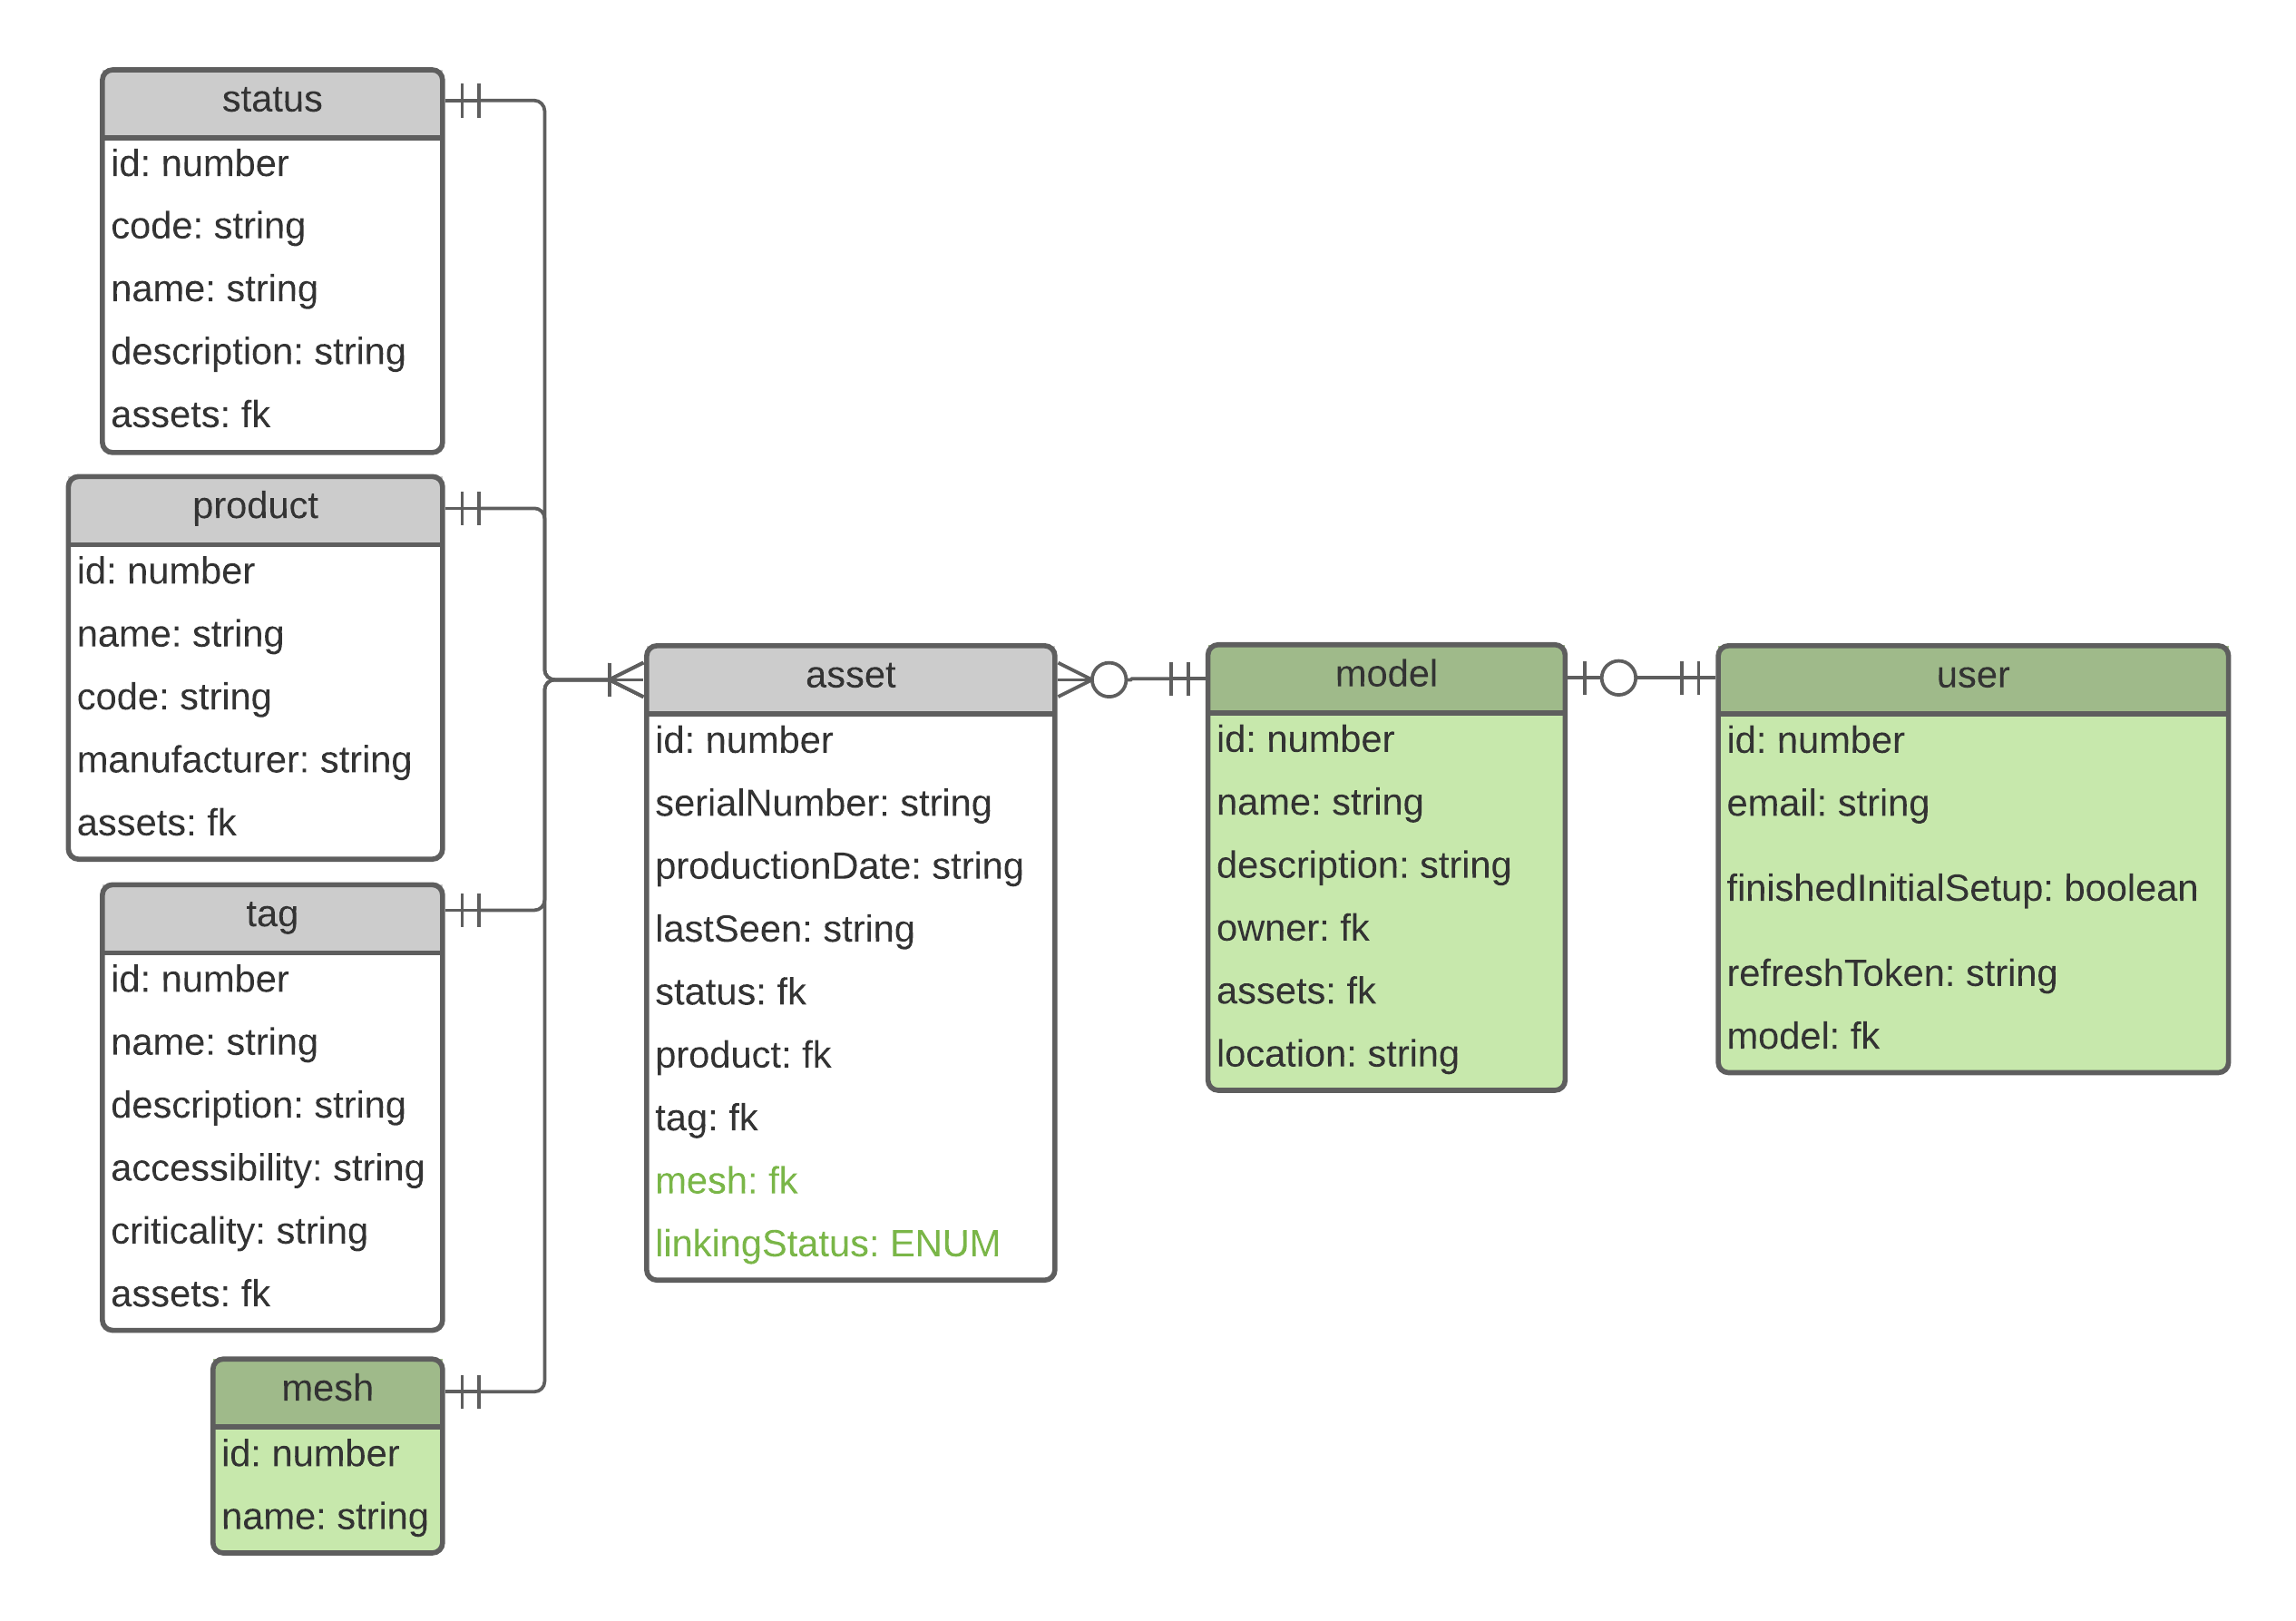
\includegraphics[width=.95\linewidth]{./images/ERM-OSE.png}
  \caption[{ERM welches die Datenbankerweiterung visualisiert}]{ERM welches die Datenbankerweiterung visualisiert}
  \label{fig:db-erweiterung}
\end{figure}
\subsection{User}
Die Userentität hat drei verwendungen:
\begin{itemize}
  \item Soll zu einem JWT geformt werden, welcher zur authentifizierung verwendet werden soll
  \item Soll den \code{refresh\_token} speichern
  \item Soll speichern, ob der User die Registration abgeschlossen hat
\end{itemize}
\subsection{Model}
Das Modell soll einen Namen und eine Beschreibung enthalten. Diese Angaben können später verwendet werden, wenn das jeweilige Modell angezeigt wird. Das Attribut \amk{location} enthält eine Id, mit welcher die genaue Adresse und Koordinaten beim Backend angefragt werden können. Ausserdem dient das Modell als Bindeglied zwischen dem \amk{User} und den \amk{Assets}.
\subsection{Mesh}
Das Mesh wird wird verwendet um die Verlinkung zwischen dem 3D-Modell und dem einzelnen Asset zu ermöglichen. Das Mesh selbst enthält dabei nur einen Namen. Bei der Planung dieser IPA wurde nicht beachtet, dass die Namen der Meshes hinzugefügt werden müssen. Da es keinen Administrator in der Applikation gibt und Nestjs, beziehungsweise das darunterliegende ORM TypeOrm, kein Seeding unterstützt, müssen diese Daten manuel der Datenbank hinzugefügt werden. Im Repository des Backends soll ein SQL und ein CSV hinterlegt werden, womit die Daten dann mit Postico, einem PostgreSQL Client, hinzugefügt werden können.
\newline
Damit das Frontend auch anzeigen kann, ob ein Asset nun automatisch oder manuell verlinkt wurde, soll der Assetentität ein enum mit dem Namen \amk{linkingStatus} hinzugefügt werden. Dieses enum soll folgende Auswahl zur verfügung stellen:
\begin{itemize}
  \item Nicht verlinkt
  \item Automatisch verlinkt
  \item Automatische Verlinkung schlug fehl
  \item Manuell verlinkt
\end{itemize}
\section{Authentifizierung mit JWT}
Die Authentifizierung zwischen dem Front- und Backend, wird mit \amk{JSON Web Tokens} gelöst. Dies wurde vom Kandidaten in einigen vorherigen Arbeiten so angewendet und ist für Ihn der Standard, wenn die Schichten getrennt werden.
\subsection{Was ist ein JWT}
\amk{JSON Web Token (JWT) ist ein offener Standard (RFC 7519), der eine kompakte und in sich geschlossene Methode zur sicheren Übertragung von Informationen zwischen Parteien als JSON-Objekt definiert. Diese Informationen können verifiziert und vertrauenswürdig sein, da sie digital signiert sind. JWTs können mit einem Geheimnis (mit dem HMAC-Algorithmus) oder einem öffentlichen/privaten Schlüsselpaar mit RSA oder ECDSA signiert werden.
\newline
Obwohl JWTs auch verschlüsselt werden können, um die Geheimhaltung zwischen den Parteien zu gewährleisten, werden wir uns auf signierte Token konzentrieren. Signierte Token können die Integrität der darin enthaltenen Ansprüche verifizieren, während verschlüsselte Token diese Ansprüche vor anderen Parteien verbergen. Wenn Token mit öffentlichen/privaten Schlüsselpaaren signiert werden, bescheinigt die Signatur auch, dass nur die Partei, die den privaten Schlüssel besitzt, diejenige ist, die sie signiert hat.}\cite{auth0.com}.
\newline
\newline
Ein JWT besteht aus drei Bestandteilen: dem Header, der Payload und der Signatur. Der Header enthält den Algorithmus mit dem der JWT encoded wird und den Typ des Tokens. Der Payload kann von der Applikation selbst bestimmt werden, sollte allerdings klein gehalten werden, da der JWT bei jeder Anfrage im Header als \amk{Authorization} mitgesendet wird. Laut dem Standard müssen die Attribute \amk{sub} und \amk{iat} enthalten sein. Sie sagen nämlich aus, wer das Subjekt ist und wann der JWT ausgestellt wurde. Der letzte Teil des Tokens ist die Signatur, womit der Aussteller des Tokens die Integrität überprüfen kann.
\begin{figure}[H]
  \centering
  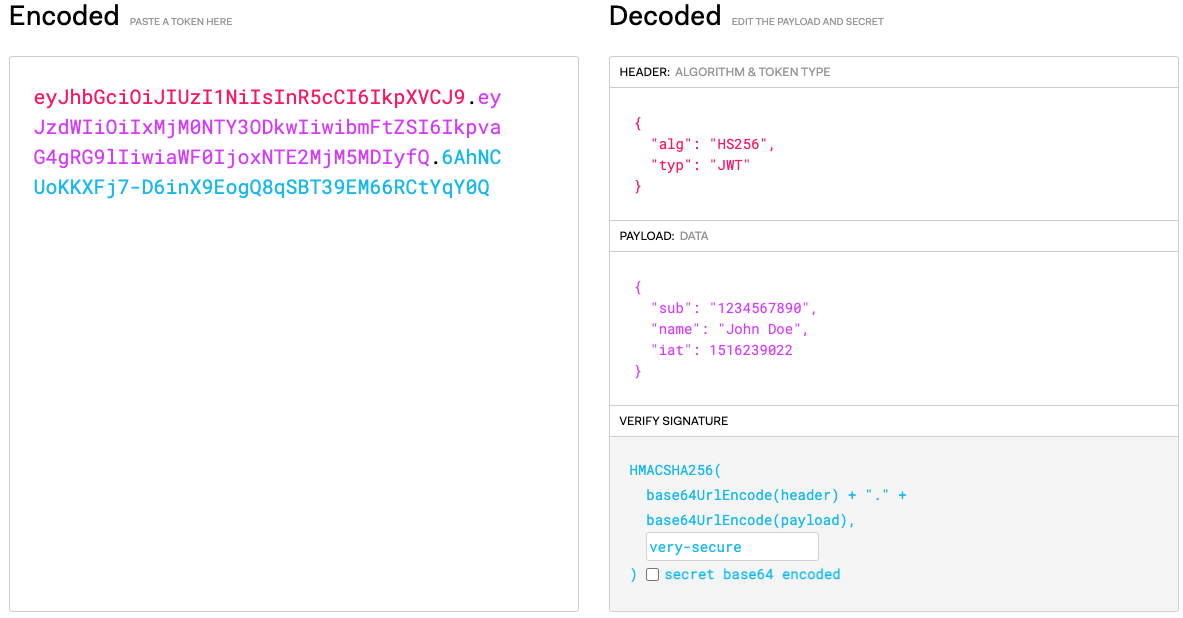
\includegraphics[width=.95\linewidth]{./images/jwt.io.png}
  \caption[{Screenshot von JWT.io}]{Screenshot von JWT.io}
  \label{fig:jwt}
\end{figure}
\subsection{Anwendung} \label{andwendung-jwt}
Bei einer erfolgreichen Anmeldung erstellt das Backend einen JWT. Dessen Inhalt ist die Id des Nutzers, die Email, ein Boolean womit das Frontend weiss, ob der User bereits ein Modell registriert hat, das Erstellungsdatum und das Verfallsdatum. Dieser wird an das Frontend zurückgegeben. Das Frontend speichert diesen im SessionStorage und sendet ihn bei jeder weiteren Anfrage mit. Somit weiss das Backend immer, wer die Anfrage erstellt hat.
\newline
Sollte zum Beispiel die Id des Nutzers im  JWT verändert werden, stimmt die Signatur nicht mehr und das Backend lehnt die Anfrage mit dem HTTP Status Code 401 ab.

\chapter{Implementierung}
\section{OAuth2}
\subsection{Frontend}
\begin{figure}[H]
  \centering
  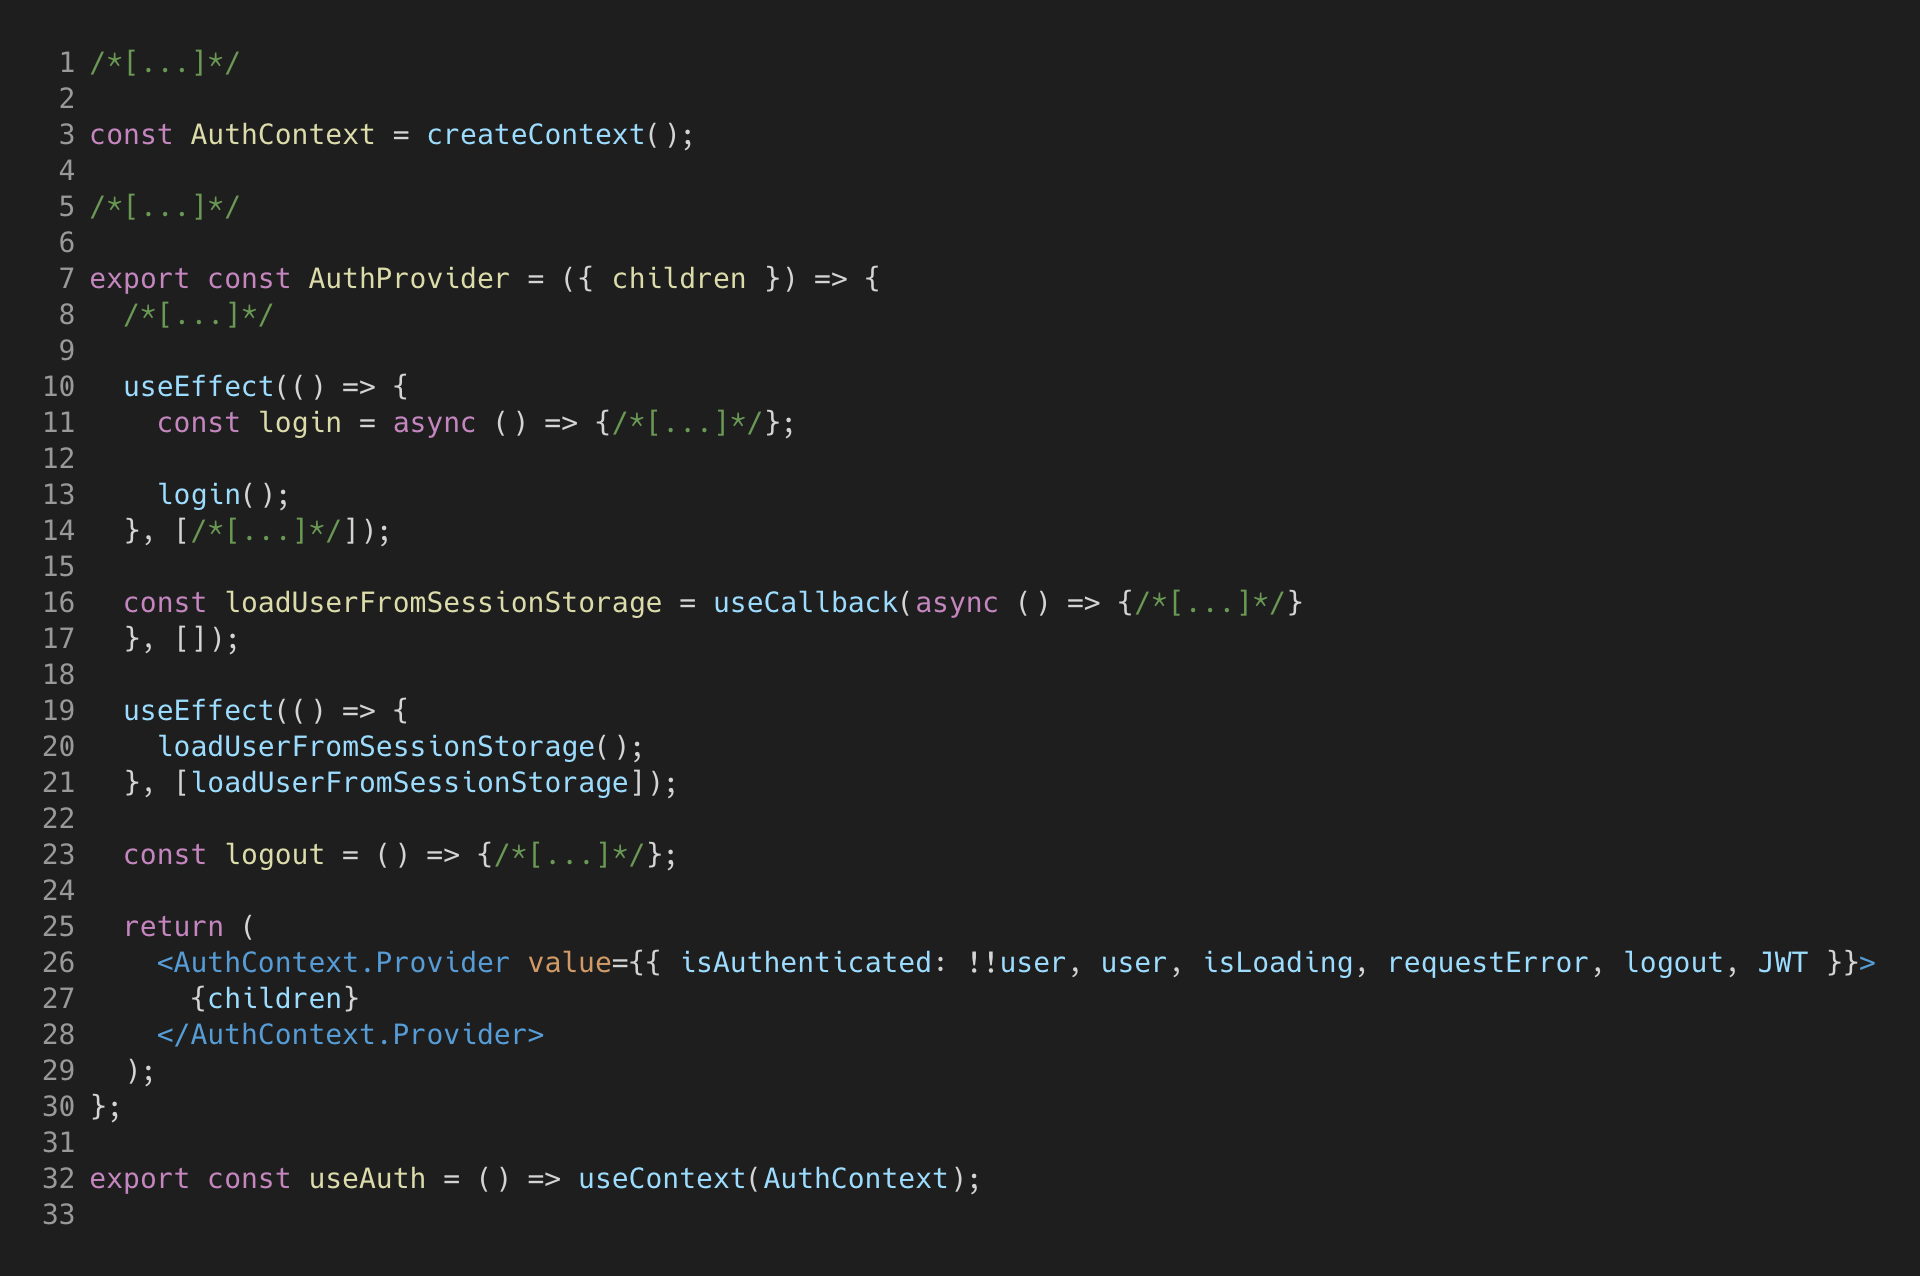
\includegraphics[width=.95\linewidth]{./images/authContext.png}
  \caption[{authContext.js von \code{ose-dashboard-frntnd}}]{authContext.js von \code{ose-dashboard-frntnd}}
  \label{fig:authContext}
\end{figure}
Dinge wie der JWT, Nutzerinformationen oder Funktionen wie \amk{login} und \amk{logout} müssen global in der Nextjs Applikation zur verfügung stehen. Vor ein paar Jahren hätte man dies noch mit Redux lösen müssen. Mittlerweile gibt es allerdings in React ein Konzept mit dem Namen \amk{Context}. Context erlaubt es einem, einen Wrapper mit State und Funktionen zu schreiben und diese den Subkomponenten zur verfügung zustellen. Werden Nutzerinformationen oder dazugehörige Funktionen in einer Subkomponente verwendet, können diese mit der \code{useAuth} Hook konsumiert werden. Dies sieht wie folgt aus:
\begin{figure}[H]
  \centering
  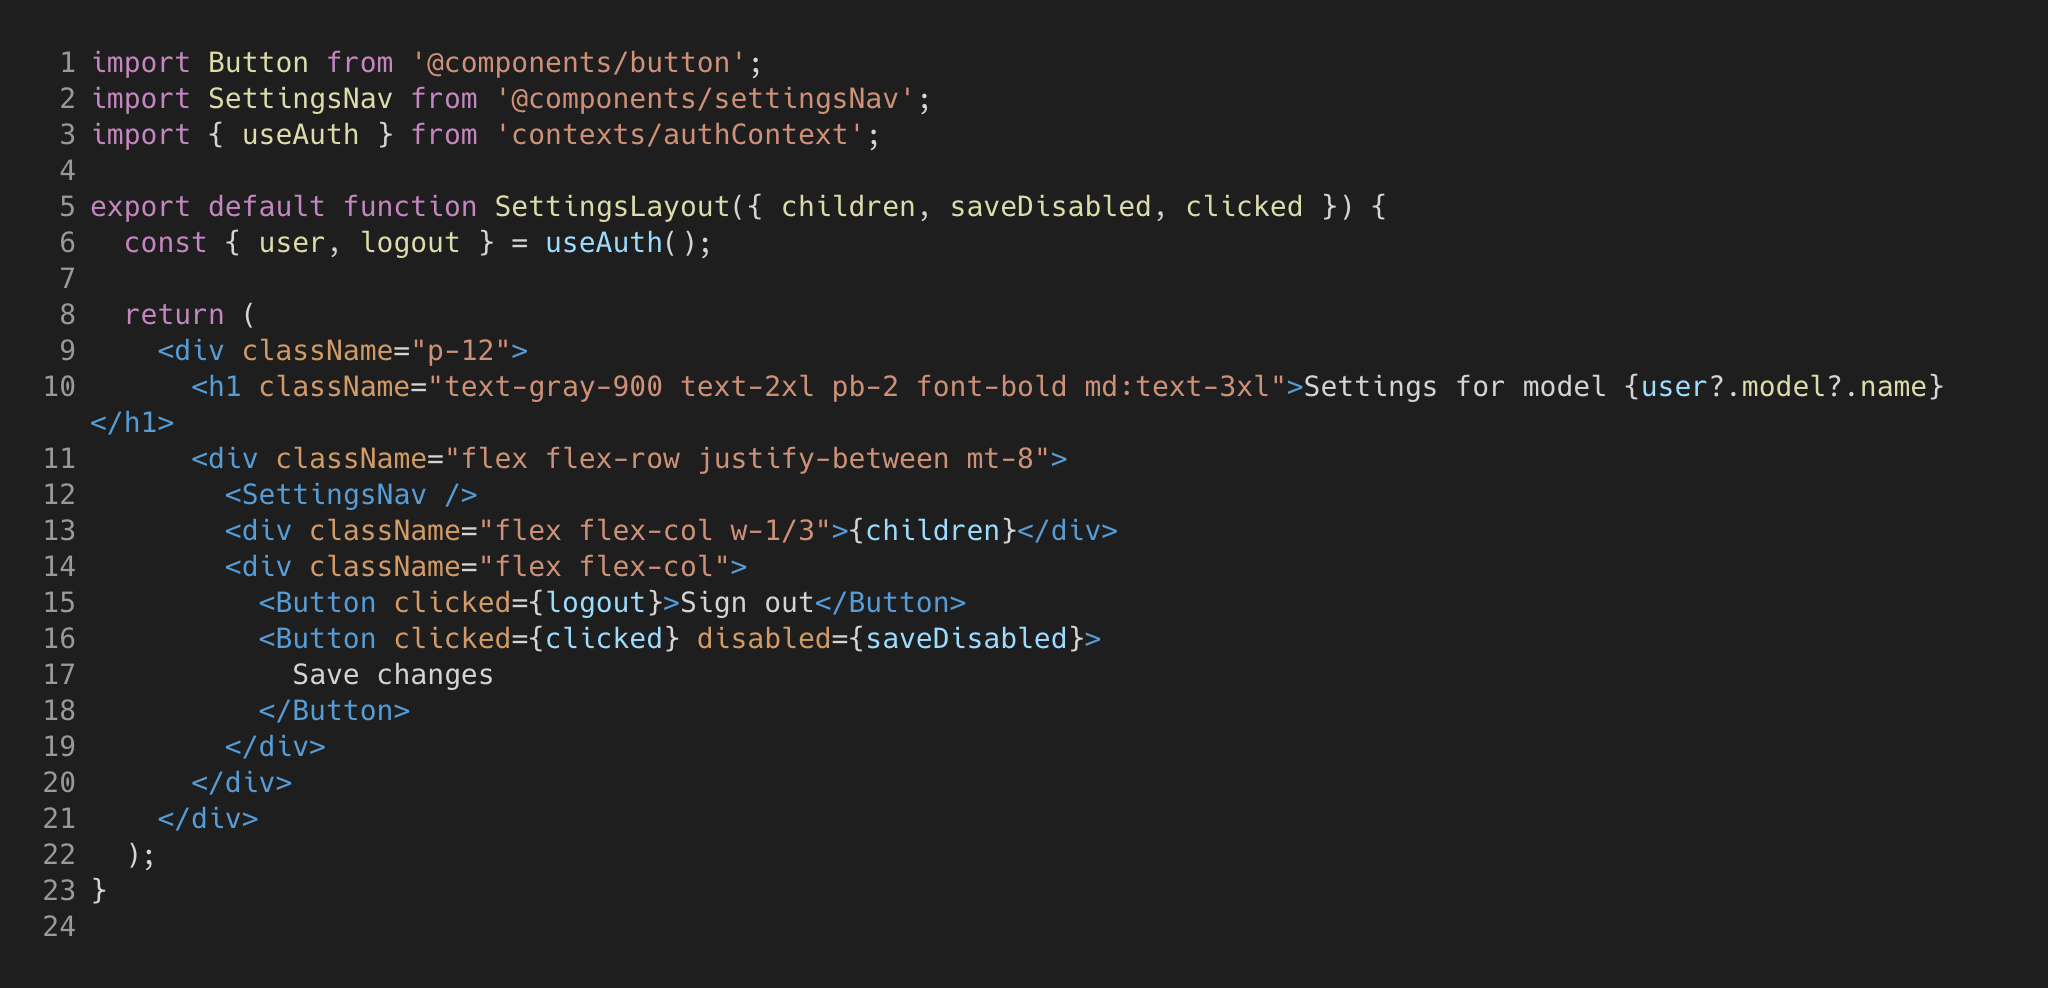
\includegraphics[width=.95\linewidth]{./images/settingsLayout.js.png}
  \caption[{settingsLayout.js von \code{ose-dashboard-frntnd}}]{settingsLayout.js von \code{ose-dashboard-frntnd}}
  \label{fig:settingsLayout}
\end{figure}
In der Zeile 6 wird der \amk{user} und die \amk{logout} Funktion vom Context konsumiert. Dies ermöglicht das anzeigen des Namen des Modelles auf Zeile 10 und das abmelden auf Zeile 15.
\subsection{Backend}
Der schwierige Teil der Implementierung von OAuth2 befindet sich allerdings im Backend. Eine Bedingung ist, dass sich der Nutzer anmelden kann. Die Zweite ist, dass alle Modelle in einem Intervall die Daten ihrer Assets aktualisieren. Diese Funktionalitäten sind in den beiden nachfolgenden Kapiteln beschrieben.
\subsubsection{Log-in}
\begin{figure}[H]
  \centering
  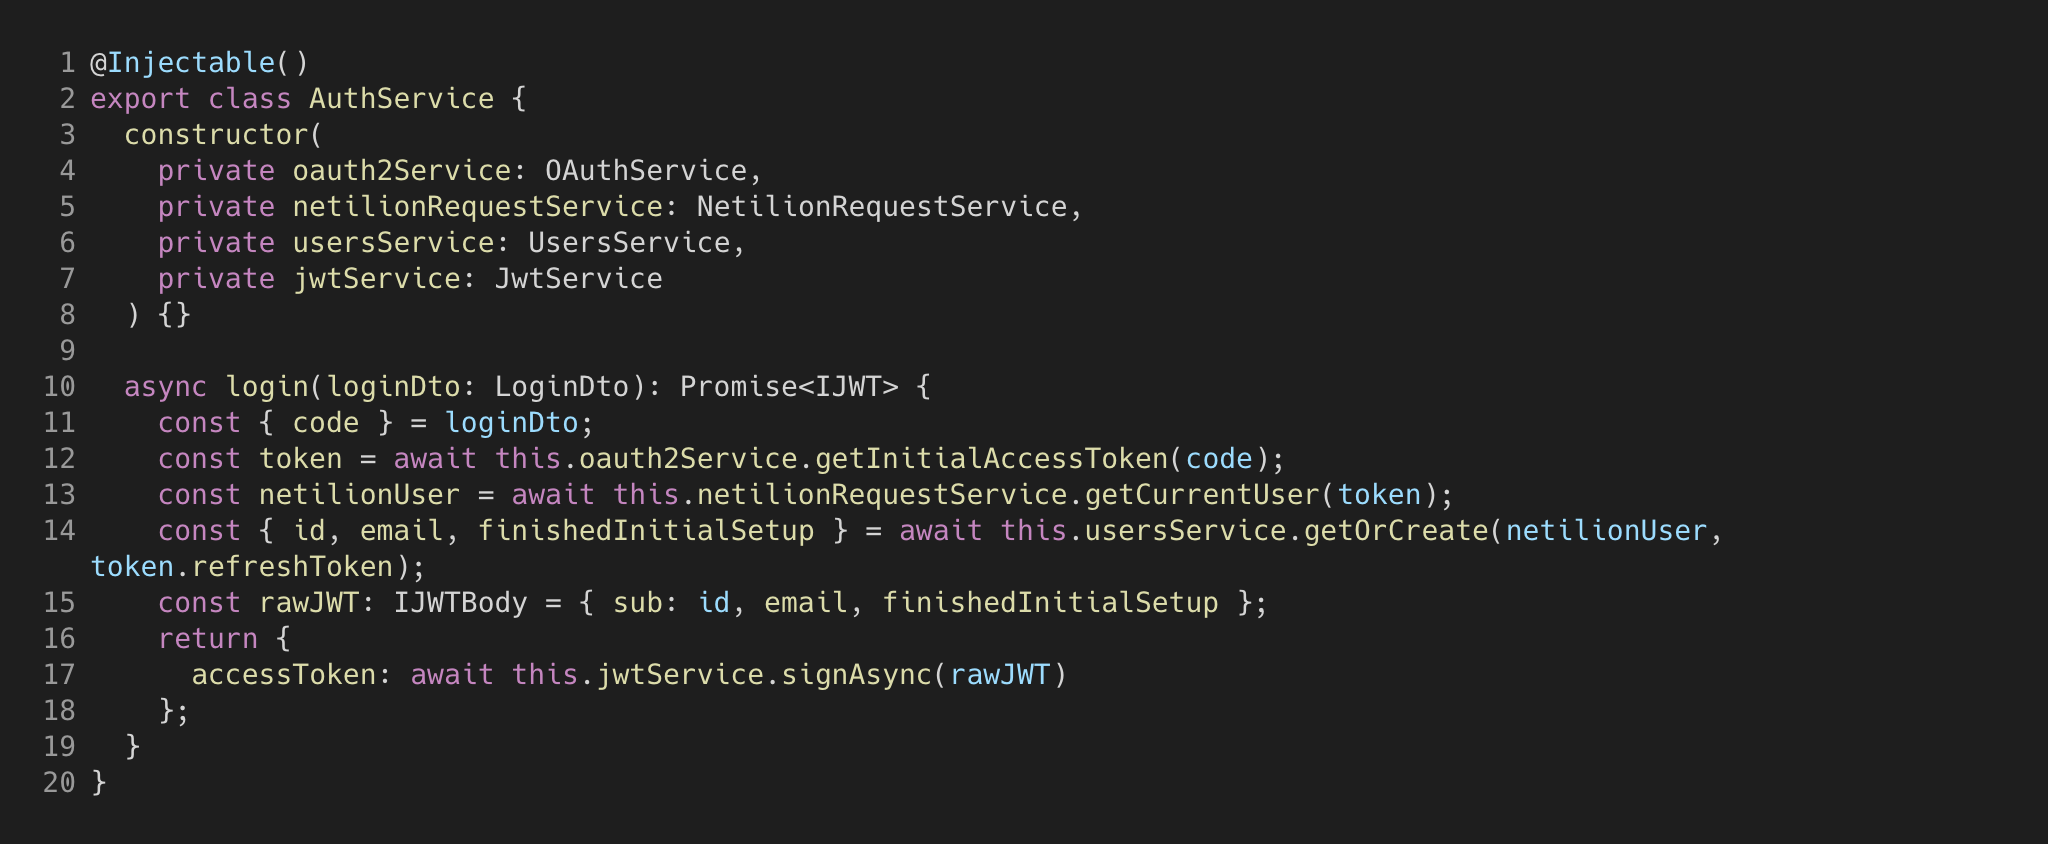
\includegraphics[width=.95\linewidth]{./images/auth.service.ts.png}
  \caption[{auth.service.ts von \code{ose-dashboard-bcknd}}]{auth.service.ts von \code{ose-dashboard-bcknd}}
  \label{fig:auth-service}
\end{figure}
Das Frontend erhält bei einer erfolgreichen Anmeldung einen Code. Dieser Code sendet es weiter an das Backend. Als erstes wird der Code in einen Token umgewandelt. Mit diesem Token ist es nun möglich die Nutzerinformationen von Netilion abzufragen. Anschliessend wird die Function \code{getOrCreate} vom \code{usersService} mit den Nutzerinformationen und dem Token aufgerufen. Diese Funktion fragt zuerst bei der Datenbank nach, ob der Nutzer bereits existiert. Existiert er, wird er direkt zurückgeben. Existiert er nicht, wird ein neuer erstellt.
Danach werden die für den JWT-Payload nötigen Daten in einem Objekt gebündelt und vom \code{jwtService} in einen signed JWT formattiert.
\newline
Der JWT wird als Antwort auf die Anfrage zurück ans Frontend gesendet, wo er fortlaufend, wie in Kapitel \ref{andwendung-jwt} beschrieben, als Authentifizierungsmethode zwischen Front- und Backend verwendet wird.
\subsubsection{Assets}
\begin{figure}[H]
  \centering
  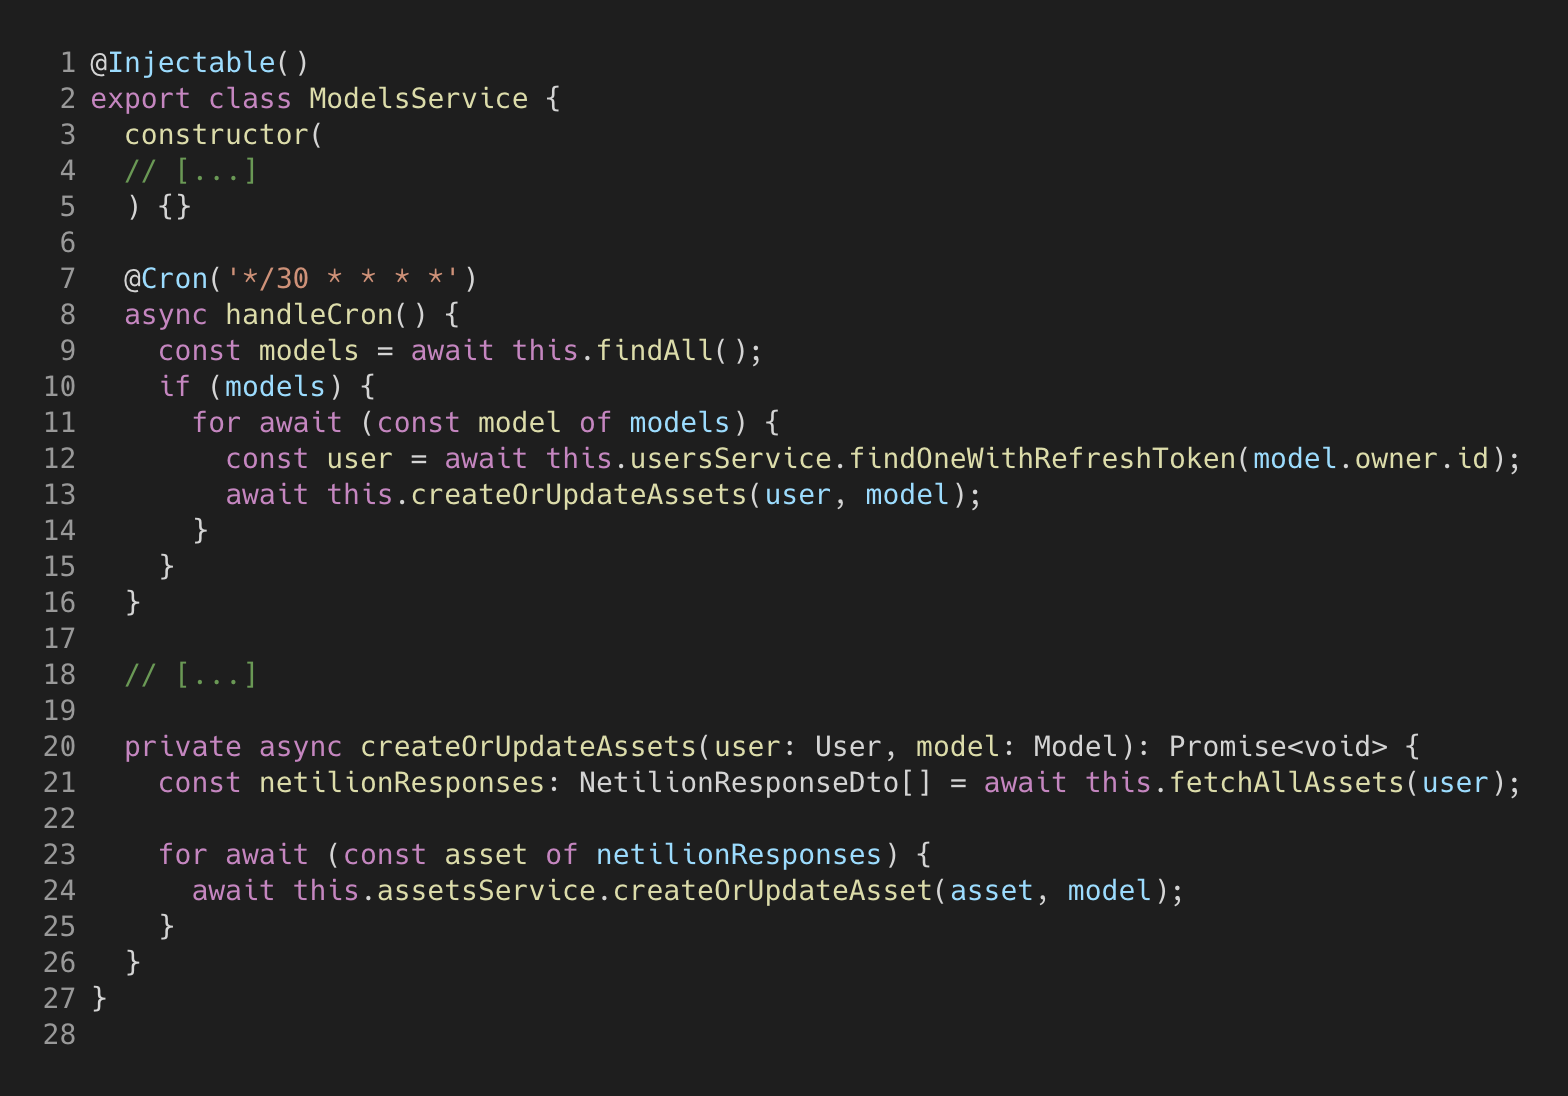
\includegraphics[width=.95\linewidth]{./images/models.service.ts.png}
  \caption[{models.service.ts von \code{ose-dashboard-bcknd}}]{models.service.ts von \code{ose-dashboard-bcknd}}
  \label{fig:models-service}
\end{figure}
Im \code{ModelsService} ist von Zeile sieben bis 16 ein Cron-Job deklariert. Dieser ist so konfiguriert, dass die \code{handleCron} Funktion auf Zeile acht alle 30 Minuten aufgerufen wird. Diese Funktion fragt zuerst beim Repository alle Modelle nach. Anschliessend wir in einer Schleife von jedem Modell der dazugehörige Nutzer abgefragt, womit danach die Funktion \code{createOrUpdateAssets} aufgerufen wird.
\newline
Diese Funktion fragt zuerst bei Netilion nach allen Assets des Users nach. Nachdem die Antwort erhalten wurde, schleift sie über alle Assets und ob diese erstellt werden müssen oder einfach aktualisiert werden können.
\section{Account löschen}
Normalerweise kann man sich bei einem Dienst wieder abmelden und dank GDDPR auch alle seine Daten löschen lassen. In unserem Fall sollte der \code{refresh\_token} des OSE-Verantwortlichen revoked werden, woraufhin die Entität gelöscht wird. Im optimalen Falle sollte das ORM so konfiguriert sein, dass danach alle Daten kaskadierend gelöscht werden. Das bedeutet, dass alle Einträge in der Datenbank, welche mit dem User in Verbindung gebracht werden können, nacheinander gelöscht werden.
\newline
Da dies ein bedeutender Auwand ist, welcher nicht von dieser IPA verlangt wird, werde ich dies nach der Abschlusspräsentation implementieren.
\section{Modellauswahl}
Es wurde schon bei Kapitel \ref{mck:index} auf die Abbildung \ref{fig:mck-index} eingegangen, dabei wurde jedoch ein Punkt bewusst weggelassen. Die Fläche, welche mit \amk{Model selection} markiert ist, soll nicht einfach leer sein, sondern dem Nutzer das Navigieren der Modelle einfach zu machen.
\newline
Bei den Mockups wurde allerdings das ganze noch nicht verfeinert, da mögliche Lösungen zuerst evaluiert werden sollen. Momentan stehen zwei Möglichkeiten zur Auswahl bereit. Diese werden in den Kapiteln \ref{mdlauswl-a} und \ref{mdlauswl-b} beschrieben.
\subsection{Auflistung mit Landesflaggen} \label{mdlauswl-a}
Die initiale Idee der Modellauswahl war eine Auflistung der Modelle nach den Ländern. Damit ich dies im Frontend machen kann, muss ich zuerst im Controller der Modelle eine neue Route implementrieren, welche sie nach den Ländern geordnet zurücksendet.
\newline
Meiner Meinung nach ist diese Möglichkeit sehr simpel, was nicht negativ gemeint ist. Sollte ich merken, dass die andere Möglichkeit Probleme macht oder machen könnte, werde ich diese implementieren.
\subsubsection{Pro}
\begin{itemize}
  \item Einfach zu implementieren
  \item Erfüllt den Zweck
  \item Lauft etwas schief, kann ich mir selbst weiterhelfen
\end{itemize}
\subsubsection{Kontra}
\begin{itemize}
  \item Eine dynamische Darstellung von Flaggen, in der Form von Bildern oder Emojis, könnte sich als schwieriger als Gedacht herausstellen
  \item Schwierig schön darzustellen
  \item Mehr Fleissarbeit um dies zu implementieren
\end{itemize}
\subsection{Interaktive Weltkarte} \label{mdlauswl-b}
Eine Idee die von mir kommt, ist die Darstellung mit einer Weltkarte. Ich hatte diese Idee bevor die IPA begann und habe mich in der Freizeit weiter informiert. Zuerst dachte ich, ich könne eine Karte im SVG-Format nehmen und selbst eine solche React-Komponente erstellen. Schnell wurde klar, dass sich dies als sehr grosser Aufwand herausstellen würde. Dadurch begann ich mit der recherche nach Libraries von Dritten, welche sich diese mühe bereits gemacht haben. Somit stiess ich auf \href{https://www.react-simple-maps.io/}{\code{react-simple-maps}}.
\newline
Mit dieser Komponente ist es mir möglich, eine Weltkarte mit Markern darzustellen. Die Marker werden dabei mit Koordinaten gesetzt. Da ich bei der Registration die Koordinaten des Modells erhalte, sollte dies kein Problem sein.
\subsubsection{Pro}
\begin{itemize}
  \item Ohne Konfigurationen sieht diese Komponente schön aus
  \item Weniger Fleissarbeit um dies zu implementieren
\end{itemize}
\subsubsection{Kontra}
\begin{itemize}
  \item Ich muss mich etwas in die Dokumentation einlesen
  \item Lauft etwas schief, kann mir nur Google oder die Dokumentation weiterhelfen
\end{itemize}
\subsection{Tatsächliche Auswahl}
Bei der Implementierung wird nun zweitere Möglichkeit, welche in Kapitel \ref{mdlauswl-b} beschrieben wurde, implementiert. Grund dafür ist, dass genügen Zeit zur verfügung ist und nicht eine overengineerte Lösung gebastelt werden muss, welche kurz nach der IPA ersetzt wird. Begründet wird dieser Entscheid damit, dass die Dokumentation im Aspekt der Verwendung in diesem Projekt gründlich durchgelesen wurde. 
\section{Automatische Verlinkung von Assets und Meshes}
Eine Anforderung dieser IPA ist, dass die Verlinkun von Assets und Meshes automatisch gemacht werden kann. Dies ist möglich, da sich bereits alle benötigten Informationen in der Datenbank des Backends befinden. Dies soll so die Erfahrung des Benutzer fördern und den Registrationsprozess vereinfachen.
\begin{figure}[H]
  \centering
  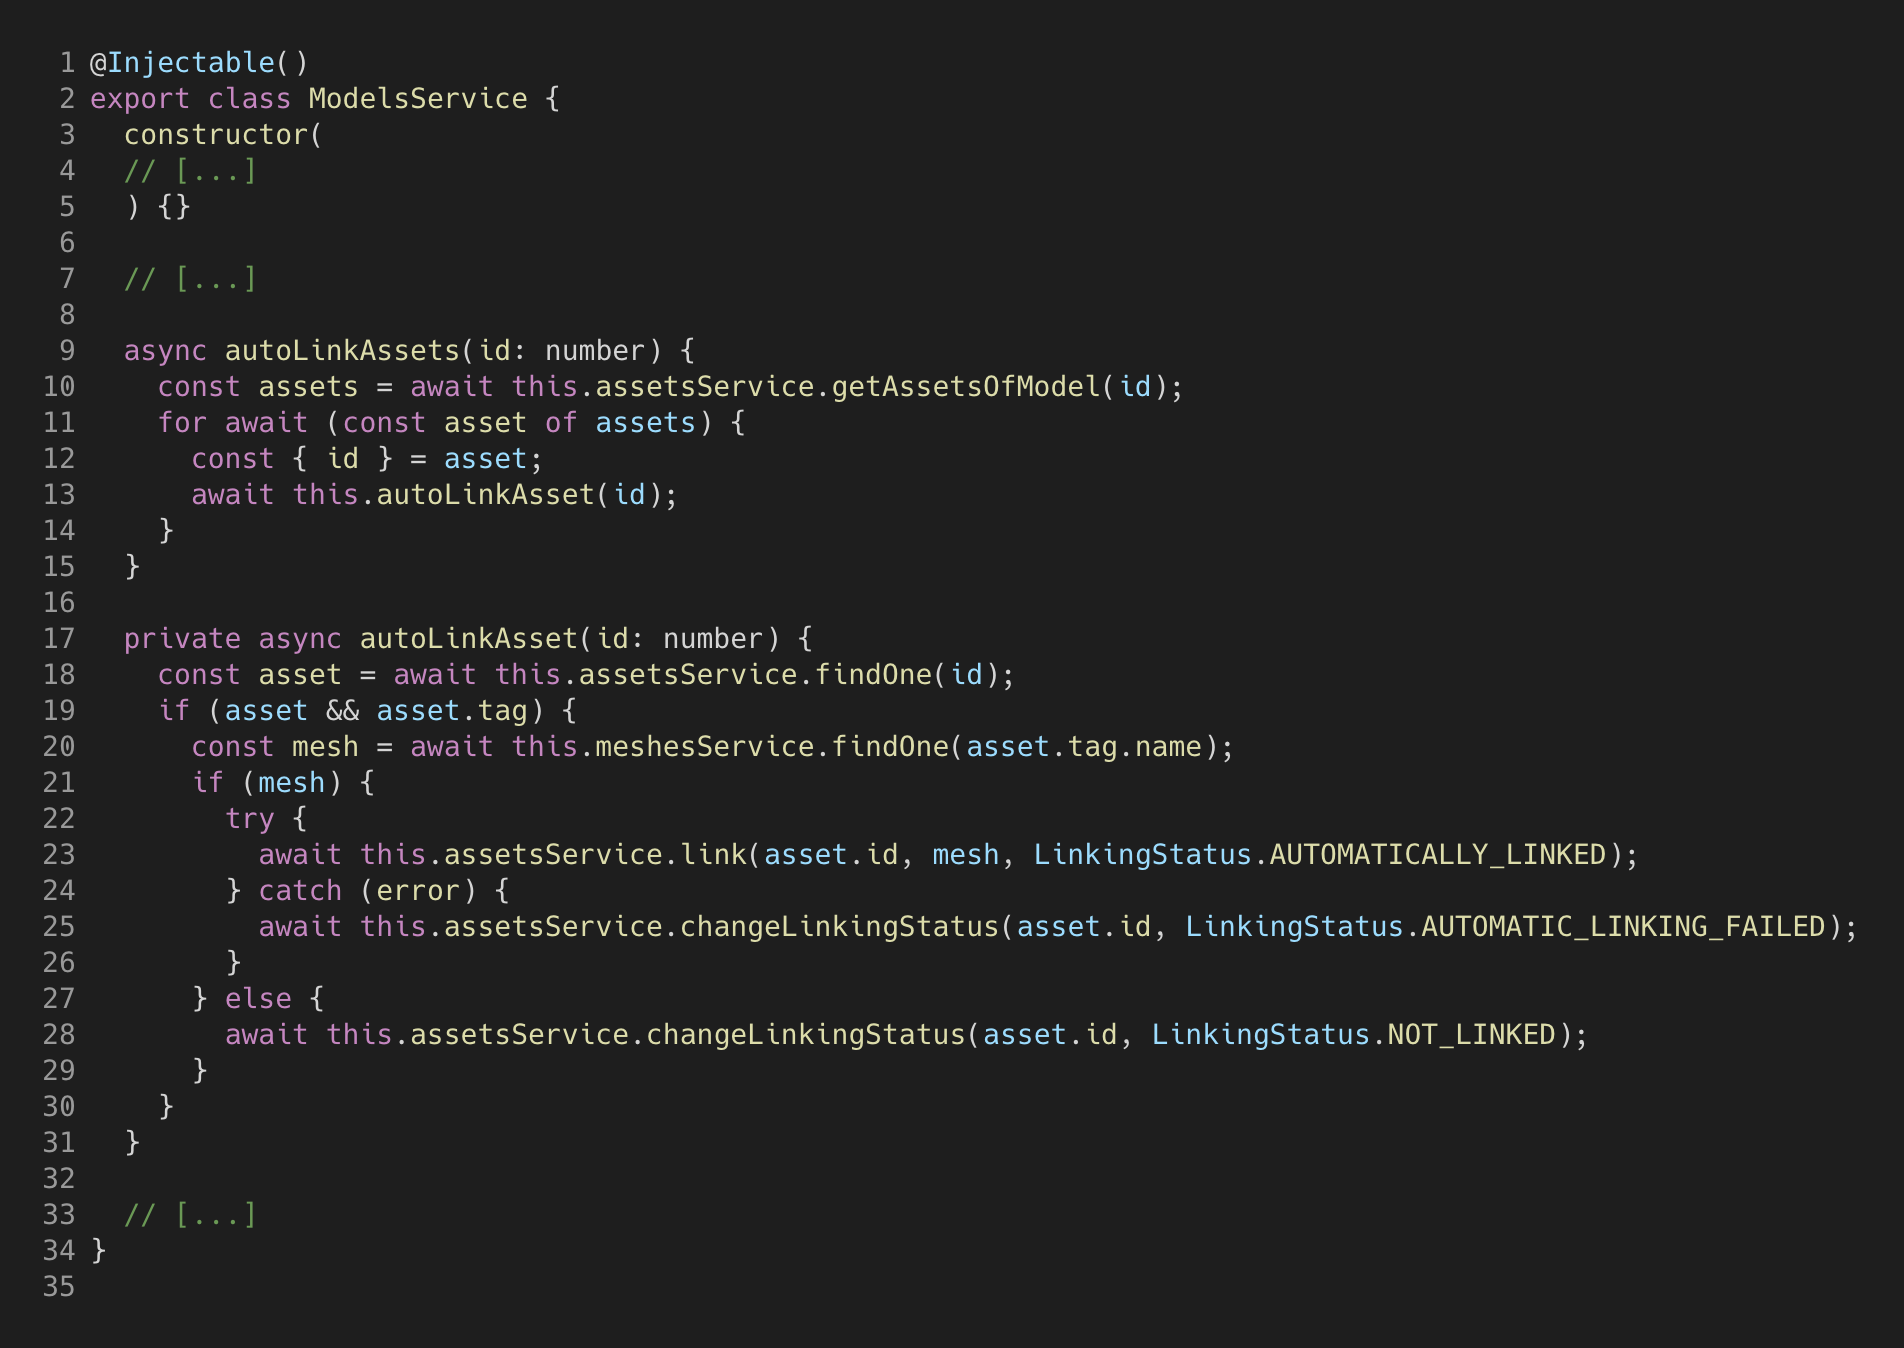
\includegraphics[width=.95\linewidth]{./images/models.service.ts.2.png}
  \caption[{models.service.ts von \code{ose-dashboard-bcknd}}]{models.service.ts von \code{ose-dashboard-bcknd}}
  \label{fig:settingsLayout}
\end{figure}
Die Funktion \code{autoLinkAssets} schleift über alle Assets eines Modells und ruft dabei für jedes einzelne \code{autoLinkAsset} auf. Diese erstellt die wirkliche Verlinkung. Dafür fragt es das Asset zuerst einzeln beim \code{assetsService} nach, da auf diesem Weg die Relation zu \code{Tag} left joined und selektiert wird. Wurde ein Asset mit einem Tag gefunden, wird beim \code{meshesService} nachgefragt, ob ein Mesh mit dem Namen des Tags existiert. Ist dies der Fall, werden die beiden miteinander verlinkt.
\section{Einhaltung der Coding Guidelines}
Die Coding Guidelines wurden eingehalten. Der Linter zeigt auf dem Front- und Backend weder Errors noch Warnings an. Es ist wichtig zu erwähnen, dass die Regeln nicht angepasst wurden und es keine Instanz gibt, an der eine Regel ignoriert wurde.
\newline
Dies kann bei beiden Repositories mit dem Kommand \code{yarn lint} überprüft werden.
\begin{figure}[H]
  \centering
  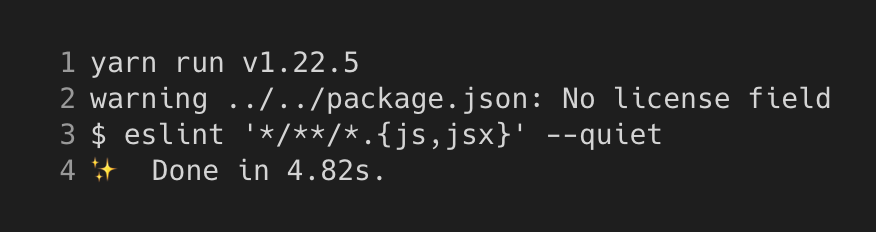
\includegraphics[width=.7\linewidth]{./images/linting-frontend.png}
  \caption[{Output von \code{yarn lint} im Frontend}]{Output von \code{yarn lint} im Frontend}
  \label{fig:lint-frnt}
\end{figure}
\begin{figure}[H]
  \centering
  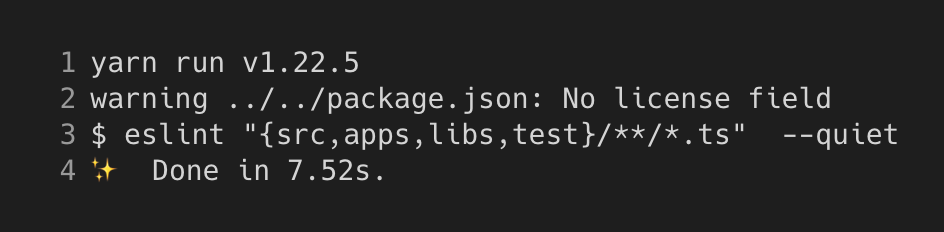
\includegraphics[width=.7\linewidth]{./images/linting-backend.png}
  \caption[{Output von \code{yarn lint} im Backend}]{Output von \code{yarn lint} im Backend}
  \label{fig:lint-bck}
\end{figure}
Eine Anmerkung muss hierbei gemacht werden. Die \amk{Warning} die in den Abbildungen \ref{fig:lint-frnt} und \ref{fig:lint-bck} bezieht sich nicht auf das Linting. Es handelt sich dabei um eine Warnung des Packetmanagers \amk{NPM}. Dieser wirft die Warnung, da ihm die Lizens in der Datei \code{package.json} unbekannt ist. Da es sich bei dieser Arbeit um kein öffentliches Projekt handelt, habe ich \code{\amk{license}: \amk{UNLICENSED}} angegeben.
\section{Umgebungsvariablen}
Umgebungsvariablen sind für fast alle Webanwendung nötig. Sie machen es möglich geheime oder heikle Daten der Anwendung erst zur Laufzeit zur Verfügung zu stellen. Auf diese Weise müssen die Daten nicht im Code fest angegeben werden. So kann ein Versionskontrollsystem eingesetzt werden, ohne das Dritte an heikle Daten kommen. Folgend sind die verwendeten Umgebungsvariablen beschrieben.
\subsection{Umgebungsvariablen - Frontend}
\begin{table}[H]
  \begin{tabularx}{\textwidth}{X X}
  \textbf{Variable} & \textbf{Beschreibung} \\ \\\hline \\
  NEXT\_PUBLIC\_AUTH\_URL & Die URL, auf die der Benutzer während dem Anmeldeprozess weitergeleited wird \\
  NEXT\_PUBLIC\_API\_BASE\_URL & URL, welche auf eine Instanz des Backends zeigt. \\
  \\\hline
  \end{tabularx}
\end{table}
\subsection{Umgebungsvariablen - Backend}
\begin{table}[H]
  \begin{tabularx}{\textwidth}{X X}
  \textbf{Variable} & \textbf{Beschreibung} \\ \\\hline \\
  PORT & Der Port unter dem das Backend erreichbar ist \\
  DATABASE\_URL & Datenbankverbindungsadresse \\
  NETILION\_AUTHURL & Basis URL für Anfragen an den OAuth2 Endpoint \\
  NETILION\_AUTHURL & Basis URL für Anfragen an den OAuth2 Endpoint \\
  NETILION\_URL & Basis URL für Anfragen an die Resourcen Endpoints \\
  NETILION\_REDIRECT\_URI & URI, auf die der User nach dem Anmeldeprozess weitergeleited wird \\
  NETILION\_CLIENT\_ID & Id der erstellten OAuth2 Applikation in Netilion \\
  NETILION\_CLIENT\_SECRET & Secret der erstellten OAuth2 Applikation in Netilion \\
  REDIS\_URL & Redis Verbindungsadresse \\
  REDIS\_TTL & Gibt an, wie lange Einträge in Redis gespeichert bleiben \\
  SECURITY\_JWT\_SECRET & String, mit welchem die JWTs signiert werden \\
  SECURITY\_JWT\_EXPIRES\_IN & Gibt an, wie lange JWTs gültig sind \\
  SECURITY\_JWT\_EXPIRES\_IN & String, mit welchem die \code{refresh\_token} verschlüsselt werden \\
  GEOLOCATION\_API\_KEY & Zugriffsschlüssel, um auf die \amk{HERE Developer API} zugreifen zu können \\
  PERMITTED\_USERGROUP\_ID & Id der Netilion UserGroup. Nur die darin enthaltenen Nutzer können sich anmelden \\
  PERMITTED\_USERGROUP\_NAME & Name der Netilion UserGroup. Nur die darin enthaltenen Nutzer können sich anmelden \\
  \\\hline
  \end{tabularx}
\end{table}
\section{3D Modell auswechseln}
In der ersten Version des OSE-Dashboards stellte sich die korrekte Einbindung des Modells als schwierig heraus. Grund dafür ist, dass die Datei mehrmals mit speziellen konfigurationen umgewandelt werden muss. Diese Schritte sind in diesem Kapitel beschrieben, damit nachfolgende Entwickler/-innen sich die Mühe und Zweit ersparren können.
\begin{enumerate}
  \item Das Model wird von einem Konstrukteur von Endress+Hauser erstellt. Da Konstrukteure CAD-Modelle modellieren, wird die Datei mit hoher wahrscheinlichkeit vom Typ .stp sein.
  \item Wird ein Auftrag beim Konstrukteur erstellt, muss dieser darauf hingewiesen werden, dass die einzelnen Bestandteile des Modells für uns korrekt benannt werden müssen. Im Schritt 10 ist es sehr wichtig, dass die Benennung keine Umlaute (öäü) und Leerzeichen enthält.
  \item Für die erste Umwandung wird das Program \amk{FreeCAD} verwendet. Dieses muss auf einem Windows Computer installiert werden.
  \item Die .stp Datei importieren und als .dae exportieren
  \item Für die nächste Umwandung brauchen wir eine 3D Modellierungssoftware. Bisher wurde Blender verwendet, da dies keine Kosten verursacht.
  \item In Blender kann das Modell nun nach belieben angepasst werden. Zum Beispiel können Farben verändert werden.
  \item Anschliessend soll das Modell als .gltf exportiert werden. In diesem Schritt kann der Detailgrad bestimmt werden. Je höher der Detailgrad desto grösser ist die Datei. Eine grosse Datei verlangsamt die Ladezeit erheblich und erfordert moderne Hardware um flüssig angezeigt werden zu können.
  \item Nun kann die .gltf Datei in den \amk{public} Ordern von React/Nextjs gelegt werden. Dies ist notwendig, da der Client des Benutzers diese Datei herunterladen können muss.
  \item Für den nächsten Schritt brauchen wir ein Script. Das Repository dafür ist \href{https://github.com/pmndrs/gltfjsx}{\code{pmndrs/gltfjsx}}. Dieses muss nicht installiert werden, sondern kann als Remote Script mit NPM ausgeführt werden. In der Dokumentation des Scriptes ist die korrekte Anwendung beschrieben.
  \item Nun sollte mit gltfjsx aus der .gltf Datei eine React Komponente generiert werden. Diese sollte in den \amk{components} Ordner verschoben werden.
  \item Um das Modell darzustellen, muss das Modell in der Scene Komponente eingebunden werden.
  \item Damit das Modell interaktiv wird, müssen noch einige kleine konfigurationen gemacht werden. Die Szene enthält eine Variable \amk{assetSelected}. Diese muss der Modell Komponente als property weitergegeben werden.
  \item Anschliessend müssen die Meshes im Modell, welche ein Asset darstellen, durch die Komponente \amk{Asset} ersetzt werden und mit zusätzlichen Informationen ausgestattet werden. Dies wird in der Abbildung \ref{fig:mdl-cmpnt} dargestellt.
\end{enumerate}
\begin{figure}[H]
  \centering
  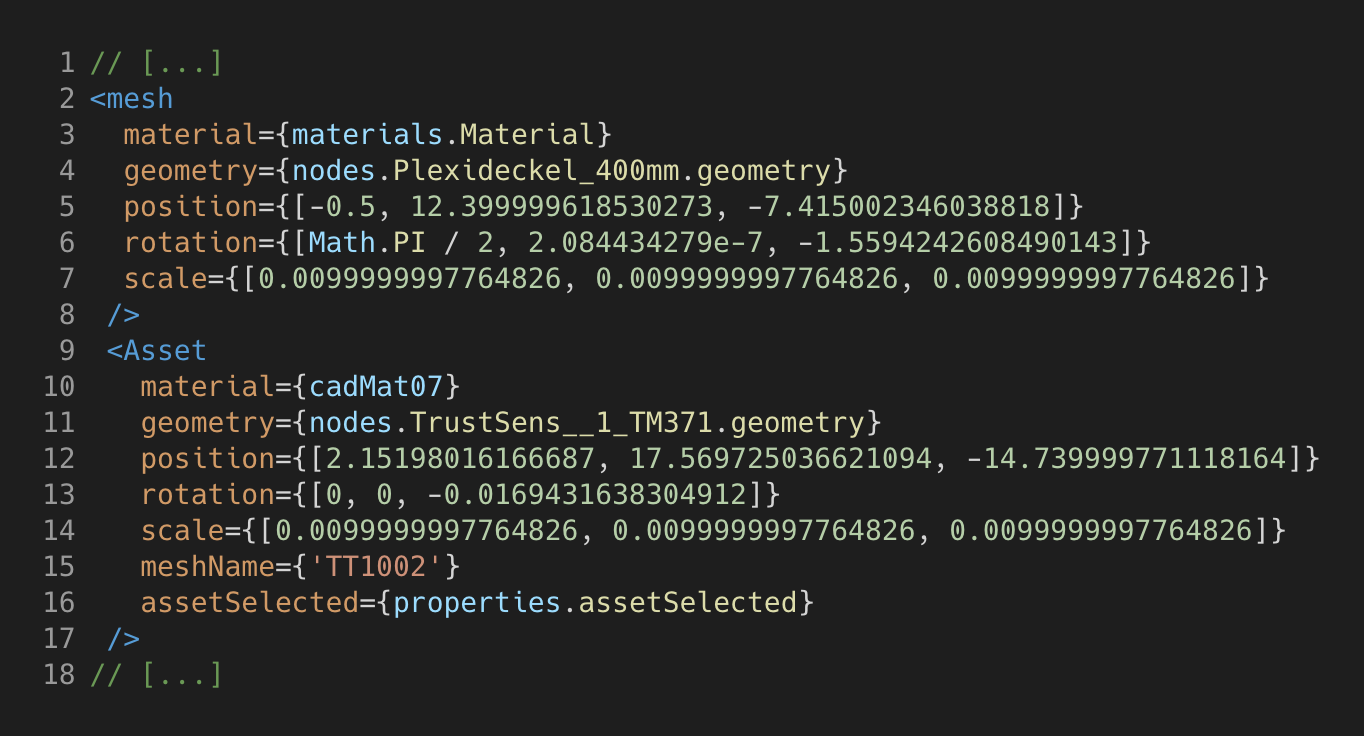
\includegraphics[width=.7\linewidth]{./images/model.js.png}
  \caption[{Ausschnitt aus der momentanen \amk{Model.js} Komponente}]{Ausschnitt aus der momentanen \amk{Model.js} Komponente}
  \label{fig:mdl-cmpnt}
\end{figure}
Die \amk{Asset} Komponente besteht aus einem Mesh. Daher werden auch alle Properties des Meshes verlangt. Zusätzlich muss der Mesh mit einem Tag benannt werden. Damit die hierarchisch höher liegende Komponente erkennen kann, wann welches Asset angeklickt wurde, muss noch die Funktion \amk{assetSelected} mitgegeben werden.

Mit diesem Schritt ist die einbundung eines neuen Modelles abgeschlossen.

\chapter{Testen}
Das Testen der fertigen Applikation wurde am 13.04.2021, wie im Kapitel \ref{testkonzept} geplannt, durchgeführt. Die Ergebnisse sind im folgendem Kapitel \ref{test-ergebnisse} dokumentiert.
\section{Testergebnisse} \label{test-ergebnisse}
\begin{table}[H]
  \begin{tabularx}{\textwidth}{l X l}\hline \\
  \textbf{Kapitel} & \textbf{Test-Case} & \textbf{Fehlerklasse} \\ \\\hline \\
    \ref{tc-01} & TC-01: Login & 0 \\
    \ref{tc-02} & TC-02: Login falsche Logindaten & 0 \\
    \ref{tc-03} & TC-03: Login mit unberechtigtem Account & 0 \\
    \ref{tc-04} & TC-04: Automatische Verlinkung der Assets & 1 \\
    \ref{tc-05} & TC-05: Konfigurationsmenü aufrufbar & 0 \\
    \ref{tc-06} & TC-06: Verlinkung manuell änderbar & 0 \\
    \ref{tc-07} & TC-07: Übersicht aller Standorte & 0 \\
    \ref{tc-08} & TC-08: Standort änderbar & 0 \\
  \\\hline
  \end{tabularx}
\end{table}
\chapter{Abschluss} \label{abschluss}
\section{Bekannte Fehler}
\subsection{Konfigurationsmenü}
Durch das Konfigurationsmenü kann die Applikation momentan vom einem Benutzer zum abstürzen gebracht werden. Grund dafür ist das komplexere State Management, welches noch nicht 100\% durchgedacht wurde. Mit bestimmten Interaktionen kann ein Fehler auftreten, welcher im momentanen Stand nicht behandelt wird. Dies sorgt so für einen Absturz.
Allerdings wird die Funktionalität der Applikation dadurch nicht beeinträchtigt, da durch das \amk{normale} interagieren der Fehler nicht auftritt.
\subsection{Verlinkung von Assets zu Meshes}
Die automatische und manuelle Verlinkung funktioniert und die Applikation ist nutzbar. Jedoch gibt es einige Edge Cases durch welche auffält, dass die Implementation noch nicht ganz perfekt ist. Grund hierfür ist die darunterliegende Datenstrucktur.

Die Abbildung \ref{fig:db-erweiterung} stellt dar, dass ich in der Vorarbeit die Tabellen \amk{asset}, \amk{product}, \amk{tag} und \amk{status} bereits erstellt habe. Die Priorität war damals, dass alle Daten in die Datenbank übernommen werden und dadurch so wenig Anfragen wie möglich an Netilion gesendet werden. Dazu kommt noch, dass die Schnittstelle für die Assets gleich noch die Informationen der restlichen drei Tabellen mitsenden kann, ohne das man mehrere Requests machen muss. Umgekehrt, also vom Tag zum Asset geht dies nicht.

Durch diese Vorbedingungen/Erfahrungen spielte die Asset Tabelle eine zentrale Rolle im Datenbankschema. Dies stellte sich später allerdings als negativ heraus. Die vorgeschlagene Lösung enthielt eine Hilfstabelle namens \amk{mesh}, womit ein Asset verlinkt werden sollte. Durch diese Implementation ist es nun möglich, dass mehrere Assets des gleichen Modelles mit demselben Mesh verlinkt sind.

Eine bessere Lösung wäre es, wenn der Tag die zentrale Rolle übernehmen würde. Dadurch würde die Hilfstabelle \amk{mesh} nicht mehr verwendet werden müssen. Ausserdem könnte so ein Asset nur mit einem Mesh verlinkt werden, was die Fehleranfälligkeit vermindert.

Dies zu Ändern hätte allerdings den Rahmen einer IPA deutlich gesprengt. Gerne werde ich nach der IPA das ganze genauer analysieren und implementieren.
\section{Verbesserungsmöglichkeiten}
\subsection{Layout verschiebungen}
Es kommt im Frontend momentan sehr oft zu Layout verschiebungen. Damit gemeint ist, dass Elemente, mit dennen der User interagieren möchte, durch State Changes die Position verändern. Aus User Experience Sicht ist dies schlecht gelöst. Beispiel hierfür ist das Vorschlagen von Adressen. Sobald der User einen Teil einer Adresse eingibt, erscheinen drei bis fünf Vorschläge. Diese Vorschläge schieben andere Elemente wie Eingabefelder weiter nach unten.

Dieses Problem kann in React sehr schön und einfach mit dem Drittanbieterpacket \href{https://www.framer.com/motion/}{\code{framer-motion}} gelöst werden. Ich habe bereits Erfahrungen damit gesammelt und würde gerne nach der IPA dies Implementieren.
\subsection{Refresh Token verschlüsseln}
Im Dokument ist erwähnt, dass der \code{refresh\_token} des Benutzers verschlüsselt in der Datenbank gesichert wird. Dies hatte während der Implementierungsphase eine niedrige Priorität, da es nicht direkt zur Funktionalität beitrug. Nun bleibt keine Zeit mehr für die Implementation. Ich werde dies baldmöglichst nach der IPA implementieren, da mir die Sicherheit der Applikation sehr wichtig ist.
\subsection{Unit test/-s}
In der Aufgabenstellung stand, dass die Methode, welche die Assets mit Meshes verlinkt, mit automatischen Tests abgedeckt werden soll. Mit Tests habe ich in Nestjs sehr wenig Erfahung, wodurch mich eine Implementation des Testes einiges an Zeit gekostet hätte. Ich habe dies nun bewusst weggelassen, damit ich mich auf andere Aufgaben fokussieren kann.
\section{Verstösse gegen die Coding Guidelines}
\subsection{Frontend}
\subsubsection{/pages/settings/location.js:19}
\begin{figure}[H]
  \centering
  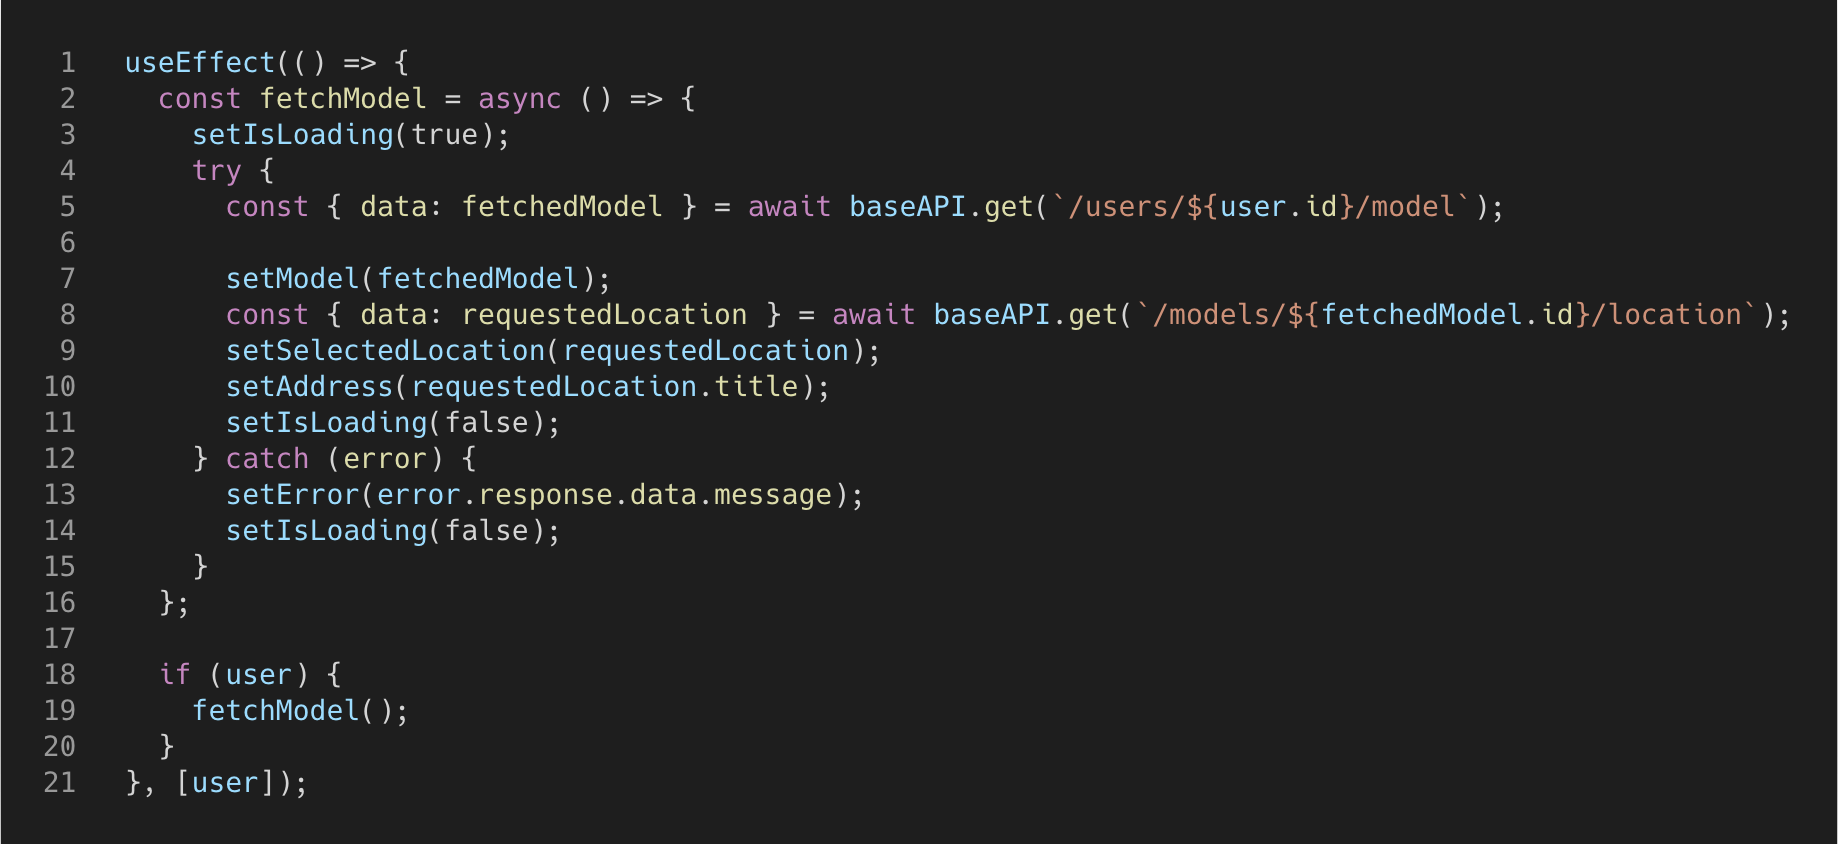
\includegraphics[width=.95\linewidth]{./images/verstoss-1.png}
  \caption[{Abbildung der useEffect Hook in location.js}]{Abbildung der useEffect Hook in location.js}
\end{figure}
Dieser Verstoss ist zu Begründen auf die vielen State updates die innerhalb der useEffect Hook geschehen. Dies ist nicht wirklich sinnvoll auslagbar.
\subsubsection{/pages/settings/model.js:16}
\begin{figure}[H]
  \centering
  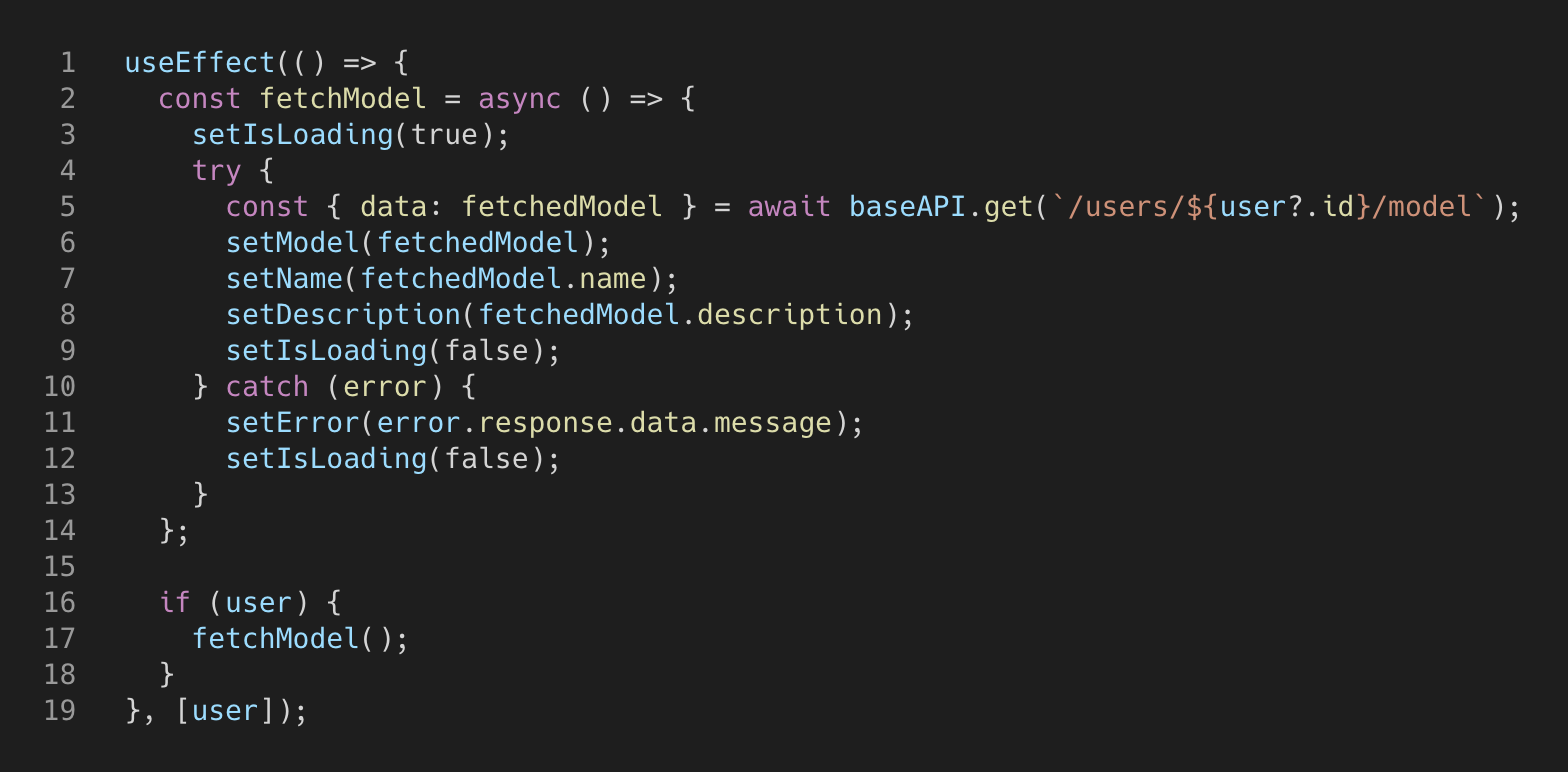
\includegraphics[width=.95\linewidth]{./images/verstoss-2.png}
  \caption[{Abbildung der useEffect Hook in model.js}]{Abbildung der useEffect Hook in model.js}
\end{figure}
Dieser Verstoss folgt der gleich gleichen Begründung wie der erste.
\subsection{Backend}
\subsubsection{/src/netilion-request/netilion-request.service.ts:43}
\begin{figure}[H]
  \centering
  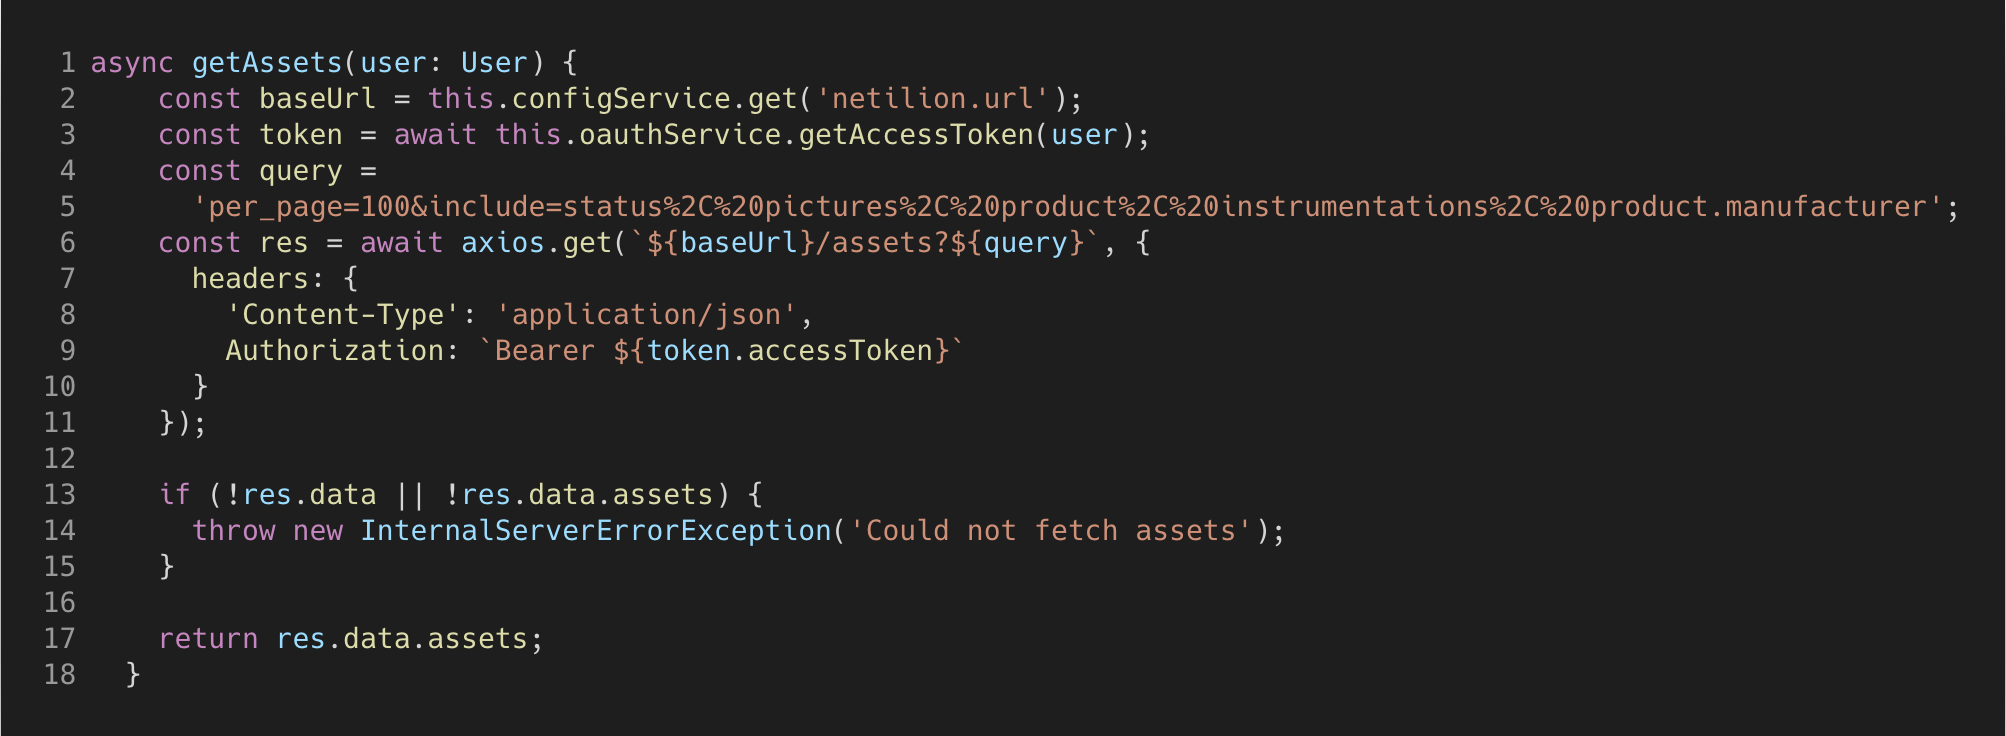
\includegraphics[width=.95\linewidth]{./images/verstoss-3.png}
  \caption[{Abbildung der getAssets Funktion}]{Abbildung der getAssets Funktion}
\end{figure}
Bei dieser Funktion handelt es sich bereits um eine Auslagerung. Jede Zeile muss in dieser Funktion sein und ist sinnlos auszulagern.
\subsubsection{/src/netilion-request/oauth.service.ts:18\&43}
Auch bei diesen Funktionen handelt es sich um ausgelagerte Rest Abfragen. Jegliche Teile auszulagern würde nur den Code schwerer zum Verstehen machen.
\section{Schlussbetrachtung}
\subsection{Reflexion}
Wie man vielleicht den Arbeitsjournalen ablesen konnte, war ich in den vergangen zehn Tagen durchgehend in Stresssituationen. Rückblickend gesehen, hätten wir den Auftrag etwas kürzen können. Ich hatte auch am Anfang der Implementierungsphase extremen Respekt davor, dass ich den Anmeldeprozess mit OAuth2 nicht schaffen werde. Beziehungsweise das es mir viel zu viel Zeit wegnehmen könnte, sodass ich folglich zu wenig Zeit für andere Aufgaben hätte. Dies ist zum Glück nicht aufgetreten und es verlief alles recht positiv.
\subsection{Schlusswort}
Ich konnte mit dieser Arbeit eine grosse Erweiterung des OSE-Dashboards erstellen. Diese kann nun von verschiedenen Endress+Hauser Standorten eingesetzt werden, um den Kunden die Möglichkeiten von Netilion Connect näher zu bringen.
\subsection{Persönliche Bilanz}
Ich bin mir sicher, dass ich einige Erfahrungen dieser Arbeit in mein weiteres Berufsleben mitnehmen kann. Ich konnte unter Druck arbeiten, wobei meine Leistung in den ganzen zehn Tagen nicht abgenommen hat. Ich hatte viele Momente in diesen Tagen, an dennen ich am liebsten einfach nichts gemacht hätte für ein bis zwei Stunden, da ich so unter Druck stand. Jedoch habe ich es durchgezogen und merkte dadurch, dass dies nur eine kleine gedankliche Barrier war, die ich überweltigen konnte.
Abgesehen davon investierte ich sehr viel Zeit in diese Technische Dokumentation. Ich denke auch hier, dass mir gewisse Erfahrungen und Eindrücke bleiben werden.
Ausserdem habe ich mit dieser Arbeit eine nahezu perfekte Implementation von OAuth2 im Bezug auf den Anmeldeprozess erstellt.

Ich bin mehr als nur zufrieden mit meinen erreichten Ergebnissen.

  \part{Anhang}
  \begin{appendix}  
  % \chapter{Abkürzungsverzeichnis}

\begin{acronym}[OSE]
  \acro{ose}[OSE]{One Story Exhibit}
  \acro{sc}[SC]{Sales Center}
  \acro{spa}[SPA]{Single Page Application}
\end{acronym}

  \chapter{Glossar}
\begin{table}[H]
  \begin{tabularx}{\textwidth}{l X}\hline \\
  \textbf{Ausdruck} & \textbf{Erklärung}  \\ \\\hline \\
  Angular & TypeScript Frontend Framework \\
  API & Applikation Programming Interface - Eine Softwareschnittstelle zwischen getrennten Schichten \\
  Asset & Endress+Hauser interne Bezeichnung für ein Messgerät \\
  Backend & Softareschicht, welche sich um die Bussiness Logik und serialisierung der Daten kümmert \\
  Branches & Entwicklungslinien \\
  Build-Pipelines & Coninous Delivery Anwendung \\
  CI/CD & Continous Integration/Coninous Delivery \\
  Edge Device & Gerät, welches Daten von den Messgeräten abliest und in Netilion schreibt \\
  Express.js & JavaScript Backend Bibliothek \\
  Frontend & Softwareschicht, welche sich um die Darstellung von Daten und Prozessen kümmert \\
  GDDPR & Datenschutzgesetz der EU \\
  Git & Versionskontrollsoftware \\
  HERE Developer API & Drittanbieter Schnittstelle \\
  Heroku & Hostinganbieter des Backends \\
  IIoT & Industrial Internet of Things \\
  IIoT-Ökosystem & Ganzes IIoT angebot von Netilion \\

  \\\hline
  \end{tabularx}
\end{table}
\pagebreak
\begin{table}[H]
  \begin{tabularx}{\textwidth}{l X}\hline \\
  \textbf{Ausdruck} & \textbf{Erklärung}  \\ \\\hline \\
  IPA & Individuelle Praktische Arbeit \\
  JSX & React Syntax - Vermischung von HTML und JavaScript wird ermöglicht \\
  Kanban & Projektmanagementmethode \\
  Lucidchart.com & Website mit der Diagramme erstellt werden können \\
  Mesh & Ein Teil eines 3D Modells \\
  Microsoft Projekt & Tool, welches für die Erstellung des Projektplanes eingesetzt wurde \\
  Mockups & Designentwurf einer Website \\
  MVT & Auftraggeber dieses Projektes \\
  NE107 Status & Standartisierter Status, welcher den Zustand eines Messgerätes beschreibt \\
  Netilion & IIoT PaaS Angebot von Endress+Hauser \\
  Netilion-Ökosystem & Ganzes IIoT angebot von Netilion \\
  Node.js & JavaScript Runtime Environment \\
  OAuth2 & Standard, für Anmeldung und abschachteln von Nutzerdaten in Drittanbieter Applikationen \\
  opinionated & Sehr viel ist vom Arbeitsablauf ist vorgegeben \\
  ORM & Object–relational mapping \\
  OSE Modell & One Story Exhibit Modell - Austellungsmodel von Endress+Hauser \\
  Personas & Anspruchsgruppen an das Projekt \\
  PostgreSQL & SQL Datenbank \\
  Product Owner & Für ein Projekt zuständige Person \\
  React & Eine von FaceBook entwickelte JavaScript Bibliothek, welche die Strukturierung von Komponenten basierten Benutzeroberflächen erleichtert. \\
  \\\hline
  \end{tabularx}
\end{table}
\pagebreak
\begin{table}[H]
  \begin{tabularx}{\textwidth}{l X}\hline \\
  \textbf{Ausdruck} & \textbf{Erklärung}  \\ \\\hline \\
  Redis & Key/Value Pair caching Server \\
  REST API & Webbasierte Programschnitstelle \\
  Scrum & Projektmanagementmethode \\
  SEO-Ranking & Score den eine Website von einer Suchmachiene erhält \\
  Staceymatrix & Matrix, welche das Wählen einer Projektmanagementmethode vereinfachen soll \\
  UI/UX & User Interface/User Experience \\
  unopinionated & Sehr wenig ist vom Arbeitsablauf ist vorgegeben \\
  Use-Case & Anwendungsfall \\
  Vercel & Hostinganbieter des Frontends \\
  Wasserfallmethode & Eine Projektmanagementmethode \\
  Webhooks & Simples pub/sub System für Websiten \\
  \\\hline
  \end{tabularx}
\end{table}
  \chapter{Abbildungsverzeichnis}

\renewcommand\listfigurename{}

\listoffigures

  \chapter{Quellenverzeichnis}
\printbibliography[heading=none]
  \chapter{Coding Guidelines}
  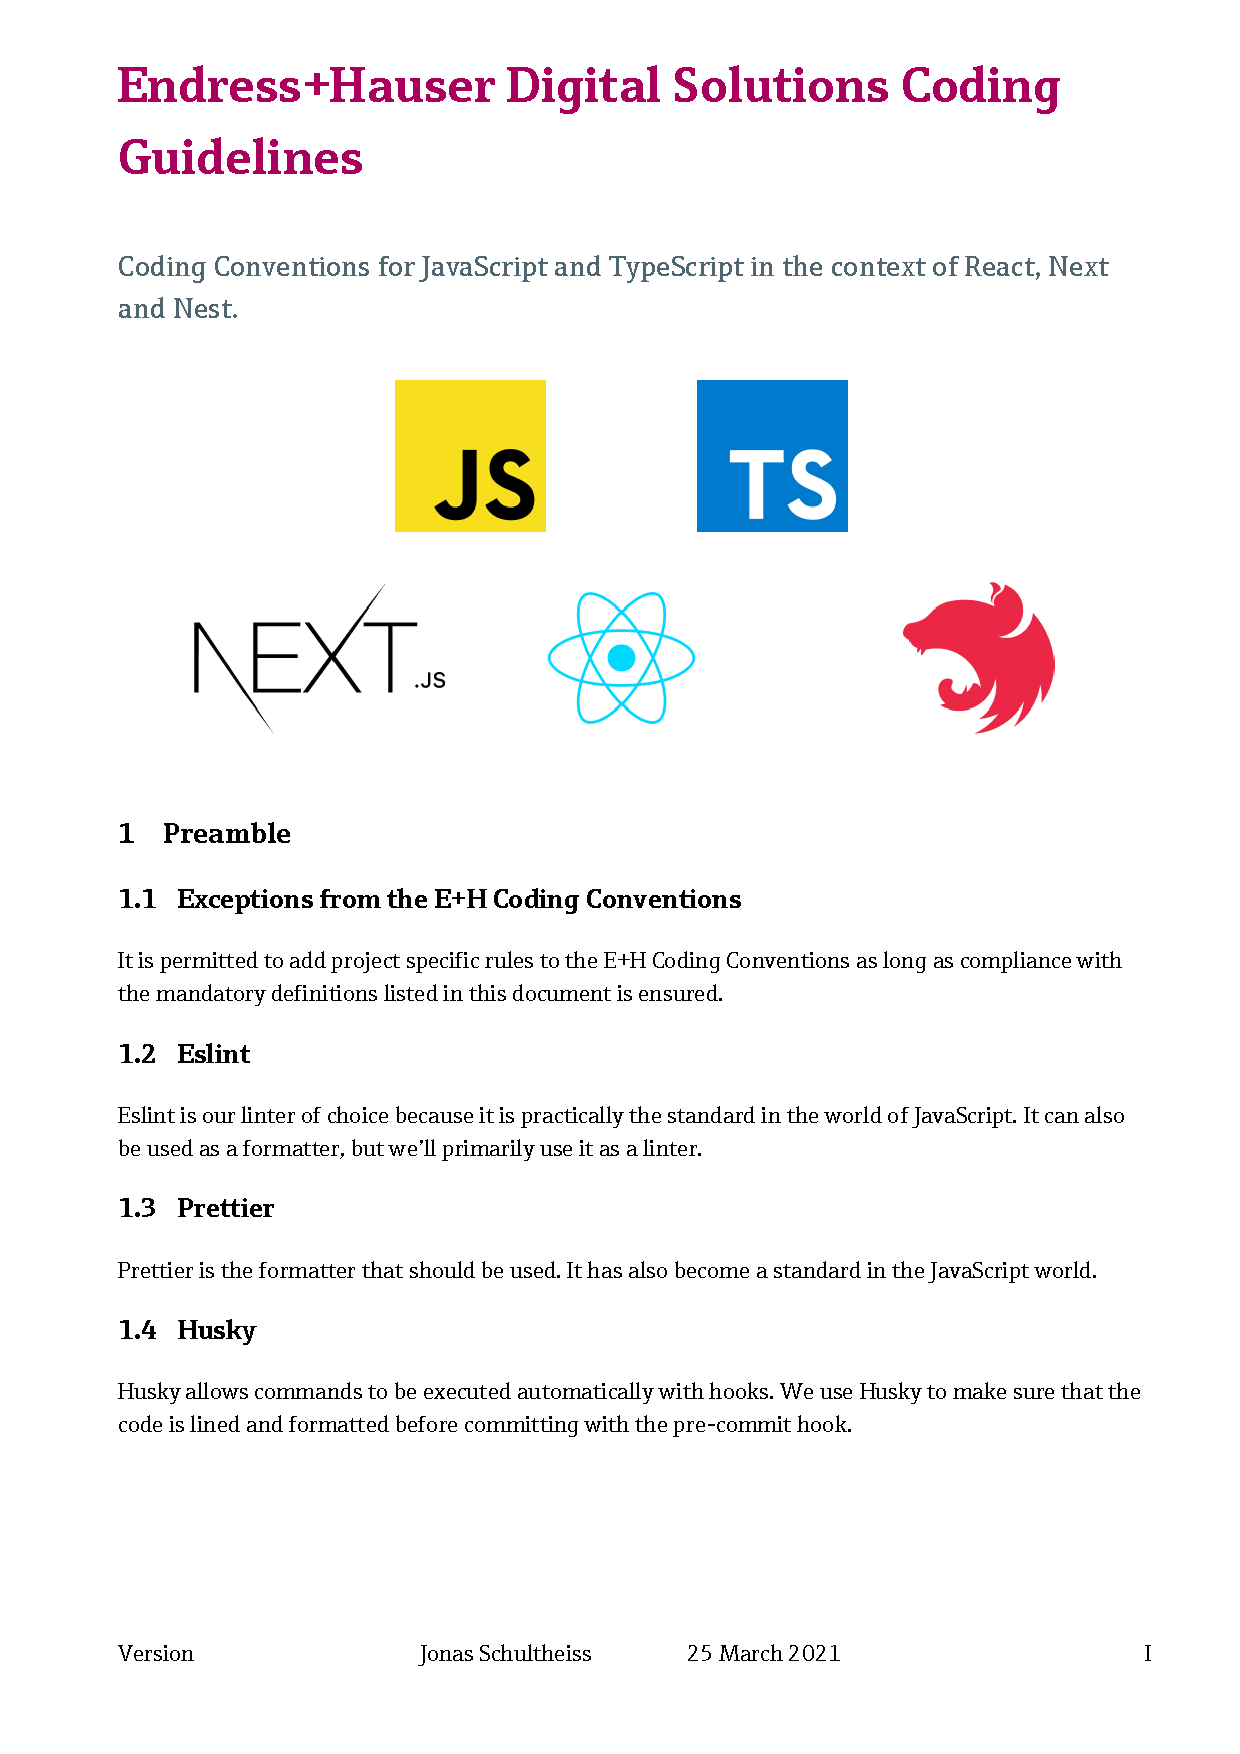
\includepdf[pages=-, scale=0.8]{./anhang/Endress+HauserDigitalSolutionsCodingGuidelinesJS.pdf}
  \end{appendix}
\end{document}